\documentclass[times]{article}

\usepackage[margin=1.0in]{geometry}
\usepackage{graphicx}
\usepackage{adjustbox}
\usepackage{float}
\usepackage{placeins}
\usepackage[none]{hyphenat}
\usepackage{amsmath}
\usepackage[us]{datetime}
\usepackage[explicit]{titlesec}
\usepackage{standalone}
\begin{document}
	\title{COMP SCI 5401 FS2017 Assignment 1b}
	\author{Dalton Cole \\ drcgy5@mst.edu}
	\date{\formatdate{9}{10}{2017}}
	\maketitle

	\section{Average vs Best Fitness}
	As can be seen from Figure %\ref{fig:graph_1001}


%	
%	\begin{figure}
%		\caption{F Test for Input 1 Assignment 1B vs 1A}
%		\label{fig:f_test1}
%		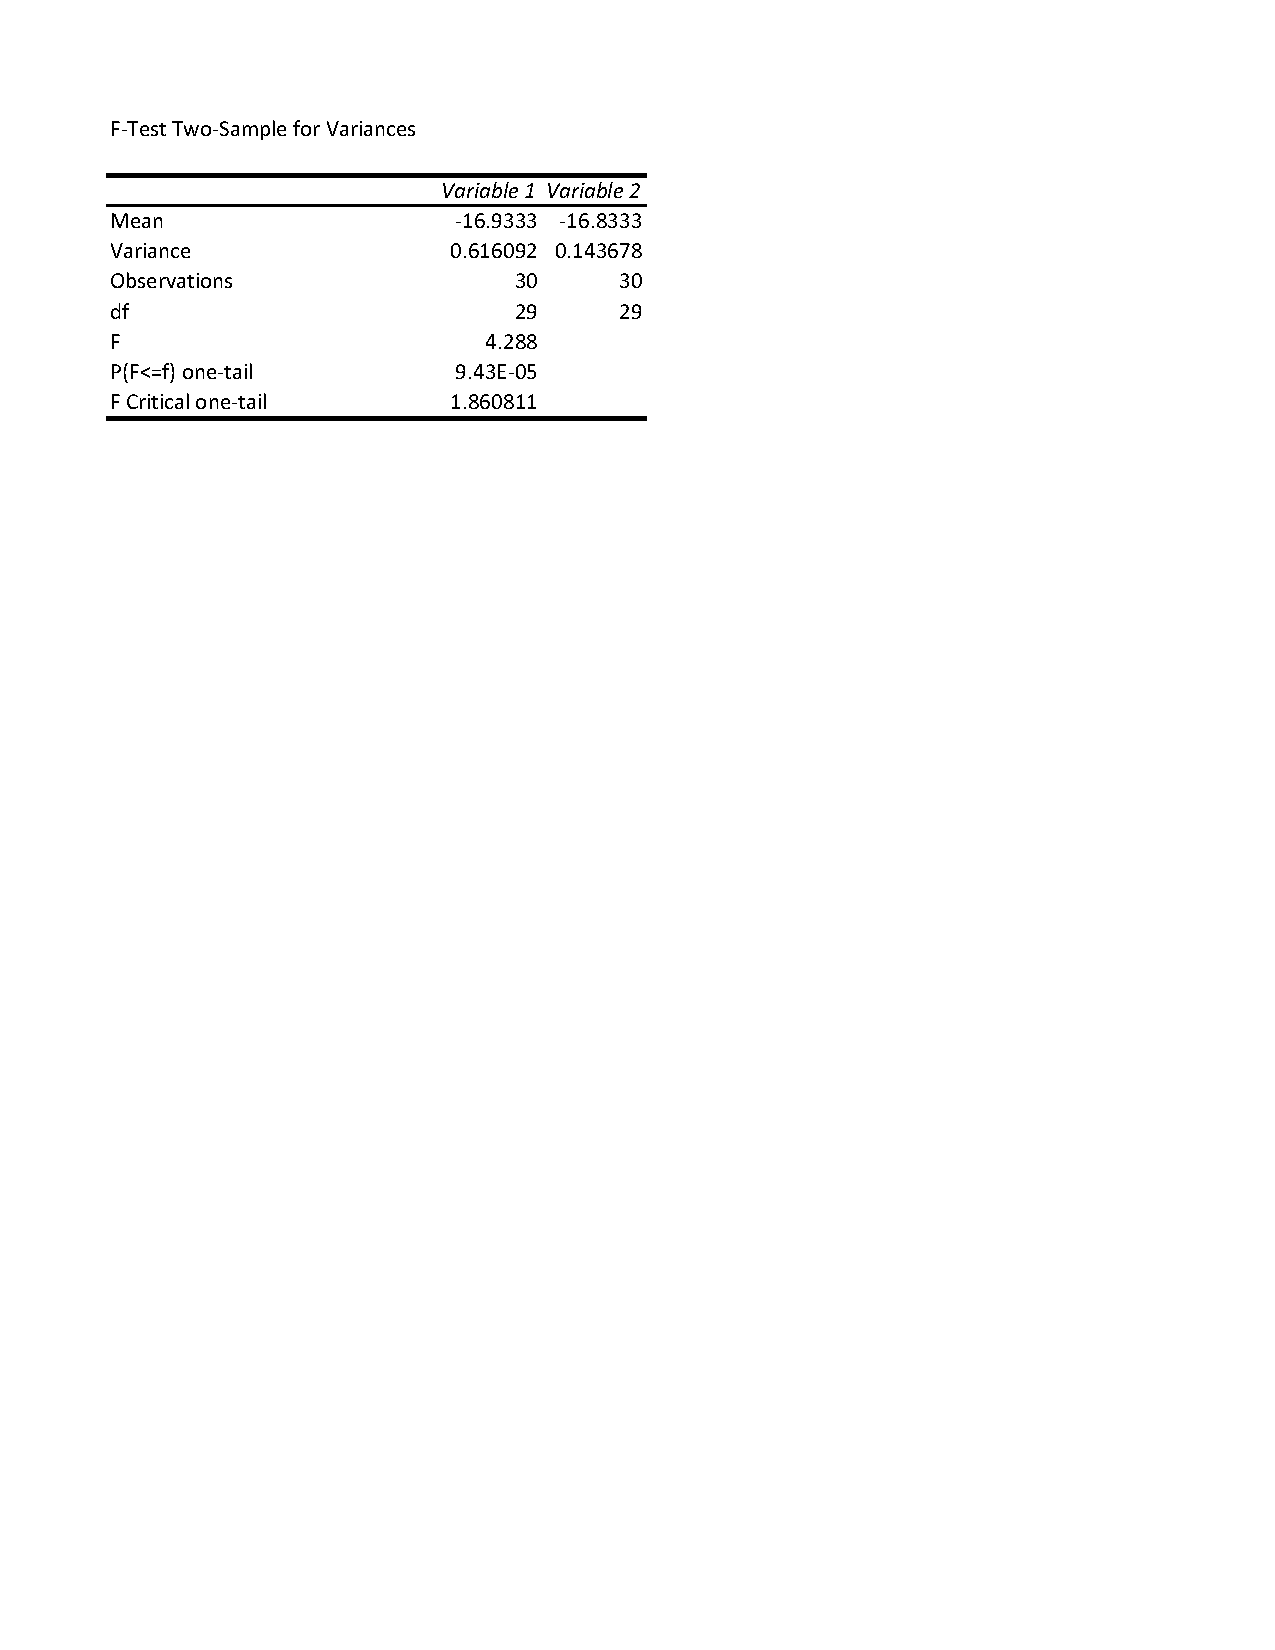
\includegraphics[width=\textwidth]{./tests/Input1_f_test.pdf}
%	\end{figure}


	\documentclass{standalone}
\begin{document}
\begin{table}[!htb]
	\centering
	\caption{Figure \ref{fig:graph_1001} Configuration File}
	\label{tab:graph_1001}
	\begin{tabular}{| c | c |}
		\hline
		Search Algorithm		& EA		 \\
		\hline
		Termination Convergence Criterion		& 10000		 \\
		\hline
		Fitness Evaluations		& 10000		 \\
		\hline
		Survival Strategy		& Plus		 \\
		\hline
		Mutation Algorithm		& Move		 \\
		\hline
		Placement Algorithm		& Random		 \\
		\hline
		Tournament Size For Parent Selection		& 5		 \\
		\hline
		Random Seed		& 1001		 \\
		\hline
		Self Adaptive Offspring Count		& False		 \\
		\hline
		Tournament Size For Survival Selection		& 5		 \\
		\hline
		Population Size		& 100		 \\
		\hline
		Survivor Algorithm		& Truncation		 \\
		\hline
		Offspring Count		& 50		 \\
		\hline
		Log File Path		& None		 \\
		\hline
		Penalty Coefficient		& 1		 \\
		\hline
		Parent Selection Algorithm		& k-Tournament Selection with replacement		 \\
		\hline
		Runs		& 30		 \\
		\hline
		Mutation Rate		& 0.1		 \\
		\hline
		Solution File Path		& None		 \\
		\hline
		Recombination Algorithm		& Partially Mapped Crossover		 \\
		\hline
		Self Adaptive Mutation Rate		& False		 \\
		\hline
		Self Adaptive Penalty Coefficient		& False		 \\
		\hline
	\end{tabular}
\end{table}
\begin{figure}[!htb]
	\caption{Input 1}
	\label{fig:graph_1001}
	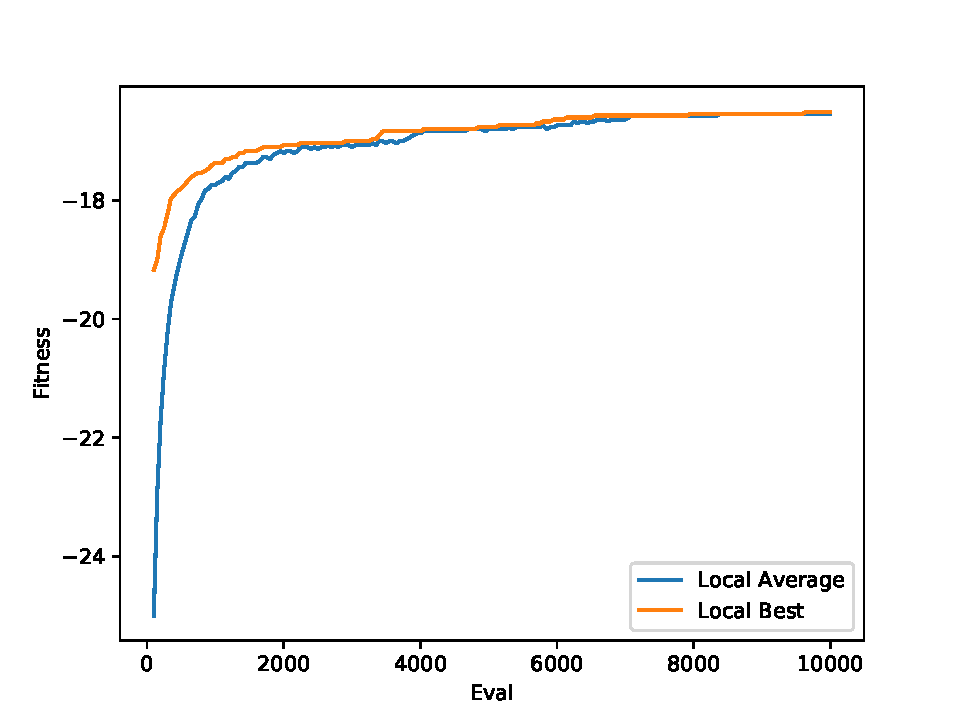
\includegraphics[width=\textwidth]{../graphs/graphs/1001.pdf}
\end{figure}


\begin{table}[!htb]
	\centering
	\caption{Figure \ref{fig:graph_1002} Configuration File}
	\label{tab:graph_1002}
	\begin{tabular}{| c | c |}
		\hline
		Search Algorithm		& EA		 \\
		\hline
		Termination Convergence Criterion		& 10000		 \\
		\hline
		Fitness Evaluations		& 10000		 \\
		\hline
		Survival Strategy		& Plus		 \\
		\hline
		Mutation Algorithm		& Move		 \\
		\hline
		Placement Algorithm		& Random		 \\
		\hline
		Tournament Size For Parent Selection		& 5		 \\
		\hline
		Random Seed		& 1002		 \\
		\hline
		Self Adaptive Offspring Count		& True		 \\
		\hline
		Tournament Size For Survival Selection		& 5		 \\
		\hline
		Population Size		& 100		 \\
		\hline
		Survivor Algorithm		& Truncation		 \\
		\hline
		Offspring Count		& 50		 \\
		\hline
		Log File Path		& None		 \\
		\hline
		Penalty Coefficient		& 1		 \\
		\hline
		Parent Selection Algorithm		& k-Tournament Selection with replacement		 \\
		\hline
		Runs		& 30		 \\
		\hline
		Mutation Rate		& 0.1		 \\
		\hline
		Solution File Path		& None		 \\
		\hline
		Recombination Algorithm		& Partially Mapped Crossover		 \\
		\hline
		Self Adaptive Mutation Rate		& False		 \\
		\hline
		Self Adaptive Penalty Coefficient		& False		 \\
		\hline
	\end{tabular}
\end{table}
\begin{figure}[!htb]
	\caption{Input 1}
	\label{fig:graph_1002}
	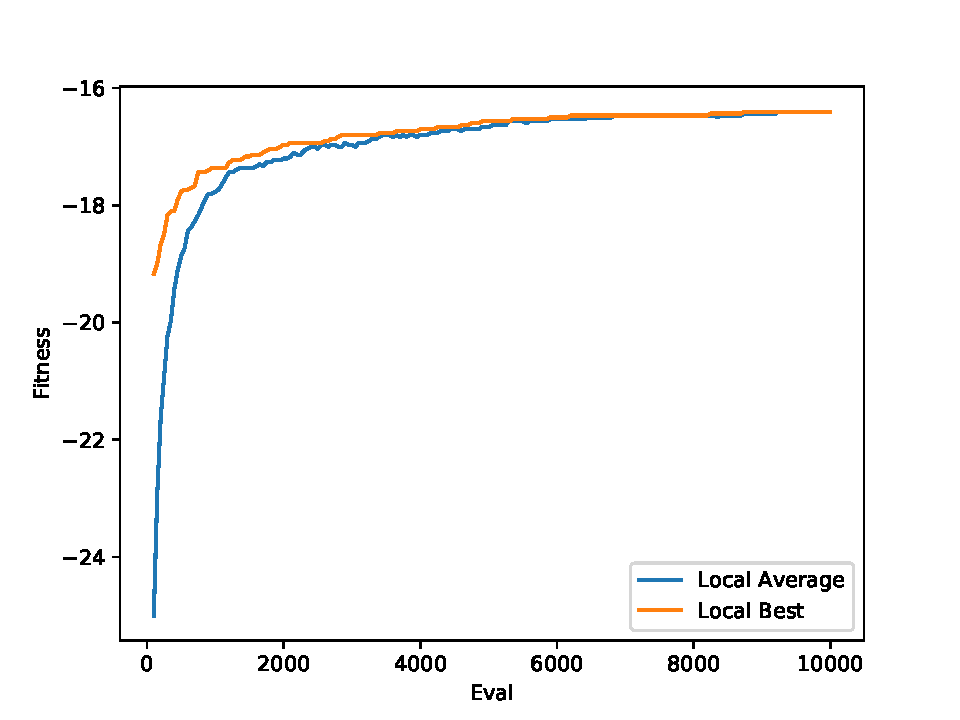
\includegraphics[width=\textwidth]{../graphs/graphs/1002.pdf}
\end{figure}


\begin{table}[!htb]
	\centering
	\caption{Figure \ref{fig:graph_1003} Configuration File}
	\label{tab:graph_1003}
	\begin{tabular}{| c | c |}
		\hline
		Search Algorithm		& EA		 \\
		\hline
		Termination Convergence Criterion		& 10000		 \\
		\hline
		Fitness Evaluations		& 10000		 \\
		\hline
		Survival Strategy		& Plus		 \\
		\hline
		Mutation Algorithm		& Move		 \\
		\hline
		Placement Algorithm		& Random		 \\
		\hline
		Tournament Size For Parent Selection		& 5		 \\
		\hline
		Random Seed		& 1003		 \\
		\hline
		Self Adaptive Offspring Count		& False		 \\
		\hline
		Tournament Size For Survival Selection		& 5		 \\
		\hline
		Population Size		& 100		 \\
		\hline
		Survivor Algorithm		& Truncation		 \\
		\hline
		Offspring Count		& 50		 \\
		\hline
		Log File Path		& None		 \\
		\hline
		Penalty Coefficient		& 1		 \\
		\hline
		Parent Selection Algorithm		& k-Tournament Selection with replacement		 \\
		\hline
		Runs		& 30		 \\
		\hline
		Mutation Rate		& 0.1		 \\
		\hline
		Solution File Path		& None		 \\
		\hline
		Recombination Algorithm		& Partially Mapped Crossover		 \\
		\hline
		Self Adaptive Mutation Rate		& False		 \\
		\hline
		Self Adaptive Penalty Coefficient		& True		 \\
		\hline
	\end{tabular}
\end{table}
\begin{figure}[!htb]
	\caption{Input 1}
	\label{fig:graph_1003}
	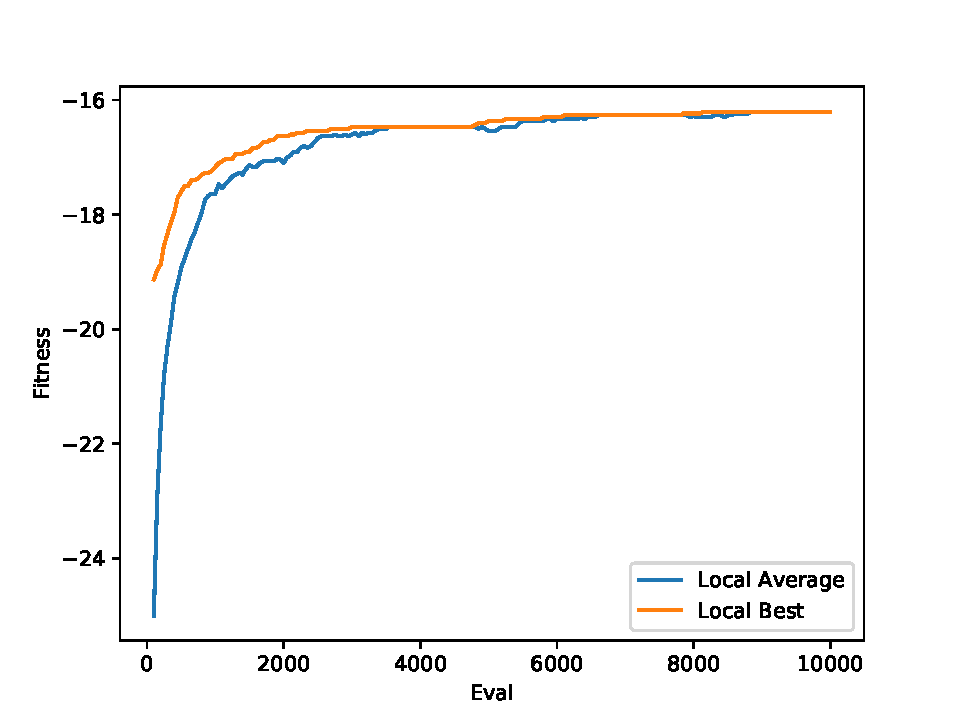
\includegraphics[width=\textwidth]{../graphs/graphs/1003.pdf}
\end{figure}


\begin{table}[!htb]
	\centering
	\caption{Figure \ref{fig:graph_1004} Configuration File}
	\label{tab:graph_1004}
	\begin{tabular}{| c | c |}
		\hline
		Search Algorithm		& EA		 \\
		\hline
		Termination Convergence Criterion		& 10000		 \\
		\hline
		Fitness Evaluations		& 10000		 \\
		\hline
		Survival Strategy		& Plus		 \\
		\hline
		Mutation Algorithm		& Move		 \\
		\hline
		Placement Algorithm		& Random		 \\
		\hline
		Tournament Size For Parent Selection		& 5		 \\
		\hline
		Random Seed		& 1004		 \\
		\hline
		Self Adaptive Offspring Count		& True		 \\
		\hline
		Tournament Size For Survival Selection		& 5		 \\
		\hline
		Population Size		& 100		 \\
		\hline
		Survivor Algorithm		& Truncation		 \\
		\hline
		Offspring Count		& 50		 \\
		\hline
		Log File Path		& None		 \\
		\hline
		Penalty Coefficient		& 1		 \\
		\hline
		Parent Selection Algorithm		& k-Tournament Selection with replacement		 \\
		\hline
		Runs		& 30		 \\
		\hline
		Mutation Rate		& 0.1		 \\
		\hline
		Solution File Path		& None		 \\
		\hline
		Recombination Algorithm		& Partially Mapped Crossover		 \\
		\hline
		Self Adaptive Mutation Rate		& False		 \\
		\hline
		Self Adaptive Penalty Coefficient		& True		 \\
		\hline
	\end{tabular}
\end{table}
\begin{figure}[!htb]
	\caption{Input 1}
	\label{fig:graph_1004}
	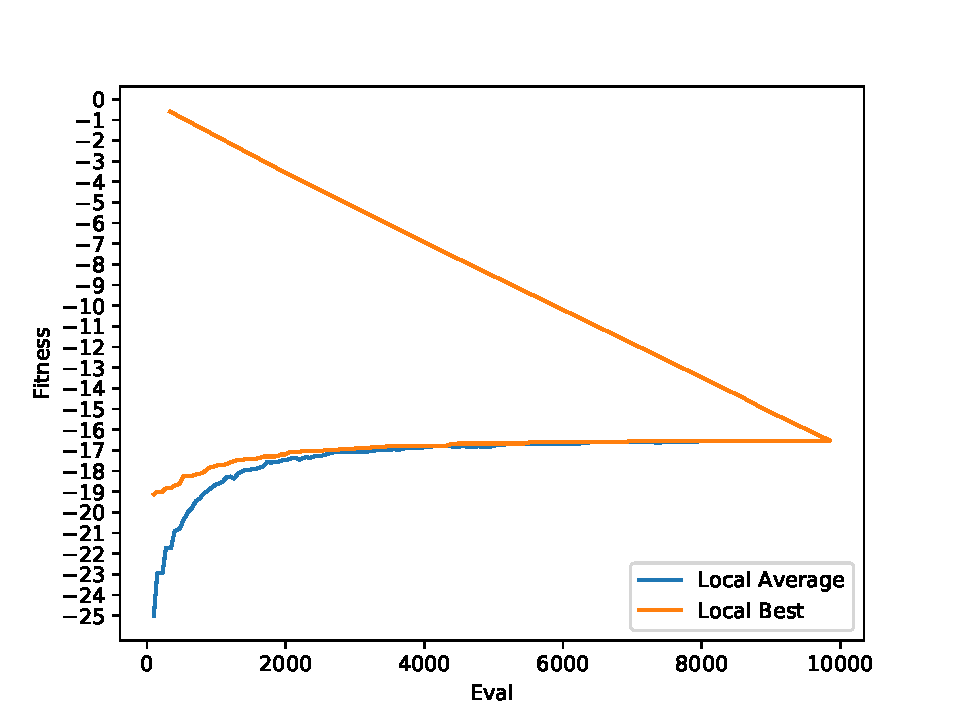
\includegraphics[width=\textwidth]{../graphs/graphs/1004.pdf}
\end{figure}


\begin{table}[!htb]
	\centering
	\caption{Figure \ref{fig:graph_1005} Configuration File}
	\label{tab:graph_1005}
	\begin{tabular}{| c | c |}
		\hline
		Search Algorithm		& EA		 \\
		\hline
		Termination Convergence Criterion		& 10000		 \\
		\hline
		Fitness Evaluations		& 10000		 \\
		\hline
		Survival Strategy		& Plus		 \\
		\hline
		Mutation Algorithm		& Move		 \\
		\hline
		Placement Algorithm		& Random		 \\
		\hline
		Tournament Size For Parent Selection		& 5		 \\
		\hline
		Random Seed		& 1005		 \\
		\hline
		Self Adaptive Offspring Count		& False		 \\
		\hline
		Tournament Size For Survival Selection		& 5		 \\
		\hline
		Population Size		& 100		 \\
		\hline
		Survivor Algorithm		& Truncation		 \\
		\hline
		Offspring Count		& 50		 \\
		\hline
		Log File Path		& None		 \\
		\hline
		Penalty Coefficient		& 1		 \\
		\hline
		Parent Selection Algorithm		& k-Tournament Selection with replacement		 \\
		\hline
		Runs		& 30		 \\
		\hline
		Mutation Rate		& 0.1		 \\
		\hline
		Solution File Path		& None		 \\
		\hline
		Recombination Algorithm		& Partially Mapped Crossover		 \\
		\hline
		Self Adaptive Mutation Rate		& True		 \\
		\hline
		Self Adaptive Penalty Coefficient		& False		 \\
		\hline
	\end{tabular}
\end{table}
\begin{figure}[!htb]
	\caption{Input 1}
	\label{fig:graph_1005}
	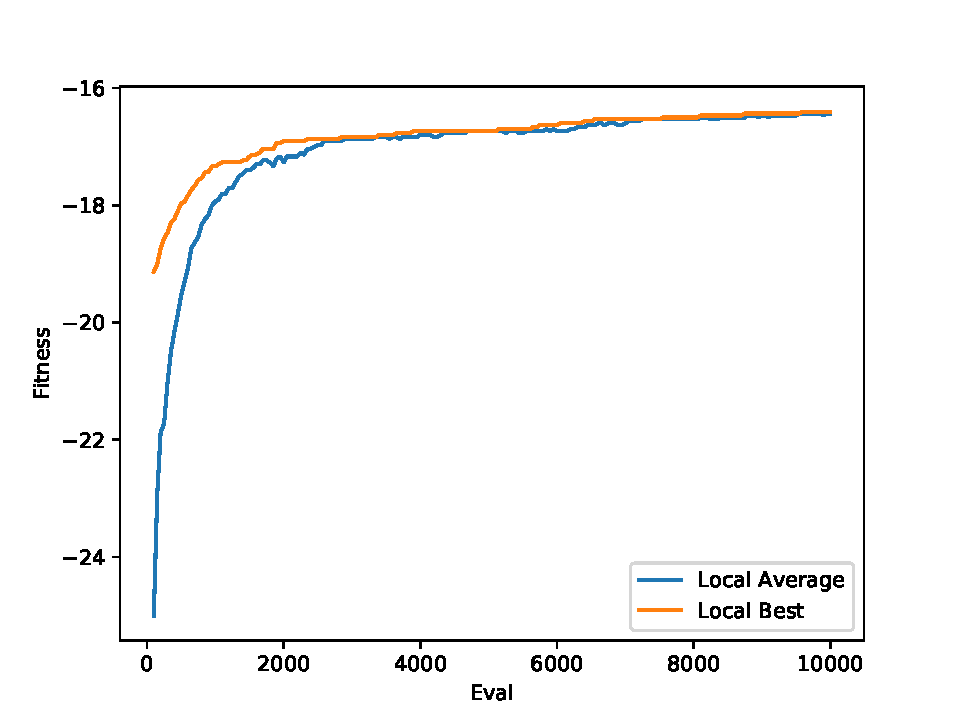
\includegraphics[width=\textwidth]{../graphs/graphs/1005.pdf}
\end{figure}


\begin{table}[!htb]
	\centering
	\caption{Figure \ref{fig:graph_1006} Configuration File}
	\label{tab:graph_1006}
	\begin{tabular}{| c | c |}
		\hline
		Search Algorithm		& EA		 \\
		\hline
		Termination Convergence Criterion		& 10000		 \\
		\hline
		Fitness Evaluations		& 10000		 \\
		\hline
		Survival Strategy		& Plus		 \\
		\hline
		Mutation Algorithm		& Move		 \\
		\hline
		Placement Algorithm		& Random		 \\
		\hline
		Tournament Size For Parent Selection		& 5		 \\
		\hline
		Random Seed		& 1006		 \\
		\hline
		Self Adaptive Offspring Count		& True		 \\
		\hline
		Tournament Size For Survival Selection		& 5		 \\
		\hline
		Population Size		& 100		 \\
		\hline
		Survivor Algorithm		& Truncation		 \\
		\hline
		Offspring Count		& 50		 \\
		\hline
		Log File Path		& None		 \\
		\hline
		Penalty Coefficient		& 1		 \\
		\hline
		Parent Selection Algorithm		& k-Tournament Selection with replacement		 \\
		\hline
		Runs		& 30		 \\
		\hline
		Mutation Rate		& 0.1		 \\
		\hline
		Solution File Path		& None		 \\
		\hline
		Recombination Algorithm		& Partially Mapped Crossover		 \\
		\hline
		Self Adaptive Mutation Rate		& True		 \\
		\hline
		Self Adaptive Penalty Coefficient		& False		 \\
		\hline
	\end{tabular}
\end{table}
\begin{figure}[!htb]
	\caption{Input 1}
	\label{fig:graph_1006}
	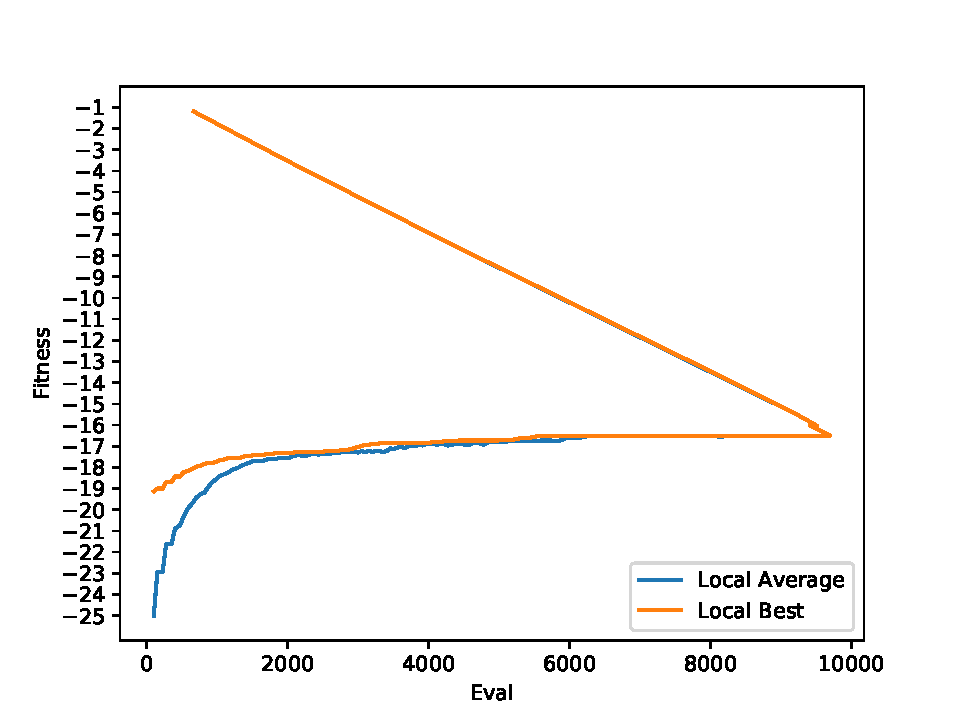
\includegraphics[width=\textwidth]{../graphs/graphs/1006.pdf}
\end{figure}


\begin{table}[!htb]
	\centering
	\caption{Figure \ref{fig:graph_1007} Configuration File}
	\label{tab:graph_1007}
	\begin{tabular}{| c | c |}
		\hline
		Search Algorithm		& EA		 \\
		\hline
		Termination Convergence Criterion		& 10000		 \\
		\hline
		Fitness Evaluations		& 10000		 \\
		\hline
		Survival Strategy		& Plus		 \\
		\hline
		Mutation Algorithm		& Move		 \\
		\hline
		Placement Algorithm		& Random		 \\
		\hline
		Tournament Size For Parent Selection		& 5		 \\
		\hline
		Random Seed		& 1007		 \\
		\hline
		Self Adaptive Offspring Count		& False		 \\
		\hline
		Tournament Size For Survival Selection		& 5		 \\
		\hline
		Population Size		& 100		 \\
		\hline
		Survivor Algorithm		& Truncation		 \\
		\hline
		Offspring Count		& 50		 \\
		\hline
		Log File Path		& None		 \\
		\hline
		Penalty Coefficient		& 1		 \\
		\hline
		Parent Selection Algorithm		& k-Tournament Selection with replacement		 \\
		\hline
		Runs		& 30		 \\
		\hline
		Mutation Rate		& 0.1		 \\
		\hline
		Solution File Path		& None		 \\
		\hline
		Recombination Algorithm		& Partially Mapped Crossover		 \\
		\hline
		Self Adaptive Mutation Rate		& True		 \\
		\hline
		Self Adaptive Penalty Coefficient		& True		 \\
		\hline
	\end{tabular}
\end{table}
\begin{figure}[!htb]
	\caption{Input 1}
	\label{fig:graph_1007}
	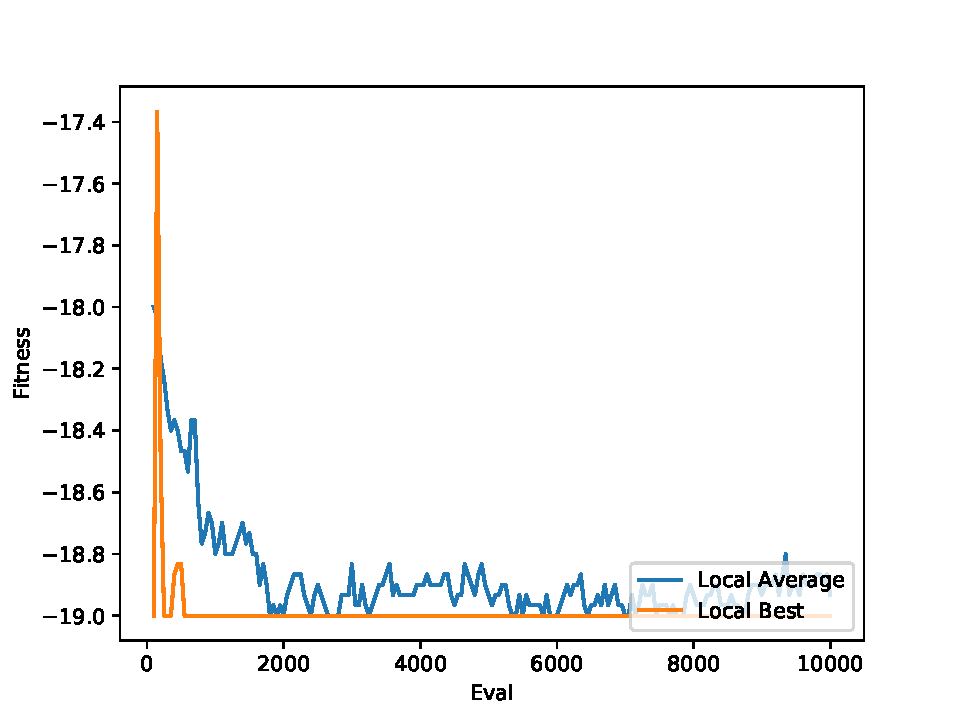
\includegraphics[width=\textwidth]{../graphs/graphs/1007.pdf}
\end{figure}


\begin{table}[!htb]
	\centering
	\caption{Figure \ref{fig:graph_1008} Configuration File}
	\label{tab:graph_1008}
	\begin{tabular}{| c | c |}
		\hline
		Search Algorithm		& EA		 \\
		\hline
		Termination Convergence Criterion		& 10000		 \\
		\hline
		Fitness Evaluations		& 10000		 \\
		\hline
		Survival Strategy		& Plus		 \\
		\hline
		Mutation Algorithm		& Move		 \\
		\hline
		Placement Algorithm		& Random		 \\
		\hline
		Tournament Size For Parent Selection		& 5		 \\
		\hline
		Random Seed		& 1008		 \\
		\hline
		Self Adaptive Offspring Count		& True		 \\
		\hline
		Tournament Size For Survival Selection		& 5		 \\
		\hline
		Population Size		& 100		 \\
		\hline
		Survivor Algorithm		& Truncation		 \\
		\hline
		Offspring Count		& 50		 \\
		\hline
		Log File Path		& None		 \\
		\hline
		Penalty Coefficient		& 1		 \\
		\hline
		Parent Selection Algorithm		& k-Tournament Selection with replacement		 \\
		\hline
		Runs		& 30		 \\
		\hline
		Mutation Rate		& 0.1		 \\
		\hline
		Solution File Path		& None		 \\
		\hline
		Recombination Algorithm		& Partially Mapped Crossover		 \\
		\hline
		Self Adaptive Mutation Rate		& True		 \\
		\hline
		Self Adaptive Penalty Coefficient		& True		 \\
		\hline
	\end{tabular}
\end{table}
\begin{figure}[!htb]
	\caption{Input 1}
	\label{fig:graph_1008}
	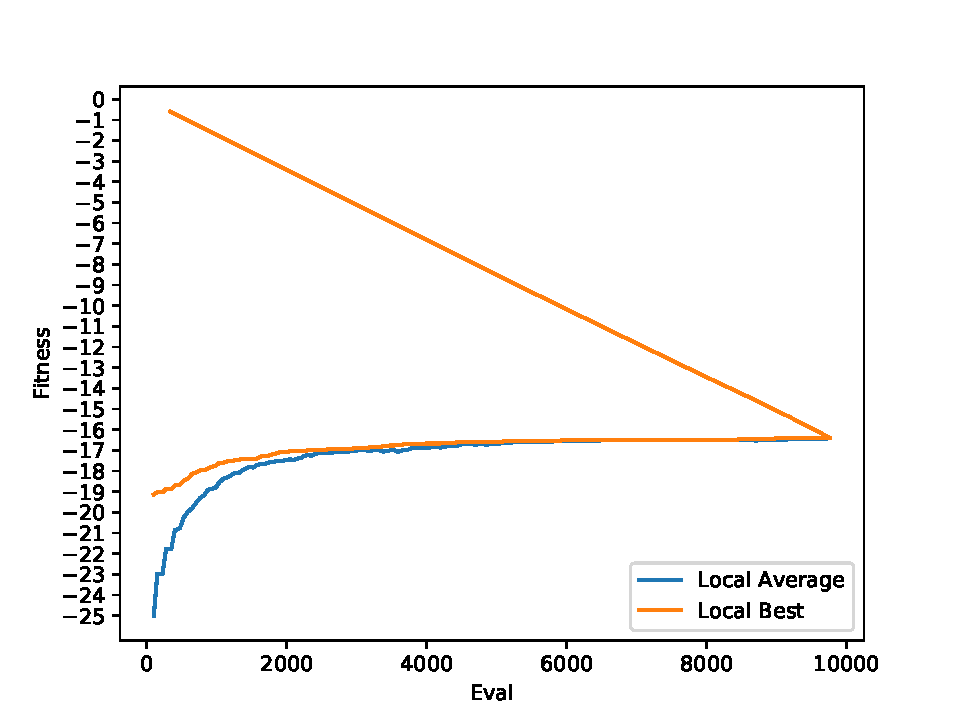
\includegraphics[width=\textwidth]{../graphs/graphs/1008.pdf}
\end{figure}


\begin{table}[!htb]
	\centering
	\caption{Figure \ref{fig:graph_1009} Configuration File}
	\label{tab:graph_1009}
	\begin{tabular}{| c | c |}
		\hline
		Search Algorithm		& EA		 \\
		\hline
		Termination Convergence Criterion		& 10000		 \\
		\hline
		Fitness Evaluations		& 10000		 \\
		\hline
		Survival Strategy		& Plus		 \\
		\hline
		Mutation Algorithm		& Move		 \\
		\hline
		Placement Algorithm		& Random with Repair		 \\
		\hline
		Tournament Size For Parent Selection		& 5		 \\
		\hline
		Random Seed		& 1009		 \\
		\hline
		Self Adaptive Offspring Count		& False		 \\
		\hline
		Tournament Size For Survival Selection		& 5		 \\
		\hline
		Population Size		& 100		 \\
		\hline
		Survivor Algorithm		& Truncation		 \\
		\hline
		Offspring Count		& 50		 \\
		\hline
		Log File Path		& None		 \\
		\hline
		Penalty Coefficient		& 1		 \\
		\hline
		Parent Selection Algorithm		& k-Tournament Selection with replacement		 \\
		\hline
		Runs		& 30		 \\
		\hline
		Mutation Rate		& 0.1		 \\
		\hline
		Solution File Path		& None		 \\
		\hline
		Recombination Algorithm		& Partially Mapped Crossover		 \\
		\hline
		Self Adaptive Mutation Rate		& False		 \\
		\hline
		Self Adaptive Penalty Coefficient		& False		 \\
		\hline
	\end{tabular}
\end{table}
\begin{figure}[!htb]
	\caption{Input 1}
	\label{fig:graph_1009}
	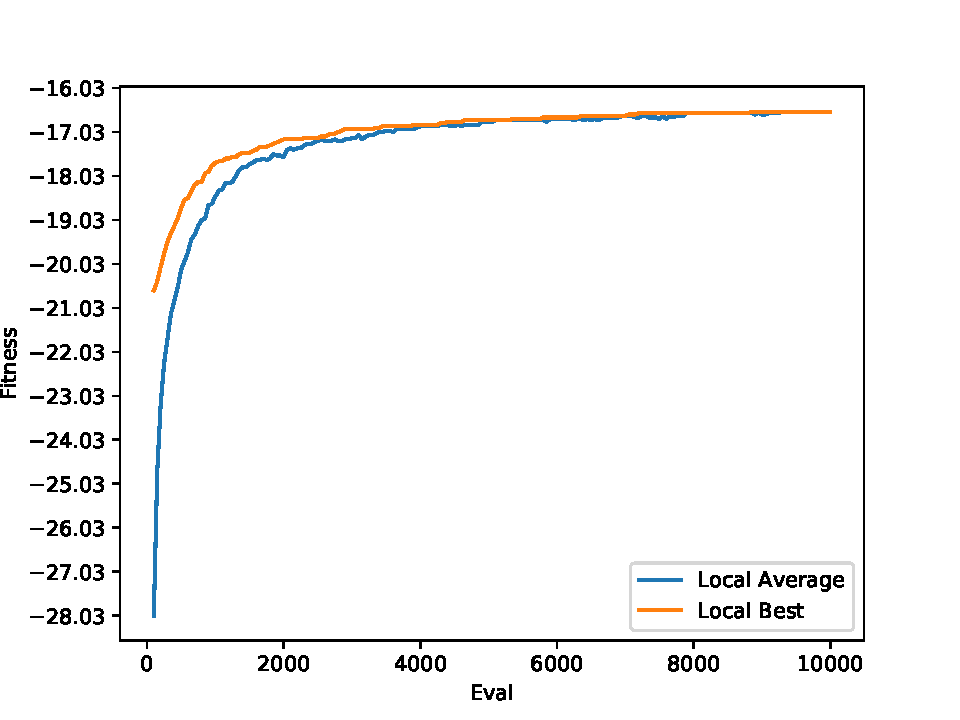
\includegraphics[width=\textwidth]{../graphs/graphs/1009.pdf}
\end{figure}


\begin{table}[!htb]
	\centering
	\caption{Figure \ref{fig:graph_1010} Configuration File}
	\label{tab:graph_1010}
	\begin{tabular}{| c | c |}
		\hline
		Search Algorithm		& EA		 \\
		\hline
		Termination Convergence Criterion		& 10000		 \\
		\hline
		Fitness Evaluations		& 10000		 \\
		\hline
		Survival Strategy		& Plus		 \\
		\hline
		Mutation Algorithm		& Move		 \\
		\hline
		Placement Algorithm		& Random with Repair		 \\
		\hline
		Tournament Size For Parent Selection		& 5		 \\
		\hline
		Random Seed		& 1010		 \\
		\hline
		Self Adaptive Offspring Count		& True		 \\
		\hline
		Tournament Size For Survival Selection		& 5		 \\
		\hline
		Population Size		& 100		 \\
		\hline
		Survivor Algorithm		& Truncation		 \\
		\hline
		Offspring Count		& 50		 \\
		\hline
		Log File Path		& None		 \\
		\hline
		Penalty Coefficient		& 1		 \\
		\hline
		Parent Selection Algorithm		& k-Tournament Selection with replacement		 \\
		\hline
		Runs		& 30		 \\
		\hline
		Mutation Rate		& 0.1		 \\
		\hline
		Solution File Path		& None		 \\
		\hline
		Recombination Algorithm		& Partially Mapped Crossover		 \\
		\hline
		Self Adaptive Mutation Rate		& False		 \\
		\hline
		Self Adaptive Penalty Coefficient		& False		 \\
		\hline
	\end{tabular}
\end{table}
\begin{figure}[!htb]
	\caption{Input 1}
	\label{fig:graph_1010}
	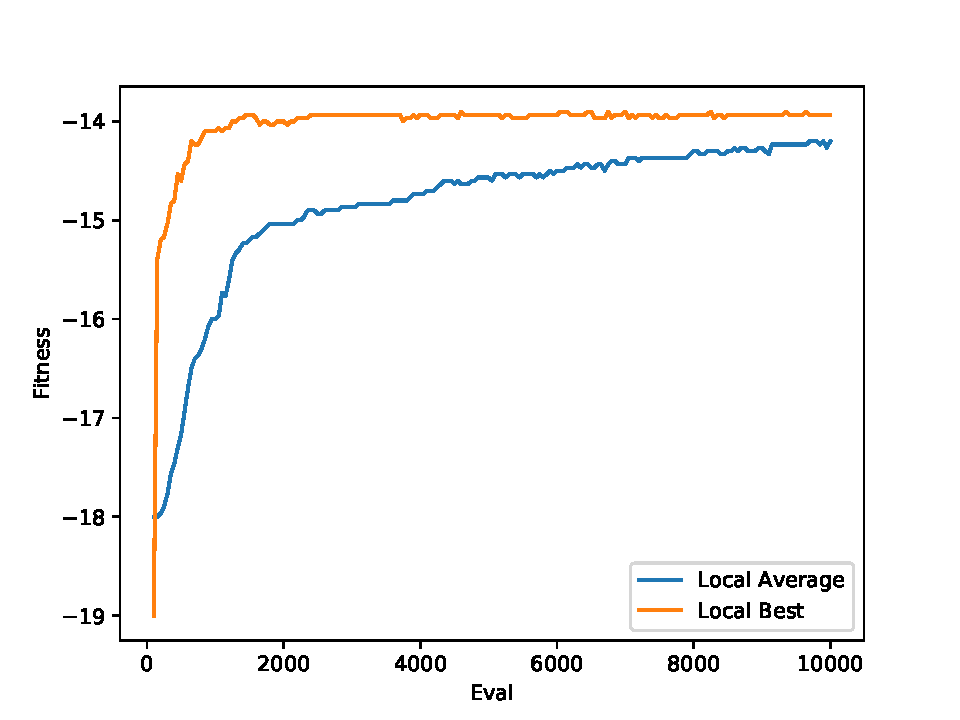
\includegraphics[width=\textwidth]{../graphs/graphs/1010.pdf}
\end{figure}


\clearpage
\begin{table}[!htb]
	\centering
	\caption{Figure \ref{fig:graph_1011} Configuration File}
	\label{tab:graph_1011}
	\begin{tabular}{| c | c |}
		\hline
		Search Algorithm		& EA		 \\
		\hline
		Termination Convergence Criterion		& 10000		 \\
		\hline
		Fitness Evaluations		& 10000		 \\
		\hline
		Survival Strategy		& Plus		 \\
		\hline
		Mutation Algorithm		& Move		 \\
		\hline
		Placement Algorithm		& Random with Repair		 \\
		\hline
		Tournament Size For Parent Selection		& 5		 \\
		\hline
		Random Seed		& 1011		 \\
		\hline
		Self Adaptive Offspring Count		& False		 \\
		\hline
		Tournament Size For Survival Selection		& 5		 \\
		\hline
		Population Size		& 100		 \\
		\hline
		Survivor Algorithm		& Truncation		 \\
		\hline
		Offspring Count		& 50		 \\
		\hline
		Log File Path		& None		 \\
		\hline
		Penalty Coefficient		& 1		 \\
		\hline
		Parent Selection Algorithm		& k-Tournament Selection with replacement		 \\
		\hline
		Runs		& 30		 \\
		\hline
		Mutation Rate		& 0.1		 \\
		\hline
		Solution File Path		& None		 \\
		\hline
		Recombination Algorithm		& Partially Mapped Crossover		 \\
		\hline
		Self Adaptive Mutation Rate		& False		 \\
		\hline
		Self Adaptive Penalty Coefficient		& True		 \\
		\hline
	\end{tabular}
\end{table}
\begin{figure}[!htb]
	\caption{Input 1}
	\label{fig:graph_1011}
	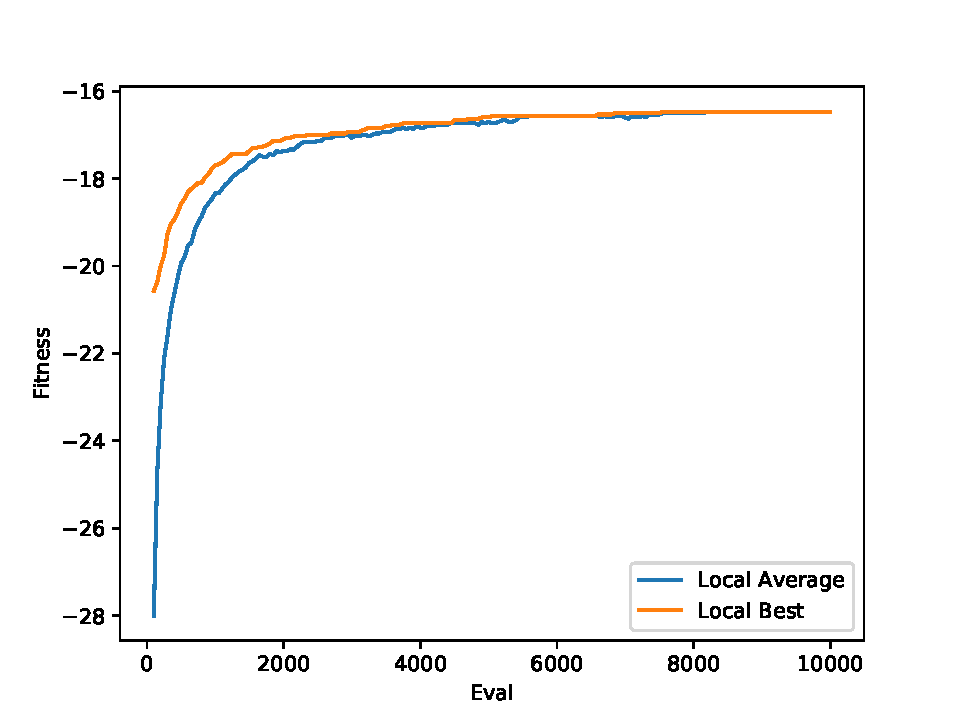
\includegraphics[width=\textwidth]{../graphs/graphs/1011.pdf}
\end{figure}


\begin{table}[!htb]
	\centering
	\caption{Figure \ref{fig:graph_1012} Configuration File}
	\label{tab:graph_1012}
	\begin{tabular}{| c | c |}
		\hline
		Search Algorithm		& EA		 \\
		\hline
		Termination Convergence Criterion		& 10000		 \\
		\hline
		Fitness Evaluations		& 10000		 \\
		\hline
		Survival Strategy		& Plus		 \\
		\hline
		Mutation Algorithm		& Move		 \\
		\hline
		Placement Algorithm		& Random with Repair		 \\
		\hline
		Tournament Size For Parent Selection		& 5		 \\
		\hline
		Random Seed		& 1012		 \\
		\hline
		Self Adaptive Offspring Count		& True		 \\
		\hline
		Tournament Size For Survival Selection		& 5		 \\
		\hline
		Population Size		& 100		 \\
		\hline
		Survivor Algorithm		& Truncation		 \\
		\hline
		Offspring Count		& 50		 \\
		\hline
		Log File Path		& None		 \\
		\hline
		Penalty Coefficient		& 1		 \\
		\hline
		Parent Selection Algorithm		& k-Tournament Selection with replacement		 \\
		\hline
		Runs		& 30		 \\
		\hline
		Mutation Rate		& 0.1		 \\
		\hline
		Solution File Path		& None		 \\
		\hline
		Recombination Algorithm		& Partially Mapped Crossover		 \\
		\hline
		Self Adaptive Mutation Rate		& False		 \\
		\hline
		Self Adaptive Penalty Coefficient		& True		 \\
		\hline
	\end{tabular}
\end{table}
\begin{figure}[!htb]
	\caption{Input 1}
	\label{fig:graph_1012}
	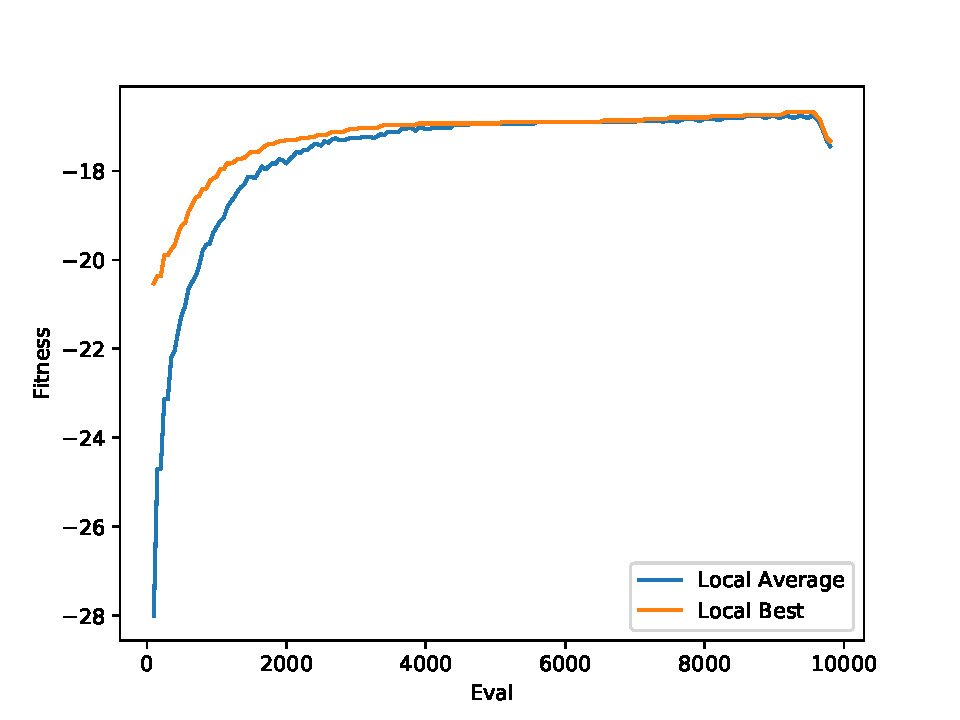
\includegraphics[width=\textwidth]{../graphs/graphs/1012.pdf}
\end{figure}


\begin{table}[!htb]
	\centering
	\caption{Figure \ref{fig:graph_1013} Configuration File}
	\label{tab:graph_1013}
	\begin{tabular}{| c | c |}
		\hline
		Search Algorithm		& EA		 \\
		\hline
		Termination Convergence Criterion		& 10000		 \\
		\hline
		Fitness Evaluations		& 10000		 \\
		\hline
		Survival Strategy		& Plus		 \\
		\hline
		Mutation Algorithm		& Move		 \\
		\hline
		Placement Algorithm		& Random with Repair		 \\
		\hline
		Tournament Size For Parent Selection		& 5		 \\
		\hline
		Random Seed		& 1013		 \\
		\hline
		Self Adaptive Offspring Count		& False		 \\
		\hline
		Tournament Size For Survival Selection		& 5		 \\
		\hline
		Population Size		& 100		 \\
		\hline
		Survivor Algorithm		& Truncation		 \\
		\hline
		Offspring Count		& 50		 \\
		\hline
		Log File Path		& None		 \\
		\hline
		Penalty Coefficient		& 1		 \\
		\hline
		Parent Selection Algorithm		& k-Tournament Selection with replacement		 \\
		\hline
		Runs		& 30		 \\
		\hline
		Mutation Rate		& 0.1		 \\
		\hline
		Solution File Path		& None		 \\
		\hline
		Recombination Algorithm		& Partially Mapped Crossover		 \\
		\hline
		Self Adaptive Mutation Rate		& True		 \\
		\hline
		Self Adaptive Penalty Coefficient		& False		 \\
		\hline
	\end{tabular}
\end{table}
\begin{figure}[!htb]
	\caption{Input 1}
	\label{fig:graph_1013}
	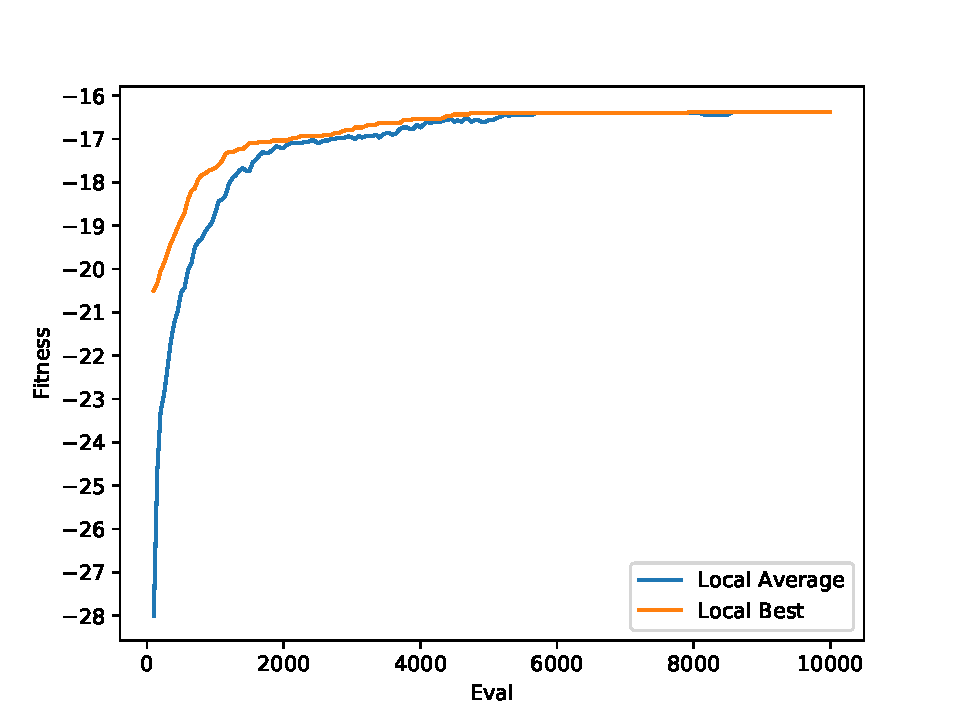
\includegraphics[width=\textwidth]{../graphs/graphs/1013.pdf}
\end{figure}


\begin{table}[!htb]
	\centering
	\caption{Figure \ref{fig:graph_1014} Configuration File}
	\label{tab:graph_1014}
	\begin{tabular}{| c | c |}
		\hline
		Search Algorithm		& EA		 \\
		\hline
		Termination Convergence Criterion		& 10000		 \\
		\hline
		Fitness Evaluations		& 10000		 \\
		\hline
		Survival Strategy		& Plus		 \\
		\hline
		Mutation Algorithm		& Move		 \\
		\hline
		Placement Algorithm		& Random with Repair		 \\
		\hline
		Tournament Size For Parent Selection		& 5		 \\
		\hline
		Random Seed		& 1014		 \\
		\hline
		Self Adaptive Offspring Count		& True		 \\
		\hline
		Tournament Size For Survival Selection		& 5		 \\
		\hline
		Population Size		& 100		 \\
		\hline
		Survivor Algorithm		& Truncation		 \\
		\hline
		Offspring Count		& 50		 \\
		\hline
		Log File Path		& None		 \\
		\hline
		Penalty Coefficient		& 1		 \\
		\hline
		Parent Selection Algorithm		& k-Tournament Selection with replacement		 \\
		\hline
		Runs		& 30		 \\
		\hline
		Mutation Rate		& 0.1		 \\
		\hline
		Solution File Path		& None		 \\
		\hline
		Recombination Algorithm		& Partially Mapped Crossover		 \\
		\hline
		Self Adaptive Mutation Rate		& True		 \\
		\hline
		Self Adaptive Penalty Coefficient		& False		 \\
		\hline
	\end{tabular}
\end{table}
\begin{figure}[!htb]
	\caption{Input 1}
	\label{fig:graph_1014}
	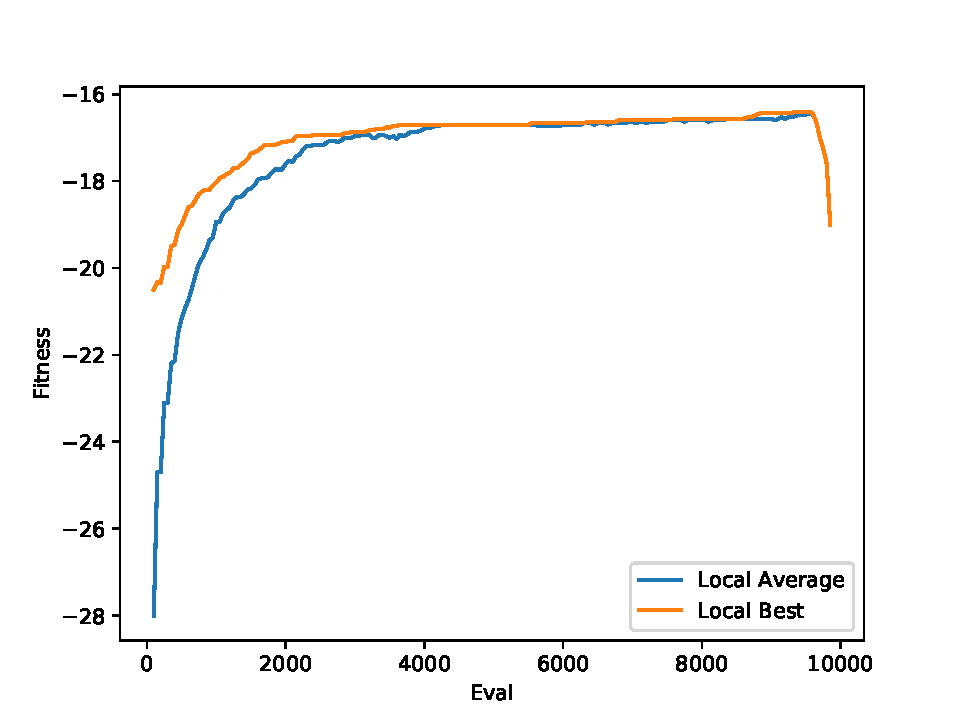
\includegraphics[width=\textwidth]{../graphs/graphs/1014.pdf}
\end{figure}


\begin{table}[!htb]
	\centering
	\caption{Figure \ref{fig:graph_1015} Configuration File}
	\label{tab:graph_1015}
	\begin{tabular}{| c | c |}
		\hline
		Search Algorithm		& EA		 \\
		\hline
		Termination Convergence Criterion		& 10000		 \\
		\hline
		Fitness Evaluations		& 10000		 \\
		\hline
		Survival Strategy		& Plus		 \\
		\hline
		Mutation Algorithm		& Move		 \\
		\hline
		Placement Algorithm		& Random with Repair		 \\
		\hline
		Tournament Size For Parent Selection		& 5		 \\
		\hline
		Random Seed		& 1015		 \\
		\hline
		Self Adaptive Offspring Count		& False		 \\
		\hline
		Tournament Size For Survival Selection		& 5		 \\
		\hline
		Population Size		& 100		 \\
		\hline
		Survivor Algorithm		& Truncation		 \\
		\hline
		Offspring Count		& 50		 \\
		\hline
		Log File Path		& None		 \\
		\hline
		Penalty Coefficient		& 1		 \\
		\hline
		Parent Selection Algorithm		& k-Tournament Selection with replacement		 \\
		\hline
		Runs		& 30		 \\
		\hline
		Mutation Rate		& 0.1		 \\
		\hline
		Solution File Path		& None		 \\
		\hline
		Recombination Algorithm		& Partially Mapped Crossover		 \\
		\hline
		Self Adaptive Mutation Rate		& True		 \\
		\hline
		Self Adaptive Penalty Coefficient		& True		 \\
		\hline
	\end{tabular}
\end{table}
\begin{figure}[!htb]
	\caption{Input 1}
	\label{fig:graph_1015}
	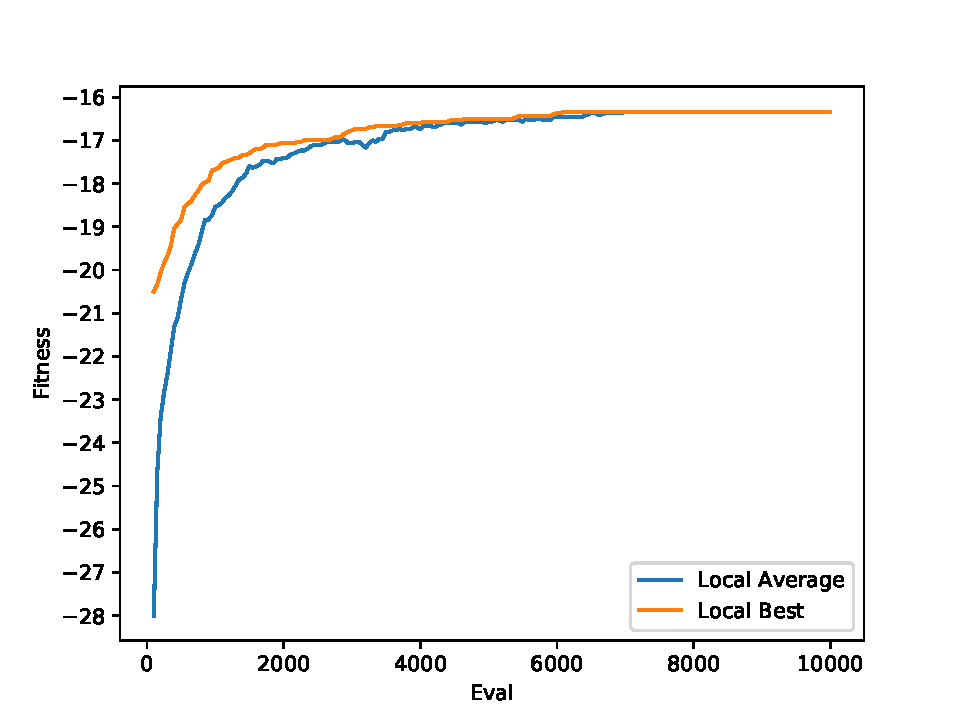
\includegraphics[width=\textwidth]{../graphs/graphs/1015.pdf}
\end{figure}


\begin{table}[!htb]
	\centering
	\caption{Figure \ref{fig:graph_1016} Configuration File}
	\label{tab:graph_1016}
	\begin{tabular}{| c | c |}
		\hline
		Search Algorithm		& EA		 \\
		\hline
		Termination Convergence Criterion		& 10000		 \\
		\hline
		Fitness Evaluations		& 10000		 \\
		\hline
		Survival Strategy		& Plus		 \\
		\hline
		Mutation Algorithm		& Move		 \\
		\hline
		Placement Algorithm		& Random with Repair		 \\
		\hline
		Tournament Size For Parent Selection		& 5		 \\
		\hline
		Random Seed		& 1016		 \\
		\hline
		Self Adaptive Offspring Count		& True		 \\
		\hline
		Tournament Size For Survival Selection		& 5		 \\
		\hline
		Population Size		& 100		 \\
		\hline
		Survivor Algorithm		& Truncation		 \\
		\hline
		Offspring Count		& 50		 \\
		\hline
		Log File Path		& None		 \\
		\hline
		Penalty Coefficient		& 1		 \\
		\hline
		Parent Selection Algorithm		& k-Tournament Selection with replacement		 \\
		\hline
		Runs		& 30		 \\
		\hline
		Mutation Rate		& 0.1		 \\
		\hline
		Solution File Path		& None		 \\
		\hline
		Recombination Algorithm		& Partially Mapped Crossover		 \\
		\hline
		Self Adaptive Mutation Rate		& True		 \\
		\hline
		Self Adaptive Penalty Coefficient		& True		 \\
		\hline
	\end{tabular}
\end{table}
\begin{figure}[!htb]
	\caption{Input 1}
	\label{fig:graph_1016}
	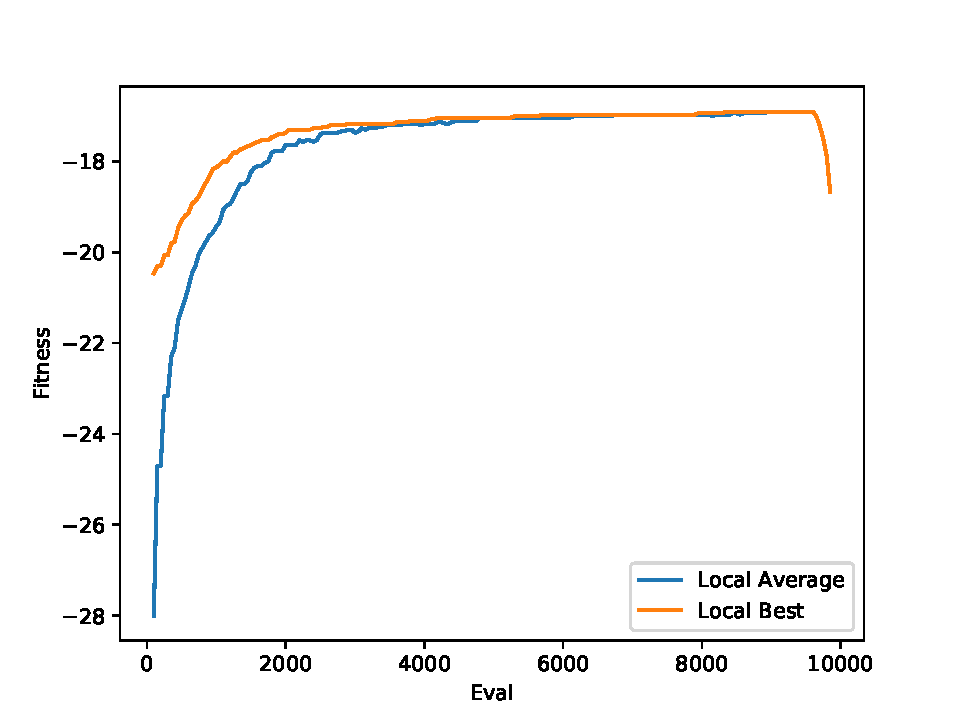
\includegraphics[width=\textwidth]{../graphs/graphs/1016.pdf}
\end{figure}


\begin{table}[!htb]
	\centering
	\caption{Figure \ref{fig:graph_1017} Configuration File}
	\label{tab:graph_1017}
	\begin{tabular}{| c | c |}
		\hline
		Search Algorithm		& EA		 \\
		\hline
		Termination Convergence Criterion		& 10000		 \\
		\hline
		Fitness Evaluations		& 10000		 \\
		\hline
		Survival Strategy		& Plus		 \\
		\hline
		Mutation Algorithm		& Move		 \\
		\hline
		Placement Algorithm		& Random with Penalty		 \\
		\hline
		Tournament Size For Parent Selection		& 5		 \\
		\hline
		Random Seed		& 1017		 \\
		\hline
		Self Adaptive Offspring Count		& False		 \\
		\hline
		Tournament Size For Survival Selection		& 5		 \\
		\hline
		Population Size		& 100		 \\
		\hline
		Survivor Algorithm		& Truncation		 \\
		\hline
		Offspring Count		& 50		 \\
		\hline
		Log File Path		& None		 \\
		\hline
		Penalty Coefficient		& 1		 \\
		\hline
		Parent Selection Algorithm		& k-Tournament Selection with replacement		 \\
		\hline
		Runs		& 30		 \\
		\hline
		Mutation Rate		& 0.1		 \\
		\hline
		Solution File Path		& None		 \\
		\hline
		Recombination Algorithm		& Partially Mapped Crossover		 \\
		\hline
		Self Adaptive Mutation Rate		& False		 \\
		\hline
		Self Adaptive Penalty Coefficient		& False		 \\
		\hline
	\end{tabular}
\end{table}
\begin{figure}[!htb]
	\caption{Input 1}
	\label{fig:graph_1017}
	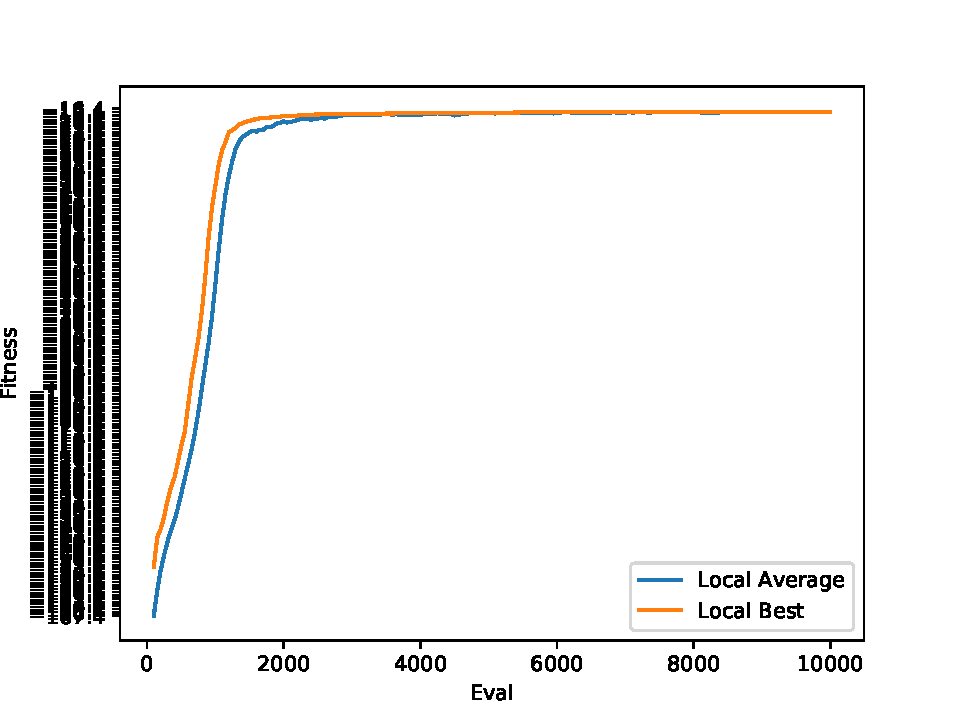
\includegraphics[width=\textwidth]{../graphs/graphs/1017.pdf}
\end{figure}


\begin{table}[!htb]
	\centering
	\caption{Figure \ref{fig:graph_1018} Configuration File}
	\label{tab:graph_1018}
	\begin{tabular}{| c | c |}
		\hline
		Search Algorithm		& EA		 \\
		\hline
		Termination Convergence Criterion		& 10000		 \\
		\hline
		Fitness Evaluations		& 10000		 \\
		\hline
		Survival Strategy		& Plus		 \\
		\hline
		Mutation Algorithm		& Move		 \\
		\hline
		Placement Algorithm		& Random with Penalty		 \\
		\hline
		Tournament Size For Parent Selection		& 5		 \\
		\hline
		Random Seed		& 1018		 \\
		\hline
		Self Adaptive Offspring Count		& True		 \\
		\hline
		Tournament Size For Survival Selection		& 5		 \\
		\hline
		Population Size		& 100		 \\
		\hline
		Survivor Algorithm		& Truncation		 \\
		\hline
		Offspring Count		& 50		 \\
		\hline
		Log File Path		& None		 \\
		\hline
		Penalty Coefficient		& 1		 \\
		\hline
		Parent Selection Algorithm		& k-Tournament Selection with replacement		 \\
		\hline
		Runs		& 30		 \\
		\hline
		Mutation Rate		& 0.1		 \\
		\hline
		Solution File Path		& None		 \\
		\hline
		Recombination Algorithm		& Partially Mapped Crossover		 \\
		\hline
		Self Adaptive Mutation Rate		& False		 \\
		\hline
		Self Adaptive Penalty Coefficient		& False		 \\
		\hline
	\end{tabular}
\end{table}
\begin{figure}[!htb]
	\caption{Input 1}
	\label{fig:graph_1018}
	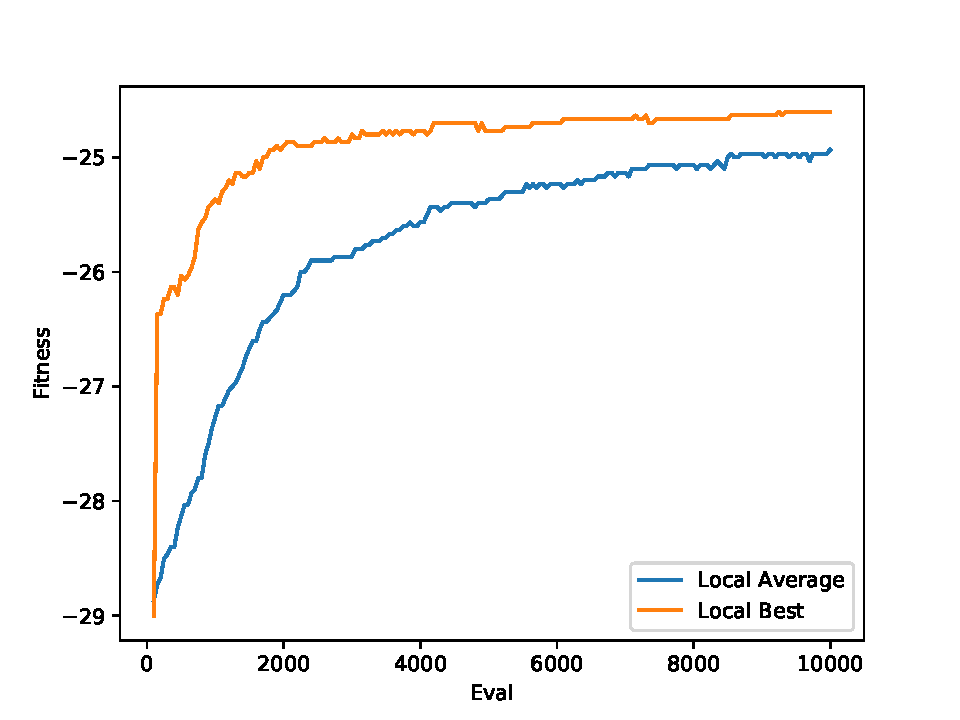
\includegraphics[width=\textwidth]{../graphs/graphs/1018.pdf}
\end{figure}


\begin{table}[!htb]
	\centering
	\caption{Figure \ref{fig:graph_1019} Configuration File}
	\label{tab:graph_1019}
	\begin{tabular}{| c | c |}
		\hline
		Search Algorithm		& EA		 \\
		\hline
		Termination Convergence Criterion		& 10000		 \\
		\hline
		Fitness Evaluations		& 10000		 \\
		\hline
		Survival Strategy		& Plus		 \\
		\hline
		Mutation Algorithm		& Move		 \\
		\hline
		Placement Algorithm		& Random with Penalty		 \\
		\hline
		Tournament Size For Parent Selection		& 5		 \\
		\hline
		Random Seed		& 1019		 \\
		\hline
		Self Adaptive Offspring Count		& False		 \\
		\hline
		Tournament Size For Survival Selection		& 5		 \\
		\hline
		Population Size		& 100		 \\
		\hline
		Survivor Algorithm		& Truncation		 \\
		\hline
		Offspring Count		& 50		 \\
		\hline
		Log File Path		& None		 \\
		\hline
		Penalty Coefficient		& 1		 \\
		\hline
		Parent Selection Algorithm		& k-Tournament Selection with replacement		 \\
		\hline
		Runs		& 30		 \\
		\hline
		Mutation Rate		& 0.1		 \\
		\hline
		Solution File Path		& None		 \\
		\hline
		Recombination Algorithm		& Partially Mapped Crossover		 \\
		\hline
		Self Adaptive Mutation Rate		& False		 \\
		\hline
		Self Adaptive Penalty Coefficient		& True		 \\
		\hline
	\end{tabular}
\end{table}
\begin{figure}[!htb]
	\caption{Input 1}
	\label{fig:graph_1019}
	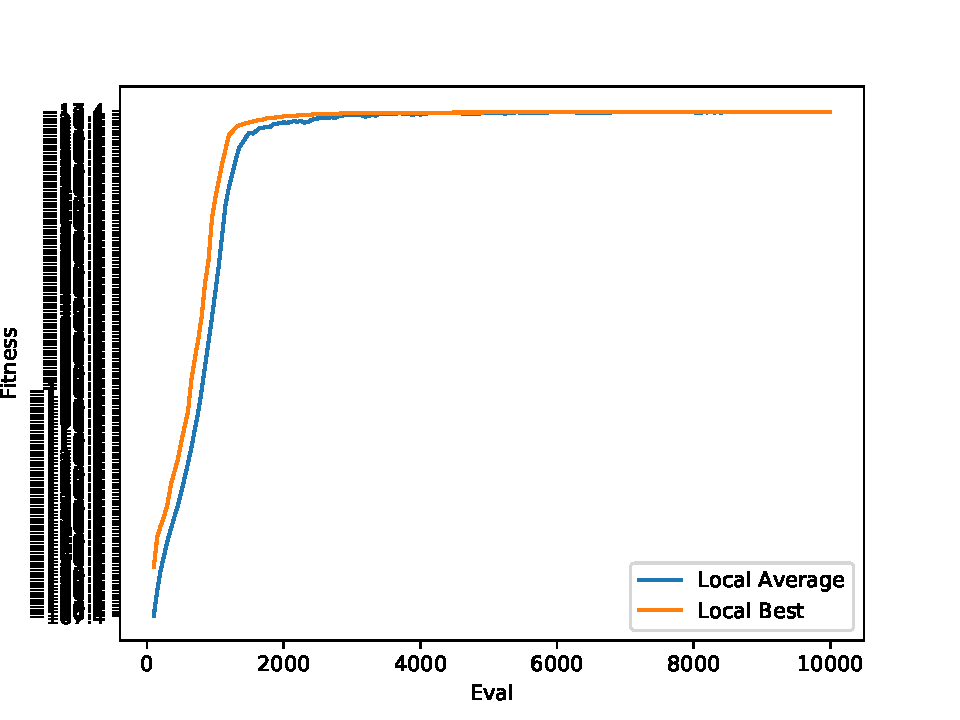
\includegraphics[width=\textwidth]{../graphs/graphs/1019.pdf}
\end{figure}


\begin{table}[!htb]
	\centering
	\caption{Figure \ref{fig:graph_1020} Configuration File}
	\label{tab:graph_1020}
	\begin{tabular}{| c | c |}
		\hline
		Search Algorithm		& EA		 \\
		\hline
		Termination Convergence Criterion		& 10000		 \\
		\hline
		Fitness Evaluations		& 10000		 \\
		\hline
		Survival Strategy		& Plus		 \\
		\hline
		Mutation Algorithm		& Move		 \\
		\hline
		Placement Algorithm		& Random with Penalty		 \\
		\hline
		Tournament Size For Parent Selection		& 5		 \\
		\hline
		Random Seed		& 1020		 \\
		\hline
		Self Adaptive Offspring Count		& True		 \\
		\hline
		Tournament Size For Survival Selection		& 5		 \\
		\hline
		Population Size		& 100		 \\
		\hline
		Survivor Algorithm		& Truncation		 \\
		\hline
		Offspring Count		& 50		 \\
		\hline
		Log File Path		& None		 \\
		\hline
		Penalty Coefficient		& 1		 \\
		\hline
		Parent Selection Algorithm		& k-Tournament Selection with replacement		 \\
		\hline
		Runs		& 30		 \\
		\hline
		Mutation Rate		& 0.1		 \\
		\hline
		Solution File Path		& None		 \\
		\hline
		Recombination Algorithm		& Partially Mapped Crossover		 \\
		\hline
		Self Adaptive Mutation Rate		& False		 \\
		\hline
		Self Adaptive Penalty Coefficient		& True		 \\
		\hline
	\end{tabular}
\end{table}
\begin{figure}[!htb]
	\caption{Input 1}
	\label{fig:graph_1020}
	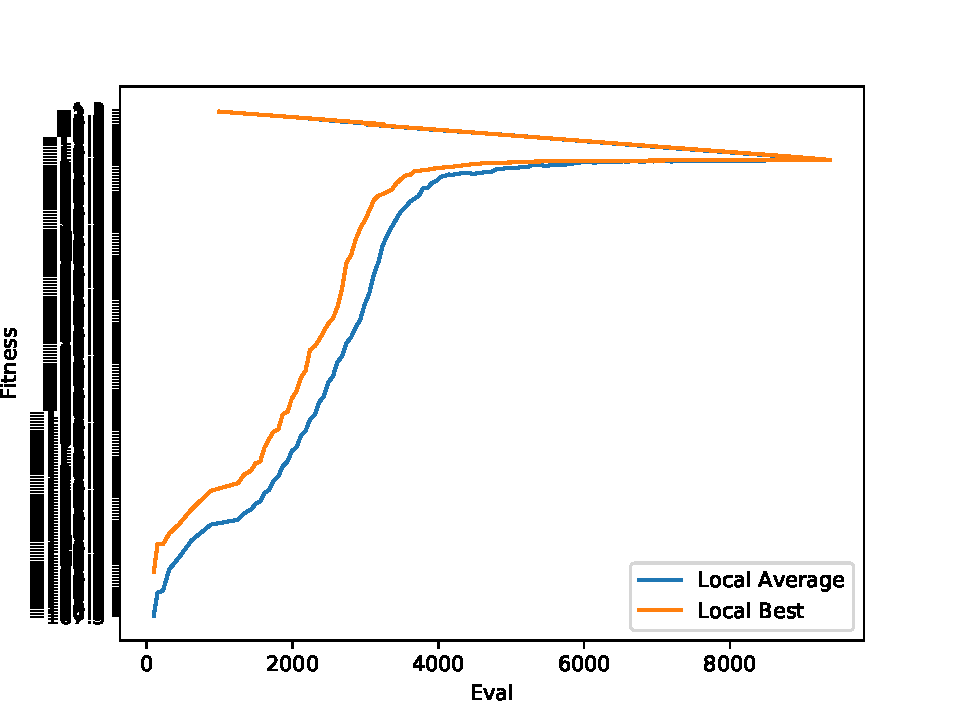
\includegraphics[width=\textwidth]{../graphs/graphs/1020.pdf}
\end{figure}


\clearpage
\begin{table}[!htb]
	\centering
	\caption{Figure \ref{fig:graph_1021} Configuration File}
	\label{tab:graph_1021}
	\begin{tabular}{| c | c |}
		\hline
		Search Algorithm		& EA		 \\
		\hline
		Termination Convergence Criterion		& 10000		 \\
		\hline
		Fitness Evaluations		& 10000		 \\
		\hline
		Survival Strategy		& Plus		 \\
		\hline
		Mutation Algorithm		& Move		 \\
		\hline
		Placement Algorithm		& Random with Penalty		 \\
		\hline
		Tournament Size For Parent Selection		& 5		 \\
		\hline
		Random Seed		& 1021		 \\
		\hline
		Self Adaptive Offspring Count		& False		 \\
		\hline
		Tournament Size For Survival Selection		& 5		 \\
		\hline
		Population Size		& 100		 \\
		\hline
		Survivor Algorithm		& Truncation		 \\
		\hline
		Offspring Count		& 50		 \\
		\hline
		Log File Path		& None		 \\
		\hline
		Penalty Coefficient		& 1		 \\
		\hline
		Parent Selection Algorithm		& k-Tournament Selection with replacement		 \\
		\hline
		Runs		& 30		 \\
		\hline
		Mutation Rate		& 0.1		 \\
		\hline
		Solution File Path		& None		 \\
		\hline
		Recombination Algorithm		& Partially Mapped Crossover		 \\
		\hline
		Self Adaptive Mutation Rate		& True		 \\
		\hline
		Self Adaptive Penalty Coefficient		& False		 \\
		\hline
	\end{tabular}
\end{table}
\begin{figure}[!htb]
	\caption{Input 1}
	\label{fig:graph_1021}
	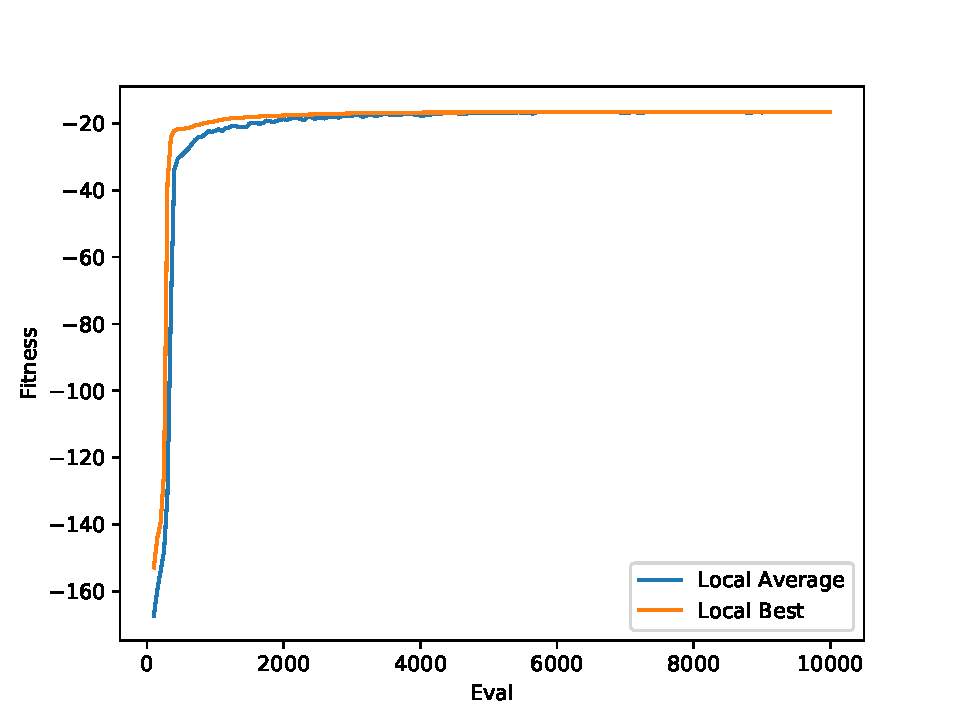
\includegraphics[width=\textwidth]{../graphs/graphs/1021.pdf}
\end{figure}


\begin{table}[!htb]
	\centering
	\caption{Figure \ref{fig:graph_1022} Configuration File}
	\label{tab:graph_1022}
	\begin{tabular}{| c | c |}
		\hline
		Search Algorithm		& EA		 \\
		\hline
		Termination Convergence Criterion		& 10000		 \\
		\hline
		Fitness Evaluations		& 10000		 \\
		\hline
		Survival Strategy		& Plus		 \\
		\hline
		Mutation Algorithm		& Move		 \\
		\hline
		Placement Algorithm		& Random with Penalty		 \\
		\hline
		Tournament Size For Parent Selection		& 5		 \\
		\hline
		Random Seed		& 1022		 \\
		\hline
		Self Adaptive Offspring Count		& True		 \\
		\hline
		Tournament Size For Survival Selection		& 5		 \\
		\hline
		Population Size		& 100		 \\
		\hline
		Survivor Algorithm		& Truncation		 \\
		\hline
		Offspring Count		& 50		 \\
		\hline
		Log File Path		& None		 \\
		\hline
		Penalty Coefficient		& 1		 \\
		\hline
		Parent Selection Algorithm		& k-Tournament Selection with replacement		 \\
		\hline
		Runs		& 30		 \\
		\hline
		Mutation Rate		& 0.1		 \\
		\hline
		Solution File Path		& None		 \\
		\hline
		Recombination Algorithm		& Partially Mapped Crossover		 \\
		\hline
		Self Adaptive Mutation Rate		& True		 \\
		\hline
		Self Adaptive Penalty Coefficient		& False		 \\
		\hline
	\end{tabular}
\end{table}
\begin{figure}[!htb]
	\caption{Input 1}
	\label{fig:graph_1022}
	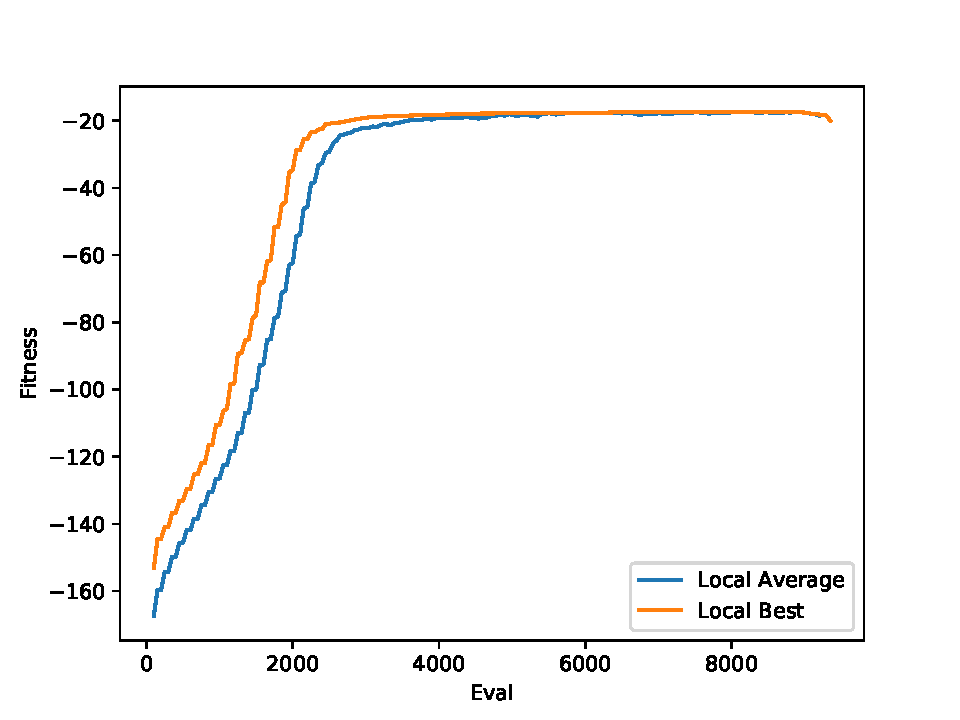
\includegraphics[width=\textwidth]{../graphs/graphs/1022.pdf}
\end{figure}


\begin{table}[!htb]
	\centering
	\caption{Figure \ref{fig:graph_1023} Configuration File}
	\label{tab:graph_1023}
	\begin{tabular}{| c | c |}
		\hline
		Search Algorithm		& EA		 \\
		\hline
		Termination Convergence Criterion		& 10000		 \\
		\hline
		Fitness Evaluations		& 10000		 \\
		\hline
		Survival Strategy		& Plus		 \\
		\hline
		Mutation Algorithm		& Move		 \\
		\hline
		Placement Algorithm		& Random with Penalty		 \\
		\hline
		Tournament Size For Parent Selection		& 5		 \\
		\hline
		Random Seed		& 1023		 \\
		\hline
		Self Adaptive Offspring Count		& False		 \\
		\hline
		Tournament Size For Survival Selection		& 5		 \\
		\hline
		Population Size		& 100		 \\
		\hline
		Survivor Algorithm		& Truncation		 \\
		\hline
		Offspring Count		& 50		 \\
		\hline
		Log File Path		& None		 \\
		\hline
		Penalty Coefficient		& 1		 \\
		\hline
		Parent Selection Algorithm		& k-Tournament Selection with replacement		 \\
		\hline
		Runs		& 30		 \\
		\hline
		Mutation Rate		& 0.1		 \\
		\hline
		Solution File Path		& None		 \\
		\hline
		Recombination Algorithm		& Partially Mapped Crossover		 \\
		\hline
		Self Adaptive Mutation Rate		& True		 \\
		\hline
		Self Adaptive Penalty Coefficient		& True		 \\
		\hline
	\end{tabular}
\end{table}
\begin{figure}[!htb]
	\caption{Input 1}
	\label{fig:graph_1023}
	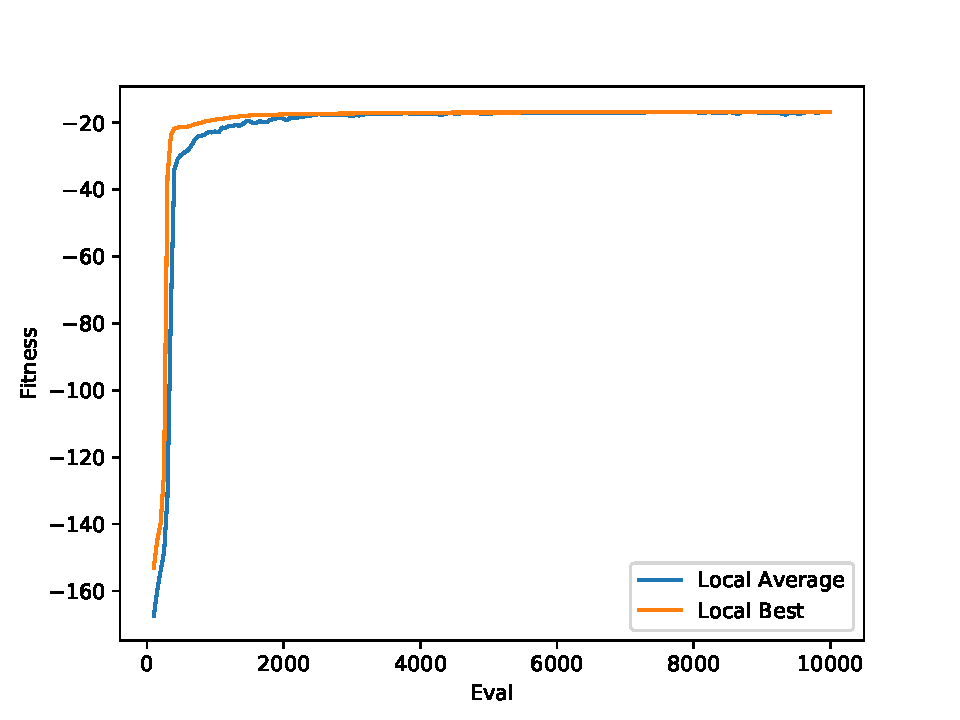
\includegraphics[width=\textwidth]{../graphs/graphs/1023.pdf}
\end{figure}


\begin{table}[!htb]
	\centering
	\caption{Figure \ref{fig:graph_1024} Configuration File}
	\label{tab:graph_1024}
	\begin{tabular}{| c | c |}
		\hline
		Search Algorithm		& EA		 \\
		\hline
		Termination Convergence Criterion		& 10000		 \\
		\hline
		Fitness Evaluations		& 10000		 \\
		\hline
		Survival Strategy		& Plus		 \\
		\hline
		Mutation Algorithm		& Move		 \\
		\hline
		Placement Algorithm		& Random with Penalty		 \\
		\hline
		Tournament Size For Parent Selection		& 5		 \\
		\hline
		Random Seed		& 1024		 \\
		\hline
		Self Adaptive Offspring Count		& True		 \\
		\hline
		Tournament Size For Survival Selection		& 5		 \\
		\hline
		Population Size		& 100		 \\
		\hline
		Survivor Algorithm		& Truncation		 \\
		\hline
		Offspring Count		& 50		 \\
		\hline
		Log File Path		& None		 \\
		\hline
		Penalty Coefficient		& 1		 \\
		\hline
		Parent Selection Algorithm		& k-Tournament Selection with replacement		 \\
		\hline
		Runs		& 30		 \\
		\hline
		Mutation Rate		& 0.1		 \\
		\hline
		Solution File Path		& None		 \\
		\hline
		Recombination Algorithm		& Partially Mapped Crossover		 \\
		\hline
		Self Adaptive Mutation Rate		& True		 \\
		\hline
		Self Adaptive Penalty Coefficient		& True		 \\
		\hline
	\end{tabular}
\end{table}
\begin{figure}[!htb]
	\caption{Input 1}
	\label{fig:graph_1024}
	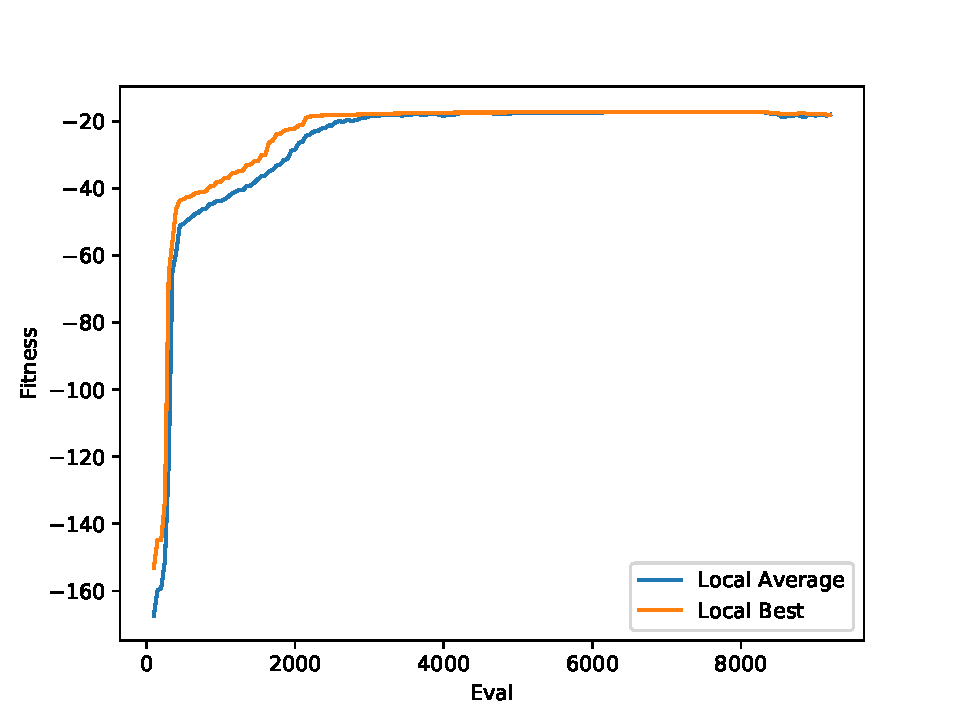
\includegraphics[width=\textwidth]{../graphs/graphs/1024.pdf}
\end{figure}


\begin{table}[!htb]
	\centering
	\caption{Figure \ref{fig:graph_1025} Configuration File}
	\label{tab:graph_1025}
	\begin{tabular}{| c | c |}
		\hline
		Search Algorithm		& EA		 \\
		\hline
		Termination Convergence Criterion		& 10000		 \\
		\hline
		Fitness Evaluations		& 10000		 \\
		\hline
		Survival Strategy		& Plus		 \\
		\hline
		Mutation Algorithm		& Flip		 \\
		\hline
		Placement Algorithm		& Random		 \\
		\hline
		Tournament Size For Parent Selection		& 5		 \\
		\hline
		Random Seed		& 1025		 \\
		\hline
		Self Adaptive Offspring Count		& False		 \\
		\hline
		Tournament Size For Survival Selection		& 5		 \\
		\hline
		Population Size		& 100		 \\
		\hline
		Survivor Algorithm		& Truncation		 \\
		\hline
		Offspring Count		& 50		 \\
		\hline
		Log File Path		& None		 \\
		\hline
		Penalty Coefficient		& 1		 \\
		\hline
		Parent Selection Algorithm		& k-Tournament Selection with replacement		 \\
		\hline
		Runs		& 30		 \\
		\hline
		Mutation Rate		& 0.1		 \\
		\hline
		Solution File Path		& None		 \\
		\hline
		Recombination Algorithm		& Partially Mapped Crossover		 \\
		\hline
		Self Adaptive Mutation Rate		& False		 \\
		\hline
		Self Adaptive Penalty Coefficient		& False		 \\
		\hline
	\end{tabular}
\end{table}
\begin{figure}[!htb]
	\caption{Input 1}
	\label{fig:graph_1025}
	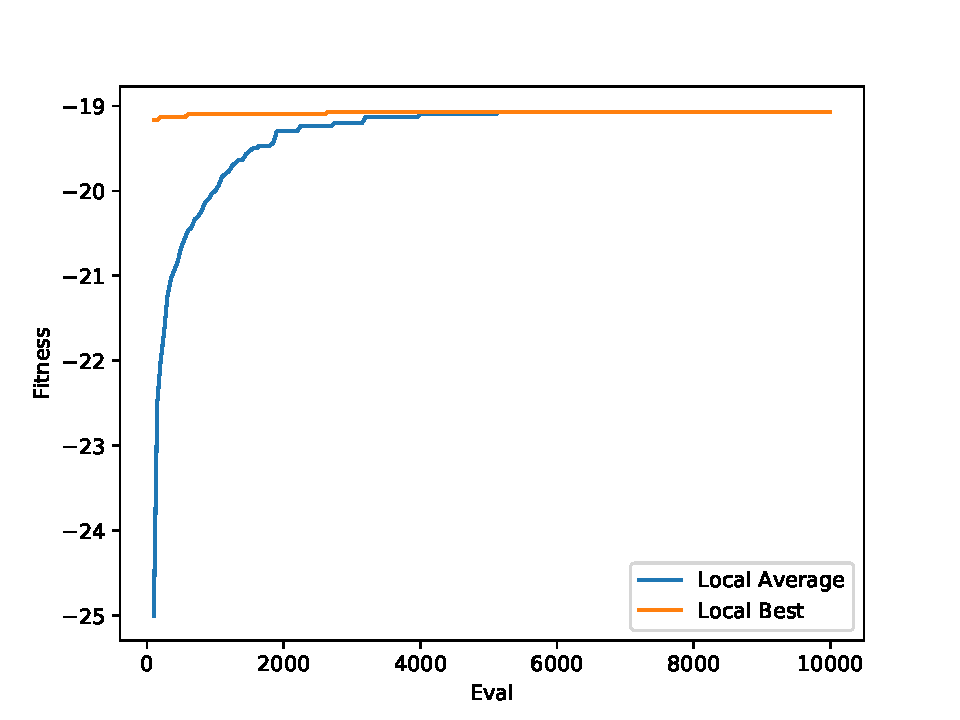
\includegraphics[width=\textwidth]{../graphs/graphs/1025.pdf}
\end{figure}


\begin{table}[!htb]
	\centering
	\caption{Figure \ref{fig:graph_1026} Configuration File}
	\label{tab:graph_1026}
	\begin{tabular}{| c | c |}
		\hline
		Search Algorithm		& EA		 \\
		\hline
		Termination Convergence Criterion		& 10000		 \\
		\hline
		Fitness Evaluations		& 10000		 \\
		\hline
		Survival Strategy		& Plus		 \\
		\hline
		Mutation Algorithm		& Flip		 \\
		\hline
		Placement Algorithm		& Random		 \\
		\hline
		Tournament Size For Parent Selection		& 5		 \\
		\hline
		Random Seed		& 1026		 \\
		\hline
		Self Adaptive Offspring Count		& True		 \\
		\hline
		Tournament Size For Survival Selection		& 5		 \\
		\hline
		Population Size		& 100		 \\
		\hline
		Survivor Algorithm		& Truncation		 \\
		\hline
		Offspring Count		& 50		 \\
		\hline
		Log File Path		& None		 \\
		\hline
		Penalty Coefficient		& 1		 \\
		\hline
		Parent Selection Algorithm		& k-Tournament Selection with replacement		 \\
		\hline
		Runs		& 30		 \\
		\hline
		Mutation Rate		& 0.1		 \\
		\hline
		Solution File Path		& None		 \\
		\hline
		Recombination Algorithm		& Partially Mapped Crossover		 \\
		\hline
		Self Adaptive Mutation Rate		& False		 \\
		\hline
		Self Adaptive Penalty Coefficient		& False		 \\
		\hline
	\end{tabular}
\end{table}
\begin{figure}[!htb]
	\caption{Input 1}
	\label{fig:graph_1026}
	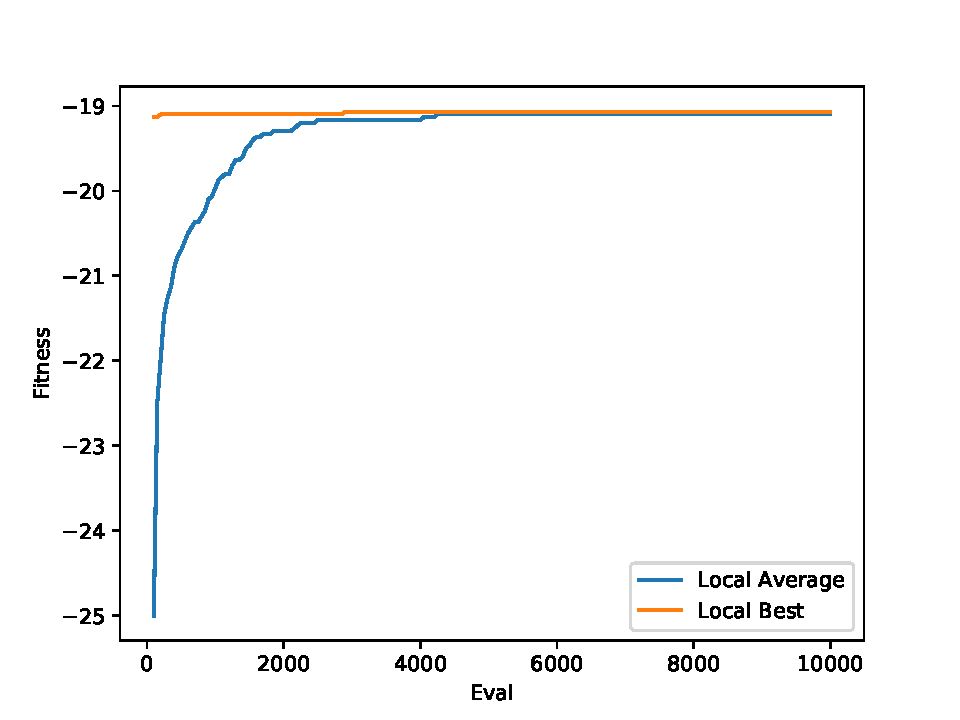
\includegraphics[width=\textwidth]{../graphs/graphs/1026.pdf}
\end{figure}


\begin{table}[!htb]
	\centering
	\caption{Figure \ref{fig:graph_1027} Configuration File}
	\label{tab:graph_1027}
	\begin{tabular}{| c | c |}
		\hline
		Search Algorithm		& EA		 \\
		\hline
		Termination Convergence Criterion		& 10000		 \\
		\hline
		Fitness Evaluations		& 10000		 \\
		\hline
		Survival Strategy		& Plus		 \\
		\hline
		Mutation Algorithm		& Flip		 \\
		\hline
		Placement Algorithm		& Random		 \\
		\hline
		Tournament Size For Parent Selection		& 5		 \\
		\hline
		Random Seed		& 1027		 \\
		\hline
		Self Adaptive Offspring Count		& False		 \\
		\hline
		Tournament Size For Survival Selection		& 5		 \\
		\hline
		Population Size		& 100		 \\
		\hline
		Survivor Algorithm		& Truncation		 \\
		\hline
		Offspring Count		& 50		 \\
		\hline
		Log File Path		& None		 \\
		\hline
		Penalty Coefficient		& 1		 \\
		\hline
		Parent Selection Algorithm		& k-Tournament Selection with replacement		 \\
		\hline
		Runs		& 30		 \\
		\hline
		Mutation Rate		& 0.1		 \\
		\hline
		Solution File Path		& None		 \\
		\hline
		Recombination Algorithm		& Partially Mapped Crossover		 \\
		\hline
		Self Adaptive Mutation Rate		& False		 \\
		\hline
		Self Adaptive Penalty Coefficient		& True		 \\
		\hline
	\end{tabular}
\end{table}
\begin{figure}[!htb]
	\caption{Input 1}
	\label{fig:graph_1027}
	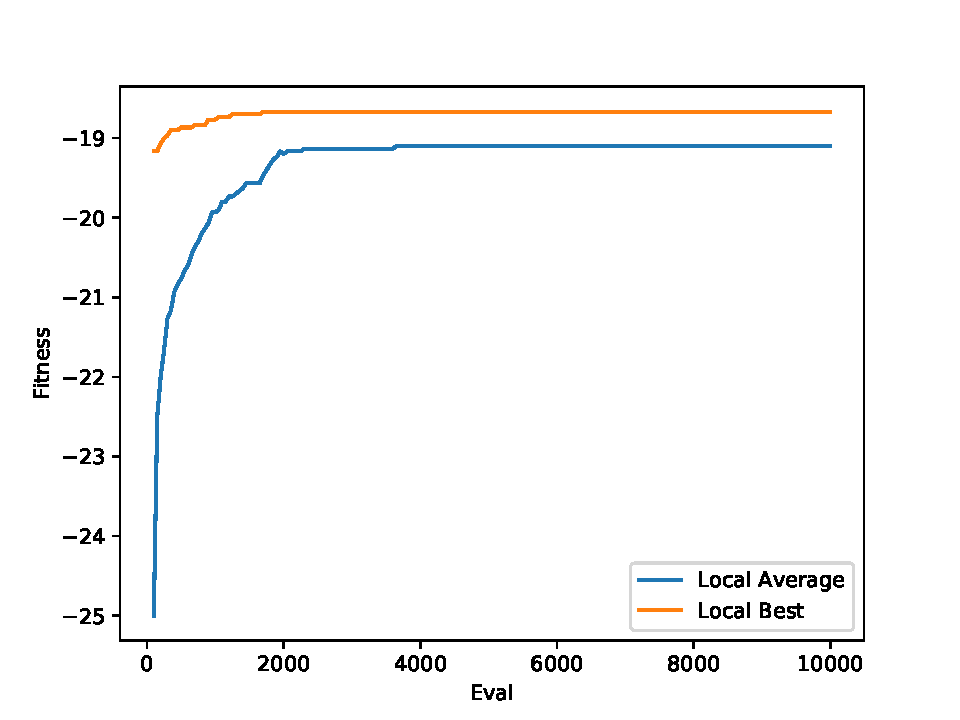
\includegraphics[width=\textwidth]{../graphs/graphs/1027.pdf}
\end{figure}


\begin{table}[!htb]
	\centering
	\caption{Figure \ref{fig:graph_1028} Configuration File}
	\label{tab:graph_1028}
	\begin{tabular}{| c | c |}
		\hline
		Search Algorithm		& EA		 \\
		\hline
		Termination Convergence Criterion		& 10000		 \\
		\hline
		Fitness Evaluations		& 10000		 \\
		\hline
		Survival Strategy		& Plus		 \\
		\hline
		Mutation Algorithm		& Flip		 \\
		\hline
		Placement Algorithm		& Random		 \\
		\hline
		Tournament Size For Parent Selection		& 5		 \\
		\hline
		Random Seed		& 1028		 \\
		\hline
		Self Adaptive Offspring Count		& True		 \\
		\hline
		Tournament Size For Survival Selection		& 5		 \\
		\hline
		Population Size		& 100		 \\
		\hline
		Survivor Algorithm		& Truncation		 \\
		\hline
		Offspring Count		& 50		 \\
		\hline
		Log File Path		& None		 \\
		\hline
		Penalty Coefficient		& 1		 \\
		\hline
		Parent Selection Algorithm		& k-Tournament Selection with replacement		 \\
		\hline
		Runs		& 30		 \\
		\hline
		Mutation Rate		& 0.1		 \\
		\hline
		Solution File Path		& None		 \\
		\hline
		Recombination Algorithm		& Partially Mapped Crossover		 \\
		\hline
		Self Adaptive Mutation Rate		& False		 \\
		\hline
		Self Adaptive Penalty Coefficient		& True		 \\
		\hline
	\end{tabular}
\end{table}
\begin{figure}[!htb]
	\caption{Input 1}
	\label{fig:graph_1028}
	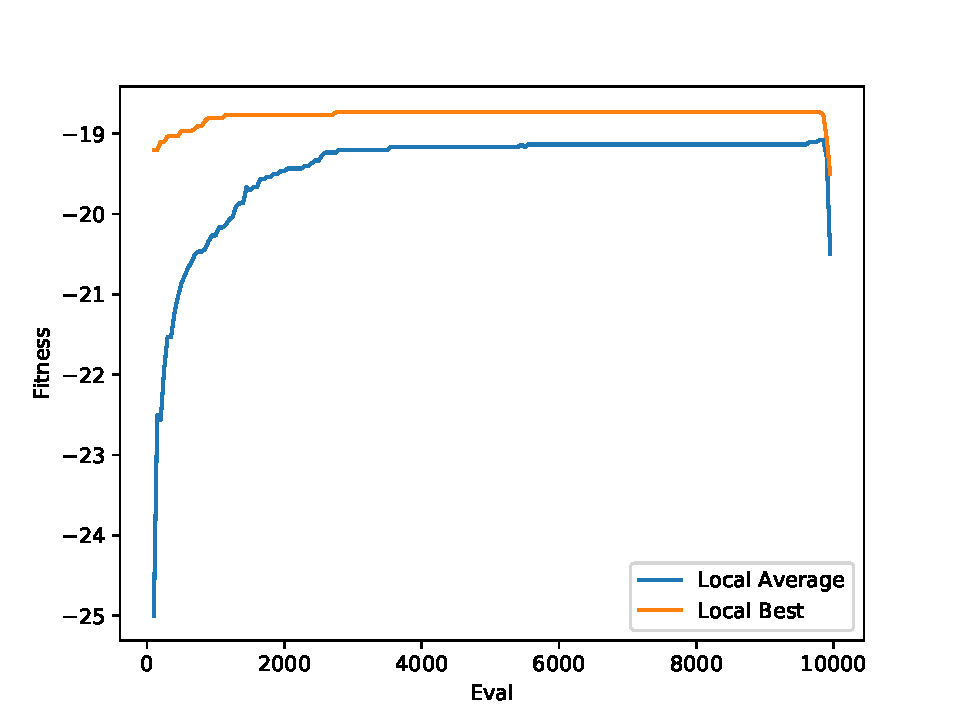
\includegraphics[width=\textwidth]{../graphs/graphs/1028.pdf}
\end{figure}


\begin{table}[!htb]
	\centering
	\caption{Figure \ref{fig:graph_1029} Configuration File}
	\label{tab:graph_1029}
	\begin{tabular}{| c | c |}
		\hline
		Search Algorithm		& EA		 \\
		\hline
		Termination Convergence Criterion		& 10000		 \\
		\hline
		Fitness Evaluations		& 10000		 \\
		\hline
		Survival Strategy		& Plus		 \\
		\hline
		Mutation Algorithm		& Flip		 \\
		\hline
		Placement Algorithm		& Random		 \\
		\hline
		Tournament Size For Parent Selection		& 5		 \\
		\hline
		Random Seed		& 1029		 \\
		\hline
		Self Adaptive Offspring Count		& False		 \\
		\hline
		Tournament Size For Survival Selection		& 5		 \\
		\hline
		Population Size		& 100		 \\
		\hline
		Survivor Algorithm		& Truncation		 \\
		\hline
		Offspring Count		& 50		 \\
		\hline
		Log File Path		& None		 \\
		\hline
		Penalty Coefficient		& 1		 \\
		\hline
		Parent Selection Algorithm		& k-Tournament Selection with replacement		 \\
		\hline
		Runs		& 30		 \\
		\hline
		Mutation Rate		& 0.1		 \\
		\hline
		Solution File Path		& None		 \\
		\hline
		Recombination Algorithm		& Partially Mapped Crossover		 \\
		\hline
		Self Adaptive Mutation Rate		& True		 \\
		\hline
		Self Adaptive Penalty Coefficient		& False		 \\
		\hline
	\end{tabular}
\end{table}
\begin{figure}[!htb]
	\caption{Input 1}
	\label{fig:graph_1029}
	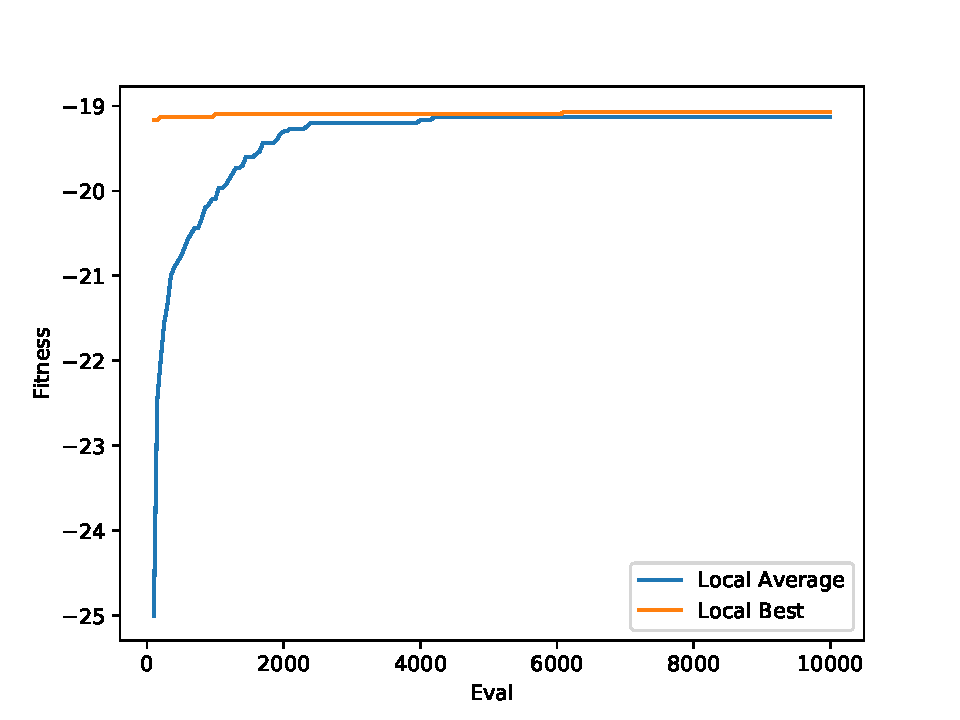
\includegraphics[width=\textwidth]{../graphs/graphs/1029.pdf}
\end{figure}


\begin{table}[!htb]
	\centering
	\caption{Figure \ref{fig:graph_1030} Configuration File}
	\label{tab:graph_1030}
	\begin{tabular}{| c | c |}
		\hline
		Search Algorithm		& EA		 \\
		\hline
		Termination Convergence Criterion		& 10000		 \\
		\hline
		Fitness Evaluations		& 10000		 \\
		\hline
		Survival Strategy		& Plus		 \\
		\hline
		Mutation Algorithm		& Flip		 \\
		\hline
		Placement Algorithm		& Random		 \\
		\hline
		Tournament Size For Parent Selection		& 5		 \\
		\hline
		Random Seed		& 1030		 \\
		\hline
		Self Adaptive Offspring Count		& True		 \\
		\hline
		Tournament Size For Survival Selection		& 5		 \\
		\hline
		Population Size		& 100		 \\
		\hline
		Survivor Algorithm		& Truncation		 \\
		\hline
		Offspring Count		& 50		 \\
		\hline
		Log File Path		& None		 \\
		\hline
		Penalty Coefficient		& 1		 \\
		\hline
		Parent Selection Algorithm		& k-Tournament Selection with replacement		 \\
		\hline
		Runs		& 30		 \\
		\hline
		Mutation Rate		& 0.1		 \\
		\hline
		Solution File Path		& None		 \\
		\hline
		Recombination Algorithm		& Partially Mapped Crossover		 \\
		\hline
		Self Adaptive Mutation Rate		& True		 \\
		\hline
		Self Adaptive Penalty Coefficient		& False		 \\
		\hline
	\end{tabular}
\end{table}
\begin{figure}[!htb]
	\caption{Input 1}
	\label{fig:graph_1030}
	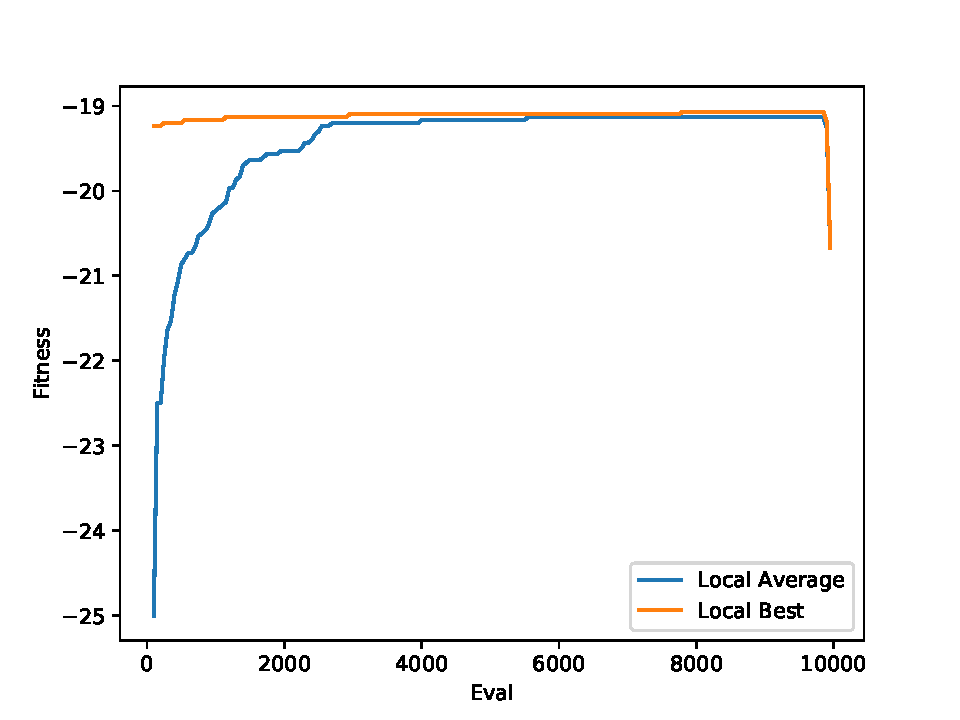
\includegraphics[width=\textwidth]{../graphs/graphs/1030.pdf}
\end{figure}


\clearpage
\begin{table}[!htb]
	\centering
	\caption{Figure \ref{fig:graph_1031} Configuration File}
	\label{tab:graph_1031}
	\begin{tabular}{| c | c |}
		\hline
		Search Algorithm		& EA		 \\
		\hline
		Termination Convergence Criterion		& 10000		 \\
		\hline
		Fitness Evaluations		& 10000		 \\
		\hline
		Survival Strategy		& Plus		 \\
		\hline
		Mutation Algorithm		& Flip		 \\
		\hline
		Placement Algorithm		& Random		 \\
		\hline
		Tournament Size For Parent Selection		& 5		 \\
		\hline
		Random Seed		& 1031		 \\
		\hline
		Self Adaptive Offspring Count		& False		 \\
		\hline
		Tournament Size For Survival Selection		& 5		 \\
		\hline
		Population Size		& 100		 \\
		\hline
		Survivor Algorithm		& Truncation		 \\
		\hline
		Offspring Count		& 50		 \\
		\hline
		Log File Path		& None		 \\
		\hline
		Penalty Coefficient		& 1		 \\
		\hline
		Parent Selection Algorithm		& k-Tournament Selection with replacement		 \\
		\hline
		Runs		& 30		 \\
		\hline
		Mutation Rate		& 0.1		 \\
		\hline
		Solution File Path		& None		 \\
		\hline
		Recombination Algorithm		& Partially Mapped Crossover		 \\
		\hline
		Self Adaptive Mutation Rate		& True		 \\
		\hline
		Self Adaptive Penalty Coefficient		& True		 \\
		\hline
	\end{tabular}
\end{table}
\begin{figure}[!htb]
	\caption{Input 1}
	\label{fig:graph_1031}
	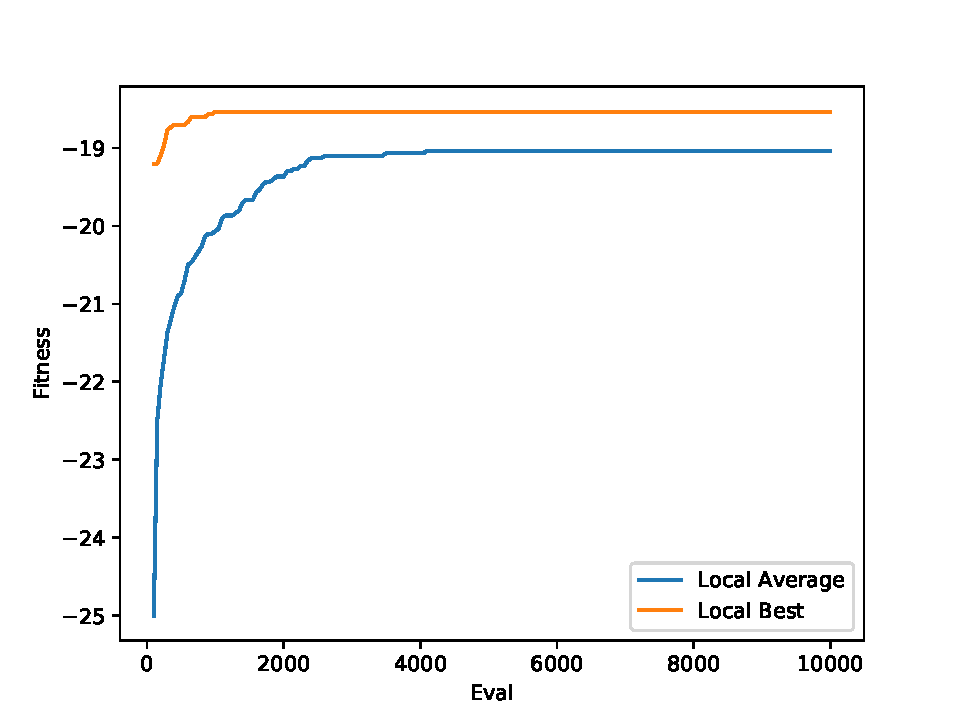
\includegraphics[width=\textwidth]{../graphs/graphs/1031.pdf}
\end{figure}


\begin{table}[!htb]
	\centering
	\caption{Figure \ref{fig:graph_1032} Configuration File}
	\label{tab:graph_1032}
	\begin{tabular}{| c | c |}
		\hline
		Search Algorithm		& EA		 \\
		\hline
		Termination Convergence Criterion		& 10000		 \\
		\hline
		Fitness Evaluations		& 10000		 \\
		\hline
		Survival Strategy		& Plus		 \\
		\hline
		Mutation Algorithm		& Flip		 \\
		\hline
		Placement Algorithm		& Random		 \\
		\hline
		Tournament Size For Parent Selection		& 5		 \\
		\hline
		Random Seed		& 1032		 \\
		\hline
		Self Adaptive Offspring Count		& True		 \\
		\hline
		Tournament Size For Survival Selection		& 5		 \\
		\hline
		Population Size		& 100		 \\
		\hline
		Survivor Algorithm		& Truncation		 \\
		\hline
		Offspring Count		& 50		 \\
		\hline
		Log File Path		& None		 \\
		\hline
		Penalty Coefficient		& 1		 \\
		\hline
		Parent Selection Algorithm		& k-Tournament Selection with replacement		 \\
		\hline
		Runs		& 30		 \\
		\hline
		Mutation Rate		& 0.1		 \\
		\hline
		Solution File Path		& None		 \\
		\hline
		Recombination Algorithm		& Partially Mapped Crossover		 \\
		\hline
		Self Adaptive Mutation Rate		& True		 \\
		\hline
		Self Adaptive Penalty Coefficient		& True		 \\
		\hline
	\end{tabular}
\end{table}
\begin{figure}[!htb]
	\caption{Input 1}
	\label{fig:graph_1032}
	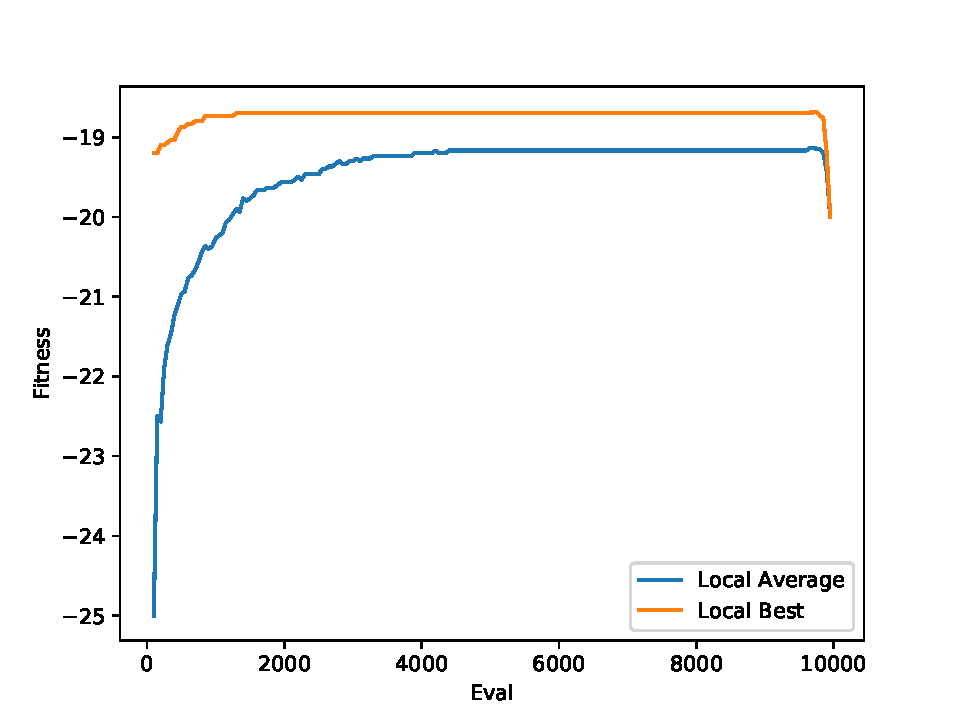
\includegraphics[width=\textwidth]{../graphs/graphs/1032.pdf}
\end{figure}


\begin{table}[!htb]
	\centering
	\caption{Figure \ref{fig:graph_1033} Configuration File}
	\label{tab:graph_1033}
	\begin{tabular}{| c | c |}
		\hline
		Search Algorithm		& EA		 \\
		\hline
		Termination Convergence Criterion		& 10000		 \\
		\hline
		Fitness Evaluations		& 10000		 \\
		\hline
		Survival Strategy		& Plus		 \\
		\hline
		Mutation Algorithm		& Flip		 \\
		\hline
		Placement Algorithm		& Random with Repair		 \\
		\hline
		Tournament Size For Parent Selection		& 5		 \\
		\hline
		Random Seed		& 1033		 \\
		\hline
		Self Adaptive Offspring Count		& False		 \\
		\hline
		Tournament Size For Survival Selection		& 5		 \\
		\hline
		Population Size		& 100		 \\
		\hline
		Survivor Algorithm		& Truncation		 \\
		\hline
		Offspring Count		& 50		 \\
		\hline
		Log File Path		& None		 \\
		\hline
		Penalty Coefficient		& 1		 \\
		\hline
		Parent Selection Algorithm		& k-Tournament Selection with replacement		 \\
		\hline
		Runs		& 30		 \\
		\hline
		Mutation Rate		& 0.1		 \\
		\hline
		Solution File Path		& None		 \\
		\hline
		Recombination Algorithm		& Partially Mapped Crossover		 \\
		\hline
		Self Adaptive Mutation Rate		& False		 \\
		\hline
		Self Adaptive Penalty Coefficient		& False		 \\
		\hline
	\end{tabular}
\end{table}
\begin{figure}[!htb]
	\caption{Input 1}
	\label{fig:graph_1033}
	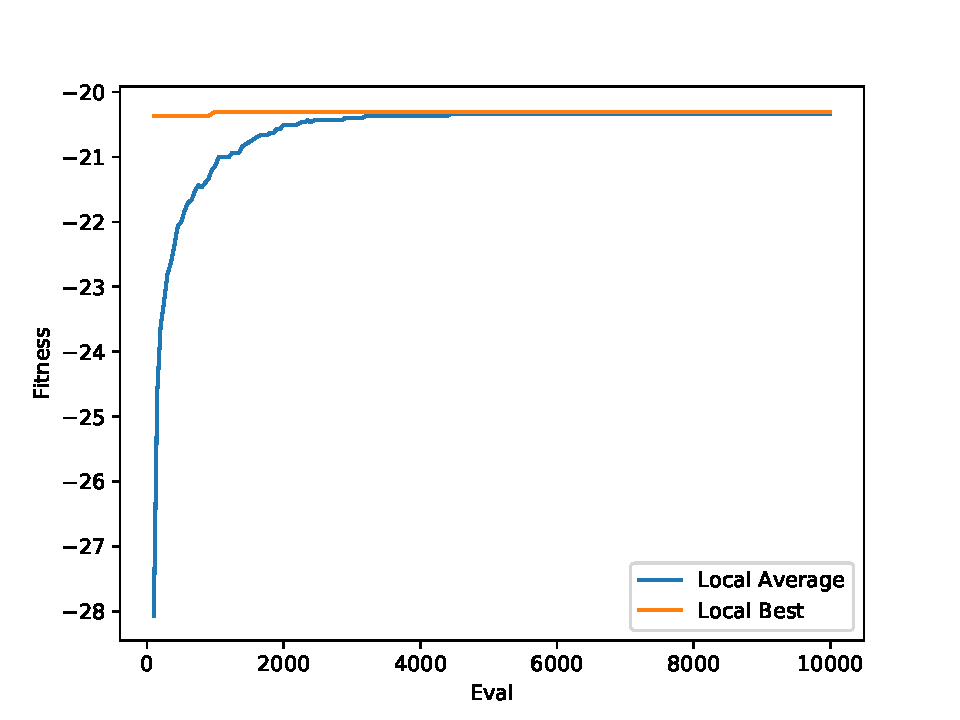
\includegraphics[width=\textwidth]{../graphs/graphs/1033.pdf}
\end{figure}


\begin{table}[!htb]
	\centering
	\caption{Figure \ref{fig:graph_1034} Configuration File}
	\label{tab:graph_1034}
	\begin{tabular}{| c | c |}
		\hline
		Search Algorithm		& EA		 \\
		\hline
		Termination Convergence Criterion		& 10000		 \\
		\hline
		Fitness Evaluations		& 10000		 \\
		\hline
		Survival Strategy		& Plus		 \\
		\hline
		Mutation Algorithm		& Flip		 \\
		\hline
		Placement Algorithm		& Random with Repair		 \\
		\hline
		Tournament Size For Parent Selection		& 5		 \\
		\hline
		Random Seed		& 1034		 \\
		\hline
		Self Adaptive Offspring Count		& True		 \\
		\hline
		Tournament Size For Survival Selection		& 5		 \\
		\hline
		Population Size		& 100		 \\
		\hline
		Survivor Algorithm		& Truncation		 \\
		\hline
		Offspring Count		& 50		 \\
		\hline
		Log File Path		& None		 \\
		\hline
		Penalty Coefficient		& 1		 \\
		\hline
		Parent Selection Algorithm		& k-Tournament Selection with replacement		 \\
		\hline
		Runs		& 30		 \\
		\hline
		Mutation Rate		& 0.1		 \\
		\hline
		Solution File Path		& None		 \\
		\hline
		Recombination Algorithm		& Partially Mapped Crossover		 \\
		\hline
		Self Adaptive Mutation Rate		& False		 \\
		\hline
		Self Adaptive Penalty Coefficient		& False		 \\
		\hline
	\end{tabular}
\end{table}
\begin{figure}[!htb]
	\caption{Input 1}
	\label{fig:graph_1034}
	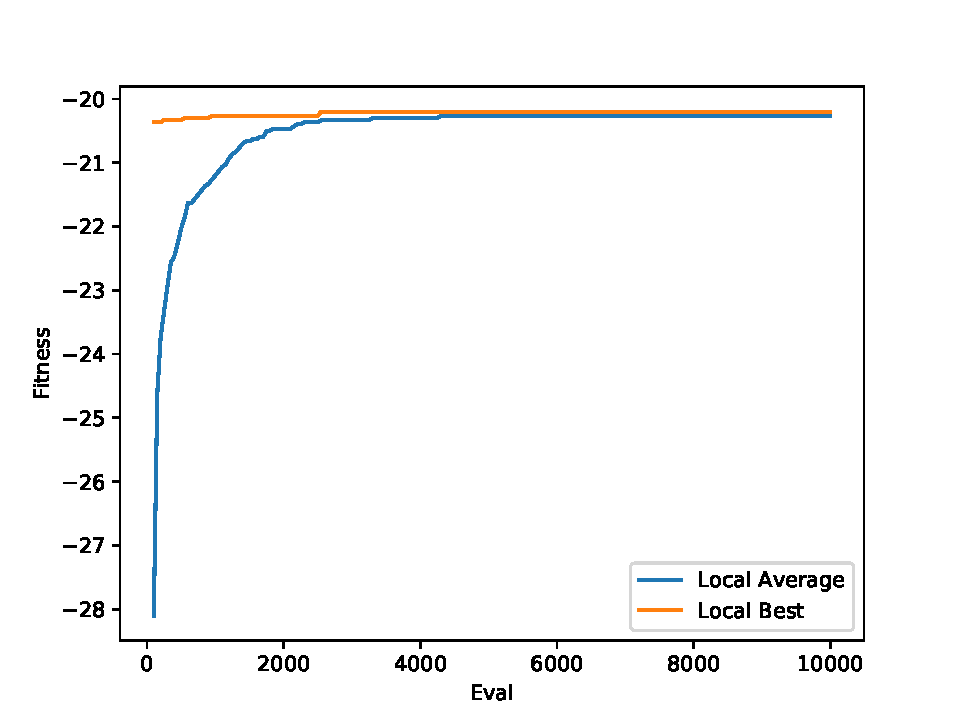
\includegraphics[width=\textwidth]{../graphs/graphs/1034.pdf}
\end{figure}


\begin{table}[!htb]
	\centering
	\caption{Figure \ref{fig:graph_1035} Configuration File}
	\label{tab:graph_1035}
	\begin{tabular}{| c | c |}
		\hline
		Search Algorithm		& EA		 \\
		\hline
		Termination Convergence Criterion		& 10000		 \\
		\hline
		Fitness Evaluations		& 10000		 \\
		\hline
		Survival Strategy		& Plus		 \\
		\hline
		Mutation Algorithm		& Flip		 \\
		\hline
		Placement Algorithm		& Random with Repair		 \\
		\hline
		Tournament Size For Parent Selection		& 5		 \\
		\hline
		Random Seed		& 1035		 \\
		\hline
		Self Adaptive Offspring Count		& False		 \\
		\hline
		Tournament Size For Survival Selection		& 5		 \\
		\hline
		Population Size		& 100		 \\
		\hline
		Survivor Algorithm		& Truncation		 \\
		\hline
		Offspring Count		& 50		 \\
		\hline
		Log File Path		& None		 \\
		\hline
		Penalty Coefficient		& 1		 \\
		\hline
		Parent Selection Algorithm		& k-Tournament Selection with replacement		 \\
		\hline
		Runs		& 30		 \\
		\hline
		Mutation Rate		& 0.1		 \\
		\hline
		Solution File Path		& None		 \\
		\hline
		Recombination Algorithm		& Partially Mapped Crossover		 \\
		\hline
		Self Adaptive Mutation Rate		& False		 \\
		\hline
		Self Adaptive Penalty Coefficient		& True		 \\
		\hline
	\end{tabular}
\end{table}
\begin{figure}[!htb]
	\caption{Input 1}
	\label{fig:graph_1035}
	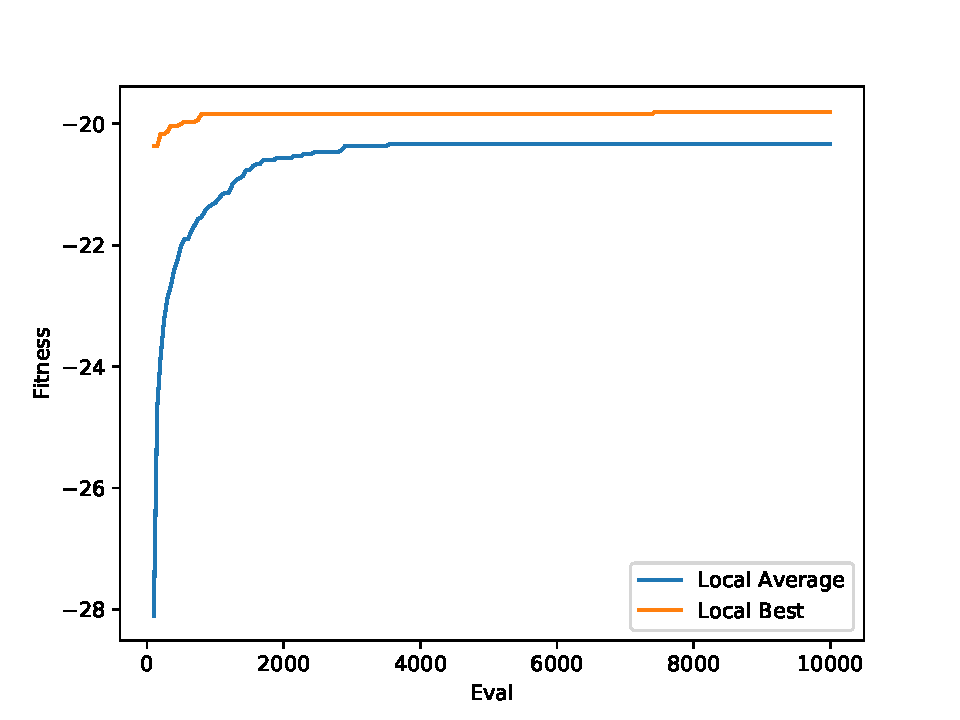
\includegraphics[width=\textwidth]{../graphs/graphs/1035.pdf}
\end{figure}


\begin{table}[!htb]
	\centering
	\caption{Figure \ref{fig:graph_1036} Configuration File}
	\label{tab:graph_1036}
	\begin{tabular}{| c | c |}
		\hline
		Search Algorithm		& EA		 \\
		\hline
		Termination Convergence Criterion		& 10000		 \\
		\hline
		Fitness Evaluations		& 10000		 \\
		\hline
		Survival Strategy		& Plus		 \\
		\hline
		Mutation Algorithm		& Flip		 \\
		\hline
		Placement Algorithm		& Random with Repair		 \\
		\hline
		Tournament Size For Parent Selection		& 5		 \\
		\hline
		Random Seed		& 1036		 \\
		\hline
		Self Adaptive Offspring Count		& True		 \\
		\hline
		Tournament Size For Survival Selection		& 5		 \\
		\hline
		Population Size		& 100		 \\
		\hline
		Survivor Algorithm		& Truncation		 \\
		\hline
		Offspring Count		& 50		 \\
		\hline
		Log File Path		& None		 \\
		\hline
		Penalty Coefficient		& 1		 \\
		\hline
		Parent Selection Algorithm		& k-Tournament Selection with replacement		 \\
		\hline
		Runs		& 30		 \\
		\hline
		Mutation Rate		& 0.1		 \\
		\hline
		Solution File Path		& None		 \\
		\hline
		Recombination Algorithm		& Partially Mapped Crossover		 \\
		\hline
		Self Adaptive Mutation Rate		& False		 \\
		\hline
		Self Adaptive Penalty Coefficient		& True		 \\
		\hline
	\end{tabular}
\end{table}
\begin{figure}[!htb]
	\caption{Input 1}
	\label{fig:graph_1036}
	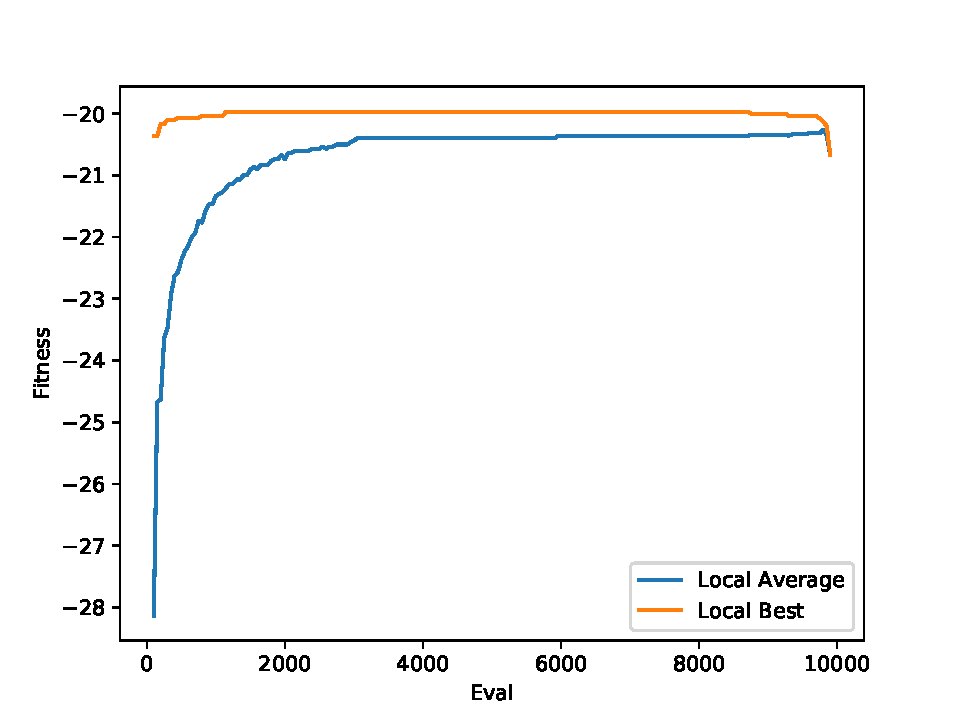
\includegraphics[width=\textwidth]{../graphs/graphs/1036.pdf}
\end{figure}


\begin{table}[!htb]
	\centering
	\caption{Figure \ref{fig:graph_1037} Configuration File}
	\label{tab:graph_1037}
	\begin{tabular}{| c | c |}
		\hline
		Search Algorithm		& EA		 \\
		\hline
		Termination Convergence Criterion		& 10000		 \\
		\hline
		Fitness Evaluations		& 10000		 \\
		\hline
		Survival Strategy		& Plus		 \\
		\hline
		Mutation Algorithm		& Flip		 \\
		\hline
		Placement Algorithm		& Random with Repair		 \\
		\hline
		Tournament Size For Parent Selection		& 5		 \\
		\hline
		Random Seed		& 1037		 \\
		\hline
		Self Adaptive Offspring Count		& False		 \\
		\hline
		Tournament Size For Survival Selection		& 5		 \\
		\hline
		Population Size		& 100		 \\
		\hline
		Survivor Algorithm		& Truncation		 \\
		\hline
		Offspring Count		& 50		 \\
		\hline
		Log File Path		& None		 \\
		\hline
		Penalty Coefficient		& 1		 \\
		\hline
		Parent Selection Algorithm		& k-Tournament Selection with replacement		 \\
		\hline
		Runs		& 30		 \\
		\hline
		Mutation Rate		& 0.1		 \\
		\hline
		Solution File Path		& None		 \\
		\hline
		Recombination Algorithm		& Partially Mapped Crossover		 \\
		\hline
		Self Adaptive Mutation Rate		& True		 \\
		\hline
		Self Adaptive Penalty Coefficient		& False		 \\
		\hline
	\end{tabular}
\end{table}
\begin{figure}[!htb]
	\caption{Input 1}
	\label{fig:graph_1037}
	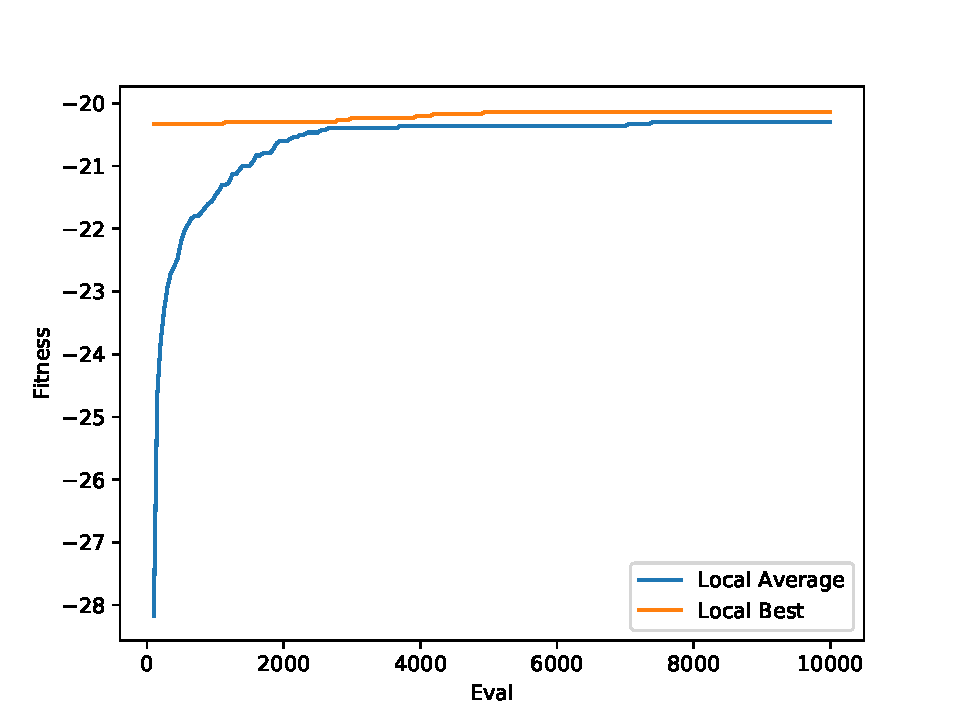
\includegraphics[width=\textwidth]{../graphs/graphs/1037.pdf}
\end{figure}


\begin{table}[!htb]
	\centering
	\caption{Figure \ref{fig:graph_1038} Configuration File}
	\label{tab:graph_1038}
	\begin{tabular}{| c | c |}
		\hline
		Search Algorithm		& EA		 \\
		\hline
		Termination Convergence Criterion		& 10000		 \\
		\hline
		Fitness Evaluations		& 10000		 \\
		\hline
		Survival Strategy		& Plus		 \\
		\hline
		Mutation Algorithm		& Flip		 \\
		\hline
		Placement Algorithm		& Random with Repair		 \\
		\hline
		Tournament Size For Parent Selection		& 5		 \\
		\hline
		Random Seed		& 1038		 \\
		\hline
		Self Adaptive Offspring Count		& True		 \\
		\hline
		Tournament Size For Survival Selection		& 5		 \\
		\hline
		Population Size		& 100		 \\
		\hline
		Survivor Algorithm		& Truncation		 \\
		\hline
		Offspring Count		& 50		 \\
		\hline
		Log File Path		& None		 \\
		\hline
		Penalty Coefficient		& 1		 \\
		\hline
		Parent Selection Algorithm		& k-Tournament Selection with replacement		 \\
		\hline
		Runs		& 30		 \\
		\hline
		Mutation Rate		& 0.1		 \\
		\hline
		Solution File Path		& None		 \\
		\hline
		Recombination Algorithm		& Partially Mapped Crossover		 \\
		\hline
		Self Adaptive Mutation Rate		& True		 \\
		\hline
		Self Adaptive Penalty Coefficient		& False		 \\
		\hline
	\end{tabular}
\end{table}
\begin{figure}[!htb]
	\caption{Input 1}
	\label{fig:graph_1038}
	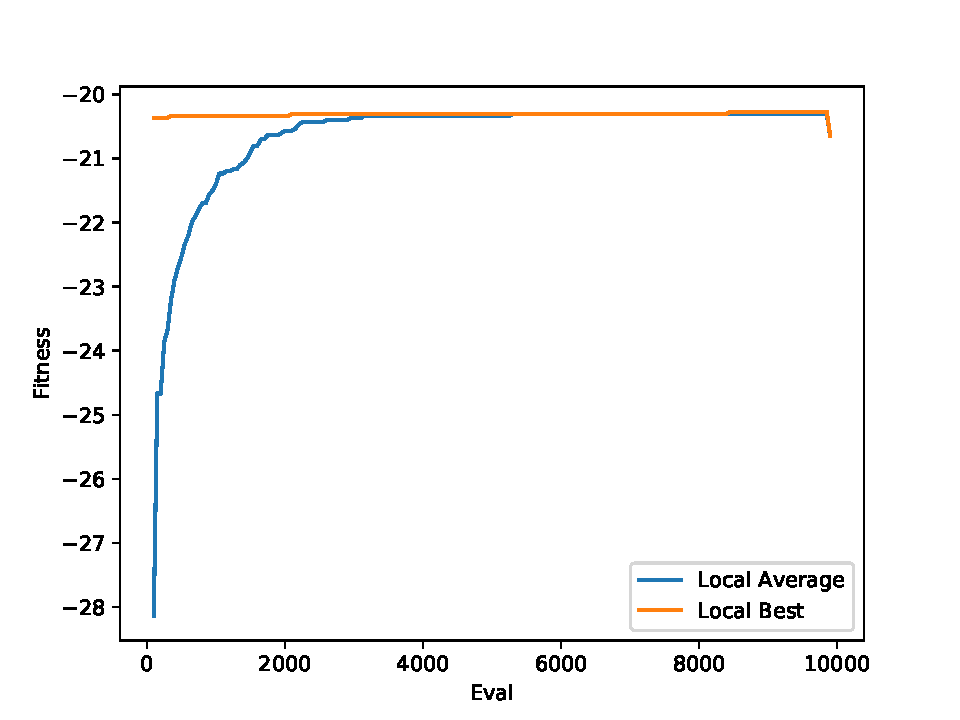
\includegraphics[width=\textwidth]{../graphs/graphs/1038.pdf}
\end{figure}


\begin{table}[!htb]
	\centering
	\caption{Figure \ref{fig:graph_1039} Configuration File}
	\label{tab:graph_1039}
	\begin{tabular}{| c | c |}
		\hline
		Search Algorithm		& EA		 \\
		\hline
		Termination Convergence Criterion		& 10000		 \\
		\hline
		Fitness Evaluations		& 10000		 \\
		\hline
		Survival Strategy		& Plus		 \\
		\hline
		Mutation Algorithm		& Flip		 \\
		\hline
		Placement Algorithm		& Random with Repair		 \\
		\hline
		Tournament Size For Parent Selection		& 5		 \\
		\hline
		Random Seed		& 1039		 \\
		\hline
		Self Adaptive Offspring Count		& False		 \\
		\hline
		Tournament Size For Survival Selection		& 5		 \\
		\hline
		Population Size		& 100		 \\
		\hline
		Survivor Algorithm		& Truncation		 \\
		\hline
		Offspring Count		& 50		 \\
		\hline
		Log File Path		& None		 \\
		\hline
		Penalty Coefficient		& 1		 \\
		\hline
		Parent Selection Algorithm		& k-Tournament Selection with replacement		 \\
		\hline
		Runs		& 30		 \\
		\hline
		Mutation Rate		& 0.1		 \\
		\hline
		Solution File Path		& None		 \\
		\hline
		Recombination Algorithm		& Partially Mapped Crossover		 \\
		\hline
		Self Adaptive Mutation Rate		& True		 \\
		\hline
		Self Adaptive Penalty Coefficient		& True		 \\
		\hline
	\end{tabular}
\end{table}
\begin{figure}[!htb]
	\caption{Input 1}
	\label{fig:graph_1039}
	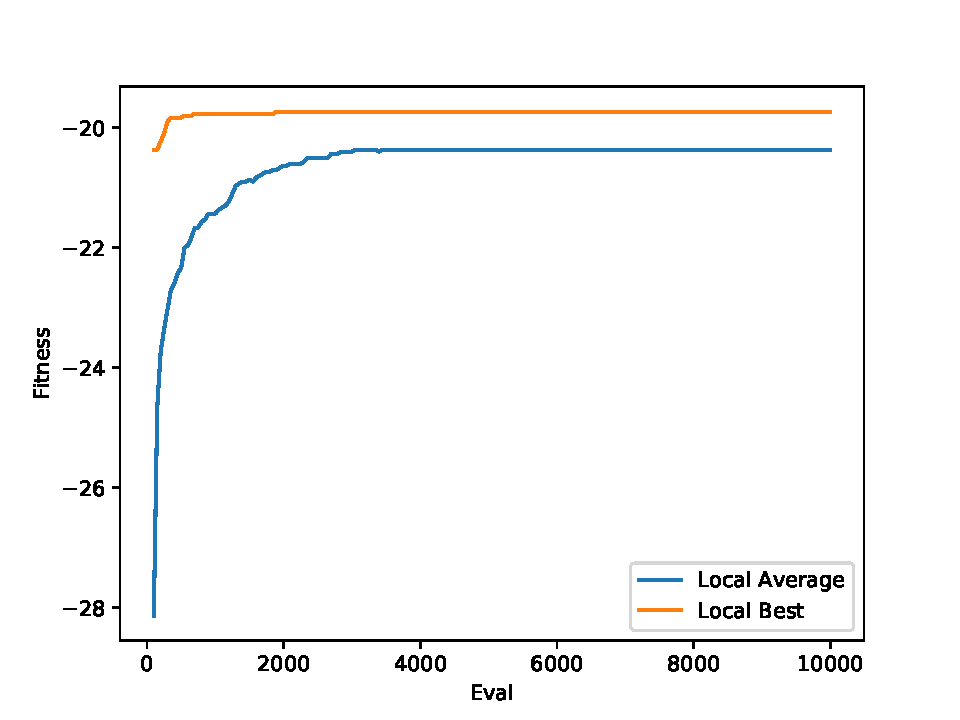
\includegraphics[width=\textwidth]{../graphs/graphs/1039.pdf}
\end{figure}


\begin{table}[!htb]
	\centering
	\caption{Figure \ref{fig:graph_1040} Configuration File}
	\label{tab:graph_1040}
	\begin{tabular}{| c | c |}
		\hline
		Search Algorithm		& EA		 \\
		\hline
		Termination Convergence Criterion		& 10000		 \\
		\hline
		Fitness Evaluations		& 10000		 \\
		\hline
		Survival Strategy		& Plus		 \\
		\hline
		Mutation Algorithm		& Flip		 \\
		\hline
		Placement Algorithm		& Random with Repair		 \\
		\hline
		Tournament Size For Parent Selection		& 5		 \\
		\hline
		Random Seed		& 1040		 \\
		\hline
		Self Adaptive Offspring Count		& True		 \\
		\hline
		Tournament Size For Survival Selection		& 5		 \\
		\hline
		Population Size		& 100		 \\
		\hline
		Survivor Algorithm		& Truncation		 \\
		\hline
		Offspring Count		& 50		 \\
		\hline
		Log File Path		& None		 \\
		\hline
		Penalty Coefficient		& 1		 \\
		\hline
		Parent Selection Algorithm		& k-Tournament Selection with replacement		 \\
		\hline
		Runs		& 30		 \\
		\hline
		Mutation Rate		& 0.1		 \\
		\hline
		Solution File Path		& None		 \\
		\hline
		Recombination Algorithm		& Partially Mapped Crossover		 \\
		\hline
		Self Adaptive Mutation Rate		& True		 \\
		\hline
		Self Adaptive Penalty Coefficient		& True		 \\
		\hline
	\end{tabular}
\end{table}
\begin{figure}[!htb]
	\caption{Input 1}
	\label{fig:graph_1040}
	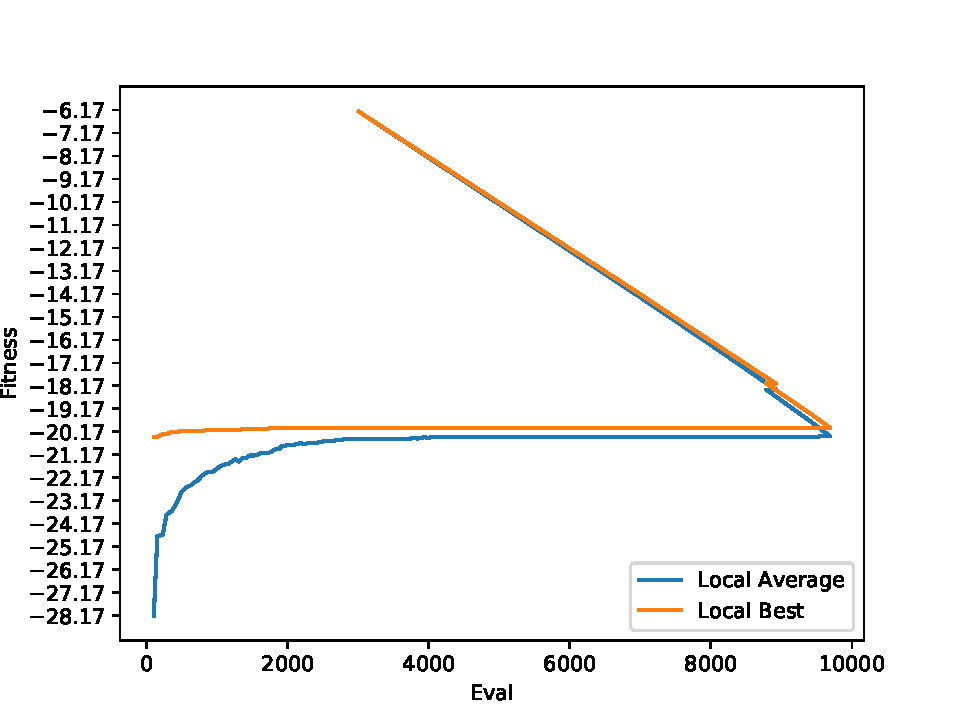
\includegraphics[width=\textwidth]{../graphs/graphs/1040.pdf}
\end{figure}


\clearpage
\begin{table}[!htb]
	\centering
	\caption{Figure \ref{fig:graph_1041} Configuration File}
	\label{tab:graph_1041}
	\begin{tabular}{| c | c |}
		\hline
		Search Algorithm		& EA		 \\
		\hline
		Termination Convergence Criterion		& 10000		 \\
		\hline
		Fitness Evaluations		& 10000		 \\
		\hline
		Survival Strategy		& Plus		 \\
		\hline
		Mutation Algorithm		& Flip		 \\
		\hline
		Placement Algorithm		& Random with Penalty		 \\
		\hline
		Tournament Size For Parent Selection		& 5		 \\
		\hline
		Random Seed		& 1041		 \\
		\hline
		Self Adaptive Offspring Count		& False		 \\
		\hline
		Tournament Size For Survival Selection		& 5		 \\
		\hline
		Population Size		& 100		 \\
		\hline
		Survivor Algorithm		& Truncation		 \\
		\hline
		Offspring Count		& 50		 \\
		\hline
		Log File Path		& None		 \\
		\hline
		Penalty Coefficient		& 1		 \\
		\hline
		Parent Selection Algorithm		& k-Tournament Selection with replacement		 \\
		\hline
		Runs		& 30		 \\
		\hline
		Mutation Rate		& 0.1		 \\
		\hline
		Solution File Path		& None		 \\
		\hline
		Recombination Algorithm		& Partially Mapped Crossover		 \\
		\hline
		Self Adaptive Mutation Rate		& False		 \\
		\hline
		Self Adaptive Penalty Coefficient		& False		 \\
		\hline
	\end{tabular}
\end{table}
\begin{figure}[!htb]
	\caption{Input 1}
	\label{fig:graph_1041}
	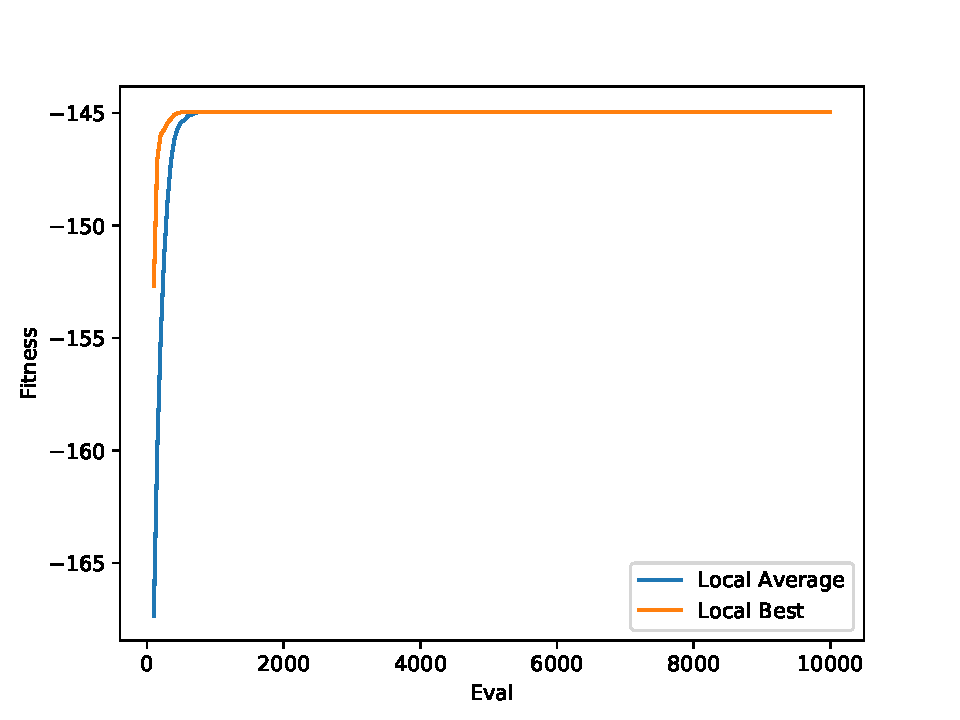
\includegraphics[width=\textwidth]{../graphs/graphs/1041.pdf}
\end{figure}


\begin{table}[!htb]
	\centering
	\caption{Figure \ref{fig:graph_1042} Configuration File}
	\label{tab:graph_1042}
	\begin{tabular}{| c | c |}
		\hline
		Search Algorithm		& EA		 \\
		\hline
		Termination Convergence Criterion		& 10000		 \\
		\hline
		Fitness Evaluations		& 10000		 \\
		\hline
		Survival Strategy		& Plus		 \\
		\hline
		Mutation Algorithm		& Flip		 \\
		\hline
		Placement Algorithm		& Random with Penalty		 \\
		\hline
		Tournament Size For Parent Selection		& 5		 \\
		\hline
		Random Seed		& 1042		 \\
		\hline
		Self Adaptive Offspring Count		& True		 \\
		\hline
		Tournament Size For Survival Selection		& 5		 \\
		\hline
		Population Size		& 100		 \\
		\hline
		Survivor Algorithm		& Truncation		 \\
		\hline
		Offspring Count		& 50		 \\
		\hline
		Log File Path		& None		 \\
		\hline
		Penalty Coefficient		& 1		 \\
		\hline
		Parent Selection Algorithm		& k-Tournament Selection with replacement		 \\
		\hline
		Runs		& 30		 \\
		\hline
		Mutation Rate		& 0.1		 \\
		\hline
		Solution File Path		& None		 \\
		\hline
		Recombination Algorithm		& Partially Mapped Crossover		 \\
		\hline
		Self Adaptive Mutation Rate		& False		 \\
		\hline
		Self Adaptive Penalty Coefficient		& False		 \\
		\hline
	\end{tabular}
\end{table}
\begin{figure}[!htb]
	\caption{Input 1}
	\label{fig:graph_1042}
	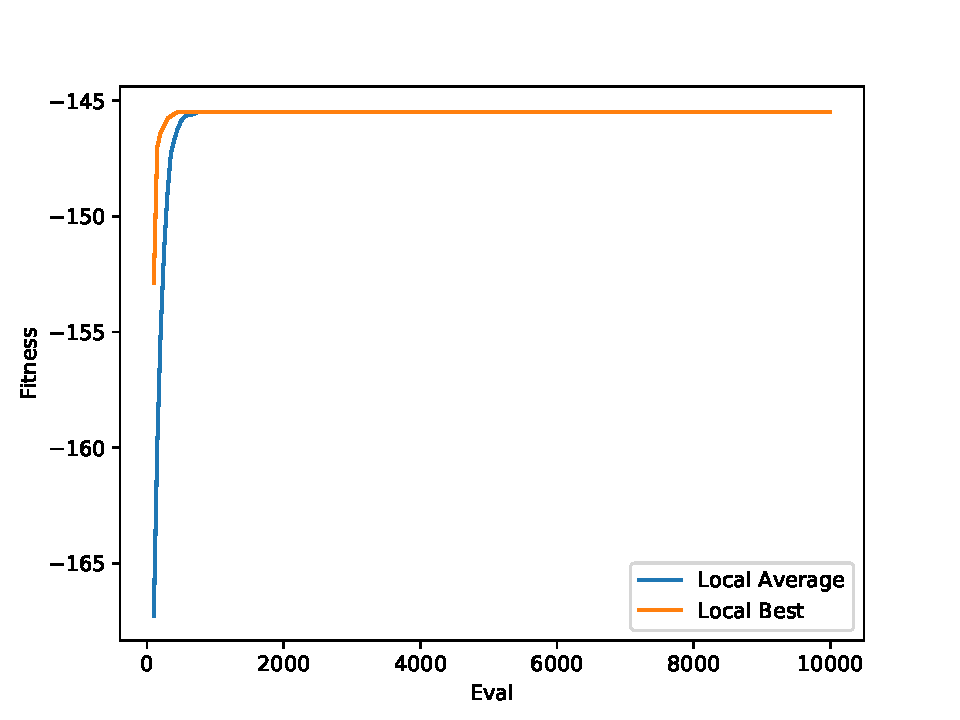
\includegraphics[width=\textwidth]{../graphs/graphs/1042.pdf}
\end{figure}


\begin{table}[!htb]
	\centering
	\caption{Figure \ref{fig:graph_1043} Configuration File}
	\label{tab:graph_1043}
	\begin{tabular}{| c | c |}
		\hline
		Search Algorithm		& EA		 \\
		\hline
		Termination Convergence Criterion		& 10000		 \\
		\hline
		Fitness Evaluations		& 10000		 \\
		\hline
		Survival Strategy		& Plus		 \\
		\hline
		Mutation Algorithm		& Flip		 \\
		\hline
		Placement Algorithm		& Random with Penalty		 \\
		\hline
		Tournament Size For Parent Selection		& 5		 \\
		\hline
		Random Seed		& 1043		 \\
		\hline
		Self Adaptive Offspring Count		& False		 \\
		\hline
		Tournament Size For Survival Selection		& 5		 \\
		\hline
		Population Size		& 100		 \\
		\hline
		Survivor Algorithm		& Truncation		 \\
		\hline
		Offspring Count		& 50		 \\
		\hline
		Log File Path		& None		 \\
		\hline
		Penalty Coefficient		& 1		 \\
		\hline
		Parent Selection Algorithm		& k-Tournament Selection with replacement		 \\
		\hline
		Runs		& 30		 \\
		\hline
		Mutation Rate		& 0.1		 \\
		\hline
		Solution File Path		& None		 \\
		\hline
		Recombination Algorithm		& Partially Mapped Crossover		 \\
		\hline
		Self Adaptive Mutation Rate		& False		 \\
		\hline
		Self Adaptive Penalty Coefficient		& True		 \\
		\hline
	\end{tabular}
\end{table}
\begin{figure}[!htb]
	\caption{Input 1}
	\label{fig:graph_1043}
	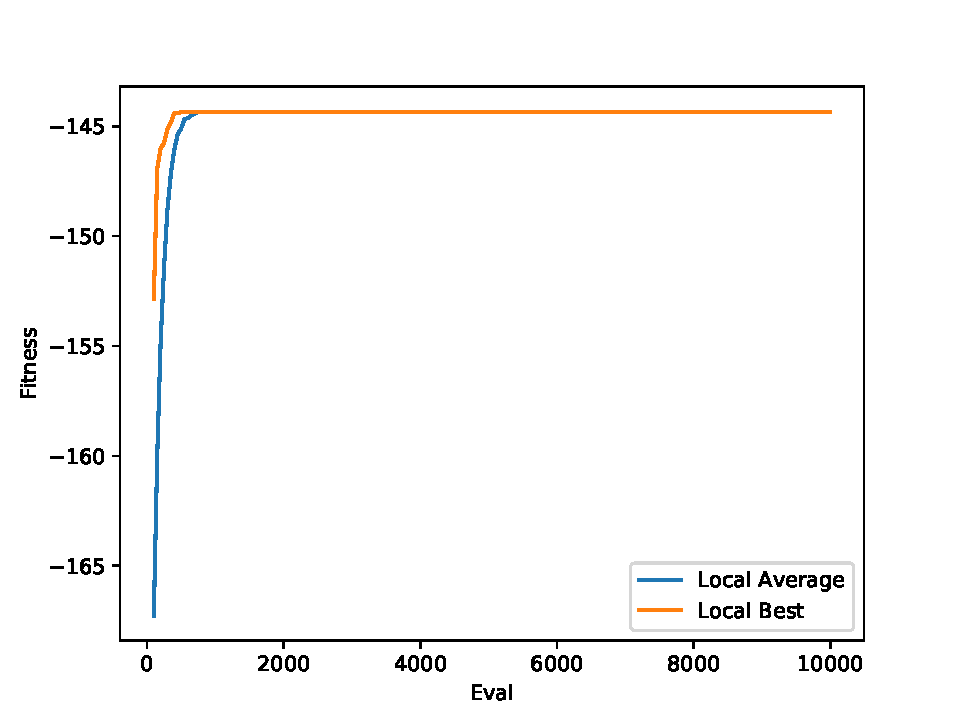
\includegraphics[width=\textwidth]{../graphs/graphs/1043.pdf}
\end{figure}


\begin{table}[!htb]
	\centering
	\caption{Figure \ref{fig:graph_1044} Configuration File}
	\label{tab:graph_1044}
	\begin{tabular}{| c | c |}
		\hline
		Search Algorithm		& EA		 \\
		\hline
		Termination Convergence Criterion		& 10000		 \\
		\hline
		Fitness Evaluations		& 10000		 \\
		\hline
		Survival Strategy		& Plus		 \\
		\hline
		Mutation Algorithm		& Flip		 \\
		\hline
		Placement Algorithm		& Random with Penalty		 \\
		\hline
		Tournament Size For Parent Selection		& 5		 \\
		\hline
		Random Seed		& 1044		 \\
		\hline
		Self Adaptive Offspring Count		& True		 \\
		\hline
		Tournament Size For Survival Selection		& 5		 \\
		\hline
		Population Size		& 100		 \\
		\hline
		Survivor Algorithm		& Truncation		 \\
		\hline
		Offspring Count		& 50		 \\
		\hline
		Log File Path		& None		 \\
		\hline
		Penalty Coefficient		& 1		 \\
		\hline
		Parent Selection Algorithm		& k-Tournament Selection with replacement		 \\
		\hline
		Runs		& 30		 \\
		\hline
		Mutation Rate		& 0.1		 \\
		\hline
		Solution File Path		& None		 \\
		\hline
		Recombination Algorithm		& Partially Mapped Crossover		 \\
		\hline
		Self Adaptive Mutation Rate		& False		 \\
		\hline
		Self Adaptive Penalty Coefficient		& True		 \\
		\hline
	\end{tabular}
\end{table}
\begin{figure}[!htb]
	\caption{Input 1}
	\label{fig:graph_1044}
	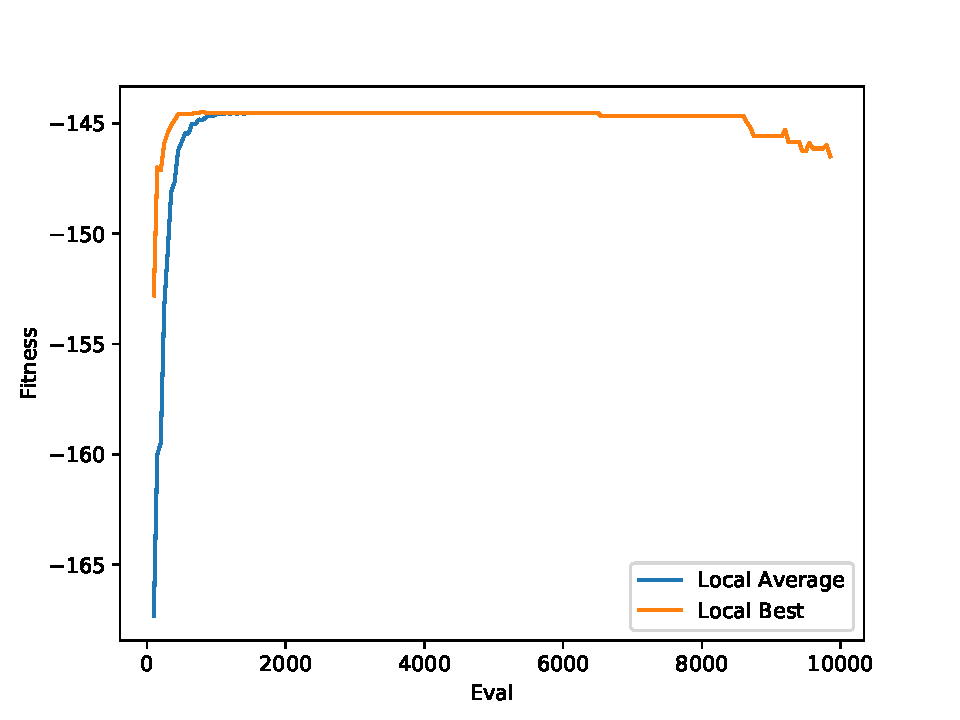
\includegraphics[width=\textwidth]{../graphs/graphs/1044.pdf}
\end{figure}


\begin{table}[!htb]
	\centering
	\caption{Figure \ref{fig:graph_1045} Configuration File}
	\label{tab:graph_1045}
	\begin{tabular}{| c | c |}
		\hline
		Search Algorithm		& EA		 \\
		\hline
		Termination Convergence Criterion		& 10000		 \\
		\hline
		Fitness Evaluations		& 10000		 \\
		\hline
		Survival Strategy		& Plus		 \\
		\hline
		Mutation Algorithm		& Flip		 \\
		\hline
		Placement Algorithm		& Random with Penalty		 \\
		\hline
		Tournament Size For Parent Selection		& 5		 \\
		\hline
		Random Seed		& 1045		 \\
		\hline
		Self Adaptive Offspring Count		& False		 \\
		\hline
		Tournament Size For Survival Selection		& 5		 \\
		\hline
		Population Size		& 100		 \\
		\hline
		Survivor Algorithm		& Truncation		 \\
		\hline
		Offspring Count		& 50		 \\
		\hline
		Log File Path		& None		 \\
		\hline
		Penalty Coefficient		& 1		 \\
		\hline
		Parent Selection Algorithm		& k-Tournament Selection with replacement		 \\
		\hline
		Runs		& 30		 \\
		\hline
		Mutation Rate		& 0.1		 \\
		\hline
		Solution File Path		& None		 \\
		\hline
		Recombination Algorithm		& Partially Mapped Crossover		 \\
		\hline
		Self Adaptive Mutation Rate		& True		 \\
		\hline
		Self Adaptive Penalty Coefficient		& False		 \\
		\hline
	\end{tabular}
\end{table}
\begin{figure}[!htb]
	\caption{Input 1}
	\label{fig:graph_1045}
	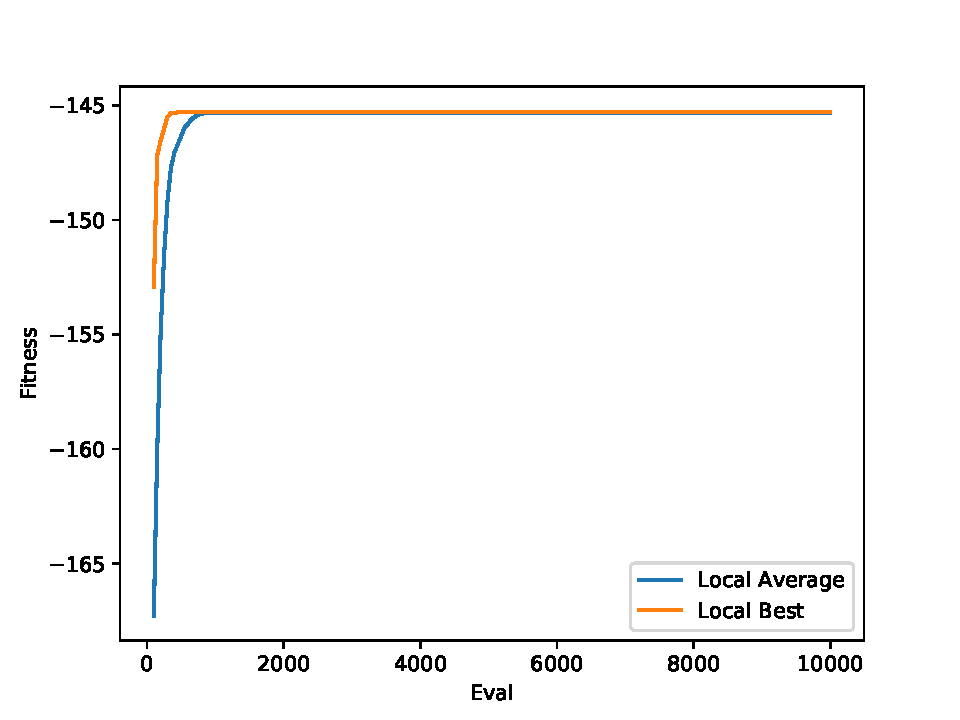
\includegraphics[width=\textwidth]{../graphs/graphs/1045.pdf}
\end{figure}


\begin{table}[!htb]
	\centering
	\caption{Figure \ref{fig:graph_1046} Configuration File}
	\label{tab:graph_1046}
	\begin{tabular}{| c | c |}
		\hline
		Search Algorithm		& EA		 \\
		\hline
		Termination Convergence Criterion		& 10000		 \\
		\hline
		Fitness Evaluations		& 10000		 \\
		\hline
		Survival Strategy		& Plus		 \\
		\hline
		Mutation Algorithm		& Flip		 \\
		\hline
		Placement Algorithm		& Random with Penalty		 \\
		\hline
		Tournament Size For Parent Selection		& 5		 \\
		\hline
		Random Seed		& 1046		 \\
		\hline
		Self Adaptive Offspring Count		& True		 \\
		\hline
		Tournament Size For Survival Selection		& 5		 \\
		\hline
		Population Size		& 100		 \\
		\hline
		Survivor Algorithm		& Truncation		 \\
		\hline
		Offspring Count		& 50		 \\
		\hline
		Log File Path		& None		 \\
		\hline
		Penalty Coefficient		& 1		 \\
		\hline
		Parent Selection Algorithm		& k-Tournament Selection with replacement		 \\
		\hline
		Runs		& 30		 \\
		\hline
		Mutation Rate		& 0.1		 \\
		\hline
		Solution File Path		& None		 \\
		\hline
		Recombination Algorithm		& Partially Mapped Crossover		 \\
		\hline
		Self Adaptive Mutation Rate		& True		 \\
		\hline
		Self Adaptive Penalty Coefficient		& False		 \\
		\hline
	\end{tabular}
\end{table}
\begin{figure}[!htb]
	\caption{Input 1}
	\label{fig:graph_1046}
	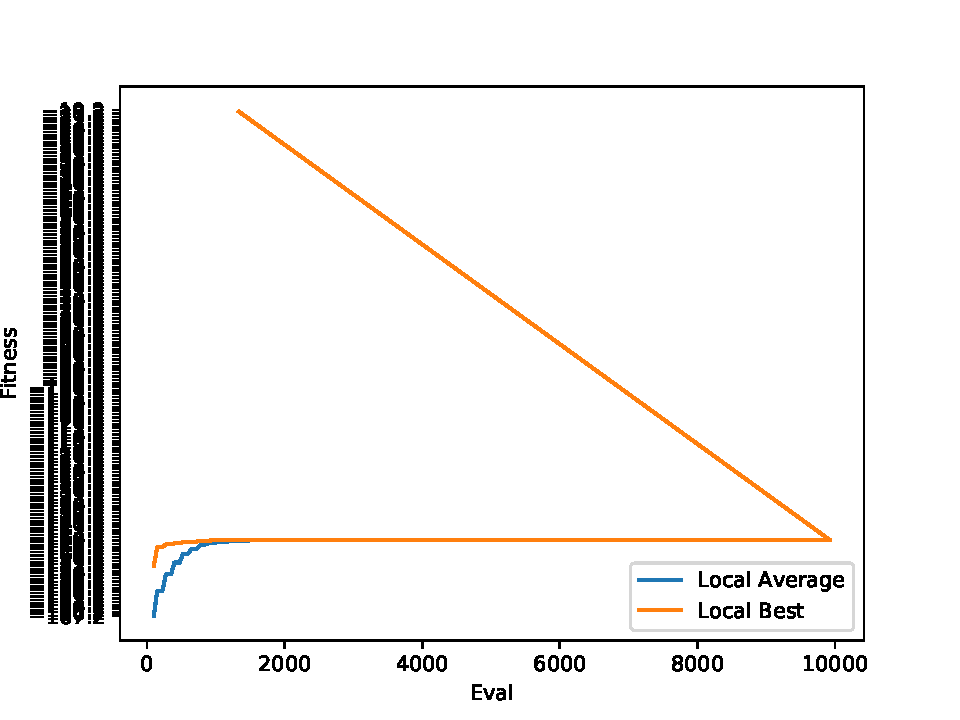
\includegraphics[width=\textwidth]{../graphs/graphs/1046.pdf}
\end{figure}


\begin{table}[!htb]
	\centering
	\caption{Figure \ref{fig:graph_1047} Configuration File}
	\label{tab:graph_1047}
	\begin{tabular}{| c | c |}
		\hline
		Search Algorithm		& EA		 \\
		\hline
		Termination Convergence Criterion		& 10000		 \\
		\hline
		Fitness Evaluations		& 10000		 \\
		\hline
		Survival Strategy		& Plus		 \\
		\hline
		Mutation Algorithm		& Flip		 \\
		\hline
		Placement Algorithm		& Random with Penalty		 \\
		\hline
		Tournament Size For Parent Selection		& 5		 \\
		\hline
		Random Seed		& 1047		 \\
		\hline
		Self Adaptive Offspring Count		& False		 \\
		\hline
		Tournament Size For Survival Selection		& 5		 \\
		\hline
		Population Size		& 100		 \\
		\hline
		Survivor Algorithm		& Truncation		 \\
		\hline
		Offspring Count		& 50		 \\
		\hline
		Log File Path		& None		 \\
		\hline
		Penalty Coefficient		& 1		 \\
		\hline
		Parent Selection Algorithm		& k-Tournament Selection with replacement		 \\
		\hline
		Runs		& 30		 \\
		\hline
		Mutation Rate		& 0.1		 \\
		\hline
		Solution File Path		& None		 \\
		\hline
		Recombination Algorithm		& Partially Mapped Crossover		 \\
		\hline
		Self Adaptive Mutation Rate		& True		 \\
		\hline
		Self Adaptive Penalty Coefficient		& True		 \\
		\hline
	\end{tabular}
\end{table}
\begin{figure}[!htb]
	\caption{Input 1}
	\label{fig:graph_1047}
	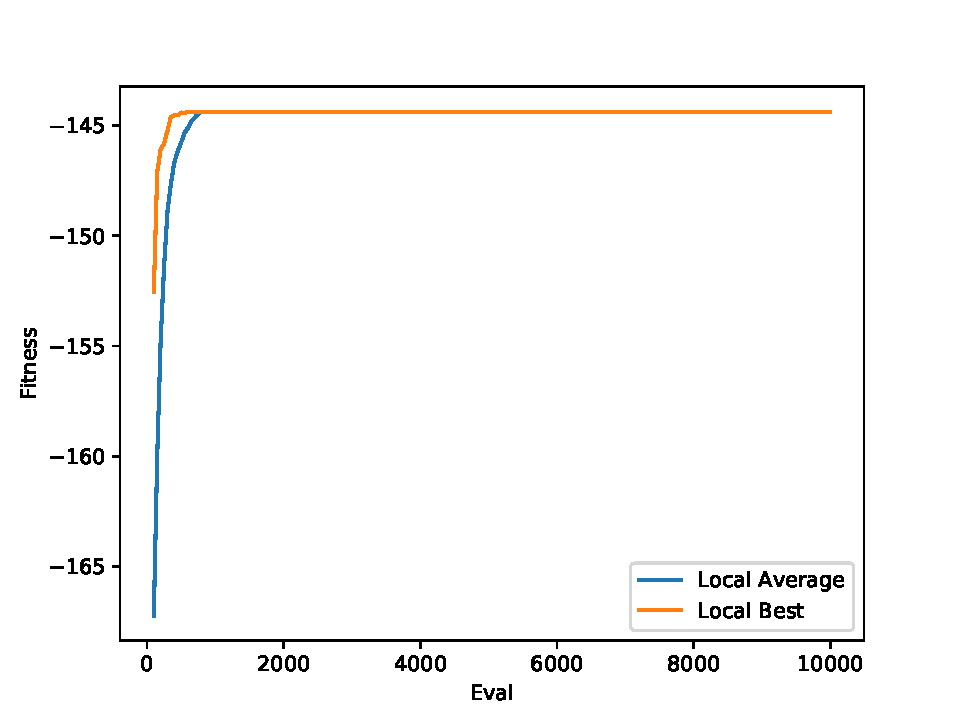
\includegraphics[width=\textwidth]{../graphs/graphs/1047.pdf}
\end{figure}


\begin{table}[!htb]
	\centering
	\caption{Figure \ref{fig:graph_1048} Configuration File}
	\label{tab:graph_1048}
	\begin{tabular}{| c | c |}
		\hline
		Search Algorithm		& EA		 \\
		\hline
		Termination Convergence Criterion		& 10000		 \\
		\hline
		Fitness Evaluations		& 10000		 \\
		\hline
		Survival Strategy		& Plus		 \\
		\hline
		Mutation Algorithm		& Flip		 \\
		\hline
		Placement Algorithm		& Random with Penalty		 \\
		\hline
		Tournament Size For Parent Selection		& 5		 \\
		\hline
		Random Seed		& 1048		 \\
		\hline
		Self Adaptive Offspring Count		& True		 \\
		\hline
		Tournament Size For Survival Selection		& 5		 \\
		\hline
		Population Size		& 100		 \\
		\hline
		Survivor Algorithm		& Truncation		 \\
		\hline
		Offspring Count		& 50		 \\
		\hline
		Log File Path		& None		 \\
		\hline
		Penalty Coefficient		& 1		 \\
		\hline
		Parent Selection Algorithm		& k-Tournament Selection with replacement		 \\
		\hline
		Runs		& 30		 \\
		\hline
		Mutation Rate		& 0.1		 \\
		\hline
		Solution File Path		& None		 \\
		\hline
		Recombination Algorithm		& Partially Mapped Crossover		 \\
		\hline
		Self Adaptive Mutation Rate		& True		 \\
		\hline
		Self Adaptive Penalty Coefficient		& True		 \\
		\hline
	\end{tabular}
\end{table}
\begin{figure}[!htb]
	\caption{Input 1}
	\label{fig:graph_1048}
	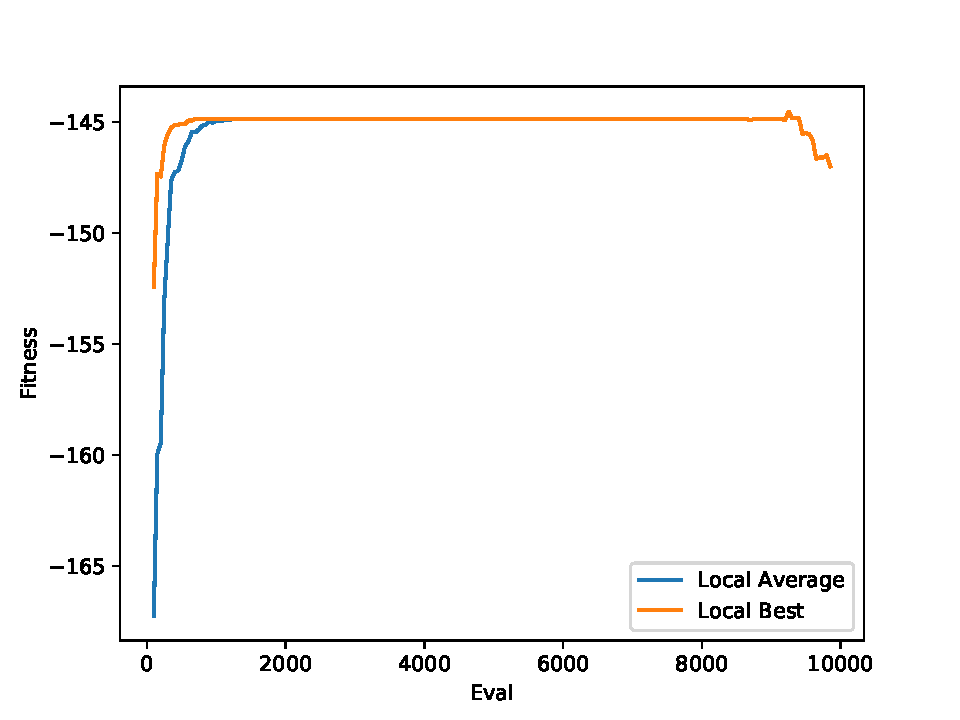
\includegraphics[width=\textwidth]{../graphs/graphs/1048.pdf}
\end{figure}


\begin{table}[!htb]
	\centering
	\caption{Figure \ref{fig:graph_1049} Configuration File}
	\label{tab:graph_1049}
	\begin{tabular}{| c | c |}
		\hline
		Search Algorithm		& EA		 \\
		\hline
		Termination Convergence Criterion		& 10000		 \\
		\hline
		Fitness Evaluations		& 10000		 \\
		\hline
		Survival Strategy		& Plus		 \\
		\hline
		Mutation Algorithm		& Flip		 \\
		\hline
		Placement Algorithm		& Random		 \\
		\hline
		Tournament Size For Parent Selection		& 5		 \\
		\hline
		Random Seed		& 1049		 \\
		\hline
		Self Adaptive Offspring Count		& False		 \\
		\hline
		Tournament Size For Survival Selection		& 5		 \\
		\hline
		Population Size		& 100		 \\
		\hline
		Survivor Algorithm		& Truncation		 \\
		\hline
		Offspring Count		& 50		 \\
		\hline
		Log File Path		& None		 \\
		\hline
		Penalty Coefficient		& 1		 \\
		\hline
		Parent Selection Algorithm		& k-Tournament Selection with replacement		 \\
		\hline
		Runs		& 30		 \\
		\hline
		Mutation Rate		& 0.1		 \\
		\hline
		Solution File Path		& None		 \\
		\hline
		Recombination Algorithm		& Order Crossover		 \\
		\hline
		Self Adaptive Mutation Rate		& False		 \\
		\hline
		Self Adaptive Penalty Coefficient		& False		 \\
		\hline
	\end{tabular}
\end{table}
\begin{figure}[!htb]
	\caption{Input 1}
	\label{fig:graph_1049}
	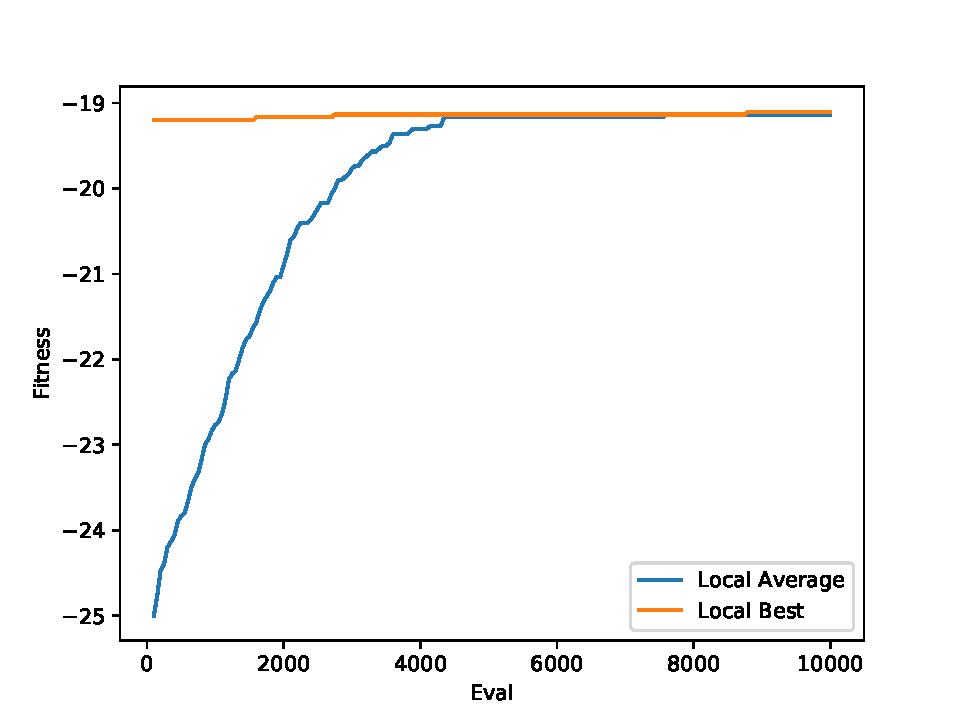
\includegraphics[width=\textwidth]{../graphs/graphs/1049.pdf}
\end{figure}


\begin{table}[!htb]
	\centering
	\caption{Figure \ref{fig:graph_1050} Configuration File}
	\label{tab:graph_1050}
	\begin{tabular}{| c | c |}
		\hline
		Search Algorithm		& EA		 \\
		\hline
		Termination Convergence Criterion		& 10000		 \\
		\hline
		Fitness Evaluations		& 10000		 \\
		\hline
		Survival Strategy		& Plus		 \\
		\hline
		Mutation Algorithm		& Move		 \\
		\hline
		Placement Algorithm		& Random		 \\
		\hline
		Tournament Size For Parent Selection		& 5		 \\
		\hline
		Random Seed		& 1050		 \\
		\hline
		Self Adaptive Offspring Count		& False		 \\
		\hline
		Tournament Size For Survival Selection		& 5		 \\
		\hline
		Population Size		& 100		 \\
		\hline
		Survivor Algorithm		& Truncation		 \\
		\hline
		Offspring Count		& 50		 \\
		\hline
		Log File Path		& None		 \\
		\hline
		Penalty Coefficient		& 1		 \\
		\hline
		Parent Selection Algorithm		& k-Tournament Selection with replacement		 \\
		\hline
		Runs		& 30		 \\
		\hline
		Mutation Rate		& 0.1		 \\
		\hline
		Solution File Path		& None		 \\
		\hline
		Recombination Algorithm		& Order Crossover		 \\
		\hline
		Self Adaptive Mutation Rate		& False		 \\
		\hline
		Self Adaptive Penalty Coefficient		& False		 \\
		\hline
	\end{tabular}
\end{table}
\begin{figure}[!htb]
	\caption{Input 1}
	\label{fig:graph_1050}
	\includegraphics[width=\textwidth]{../graphs/graphs/1050.pdf}
\end{figure}


\clearpage
\begin{table}[!htb]
	\centering
	\caption{Figure \ref{fig:graph_1051} Configuration File}
	\label{tab:graph_1051}
	\begin{tabular}{| c | c |}
		\hline
		Search Algorithm		& EA		 \\
		\hline
		Termination Convergence Criterion		& 10000		 \\
		\hline
		Fitness Evaluations		& 10000		 \\
		\hline
		Survival Strategy		& Plus		 \\
		\hline
		Mutation Algorithm		& Flip		 \\
		\hline
		Placement Algorithm		& Random		 \\
		\hline
		Tournament Size For Parent Selection		& 5		 \\
		\hline
		Random Seed		& 1051		 \\
		\hline
		Self Adaptive Offspring Count		& True		 \\
		\hline
		Tournament Size For Survival Selection		& 5		 \\
		\hline
		Population Size		& 100		 \\
		\hline
		Survivor Algorithm		& Truncation		 \\
		\hline
		Offspring Count		& 50		 \\
		\hline
		Log File Path		& None		 \\
		\hline
		Penalty Coefficient		& 1		 \\
		\hline
		Parent Selection Algorithm		& k-Tournament Selection with replacement		 \\
		\hline
		Runs		& 30		 \\
		\hline
		Mutation Rate		& 0.1		 \\
		\hline
		Solution File Path		& None		 \\
		\hline
		Recombination Algorithm		& Order Crossover		 \\
		\hline
		Self Adaptive Mutation Rate		& False		 \\
		\hline
		Self Adaptive Penalty Coefficient		& False		 \\
		\hline
	\end{tabular}
\end{table}
\begin{figure}[!htb]
	\caption{Input 1}
	\label{fig:graph_1051}
	\includegraphics[width=\textwidth]{../graphs/graphs/1051.pdf}
\end{figure}


\begin{table}[!htb]
	\centering
	\caption{Figure \ref{fig:graph_1052} Configuration File}
	\label{tab:graph_1052}
	\begin{tabular}{| c | c |}
		\hline
		Search Algorithm		& EA		 \\
		\hline
		Termination Convergence Criterion		& 10000		 \\
		\hline
		Fitness Evaluations		& 10000		 \\
		\hline
		Survival Strategy		& Plus		 \\
		\hline
		Mutation Algorithm		& Move		 \\
		\hline
		Placement Algorithm		& Random		 \\
		\hline
		Tournament Size For Parent Selection		& 5		 \\
		\hline
		Random Seed		& 1052		 \\
		\hline
		Self Adaptive Offspring Count		& True		 \\
		\hline
		Tournament Size For Survival Selection		& 5		 \\
		\hline
		Population Size		& 100		 \\
		\hline
		Survivor Algorithm		& Truncation		 \\
		\hline
		Offspring Count		& 50		 \\
		\hline
		Log File Path		& None		 \\
		\hline
		Penalty Coefficient		& 1		 \\
		\hline
		Parent Selection Algorithm		& k-Tournament Selection with replacement		 \\
		\hline
		Runs		& 30		 \\
		\hline
		Mutation Rate		& 0.1		 \\
		\hline
		Solution File Path		& None		 \\
		\hline
		Recombination Algorithm		& Order Crossover		 \\
		\hline
		Self Adaptive Mutation Rate		& False		 \\
		\hline
		Self Adaptive Penalty Coefficient		& False		 \\
		\hline
	\end{tabular}
\end{table}
\begin{figure}[!htb]
	\caption{Input 1}
	\label{fig:graph_1052}
	\includegraphics[width=\textwidth]{../graphs/graphs/1052.pdf}
\end{figure}


\begin{table}[!htb]
	\centering
	\caption{Figure \ref{fig:graph_1053} Configuration File}
	\label{tab:graph_1053}
	\begin{tabular}{| c | c |}
		\hline
		Search Algorithm		& EA		 \\
		\hline
		Termination Convergence Criterion		& 10000		 \\
		\hline
		Fitness Evaluations		& 10000		 \\
		\hline
		Survival Strategy		& Plus		 \\
		\hline
		Mutation Algorithm		& Flip		 \\
		\hline
		Placement Algorithm		& Random		 \\
		\hline
		Tournament Size For Parent Selection		& 5		 \\
		\hline
		Random Seed		& 1053		 \\
		\hline
		Self Adaptive Offspring Count		& False		 \\
		\hline
		Tournament Size For Survival Selection		& 5		 \\
		\hline
		Population Size		& 100		 \\
		\hline
		Survivor Algorithm		& Truncation		 \\
		\hline
		Offspring Count		& 50		 \\
		\hline
		Log File Path		& None		 \\
		\hline
		Penalty Coefficient		& 1		 \\
		\hline
		Parent Selection Algorithm		& k-Tournament Selection with replacement		 \\
		\hline
		Runs		& 30		 \\
		\hline
		Mutation Rate		& 0.1		 \\
		\hline
		Solution File Path		& None		 \\
		\hline
		Recombination Algorithm		& Order Crossover		 \\
		\hline
		Self Adaptive Mutation Rate		& True		 \\
		\hline
		Self Adaptive Penalty Coefficient		& False		 \\
		\hline
	\end{tabular}
\end{table}
\begin{figure}[!htb]
	\caption{Input 1}
	\label{fig:graph_1053}
	\includegraphics[width=\textwidth]{../graphs/graphs/1053.pdf}
\end{figure}


\begin{table}[!htb]
	\centering
	\caption{Figure \ref{fig:graph_1054} Configuration File}
	\label{tab:graph_1054}
	\begin{tabular}{| c | c |}
		\hline
		Search Algorithm		& EA		 \\
		\hline
		Termination Convergence Criterion		& 10000		 \\
		\hline
		Fitness Evaluations		& 10000		 \\
		\hline
		Survival Strategy		& Plus		 \\
		\hline
		Mutation Algorithm		& Move		 \\
		\hline
		Placement Algorithm		& Random		 \\
		\hline
		Tournament Size For Parent Selection		& 5		 \\
		\hline
		Random Seed		& 1054		 \\
		\hline
		Self Adaptive Offspring Count		& False		 \\
		\hline
		Tournament Size For Survival Selection		& 5		 \\
		\hline
		Population Size		& 100		 \\
		\hline
		Survivor Algorithm		& Truncation		 \\
		\hline
		Offspring Count		& 50		 \\
		\hline
		Log File Path		& None		 \\
		\hline
		Penalty Coefficient		& 1		 \\
		\hline
		Parent Selection Algorithm		& k-Tournament Selection with replacement		 \\
		\hline
		Runs		& 30		 \\
		\hline
		Mutation Rate		& 0.1		 \\
		\hline
		Solution File Path		& None		 \\
		\hline
		Recombination Algorithm		& Order Crossover		 \\
		\hline
		Self Adaptive Mutation Rate		& True		 \\
		\hline
		Self Adaptive Penalty Coefficient		& False		 \\
		\hline
	\end{tabular}
\end{table}
\begin{figure}[!htb]
	\caption{Input 1}
	\label{fig:graph_1054}
	\includegraphics[width=\textwidth]{../graphs/graphs/1054.pdf}
\end{figure}


\begin{table}[!htb]
	\centering
	\caption{Figure \ref{fig:graph_1055} Configuration File}
	\label{tab:graph_1055}
	\begin{tabular}{| c | c |}
		\hline
		Search Algorithm		& EA		 \\
		\hline
		Termination Convergence Criterion		& 10000		 \\
		\hline
		Fitness Evaluations		& 10000		 \\
		\hline
		Survival Strategy		& Plus		 \\
		\hline
		Mutation Algorithm		& Flip		 \\
		\hline
		Placement Algorithm		& Random		 \\
		\hline
		Tournament Size For Parent Selection		& 5		 \\
		\hline
		Random Seed		& 1055		 \\
		\hline
		Self Adaptive Offspring Count		& True		 \\
		\hline
		Tournament Size For Survival Selection		& 5		 \\
		\hline
		Population Size		& 100		 \\
		\hline
		Survivor Algorithm		& Truncation		 \\
		\hline
		Offspring Count		& 50		 \\
		\hline
		Log File Path		& None		 \\
		\hline
		Penalty Coefficient		& 1		 \\
		\hline
		Parent Selection Algorithm		& k-Tournament Selection with replacement		 \\
		\hline
		Runs		& 30		 \\
		\hline
		Mutation Rate		& 0.1		 \\
		\hline
		Solution File Path		& None		 \\
		\hline
		Recombination Algorithm		& Order Crossover		 \\
		\hline
		Self Adaptive Mutation Rate		& True		 \\
		\hline
		Self Adaptive Penalty Coefficient		& False		 \\
		\hline
	\end{tabular}
\end{table}
\begin{figure}[!htb]
	\caption{Input 1}
	\label{fig:graph_1055}
	\includegraphics[width=\textwidth]{../graphs/graphs/1055.pdf}
\end{figure}


\begin{table}[!htb]
	\centering
	\caption{Figure \ref{fig:graph_1056} Configuration File}
	\label{tab:graph_1056}
	\begin{tabular}{| c | c |}
		\hline
		Search Algorithm		& EA		 \\
		\hline
		Termination Convergence Criterion		& 10000		 \\
		\hline
		Fitness Evaluations		& 10000		 \\
		\hline
		Survival Strategy		& Plus		 \\
		\hline
		Mutation Algorithm		& Move		 \\
		\hline
		Placement Algorithm		& Random		 \\
		\hline
		Tournament Size For Parent Selection		& 5		 \\
		\hline
		Random Seed		& 1056		 \\
		\hline
		Self Adaptive Offspring Count		& True		 \\
		\hline
		Tournament Size For Survival Selection		& 5		 \\
		\hline
		Population Size		& 100		 \\
		\hline
		Survivor Algorithm		& Truncation		 \\
		\hline
		Offspring Count		& 50		 \\
		\hline
		Log File Path		& None		 \\
		\hline
		Penalty Coefficient		& 1		 \\
		\hline
		Parent Selection Algorithm		& k-Tournament Selection with replacement		 \\
		\hline
		Runs		& 30		 \\
		\hline
		Mutation Rate		& 0.1		 \\
		\hline
		Solution File Path		& None		 \\
		\hline
		Recombination Algorithm		& Order Crossover		 \\
		\hline
		Self Adaptive Mutation Rate		& True		 \\
		\hline
		Self Adaptive Penalty Coefficient		& False		 \\
		\hline
	\end{tabular}
\end{table}
\begin{figure}[!htb]
	\caption{Input 1}
	\label{fig:graph_1056}
	\includegraphics[width=\textwidth]{../graphs/graphs/1056.pdf}
\end{figure}


\begin{table}[!htb]
	\centering
	\caption{Figure \ref{fig:graph_1057} Configuration File}
	\label{tab:graph_1057}
	\begin{tabular}{| c | c |}
		\hline
		Search Algorithm		& EA		 \\
		\hline
		Termination Convergence Criterion		& 10000		 \\
		\hline
		Fitness Evaluations		& 10000		 \\
		\hline
		Survival Strategy		& Plus		 \\
		\hline
		Mutation Algorithm		& Flip		 \\
		\hline
		Placement Algorithm		& Random with Repair		 \\
		\hline
		Tournament Size For Parent Selection		& 5		 \\
		\hline
		Random Seed		& 1057		 \\
		\hline
		Self Adaptive Offspring Count		& False		 \\
		\hline
		Tournament Size For Survival Selection		& 5		 \\
		\hline
		Population Size		& 100		 \\
		\hline
		Survivor Algorithm		& Truncation		 \\
		\hline
		Offspring Count		& 50		 \\
		\hline
		Log File Path		& None		 \\
		\hline
		Penalty Coefficient		& 1		 \\
		\hline
		Parent Selection Algorithm		& k-Tournament Selection with replacement		 \\
		\hline
		Runs		& 30		 \\
		\hline
		Mutation Rate		& 0.1		 \\
		\hline
		Solution File Path		& None		 \\
		\hline
		Recombination Algorithm		& Order Crossover		 \\
		\hline
		Self Adaptive Mutation Rate		& False		 \\
		\hline
		Self Adaptive Penalty Coefficient		& False		 \\
		\hline
	\end{tabular}
\end{table}
\begin{figure}[!htb]
	\caption{Input 1}
	\label{fig:graph_1057}
	\includegraphics[width=\textwidth]{../graphs/graphs/1057.pdf}
\end{figure}


\begin{table}[!htb]
	\centering
	\caption{Figure \ref{fig:graph_1058} Configuration File}
	\label{tab:graph_1058}
	\begin{tabular}{| c | c |}
		\hline
		Search Algorithm		& EA		 \\
		\hline
		Termination Convergence Criterion		& 10000		 \\
		\hline
		Fitness Evaluations		& 10000		 \\
		\hline
		Survival Strategy		& Plus		 \\
		\hline
		Mutation Algorithm		& Move		 \\
		\hline
		Placement Algorithm		& Random with Repair		 \\
		\hline
		Tournament Size For Parent Selection		& 5		 \\
		\hline
		Random Seed		& 1058		 \\
		\hline
		Self Adaptive Offspring Count		& False		 \\
		\hline
		Tournament Size For Survival Selection		& 5		 \\
		\hline
		Population Size		& 100		 \\
		\hline
		Survivor Algorithm		& Truncation		 \\
		\hline
		Offspring Count		& 50		 \\
		\hline
		Log File Path		& None		 \\
		\hline
		Penalty Coefficient		& 1		 \\
		\hline
		Parent Selection Algorithm		& k-Tournament Selection with replacement		 \\
		\hline
		Runs		& 30		 \\
		\hline
		Mutation Rate		& 0.1		 \\
		\hline
		Solution File Path		& None		 \\
		\hline
		Recombination Algorithm		& Order Crossover		 \\
		\hline
		Self Adaptive Mutation Rate		& False		 \\
		\hline
		Self Adaptive Penalty Coefficient		& False		 \\
		\hline
	\end{tabular}
\end{table}
\begin{figure}[!htb]
	\caption{Input 1}
	\label{fig:graph_1058}
	\includegraphics[width=\textwidth]{../graphs/graphs/1058.pdf}
\end{figure}


\begin{table}[!htb]
	\centering
	\caption{Figure \ref{fig:graph_1059} Configuration File}
	\label{tab:graph_1059}
	\begin{tabular}{| c | c |}
		\hline
		Search Algorithm		& EA		 \\
		\hline
		Termination Convergence Criterion		& 10000		 \\
		\hline
		Fitness Evaluations		& 10000		 \\
		\hline
		Survival Strategy		& Plus		 \\
		\hline
		Mutation Algorithm		& Flip		 \\
		\hline
		Placement Algorithm		& Random with Repair		 \\
		\hline
		Tournament Size For Parent Selection		& 5		 \\
		\hline
		Random Seed		& 1059		 \\
		\hline
		Self Adaptive Offspring Count		& True		 \\
		\hline
		Tournament Size For Survival Selection		& 5		 \\
		\hline
		Population Size		& 100		 \\
		\hline
		Survivor Algorithm		& Truncation		 \\
		\hline
		Offspring Count		& 50		 \\
		\hline
		Log File Path		& None		 \\
		\hline
		Penalty Coefficient		& 1		 \\
		\hline
		Parent Selection Algorithm		& k-Tournament Selection with replacement		 \\
		\hline
		Runs		& 30		 \\
		\hline
		Mutation Rate		& 0.1		 \\
		\hline
		Solution File Path		& None		 \\
		\hline
		Recombination Algorithm		& Order Crossover		 \\
		\hline
		Self Adaptive Mutation Rate		& False		 \\
		\hline
		Self Adaptive Penalty Coefficient		& False		 \\
		\hline
	\end{tabular}
\end{table}
\begin{figure}[!htb]
	\caption{Input 1}
	\label{fig:graph_1059}
	\includegraphics[width=\textwidth]{../graphs/graphs/1059.pdf}
\end{figure}


\begin{table}[!htb]
	\centering
	\caption{Figure \ref{fig:graph_1060} Configuration File}
	\label{tab:graph_1060}
	\begin{tabular}{| c | c |}
		\hline
		Search Algorithm		& EA		 \\
		\hline
		Termination Convergence Criterion		& 10000		 \\
		\hline
		Fitness Evaluations		& 10000		 \\
		\hline
		Survival Strategy		& Plus		 \\
		\hline
		Mutation Algorithm		& Move		 \\
		\hline
		Placement Algorithm		& Random with Repair		 \\
		\hline
		Tournament Size For Parent Selection		& 5		 \\
		\hline
		Random Seed		& 1060		 \\
		\hline
		Self Adaptive Offspring Count		& True		 \\
		\hline
		Tournament Size For Survival Selection		& 5		 \\
		\hline
		Population Size		& 100		 \\
		\hline
		Survivor Algorithm		& Truncation		 \\
		\hline
		Offspring Count		& 50		 \\
		\hline
		Log File Path		& None		 \\
		\hline
		Penalty Coefficient		& 1		 \\
		\hline
		Parent Selection Algorithm		& k-Tournament Selection with replacement		 \\
		\hline
		Runs		& 30		 \\
		\hline
		Mutation Rate		& 0.1		 \\
		\hline
		Solution File Path		& None		 \\
		\hline
		Recombination Algorithm		& Order Crossover		 \\
		\hline
		Self Adaptive Mutation Rate		& False		 \\
		\hline
		Self Adaptive Penalty Coefficient		& False		 \\
		\hline
	\end{tabular}
\end{table}
\begin{figure}[!htb]
	\caption{Input 1}
	\label{fig:graph_1060}
	\includegraphics[width=\textwidth]{../graphs/graphs/1060.pdf}
\end{figure}


\clearpage
\begin{table}[!htb]
	\centering
	\caption{Figure \ref{fig:graph_1061} Configuration File}
	\label{tab:graph_1061}
	\begin{tabular}{| c | c |}
		\hline
		Search Algorithm		& EA		 \\
		\hline
		Termination Convergence Criterion		& 10000		 \\
		\hline
		Fitness Evaluations		& 10000		 \\
		\hline
		Survival Strategy		& Plus		 \\
		\hline
		Mutation Algorithm		& Flip		 \\
		\hline
		Placement Algorithm		& Random with Repair		 \\
		\hline
		Tournament Size For Parent Selection		& 5		 \\
		\hline
		Random Seed		& 1061		 \\
		\hline
		Self Adaptive Offspring Count		& False		 \\
		\hline
		Tournament Size For Survival Selection		& 5		 \\
		\hline
		Population Size		& 100		 \\
		\hline
		Survivor Algorithm		& Truncation		 \\
		\hline
		Offspring Count		& 50		 \\
		\hline
		Log File Path		& None		 \\
		\hline
		Penalty Coefficient		& 1		 \\
		\hline
		Parent Selection Algorithm		& k-Tournament Selection with replacement		 \\
		\hline
		Runs		& 30		 \\
		\hline
		Mutation Rate		& 0.1		 \\
		\hline
		Solution File Path		& None		 \\
		\hline
		Recombination Algorithm		& Order Crossover		 \\
		\hline
		Self Adaptive Mutation Rate		& True		 \\
		\hline
		Self Adaptive Penalty Coefficient		& False		 \\
		\hline
	\end{tabular}
\end{table}
\begin{figure}[!htb]
	\caption{Input 1}
	\label{fig:graph_1061}
	\includegraphics[width=\textwidth]{../graphs/graphs/1061.pdf}
\end{figure}


\begin{table}[!htb]
	\centering
	\caption{Figure \ref{fig:graph_1062} Configuration File}
	\label{tab:graph_1062}
	\begin{tabular}{| c | c |}
		\hline
		Search Algorithm		& EA		 \\
		\hline
		Termination Convergence Criterion		& 10000		 \\
		\hline
		Fitness Evaluations		& 10000		 \\
		\hline
		Survival Strategy		& Plus		 \\
		\hline
		Mutation Algorithm		& Move		 \\
		\hline
		Placement Algorithm		& Random with Repair		 \\
		\hline
		Tournament Size For Parent Selection		& 5		 \\
		\hline
		Random Seed		& 1062		 \\
		\hline
		Self Adaptive Offspring Count		& False		 \\
		\hline
		Tournament Size For Survival Selection		& 5		 \\
		\hline
		Population Size		& 100		 \\
		\hline
		Survivor Algorithm		& Truncation		 \\
		\hline
		Offspring Count		& 50		 \\
		\hline
		Log File Path		& None		 \\
		\hline
		Penalty Coefficient		& 1		 \\
		\hline
		Parent Selection Algorithm		& k-Tournament Selection with replacement		 \\
		\hline
		Runs		& 30		 \\
		\hline
		Mutation Rate		& 0.1		 \\
		\hline
		Solution File Path		& None		 \\
		\hline
		Recombination Algorithm		& Order Crossover		 \\
		\hline
		Self Adaptive Mutation Rate		& True		 \\
		\hline
		Self Adaptive Penalty Coefficient		& False		 \\
		\hline
	\end{tabular}
\end{table}
\begin{figure}[!htb]
	\caption{Input 1}
	\label{fig:graph_1062}
	\includegraphics[width=\textwidth]{../graphs/graphs/1062.pdf}
\end{figure}


\begin{table}[!htb]
	\centering
	\caption{Figure \ref{fig:graph_1063} Configuration File}
	\label{tab:graph_1063}
	\begin{tabular}{| c | c |}
		\hline
		Search Algorithm		& EA		 \\
		\hline
		Termination Convergence Criterion		& 10000		 \\
		\hline
		Fitness Evaluations		& 10000		 \\
		\hline
		Survival Strategy		& Plus		 \\
		\hline
		Mutation Algorithm		& Flip		 \\
		\hline
		Placement Algorithm		& Random with Repair		 \\
		\hline
		Tournament Size For Parent Selection		& 5		 \\
		\hline
		Random Seed		& 1063		 \\
		\hline
		Self Adaptive Offspring Count		& True		 \\
		\hline
		Tournament Size For Survival Selection		& 5		 \\
		\hline
		Population Size		& 100		 \\
		\hline
		Survivor Algorithm		& Truncation		 \\
		\hline
		Offspring Count		& 50		 \\
		\hline
		Log File Path		& None		 \\
		\hline
		Penalty Coefficient		& 1		 \\
		\hline
		Parent Selection Algorithm		& k-Tournament Selection with replacement		 \\
		\hline
		Runs		& 30		 \\
		\hline
		Mutation Rate		& 0.1		 \\
		\hline
		Solution File Path		& None		 \\
		\hline
		Recombination Algorithm		& Order Crossover		 \\
		\hline
		Self Adaptive Mutation Rate		& True		 \\
		\hline
		Self Adaptive Penalty Coefficient		& False		 \\
		\hline
	\end{tabular}
\end{table}
\begin{figure}[!htb]
	\caption{Input 1}
	\label{fig:graph_1063}
	\includegraphics[width=\textwidth]{../graphs/graphs/1063.pdf}
\end{figure}


\begin{table}[!htb]
	\centering
	\caption{Figure \ref{fig:graph_1064} Configuration File}
	\label{tab:graph_1064}
	\begin{tabular}{| c | c |}
		\hline
		Search Algorithm		& EA		 \\
		\hline
		Termination Convergence Criterion		& 10000		 \\
		\hline
		Fitness Evaluations		& 10000		 \\
		\hline
		Survival Strategy		& Plus		 \\
		\hline
		Mutation Algorithm		& Move		 \\
		\hline
		Placement Algorithm		& Random with Repair		 \\
		\hline
		Tournament Size For Parent Selection		& 5		 \\
		\hline
		Random Seed		& 1064		 \\
		\hline
		Self Adaptive Offspring Count		& True		 \\
		\hline
		Tournament Size For Survival Selection		& 5		 \\
		\hline
		Population Size		& 100		 \\
		\hline
		Survivor Algorithm		& Truncation		 \\
		\hline
		Offspring Count		& 50		 \\
		\hline
		Log File Path		& None		 \\
		\hline
		Penalty Coefficient		& 1		 \\
		\hline
		Parent Selection Algorithm		& k-Tournament Selection with replacement		 \\
		\hline
		Runs		& 30		 \\
		\hline
		Mutation Rate		& 0.1		 \\
		\hline
		Solution File Path		& None		 \\
		\hline
		Recombination Algorithm		& Order Crossover		 \\
		\hline
		Self Adaptive Mutation Rate		& True		 \\
		\hline
		Self Adaptive Penalty Coefficient		& False		 \\
		\hline
	\end{tabular}
\end{table}
\begin{figure}[!htb]
	\caption{Input 1}
	\label{fig:graph_1064}
	\includegraphics[width=\textwidth]{../graphs/graphs/1064.pdf}
\end{figure}


\begin{table}[!htb]
	\centering
	\caption{Figure \ref{fig:graph_1065} Configuration File}
	\label{tab:graph_1065}
	\begin{tabular}{| c | c |}
		\hline
		Search Algorithm		& EA		 \\
		\hline
		Termination Convergence Criterion		& 10000		 \\
		\hline
		Fitness Evaluations		& 10000		 \\
		\hline
		Survival Strategy		& Plus		 \\
		\hline
		Mutation Algorithm		& Flip		 \\
		\hline
		Placement Algorithm		& Random with Penalty		 \\
		\hline
		Tournament Size For Parent Selection		& 5		 \\
		\hline
		Random Seed		& 1065		 \\
		\hline
		Self Adaptive Offspring Count		& False		 \\
		\hline
		Tournament Size For Survival Selection		& 5		 \\
		\hline
		Population Size		& 100		 \\
		\hline
		Survivor Algorithm		& Truncation		 \\
		\hline
		Offspring Count		& 50		 \\
		\hline
		Log File Path		& None		 \\
		\hline
		Penalty Coefficient		& 1		 \\
		\hline
		Parent Selection Algorithm		& k-Tournament Selection with replacement		 \\
		\hline
		Runs		& 30		 \\
		\hline
		Mutation Rate		& 0.1		 \\
		\hline
		Solution File Path		& None		 \\
		\hline
		Recombination Algorithm		& Order Crossover		 \\
		\hline
		Self Adaptive Mutation Rate		& False		 \\
		\hline
		Self Adaptive Penalty Coefficient		& False		 \\
		\hline
	\end{tabular}
\end{table}
\begin{figure}[!htb]
	\caption{Input 1}
	\label{fig:graph_1065}
	\includegraphics[width=\textwidth]{../graphs/graphs/1065.pdf}
\end{figure}


\begin{table}[!htb]
	\centering
	\caption{Figure \ref{fig:graph_1066} Configuration File}
	\label{tab:graph_1066}
	\begin{tabular}{| c | c |}
		\hline
		Search Algorithm		& EA		 \\
		\hline
		Termination Convergence Criterion		& 10000		 \\
		\hline
		Fitness Evaluations		& 10000		 \\
		\hline
		Survival Strategy		& Plus		 \\
		\hline
		Mutation Algorithm		& Move		 \\
		\hline
		Placement Algorithm		& Random with Penalty		 \\
		\hline
		Tournament Size For Parent Selection		& 5		 \\
		\hline
		Random Seed		& 1066		 \\
		\hline
		Self Adaptive Offspring Count		& False		 \\
		\hline
		Tournament Size For Survival Selection		& 5		 \\
		\hline
		Population Size		& 100		 \\
		\hline
		Survivor Algorithm		& Truncation		 \\
		\hline
		Offspring Count		& 50		 \\
		\hline
		Log File Path		& None		 \\
		\hline
		Penalty Coefficient		& 1		 \\
		\hline
		Parent Selection Algorithm		& k-Tournament Selection with replacement		 \\
		\hline
		Runs		& 30		 \\
		\hline
		Mutation Rate		& 0.1		 \\
		\hline
		Solution File Path		& None		 \\
		\hline
		Recombination Algorithm		& Order Crossover		 \\
		\hline
		Self Adaptive Mutation Rate		& False		 \\
		\hline
		Self Adaptive Penalty Coefficient		& False		 \\
		\hline
	\end{tabular}
\end{table}
\begin{figure}[!htb]
	\caption{Input 1}
	\label{fig:graph_1066}
	\includegraphics[width=\textwidth]{../graphs/graphs/1066.pdf}
\end{figure}


\begin{table}[!htb]
	\centering
	\caption{Figure \ref{fig:graph_1067} Configuration File}
	\label{tab:graph_1067}
	\begin{tabular}{| c | c |}
		\hline
		Search Algorithm		& EA		 \\
		\hline
		Termination Convergence Criterion		& 10000		 \\
		\hline
		Fitness Evaluations		& 10000		 \\
		\hline
		Survival Strategy		& Plus		 \\
		\hline
		Mutation Algorithm		& Flip		 \\
		\hline
		Placement Algorithm		& Random with Penalty		 \\
		\hline
		Tournament Size For Parent Selection		& 5		 \\
		\hline
		Random Seed		& 1067		 \\
		\hline
		Self Adaptive Offspring Count		& True		 \\
		\hline
		Tournament Size For Survival Selection		& 5		 \\
		\hline
		Population Size		& 100		 \\
		\hline
		Survivor Algorithm		& Truncation		 \\
		\hline
		Offspring Count		& 50		 \\
		\hline
		Log File Path		& None		 \\
		\hline
		Penalty Coefficient		& 1		 \\
		\hline
		Parent Selection Algorithm		& k-Tournament Selection with replacement		 \\
		\hline
		Runs		& 30		 \\
		\hline
		Mutation Rate		& 0.1		 \\
		\hline
		Solution File Path		& None		 \\
		\hline
		Recombination Algorithm		& Order Crossover		 \\
		\hline
		Self Adaptive Mutation Rate		& False		 \\
		\hline
		Self Adaptive Penalty Coefficient		& False		 \\
		\hline
	\end{tabular}
\end{table}
\begin{figure}[!htb]
	\caption{Input 1}
	\label{fig:graph_1067}
	\includegraphics[width=\textwidth]{../graphs/graphs/1067.pdf}
\end{figure}


\begin{table}[!htb]
	\centering
	\caption{Figure \ref{fig:graph_1068} Configuration File}
	\label{tab:graph_1068}
	\begin{tabular}{| c | c |}
		\hline
		Search Algorithm		& EA		 \\
		\hline
		Termination Convergence Criterion		& 10000		 \\
		\hline
		Fitness Evaluations		& 10000		 \\
		\hline
		Survival Strategy		& Plus		 \\
		\hline
		Mutation Algorithm		& Move		 \\
		\hline
		Placement Algorithm		& Random with Penalty		 \\
		\hline
		Tournament Size For Parent Selection		& 5		 \\
		\hline
		Random Seed		& 1068		 \\
		\hline
		Self Adaptive Offspring Count		& True		 \\
		\hline
		Tournament Size For Survival Selection		& 5		 \\
		\hline
		Population Size		& 100		 \\
		\hline
		Survivor Algorithm		& Truncation		 \\
		\hline
		Offspring Count		& 50		 \\
		\hline
		Log File Path		& None		 \\
		\hline
		Penalty Coefficient		& 1		 \\
		\hline
		Parent Selection Algorithm		& k-Tournament Selection with replacement		 \\
		\hline
		Runs		& 30		 \\
		\hline
		Mutation Rate		& 0.1		 \\
		\hline
		Solution File Path		& None		 \\
		\hline
		Recombination Algorithm		& Order Crossover		 \\
		\hline
		Self Adaptive Mutation Rate		& False		 \\
		\hline
		Self Adaptive Penalty Coefficient		& False		 \\
		\hline
	\end{tabular}
\end{table}
\begin{figure}[!htb]
	\caption{Input 1}
	\label{fig:graph_1068}
	\includegraphics[width=\textwidth]{../graphs/graphs/1068.pdf}
\end{figure}


\begin{table}[!htb]
	\centering
	\caption{Figure \ref{fig:graph_1069} Configuration File}
	\label{tab:graph_1069}
	\begin{tabular}{| c | c |}
		\hline
		Search Algorithm		& EA		 \\
		\hline
		Termination Convergence Criterion		& 10000		 \\
		\hline
		Fitness Evaluations		& 10000		 \\
		\hline
		Survival Strategy		& Plus		 \\
		\hline
		Mutation Algorithm		& Flip		 \\
		\hline
		Placement Algorithm		& Random with Penalty		 \\
		\hline
		Tournament Size For Parent Selection		& 5		 \\
		\hline
		Random Seed		& 1069		 \\
		\hline
		Self Adaptive Offspring Count		& False		 \\
		\hline
		Tournament Size For Survival Selection		& 5		 \\
		\hline
		Population Size		& 100		 \\
		\hline
		Survivor Algorithm		& Truncation		 \\
		\hline
		Offspring Count		& 50		 \\
		\hline
		Log File Path		& None		 \\
		\hline
		Penalty Coefficient		& 1		 \\
		\hline
		Parent Selection Algorithm		& k-Tournament Selection with replacement		 \\
		\hline
		Runs		& 30		 \\
		\hline
		Mutation Rate		& 0.1		 \\
		\hline
		Solution File Path		& None		 \\
		\hline
		Recombination Algorithm		& Order Crossover		 \\
		\hline
		Self Adaptive Mutation Rate		& False		 \\
		\hline
		Self Adaptive Penalty Coefficient		& True		 \\
		\hline
	\end{tabular}
\end{table}
\begin{figure}[!htb]
	\caption{Input 1}
	\label{fig:graph_1069}
	\includegraphics[width=\textwidth]{../graphs/graphs/1069.pdf}
\end{figure}


\begin{table}[!htb]
	\centering
	\caption{Figure \ref{fig:graph_1070} Configuration File}
	\label{tab:graph_1070}
	\begin{tabular}{| c | c |}
		\hline
		Search Algorithm		& EA		 \\
		\hline
		Termination Convergence Criterion		& 10000		 \\
		\hline
		Fitness Evaluations		& 10000		 \\
		\hline
		Survival Strategy		& Plus		 \\
		\hline
		Mutation Algorithm		& Move		 \\
		\hline
		Placement Algorithm		& Random with Penalty		 \\
		\hline
		Tournament Size For Parent Selection		& 5		 \\
		\hline
		Random Seed		& 1070		 \\
		\hline
		Self Adaptive Offspring Count		& False		 \\
		\hline
		Tournament Size For Survival Selection		& 5		 \\
		\hline
		Population Size		& 100		 \\
		\hline
		Survivor Algorithm		& Truncation		 \\
		\hline
		Offspring Count		& 50		 \\
		\hline
		Log File Path		& None		 \\
		\hline
		Penalty Coefficient		& 1		 \\
		\hline
		Parent Selection Algorithm		& k-Tournament Selection with replacement		 \\
		\hline
		Runs		& 30		 \\
		\hline
		Mutation Rate		& 0.1		 \\
		\hline
		Solution File Path		& None		 \\
		\hline
		Recombination Algorithm		& Order Crossover		 \\
		\hline
		Self Adaptive Mutation Rate		& False		 \\
		\hline
		Self Adaptive Penalty Coefficient		& True		 \\
		\hline
	\end{tabular}
\end{table}
\begin{figure}[!htb]
	\caption{Input 1}
	\label{fig:graph_1070}
	\includegraphics[width=\textwidth]{../graphs/graphs/1070.pdf}
\end{figure}


\clearpage
\begin{table}[!htb]
	\centering
	\caption{Figure \ref{fig:graph_1071} Configuration File}
	\label{tab:graph_1071}
	\begin{tabular}{| c | c |}
		\hline
		Search Algorithm		& EA		 \\
		\hline
		Termination Convergence Criterion		& 10000		 \\
		\hline
		Fitness Evaluations		& 10000		 \\
		\hline
		Survival Strategy		& Plus		 \\
		\hline
		Mutation Algorithm		& Flip		 \\
		\hline
		Placement Algorithm		& Random with Penalty		 \\
		\hline
		Tournament Size For Parent Selection		& 5		 \\
		\hline
		Random Seed		& 1071		 \\
		\hline
		Self Adaptive Offspring Count		& True		 \\
		\hline
		Tournament Size For Survival Selection		& 5		 \\
		\hline
		Population Size		& 100		 \\
		\hline
		Survivor Algorithm		& Truncation		 \\
		\hline
		Offspring Count		& 50		 \\
		\hline
		Log File Path		& None		 \\
		\hline
		Penalty Coefficient		& 1		 \\
		\hline
		Parent Selection Algorithm		& k-Tournament Selection with replacement		 \\
		\hline
		Runs		& 30		 \\
		\hline
		Mutation Rate		& 0.1		 \\
		\hline
		Solution File Path		& None		 \\
		\hline
		Recombination Algorithm		& Order Crossover		 \\
		\hline
		Self Adaptive Mutation Rate		& False		 \\
		\hline
		Self Adaptive Penalty Coefficient		& True		 \\
		\hline
	\end{tabular}
\end{table}
\begin{figure}[!htb]
	\caption{Input 1}
	\label{fig:graph_1071}
	\includegraphics[width=\textwidth]{../graphs/graphs/1071.pdf}
\end{figure}


\begin{table}[!htb]
	\centering
	\caption{Figure \ref{fig:graph_1072} Configuration File}
	\label{tab:graph_1072}
	\begin{tabular}{| c | c |}
		\hline
		Search Algorithm		& EA		 \\
		\hline
		Termination Convergence Criterion		& 10000		 \\
		\hline
		Fitness Evaluations		& 10000		 \\
		\hline
		Survival Strategy		& Plus		 \\
		\hline
		Mutation Algorithm		& Move		 \\
		\hline
		Placement Algorithm		& Random with Penalty		 \\
		\hline
		Tournament Size For Parent Selection		& 5		 \\
		\hline
		Random Seed		& 1072		 \\
		\hline
		Self Adaptive Offspring Count		& True		 \\
		\hline
		Tournament Size For Survival Selection		& 5		 \\
		\hline
		Population Size		& 100		 \\
		\hline
		Survivor Algorithm		& Truncation		 \\
		\hline
		Offspring Count		& 50		 \\
		\hline
		Log File Path		& None		 \\
		\hline
		Penalty Coefficient		& 1		 \\
		\hline
		Parent Selection Algorithm		& k-Tournament Selection with replacement		 \\
		\hline
		Runs		& 30		 \\
		\hline
		Mutation Rate		& 0.1		 \\
		\hline
		Solution File Path		& None		 \\
		\hline
		Recombination Algorithm		& Order Crossover		 \\
		\hline
		Self Adaptive Mutation Rate		& False		 \\
		\hline
		Self Adaptive Penalty Coefficient		& True		 \\
		\hline
	\end{tabular}
\end{table}
\begin{figure}[!htb]
	\caption{Input 1}
	\label{fig:graph_1072}
	\includegraphics[width=\textwidth]{../graphs/graphs/1072.pdf}
\end{figure}


\begin{table}[!htb]
	\centering
	\caption{Figure \ref{fig:graph_1073} Configuration File}
	\label{tab:graph_1073}
	\begin{tabular}{| c | c |}
		\hline
		Search Algorithm		& EA		 \\
		\hline
		Termination Convergence Criterion		& 10000		 \\
		\hline
		Fitness Evaluations		& 10000		 \\
		\hline
		Survival Strategy		& Plus		 \\
		\hline
		Mutation Algorithm		& Flip		 \\
		\hline
		Placement Algorithm		& Random with Penalty		 \\
		\hline
		Tournament Size For Parent Selection		& 5		 \\
		\hline
		Random Seed		& 1073		 \\
		\hline
		Self Adaptive Offspring Count		& False		 \\
		\hline
		Tournament Size For Survival Selection		& 5		 \\
		\hline
		Population Size		& 100		 \\
		\hline
		Survivor Algorithm		& Truncation		 \\
		\hline
		Offspring Count		& 50		 \\
		\hline
		Log File Path		& None		 \\
		\hline
		Penalty Coefficient		& 1		 \\
		\hline
		Parent Selection Algorithm		& k-Tournament Selection with replacement		 \\
		\hline
		Runs		& 30		 \\
		\hline
		Mutation Rate		& 0.1		 \\
		\hline
		Solution File Path		& None		 \\
		\hline
		Recombination Algorithm		& Order Crossover		 \\
		\hline
		Self Adaptive Mutation Rate		& True		 \\
		\hline
		Self Adaptive Penalty Coefficient		& False		 \\
		\hline
	\end{tabular}
\end{table}
\begin{figure}[!htb]
	\caption{Input 1}
	\label{fig:graph_1073}
	\includegraphics[width=\textwidth]{../graphs/graphs/1073.pdf}
\end{figure}


\begin{table}[!htb]
	\centering
	\caption{Figure \ref{fig:graph_1074} Configuration File}
	\label{tab:graph_1074}
	\begin{tabular}{| c | c |}
		\hline
		Search Algorithm		& EA		 \\
		\hline
		Termination Convergence Criterion		& 10000		 \\
		\hline
		Fitness Evaluations		& 10000		 \\
		\hline
		Survival Strategy		& Plus		 \\
		\hline
		Mutation Algorithm		& Move		 \\
		\hline
		Placement Algorithm		& Random with Penalty		 \\
		\hline
		Tournament Size For Parent Selection		& 5		 \\
		\hline
		Random Seed		& 1074		 \\
		\hline
		Self Adaptive Offspring Count		& False		 \\
		\hline
		Tournament Size For Survival Selection		& 5		 \\
		\hline
		Population Size		& 100		 \\
		\hline
		Survivor Algorithm		& Truncation		 \\
		\hline
		Offspring Count		& 50		 \\
		\hline
		Log File Path		& None		 \\
		\hline
		Penalty Coefficient		& 1		 \\
		\hline
		Parent Selection Algorithm		& k-Tournament Selection with replacement		 \\
		\hline
		Runs		& 30		 \\
		\hline
		Mutation Rate		& 0.1		 \\
		\hline
		Solution File Path		& None		 \\
		\hline
		Recombination Algorithm		& Order Crossover		 \\
		\hline
		Self Adaptive Mutation Rate		& True		 \\
		\hline
		Self Adaptive Penalty Coefficient		& False		 \\
		\hline
	\end{tabular}
\end{table}
\begin{figure}[!htb]
	\caption{Input 1}
	\label{fig:graph_1074}
	\includegraphics[width=\textwidth]{../graphs/graphs/1074.pdf}
\end{figure}


\begin{table}[!htb]
	\centering
	\caption{Figure \ref{fig:graph_1075} Configuration File}
	\label{tab:graph_1075}
	\begin{tabular}{| c | c |}
		\hline
		Search Algorithm		& EA		 \\
		\hline
		Termination Convergence Criterion		& 10000		 \\
		\hline
		Fitness Evaluations		& 10000		 \\
		\hline
		Survival Strategy		& Plus		 \\
		\hline
		Mutation Algorithm		& Flip		 \\
		\hline
		Placement Algorithm		& Random with Penalty		 \\
		\hline
		Tournament Size For Parent Selection		& 5		 \\
		\hline
		Random Seed		& 1075		 \\
		\hline
		Self Adaptive Offspring Count		& True		 \\
		\hline
		Tournament Size For Survival Selection		& 5		 \\
		\hline
		Population Size		& 100		 \\
		\hline
		Survivor Algorithm		& Truncation		 \\
		\hline
		Offspring Count		& 50		 \\
		\hline
		Log File Path		& None		 \\
		\hline
		Penalty Coefficient		& 1		 \\
		\hline
		Parent Selection Algorithm		& k-Tournament Selection with replacement		 \\
		\hline
		Runs		& 30		 \\
		\hline
		Mutation Rate		& 0.1		 \\
		\hline
		Solution File Path		& None		 \\
		\hline
		Recombination Algorithm		& Order Crossover		 \\
		\hline
		Self Adaptive Mutation Rate		& True		 \\
		\hline
		Self Adaptive Penalty Coefficient		& False		 \\
		\hline
	\end{tabular}
\end{table}
\begin{figure}[!htb]
	\caption{Input 1}
	\label{fig:graph_1075}
	\includegraphics[width=\textwidth]{../graphs/graphs/1075.pdf}
\end{figure}


\begin{table}[!htb]
	\centering
	\caption{Figure \ref{fig:graph_1076} Configuration File}
	\label{tab:graph_1076}
	\begin{tabular}{| c | c |}
		\hline
		Search Algorithm		& EA		 \\
		\hline
		Termination Convergence Criterion		& 10000		 \\
		\hline
		Fitness Evaluations		& 10000		 \\
		\hline
		Survival Strategy		& Plus		 \\
		\hline
		Mutation Algorithm		& Move		 \\
		\hline
		Placement Algorithm		& Random with Penalty		 \\
		\hline
		Tournament Size For Parent Selection		& 5		 \\
		\hline
		Random Seed		& 1076		 \\
		\hline
		Self Adaptive Offspring Count		& True		 \\
		\hline
		Tournament Size For Survival Selection		& 5		 \\
		\hline
		Population Size		& 100		 \\
		\hline
		Survivor Algorithm		& Truncation		 \\
		\hline
		Offspring Count		& 50		 \\
		\hline
		Log File Path		& None		 \\
		\hline
		Penalty Coefficient		& 1		 \\
		\hline
		Parent Selection Algorithm		& k-Tournament Selection with replacement		 \\
		\hline
		Runs		& 30		 \\
		\hline
		Mutation Rate		& 0.1		 \\
		\hline
		Solution File Path		& None		 \\
		\hline
		Recombination Algorithm		& Order Crossover		 \\
		\hline
		Self Adaptive Mutation Rate		& True		 \\
		\hline
		Self Adaptive Penalty Coefficient		& False		 \\
		\hline
	\end{tabular}
\end{table}
\begin{figure}[!htb]
	\caption{Input 1}
	\label{fig:graph_1076}
	\includegraphics[width=\textwidth]{../graphs/graphs/1076.pdf}
\end{figure}


\begin{table}[!htb]
	\centering
	\caption{Figure \ref{fig:graph_1077} Configuration File}
	\label{tab:graph_1077}
	\begin{tabular}{| c | c |}
		\hline
		Search Algorithm		& EA		 \\
		\hline
		Termination Convergence Criterion		& 10000		 \\
		\hline
		Fitness Evaluations		& 10000		 \\
		\hline
		Survival Strategy		& Plus		 \\
		\hline
		Mutation Algorithm		& Flip		 \\
		\hline
		Placement Algorithm		& Random with Penalty		 \\
		\hline
		Tournament Size For Parent Selection		& 5		 \\
		\hline
		Random Seed		& 1077		 \\
		\hline
		Self Adaptive Offspring Count		& False		 \\
		\hline
		Tournament Size For Survival Selection		& 5		 \\
		\hline
		Population Size		& 100		 \\
		\hline
		Survivor Algorithm		& Truncation		 \\
		\hline
		Offspring Count		& 50		 \\
		\hline
		Log File Path		& None		 \\
		\hline
		Penalty Coefficient		& 1		 \\
		\hline
		Parent Selection Algorithm		& k-Tournament Selection with replacement		 \\
		\hline
		Runs		& 30		 \\
		\hline
		Mutation Rate		& 0.1		 \\
		\hline
		Solution File Path		& None		 \\
		\hline
		Recombination Algorithm		& Order Crossover		 \\
		\hline
		Self Adaptive Mutation Rate		& True		 \\
		\hline
		Self Adaptive Penalty Coefficient		& True		 \\
		\hline
	\end{tabular}
\end{table}
\begin{figure}[!htb]
	\caption{Input 1}
	\label{fig:graph_1077}
	\includegraphics[width=\textwidth]{../graphs/graphs/1077.pdf}
\end{figure}


\begin{table}[!htb]
	\centering
	\caption{Figure \ref{fig:graph_1078} Configuration File}
	\label{tab:graph_1078}
	\begin{tabular}{| c | c |}
		\hline
		Search Algorithm		& EA		 \\
		\hline
		Termination Convergence Criterion		& 10000		 \\
		\hline
		Fitness Evaluations		& 10000		 \\
		\hline
		Survival Strategy		& Plus		 \\
		\hline
		Mutation Algorithm		& Move		 \\
		\hline
		Placement Algorithm		& Random with Penalty		 \\
		\hline
		Tournament Size For Parent Selection		& 5		 \\
		\hline
		Random Seed		& 1078		 \\
		\hline
		Self Adaptive Offspring Count		& False		 \\
		\hline
		Tournament Size For Survival Selection		& 5		 \\
		\hline
		Population Size		& 100		 \\
		\hline
		Survivor Algorithm		& Truncation		 \\
		\hline
		Offspring Count		& 50		 \\
		\hline
		Log File Path		& None		 \\
		\hline
		Penalty Coefficient		& 1		 \\
		\hline
		Parent Selection Algorithm		& k-Tournament Selection with replacement		 \\
		\hline
		Runs		& 30		 \\
		\hline
		Mutation Rate		& 0.1		 \\
		\hline
		Solution File Path		& None		 \\
		\hline
		Recombination Algorithm		& Order Crossover		 \\
		\hline
		Self Adaptive Mutation Rate		& True		 \\
		\hline
		Self Adaptive Penalty Coefficient		& True		 \\
		\hline
	\end{tabular}
\end{table}
\begin{figure}[!htb]
	\caption{Input 1}
	\label{fig:graph_1078}
	\includegraphics[width=\textwidth]{../graphs/graphs/1078.pdf}
\end{figure}


\begin{table}[!htb]
	\centering
	\caption{Figure \ref{fig:graph_1079} Configuration File}
	\label{tab:graph_1079}
	\begin{tabular}{| c | c |}
		\hline
		Search Algorithm		& EA		 \\
		\hline
		Termination Convergence Criterion		& 10000		 \\
		\hline
		Fitness Evaluations		& 10000		 \\
		\hline
		Survival Strategy		& Plus		 \\
		\hline
		Mutation Algorithm		& Flip		 \\
		\hline
		Placement Algorithm		& Random with Penalty		 \\
		\hline
		Tournament Size For Parent Selection		& 5		 \\
		\hline
		Random Seed		& 1079		 \\
		\hline
		Self Adaptive Offspring Count		& True		 \\
		\hline
		Tournament Size For Survival Selection		& 5		 \\
		\hline
		Population Size		& 100		 \\
		\hline
		Survivor Algorithm		& Truncation		 \\
		\hline
		Offspring Count		& 50		 \\
		\hline
		Log File Path		& None		 \\
		\hline
		Penalty Coefficient		& 1		 \\
		\hline
		Parent Selection Algorithm		& k-Tournament Selection with replacement		 \\
		\hline
		Runs		& 30		 \\
		\hline
		Mutation Rate		& 0.1		 \\
		\hline
		Solution File Path		& None		 \\
		\hline
		Recombination Algorithm		& Order Crossover		 \\
		\hline
		Self Adaptive Mutation Rate		& True		 \\
		\hline
		Self Adaptive Penalty Coefficient		& True		 \\
		\hline
	\end{tabular}
\end{table}
\begin{figure}[!htb]
	\caption{Input 1}
	\label{fig:graph_1079}
	\includegraphics[width=\textwidth]{../graphs/graphs/1079.pdf}
\end{figure}


\begin{table}[!htb]
	\centering
	\caption{Figure \ref{fig:graph_1080} Configuration File}
	\label{tab:graph_1080}
	\begin{tabular}{| c | c |}
		\hline
		Search Algorithm		& EA		 \\
		\hline
		Termination Convergence Criterion		& 10000		 \\
		\hline
		Fitness Evaluations		& 10000		 \\
		\hline
		Survival Strategy		& Plus		 \\
		\hline
		Mutation Algorithm		& Move		 \\
		\hline
		Placement Algorithm		& Random with Penalty		 \\
		\hline
		Tournament Size For Parent Selection		& 5		 \\
		\hline
		Random Seed		& 1080		 \\
		\hline
		Self Adaptive Offspring Count		& True		 \\
		\hline
		Tournament Size For Survival Selection		& 5		 \\
		\hline
		Population Size		& 100		 \\
		\hline
		Survivor Algorithm		& Truncation		 \\
		\hline
		Offspring Count		& 50		 \\
		\hline
		Log File Path		& None		 \\
		\hline
		Penalty Coefficient		& 1		 \\
		\hline
		Parent Selection Algorithm		& k-Tournament Selection with replacement		 \\
		\hline
		Runs		& 30		 \\
		\hline
		Mutation Rate		& 0.1		 \\
		\hline
		Solution File Path		& None		 \\
		\hline
		Recombination Algorithm		& Order Crossover		 \\
		\hline
		Self Adaptive Mutation Rate		& True		 \\
		\hline
		Self Adaptive Penalty Coefficient		& True		 \\
		\hline
	\end{tabular}
\end{table}
\begin{figure}[!htb]
	\caption{Input 1}
	\label{fig:graph_1080}
	\includegraphics[width=\textwidth]{../graphs/graphs/1080.pdf}
\end{figure}


\clearpage
\begin{table}[!htb]
	\centering
	\caption{Figure \ref{fig:graph_2001} Configuration File}
	\label{tab:graph_2001}
	\begin{tabular}{| c | c |}
		\hline
		Search Algorithm		& EA		 \\
		\hline
		Termination Convergence Criterion		& 10000		 \\
		\hline
		Fitness Evaluations		& 10000		 \\
		\hline
		Survival Strategy		& Plus		 \\
		\hline
		Mutation Algorithm		& Flip		 \\
		\hline
		Placement Algorithm		& Random		 \\
		\hline
		Tournament Size For Parent Selection		& 5		 \\
		\hline
		Random Seed		& 2001		 \\
		\hline
		Self Adaptive Offspring Count		& False		 \\
		\hline
		Tournament Size For Survival Selection		& 5		 \\
		\hline
		Population Size		& 100		 \\
		\hline
		Survivor Algorithm		& Truncation		 \\
		\hline
		Offspring Count		& 50		 \\
		\hline
		Log File Path		& None		 \\
		\hline
		Penalty Coefficient		& 1		 \\
		\hline
		Parent Selection Algorithm		& k-Tournament Selection with replacement		 \\
		\hline
		Runs		& 30		 \\
		\hline
		Mutation Rate		& 0.1		 \\
		\hline
		Solution File Path		& None		 \\
		\hline
		Recombination Algorithm		& Partially Mapped Crossover		 \\
		\hline
		Self Adaptive Mutation Rate		& False		 \\
		\hline
		Self Adaptive Penalty Coefficient		& False		 \\
		\hline
	\end{tabular}
\end{table}
\begin{figure}[!htb]
	\caption{Input 2}
	\label{fig:graph_2001}
	\includegraphics[width=\textwidth]{../graphs/graphs/2001.pdf}
\end{figure}


\begin{table}[!htb]
	\centering
	\caption{Figure \ref{fig:graph_2002} Configuration File}
	\label{tab:graph_2002}
	\begin{tabular}{| c | c |}
		\hline
		Search Algorithm		& EA		 \\
		\hline
		Termination Convergence Criterion		& 10000		 \\
		\hline
		Fitness Evaluations		& 10000		 \\
		\hline
		Survival Strategy		& Plus		 \\
		\hline
		Mutation Algorithm		& Move		 \\
		\hline
		Placement Algorithm		& Random		 \\
		\hline
		Tournament Size For Parent Selection		& 5		 \\
		\hline
		Random Seed		& 2002		 \\
		\hline
		Self Adaptive Offspring Count		& False		 \\
		\hline
		Tournament Size For Survival Selection		& 5		 \\
		\hline
		Population Size		& 100		 \\
		\hline
		Survivor Algorithm		& Truncation		 \\
		\hline
		Offspring Count		& 50		 \\
		\hline
		Log File Path		& None		 \\
		\hline
		Penalty Coefficient		& 1		 \\
		\hline
		Parent Selection Algorithm		& k-Tournament Selection with replacement		 \\
		\hline
		Runs		& 30		 \\
		\hline
		Mutation Rate		& 0.1		 \\
		\hline
		Solution File Path		& None		 \\
		\hline
		Recombination Algorithm		& Partially Mapped Crossover		 \\
		\hline
		Self Adaptive Mutation Rate		& False		 \\
		\hline
		Self Adaptive Penalty Coefficient		& False		 \\
		\hline
	\end{tabular}
\end{table}
\begin{figure}[!htb]
	\caption{Input 2}
	\label{fig:graph_2002}
	\includegraphics[width=\textwidth]{../graphs/graphs/2002.pdf}
\end{figure}


\begin{table}[!htb]
	\centering
	\caption{Figure \ref{fig:graph_2003} Configuration File}
	\label{tab:graph_2003}
	\begin{tabular}{| c | c |}
		\hline
		Search Algorithm		& EA		 \\
		\hline
		Termination Convergence Criterion		& 10000		 \\
		\hline
		Fitness Evaluations		& 10000		 \\
		\hline
		Survival Strategy		& Plus		 \\
		\hline
		Mutation Algorithm		& Flip		 \\
		\hline
		Placement Algorithm		& Random		 \\
		\hline
		Tournament Size For Parent Selection		& 5		 \\
		\hline
		Random Seed		& 2003		 \\
		\hline
		Self Adaptive Offspring Count		& True		 \\
		\hline
		Tournament Size For Survival Selection		& 5		 \\
		\hline
		Population Size		& 100		 \\
		\hline
		Survivor Algorithm		& Truncation		 \\
		\hline
		Offspring Count		& 50		 \\
		\hline
		Log File Path		& None		 \\
		\hline
		Penalty Coefficient		& 1		 \\
		\hline
		Parent Selection Algorithm		& k-Tournament Selection with replacement		 \\
		\hline
		Runs		& 30		 \\
		\hline
		Mutation Rate		& 0.1		 \\
		\hline
		Solution File Path		& None		 \\
		\hline
		Recombination Algorithm		& Partially Mapped Crossover		 \\
		\hline
		Self Adaptive Mutation Rate		& False		 \\
		\hline
		Self Adaptive Penalty Coefficient		& False		 \\
		\hline
	\end{tabular}
\end{table}
\begin{figure}[!htb]
	\caption{Input 2}
	\label{fig:graph_2003}
	\includegraphics[width=\textwidth]{../graphs/graphs/2003.pdf}
\end{figure}


\begin{table}[!htb]
	\centering
	\caption{Figure \ref{fig:graph_2004} Configuration File}
	\label{tab:graph_2004}
	\begin{tabular}{| c | c |}
		\hline
		Search Algorithm		& EA		 \\
		\hline
		Termination Convergence Criterion		& 10000		 \\
		\hline
		Fitness Evaluations		& 10000		 \\
		\hline
		Survival Strategy		& Plus		 \\
		\hline
		Mutation Algorithm		& Move		 \\
		\hline
		Placement Algorithm		& Random		 \\
		\hline
		Tournament Size For Parent Selection		& 5		 \\
		\hline
		Random Seed		& 2004		 \\
		\hline
		Self Adaptive Offspring Count		& True		 \\
		\hline
		Tournament Size For Survival Selection		& 5		 \\
		\hline
		Population Size		& 100		 \\
		\hline
		Survivor Algorithm		& Truncation		 \\
		\hline
		Offspring Count		& 50		 \\
		\hline
		Log File Path		& None		 \\
		\hline
		Penalty Coefficient		& 1		 \\
		\hline
		Parent Selection Algorithm		& k-Tournament Selection with replacement		 \\
		\hline
		Runs		& 30		 \\
		\hline
		Mutation Rate		& 0.1		 \\
		\hline
		Solution File Path		& None		 \\
		\hline
		Recombination Algorithm		& Partially Mapped Crossover		 \\
		\hline
		Self Adaptive Mutation Rate		& False		 \\
		\hline
		Self Adaptive Penalty Coefficient		& False		 \\
		\hline
	\end{tabular}
\end{table}
\begin{figure}[!htb]
	\caption{Input 2}
	\label{fig:graph_2004}
	\includegraphics[width=\textwidth]{../graphs/graphs/2004.pdf}
\end{figure}


\begin{table}[!htb]
	\centering
	\caption{Figure \ref{fig:graph_2005} Configuration File}
	\label{tab:graph_2005}
	\begin{tabular}{| c | c |}
		\hline
		Search Algorithm		& EA		 \\
		\hline
		Termination Convergence Criterion		& 10000		 \\
		\hline
		Fitness Evaluations		& 10000		 \\
		\hline
		Survival Strategy		& Plus		 \\
		\hline
		Mutation Algorithm		& Flip		 \\
		\hline
		Placement Algorithm		& Random		 \\
		\hline
		Tournament Size For Parent Selection		& 5		 \\
		\hline
		Random Seed		& 2005		 \\
		\hline
		Self Adaptive Offspring Count		& False		 \\
		\hline
		Tournament Size For Survival Selection		& 5		 \\
		\hline
		Population Size		& 100		 \\
		\hline
		Survivor Algorithm		& Truncation		 \\
		\hline
		Offspring Count		& 50		 \\
		\hline
		Log File Path		& None		 \\
		\hline
		Penalty Coefficient		& 1		 \\
		\hline
		Parent Selection Algorithm		& k-Tournament Selection with replacement		 \\
		\hline
		Runs		& 30		 \\
		\hline
		Mutation Rate		& 0.1		 \\
		\hline
		Solution File Path		& None		 \\
		\hline
		Recombination Algorithm		& Partially Mapped Crossover		 \\
		\hline
		Self Adaptive Mutation Rate		& True		 \\
		\hline
		Self Adaptive Penalty Coefficient		& False		 \\
		\hline
	\end{tabular}
\end{table}
\begin{figure}[!htb]
	\caption{Input 2}
	\label{fig:graph_2005}
	\includegraphics[width=\textwidth]{../graphs/graphs/2005.pdf}
\end{figure}


\begin{table}[!htb]
	\centering
	\caption{Figure \ref{fig:graph_2006} Configuration File}
	\label{tab:graph_2006}
	\begin{tabular}{| c | c |}
		\hline
		Search Algorithm		& EA		 \\
		\hline
		Termination Convergence Criterion		& 10000		 \\
		\hline
		Fitness Evaluations		& 10000		 \\
		\hline
		Survival Strategy		& Plus		 \\
		\hline
		Mutation Algorithm		& Move		 \\
		\hline
		Placement Algorithm		& Random		 \\
		\hline
		Tournament Size For Parent Selection		& 5		 \\
		\hline
		Random Seed		& 2006		 \\
		\hline
		Self Adaptive Offspring Count		& False		 \\
		\hline
		Tournament Size For Survival Selection		& 5		 \\
		\hline
		Population Size		& 100		 \\
		\hline
		Survivor Algorithm		& Truncation		 \\
		\hline
		Offspring Count		& 50		 \\
		\hline
		Log File Path		& None		 \\
		\hline
		Penalty Coefficient		& 1		 \\
		\hline
		Parent Selection Algorithm		& k-Tournament Selection with replacement		 \\
		\hline
		Runs		& 30		 \\
		\hline
		Mutation Rate		& 0.1		 \\
		\hline
		Solution File Path		& None		 \\
		\hline
		Recombination Algorithm		& Partially Mapped Crossover		 \\
		\hline
		Self Adaptive Mutation Rate		& True		 \\
		\hline
		Self Adaptive Penalty Coefficient		& False		 \\
		\hline
	\end{tabular}
\end{table}
\begin{figure}[!htb]
	\caption{Input 2}
	\label{fig:graph_2006}
	\includegraphics[width=\textwidth]{../graphs/graphs/2006.pdf}
\end{figure}


\begin{table}[!htb]
	\centering
	\caption{Figure \ref{fig:graph_2007} Configuration File}
	\label{tab:graph_2007}
	\begin{tabular}{| c | c |}
		\hline
		Search Algorithm		& EA		 \\
		\hline
		Termination Convergence Criterion		& 10000		 \\
		\hline
		Fitness Evaluations		& 10000		 \\
		\hline
		Survival Strategy		& Plus		 \\
		\hline
		Mutation Algorithm		& Flip		 \\
		\hline
		Placement Algorithm		& Random		 \\
		\hline
		Tournament Size For Parent Selection		& 5		 \\
		\hline
		Random Seed		& 2007		 \\
		\hline
		Self Adaptive Offspring Count		& True		 \\
		\hline
		Tournament Size For Survival Selection		& 5		 \\
		\hline
		Population Size		& 100		 \\
		\hline
		Survivor Algorithm		& Truncation		 \\
		\hline
		Offspring Count		& 50		 \\
		\hline
		Log File Path		& None		 \\
		\hline
		Penalty Coefficient		& 1		 \\
		\hline
		Parent Selection Algorithm		& k-Tournament Selection with replacement		 \\
		\hline
		Runs		& 30		 \\
		\hline
		Mutation Rate		& 0.1		 \\
		\hline
		Solution File Path		& None		 \\
		\hline
		Recombination Algorithm		& Partially Mapped Crossover		 \\
		\hline
		Self Adaptive Mutation Rate		& True		 \\
		\hline
		Self Adaptive Penalty Coefficient		& False		 \\
		\hline
	\end{tabular}
\end{table}
\begin{figure}[!htb]
	\caption{Input 2}
	\label{fig:graph_2007}
	\includegraphics[width=\textwidth]{../graphs/graphs/2007.pdf}
\end{figure}


\begin{table}[!htb]
	\centering
	\caption{Figure \ref{fig:graph_2008} Configuration File}
	\label{tab:graph_2008}
	\begin{tabular}{| c | c |}
		\hline
		Search Algorithm		& EA		 \\
		\hline
		Termination Convergence Criterion		& 10000		 \\
		\hline
		Fitness Evaluations		& 10000		 \\
		\hline
		Survival Strategy		& Plus		 \\
		\hline
		Mutation Algorithm		& Move		 \\
		\hline
		Placement Algorithm		& Random		 \\
		\hline
		Tournament Size For Parent Selection		& 5		 \\
		\hline
		Random Seed		& 2008		 \\
		\hline
		Self Adaptive Offspring Count		& True		 \\
		\hline
		Tournament Size For Survival Selection		& 5		 \\
		\hline
		Population Size		& 100		 \\
		\hline
		Survivor Algorithm		& Truncation		 \\
		\hline
		Offspring Count		& 50		 \\
		\hline
		Log File Path		& None		 \\
		\hline
		Penalty Coefficient		& 1		 \\
		\hline
		Parent Selection Algorithm		& k-Tournament Selection with replacement		 \\
		\hline
		Runs		& 30		 \\
		\hline
		Mutation Rate		& 0.1		 \\
		\hline
		Solution File Path		& None		 \\
		\hline
		Recombination Algorithm		& Partially Mapped Crossover		 \\
		\hline
		Self Adaptive Mutation Rate		& True		 \\
		\hline
		Self Adaptive Penalty Coefficient		& False		 \\
		\hline
	\end{tabular}
\end{table}
\begin{figure}[!htb]
	\caption{Input 2}
	\label{fig:graph_2008}
	\includegraphics[width=\textwidth]{../graphs/graphs/2008.pdf}
\end{figure}


\begin{table}[!htb]
	\centering
	\caption{Figure \ref{fig:graph_2009} Configuration File}
	\label{tab:graph_2009}
	\begin{tabular}{| c | c |}
		\hline
		Search Algorithm		& EA		 \\
		\hline
		Termination Convergence Criterion		& 10000		 \\
		\hline
		Fitness Evaluations		& 10000		 \\
		\hline
		Survival Strategy		& Plus		 \\
		\hline
		Mutation Algorithm		& Flip		 \\
		\hline
		Placement Algorithm		& Random		 \\
		\hline
		Tournament Size For Parent Selection		& 5		 \\
		\hline
		Random Seed		& 2009		 \\
		\hline
		Self Adaptive Offspring Count		& False		 \\
		\hline
		Tournament Size For Survival Selection		& 5		 \\
		\hline
		Population Size		& 100		 \\
		\hline
		Survivor Algorithm		& Truncation		 \\
		\hline
		Offspring Count		& 50		 \\
		\hline
		Log File Path		& None		 \\
		\hline
		Penalty Coefficient		& 1		 \\
		\hline
		Parent Selection Algorithm		& k-Tournament Selection with replacement		 \\
		\hline
		Runs		& 30		 \\
		\hline
		Mutation Rate		& 0.1		 \\
		\hline
		Solution File Path		& None		 \\
		\hline
		Recombination Algorithm		& Order Crossover		 \\
		\hline
		Self Adaptive Mutation Rate		& False		 \\
		\hline
		Self Adaptive Penalty Coefficient		& False		 \\
		\hline
	\end{tabular}
\end{table}
\begin{figure}[!htb]
	\caption{Input 2}
	\label{fig:graph_2009}
	\includegraphics[width=\textwidth]{../graphs/graphs/2009.pdf}
\end{figure}


\begin{table}[!htb]
	\centering
	\caption{Figure \ref{fig:graph_2010} Configuration File}
	\label{tab:graph_2010}
	\begin{tabular}{| c | c |}
		\hline
		Search Algorithm		& EA		 \\
		\hline
		Termination Convergence Criterion		& 10000		 \\
		\hline
		Fitness Evaluations		& 10000		 \\
		\hline
		Survival Strategy		& Plus		 \\
		\hline
		Mutation Algorithm		& Move		 \\
		\hline
		Placement Algorithm		& Random		 \\
		\hline
		Tournament Size For Parent Selection		& 5		 \\
		\hline
		Random Seed		& 2010		 \\
		\hline
		Self Adaptive Offspring Count		& False		 \\
		\hline
		Tournament Size For Survival Selection		& 5		 \\
		\hline
		Population Size		& 100		 \\
		\hline
		Survivor Algorithm		& Truncation		 \\
		\hline
		Offspring Count		& 50		 \\
		\hline
		Log File Path		& None		 \\
		\hline
		Penalty Coefficient		& 1		 \\
		\hline
		Parent Selection Algorithm		& k-Tournament Selection with replacement		 \\
		\hline
		Runs		& 30		 \\
		\hline
		Mutation Rate		& 0.1		 \\
		\hline
		Solution File Path		& None		 \\
		\hline
		Recombination Algorithm		& Order Crossover		 \\
		\hline
		Self Adaptive Mutation Rate		& False		 \\
		\hline
		Self Adaptive Penalty Coefficient		& False		 \\
		\hline
	\end{tabular}
\end{table}
\begin{figure}[!htb]
	\caption{Input 2}
	\label{fig:graph_2010}
	\includegraphics[width=\textwidth]{../graphs/graphs/2010.pdf}
\end{figure}


\clearpage
\begin{table}[!htb]
	\centering
	\caption{Figure \ref{fig:graph_2011} Configuration File}
	\label{tab:graph_2011}
	\begin{tabular}{| c | c |}
		\hline
		Search Algorithm		& EA		 \\
		\hline
		Termination Convergence Criterion		& 10000		 \\
		\hline
		Fitness Evaluations		& 10000		 \\
		\hline
		Survival Strategy		& Plus		 \\
		\hline
		Mutation Algorithm		& Flip		 \\
		\hline
		Placement Algorithm		& Random		 \\
		\hline
		Tournament Size For Parent Selection		& 5		 \\
		\hline
		Random Seed		& 2011		 \\
		\hline
		Self Adaptive Offspring Count		& True		 \\
		\hline
		Tournament Size For Survival Selection		& 5		 \\
		\hline
		Population Size		& 100		 \\
		\hline
		Survivor Algorithm		& Truncation		 \\
		\hline
		Offspring Count		& 50		 \\
		\hline
		Log File Path		& None		 \\
		\hline
		Penalty Coefficient		& 1		 \\
		\hline
		Parent Selection Algorithm		& k-Tournament Selection with replacement		 \\
		\hline
		Runs		& 30		 \\
		\hline
		Mutation Rate		& 0.1		 \\
		\hline
		Solution File Path		& None		 \\
		\hline
		Recombination Algorithm		& Order Crossover		 \\
		\hline
		Self Adaptive Mutation Rate		& False		 \\
		\hline
		Self Adaptive Penalty Coefficient		& False		 \\
		\hline
	\end{tabular}
\end{table}
\begin{figure}[!htb]
	\caption{Input 2}
	\label{fig:graph_2011}
	\includegraphics[width=\textwidth]{../graphs/graphs/2011.pdf}
\end{figure}


\begin{table}[!htb]
	\centering
	\caption{Figure \ref{fig:graph_2012} Configuration File}
	\label{tab:graph_2012}
	\begin{tabular}{| c | c |}
		\hline
		Search Algorithm		& EA		 \\
		\hline
		Termination Convergence Criterion		& 10000		 \\
		\hline
		Fitness Evaluations		& 10000		 \\
		\hline
		Survival Strategy		& Plus		 \\
		\hline
		Mutation Algorithm		& Move		 \\
		\hline
		Placement Algorithm		& Random		 \\
		\hline
		Tournament Size For Parent Selection		& 5		 \\
		\hline
		Random Seed		& 2012		 \\
		\hline
		Self Adaptive Offspring Count		& True		 \\
		\hline
		Tournament Size For Survival Selection		& 5		 \\
		\hline
		Population Size		& 100		 \\
		\hline
		Survivor Algorithm		& Truncation		 \\
		\hline
		Offspring Count		& 50		 \\
		\hline
		Log File Path		& None		 \\
		\hline
		Penalty Coefficient		& 1		 \\
		\hline
		Parent Selection Algorithm		& k-Tournament Selection with replacement		 \\
		\hline
		Runs		& 30		 \\
		\hline
		Mutation Rate		& 0.1		 \\
		\hline
		Solution File Path		& None		 \\
		\hline
		Recombination Algorithm		& Order Crossover		 \\
		\hline
		Self Adaptive Mutation Rate		& False		 \\
		\hline
		Self Adaptive Penalty Coefficient		& False		 \\
		\hline
	\end{tabular}
\end{table}
\begin{figure}[!htb]
	\caption{Input 2}
	\label{fig:graph_2012}
	\includegraphics[width=\textwidth]{../graphs/graphs/2012.pdf}
\end{figure}


\begin{table}[!htb]
	\centering
	\caption{Figure \ref{fig:graph_2013} Configuration File}
	\label{tab:graph_2013}
	\begin{tabular}{| c | c |}
		\hline
		Search Algorithm		& EA		 \\
		\hline
		Termination Convergence Criterion		& 10000		 \\
		\hline
		Fitness Evaluations		& 10000		 \\
		\hline
		Survival Strategy		& Plus		 \\
		\hline
		Mutation Algorithm		& Flip		 \\
		\hline
		Placement Algorithm		& Random		 \\
		\hline
		Tournament Size For Parent Selection		& 5		 \\
		\hline
		Random Seed		& 2013		 \\
		\hline
		Self Adaptive Offspring Count		& False		 \\
		\hline
		Tournament Size For Survival Selection		& 5		 \\
		\hline
		Population Size		& 100		 \\
		\hline
		Survivor Algorithm		& Truncation		 \\
		\hline
		Offspring Count		& 50		 \\
		\hline
		Log File Path		& None		 \\
		\hline
		Penalty Coefficient		& 1		 \\
		\hline
		Parent Selection Algorithm		& k-Tournament Selection with replacement		 \\
		\hline
		Runs		& 30		 \\
		\hline
		Mutation Rate		& 0.1		 \\
		\hline
		Solution File Path		& None		 \\
		\hline
		Recombination Algorithm		& Order Crossover		 \\
		\hline
		Self Adaptive Mutation Rate		& True		 \\
		\hline
		Self Adaptive Penalty Coefficient		& False		 \\
		\hline
	\end{tabular}
\end{table}
\begin{figure}[!htb]
	\caption{Input 2}
	\label{fig:graph_2013}
	\includegraphics[width=\textwidth]{../graphs/graphs/2013.pdf}
\end{figure}


\begin{table}[!htb]
	\centering
	\caption{Figure \ref{fig:graph_2014} Configuration File}
	\label{tab:graph_2014}
	\begin{tabular}{| c | c |}
		\hline
		Search Algorithm		& EA		 \\
		\hline
		Termination Convergence Criterion		& 10000		 \\
		\hline
		Fitness Evaluations		& 10000		 \\
		\hline
		Survival Strategy		& Plus		 \\
		\hline
		Mutation Algorithm		& Move		 \\
		\hline
		Placement Algorithm		& Random		 \\
		\hline
		Tournament Size For Parent Selection		& 5		 \\
		\hline
		Random Seed		& 2014		 \\
		\hline
		Self Adaptive Offspring Count		& False		 \\
		\hline
		Tournament Size For Survival Selection		& 5		 \\
		\hline
		Population Size		& 100		 \\
		\hline
		Survivor Algorithm		& Truncation		 \\
		\hline
		Offspring Count		& 50		 \\
		\hline
		Log File Path		& None		 \\
		\hline
		Penalty Coefficient		& 1		 \\
		\hline
		Parent Selection Algorithm		& k-Tournament Selection with replacement		 \\
		\hline
		Runs		& 30		 \\
		\hline
		Mutation Rate		& 0.1		 \\
		\hline
		Solution File Path		& None		 \\
		\hline
		Recombination Algorithm		& Order Crossover		 \\
		\hline
		Self Adaptive Mutation Rate		& True		 \\
		\hline
		Self Adaptive Penalty Coefficient		& False		 \\
		\hline
	\end{tabular}
\end{table}
\begin{figure}[!htb]
	\caption{Input 2}
	\label{fig:graph_2014}
	\includegraphics[width=\textwidth]{../graphs/graphs/2014.pdf}
\end{figure}


\begin{table}[!htb]
	\centering
	\caption{Figure \ref{fig:graph_2015} Configuration File}
	\label{tab:graph_2015}
	\begin{tabular}{| c | c |}
		\hline
		Search Algorithm		& EA		 \\
		\hline
		Termination Convergence Criterion		& 10000		 \\
		\hline
		Fitness Evaluations		& 10000		 \\
		\hline
		Survival Strategy		& Plus		 \\
		\hline
		Mutation Algorithm		& Flip		 \\
		\hline
		Placement Algorithm		& Random		 \\
		\hline
		Tournament Size For Parent Selection		& 5		 \\
		\hline
		Random Seed		& 2015		 \\
		\hline
		Self Adaptive Offspring Count		& True		 \\
		\hline
		Tournament Size For Survival Selection		& 5		 \\
		\hline
		Population Size		& 100		 \\
		\hline
		Survivor Algorithm		& Truncation		 \\
		\hline
		Offspring Count		& 50		 \\
		\hline
		Log File Path		& None		 \\
		\hline
		Penalty Coefficient		& 1		 \\
		\hline
		Parent Selection Algorithm		& k-Tournament Selection with replacement		 \\
		\hline
		Runs		& 30		 \\
		\hline
		Mutation Rate		& 0.1		 \\
		\hline
		Solution File Path		& None		 \\
		\hline
		Recombination Algorithm		& Order Crossover		 \\
		\hline
		Self Adaptive Mutation Rate		& True		 \\
		\hline
		Self Adaptive Penalty Coefficient		& False		 \\
		\hline
	\end{tabular}
\end{table}
\begin{figure}[!htb]
	\caption{Input 2}
	\label{fig:graph_2015}
	\includegraphics[width=\textwidth]{../graphs/graphs/2015.pdf}
\end{figure}


\begin{table}[!htb]
	\centering
	\caption{Figure \ref{fig:graph_2016} Configuration File}
	\label{tab:graph_2016}
	\begin{tabular}{| c | c |}
		\hline
		Search Algorithm		& EA		 \\
		\hline
		Termination Convergence Criterion		& 10000		 \\
		\hline
		Fitness Evaluations		& 10000		 \\
		\hline
		Survival Strategy		& Plus		 \\
		\hline
		Mutation Algorithm		& Move		 \\
		\hline
		Placement Algorithm		& Random		 \\
		\hline
		Tournament Size For Parent Selection		& 5		 \\
		\hline
		Random Seed		& 2016		 \\
		\hline
		Self Adaptive Offspring Count		& True		 \\
		\hline
		Tournament Size For Survival Selection		& 5		 \\
		\hline
		Population Size		& 100		 \\
		\hline
		Survivor Algorithm		& Truncation		 \\
		\hline
		Offspring Count		& 50		 \\
		\hline
		Log File Path		& None		 \\
		\hline
		Penalty Coefficient		& 1		 \\
		\hline
		Parent Selection Algorithm		& k-Tournament Selection with replacement		 \\
		\hline
		Runs		& 30		 \\
		\hline
		Mutation Rate		& 0.1		 \\
		\hline
		Solution File Path		& None		 \\
		\hline
		Recombination Algorithm		& Order Crossover		 \\
		\hline
		Self Adaptive Mutation Rate		& True		 \\
		\hline
		Self Adaptive Penalty Coefficient		& False		 \\
		\hline
	\end{tabular}
\end{table}
\begin{figure}[!htb]
	\caption{Input 2}
	\label{fig:graph_2016}
	\includegraphics[width=\textwidth]{../graphs/graphs/2016.pdf}
\end{figure}


\begin{table}[!htb]
	\centering
	\caption{Figure \ref{fig:graph_2017} Configuration File}
	\label{tab:graph_2017}
	\begin{tabular}{| c | c |}
		\hline
		Search Algorithm		& EA		 \\
		\hline
		Termination Convergence Criterion		& 10000		 \\
		\hline
		Fitness Evaluations		& 10000		 \\
		\hline
		Survival Strategy		& Plus		 \\
		\hline
		Mutation Algorithm		& Flip		 \\
		\hline
		Placement Algorithm		& Random with Repair		 \\
		\hline
		Tournament Size For Parent Selection		& 5		 \\
		\hline
		Random Seed		& 2017		 \\
		\hline
		Self Adaptive Offspring Count		& False		 \\
		\hline
		Tournament Size For Survival Selection		& 5		 \\
		\hline
		Population Size		& 100		 \\
		\hline
		Survivor Algorithm		& Truncation		 \\
		\hline
		Offspring Count		& 50		 \\
		\hline
		Log File Path		& None		 \\
		\hline
		Penalty Coefficient		& 1		 \\
		\hline
		Parent Selection Algorithm		& k-Tournament Selection with replacement		 \\
		\hline
		Runs		& 30		 \\
		\hline
		Mutation Rate		& 0.1		 \\
		\hline
		Solution File Path		& None		 \\
		\hline
		Recombination Algorithm		& Partially Mapped Crossover		 \\
		\hline
		Self Adaptive Mutation Rate		& False		 \\
		\hline
		Self Adaptive Penalty Coefficient		& False		 \\
		\hline
	\end{tabular}
\end{table}
\begin{figure}[!htb]
	\caption{Input 2}
	\label{fig:graph_2017}
	\includegraphics[width=\textwidth]{../graphs/graphs/2017.pdf}
\end{figure}


\begin{table}[!htb]
	\centering
	\caption{Figure \ref{fig:graph_2018} Configuration File}
	\label{tab:graph_2018}
	\begin{tabular}{| c | c |}
		\hline
		Search Algorithm		& EA		 \\
		\hline
		Termination Convergence Criterion		& 10000		 \\
		\hline
		Fitness Evaluations		& 10000		 \\
		\hline
		Survival Strategy		& Plus		 \\
		\hline
		Mutation Algorithm		& Move		 \\
		\hline
		Placement Algorithm		& Random with Repair		 \\
		\hline
		Tournament Size For Parent Selection		& 5		 \\
		\hline
		Random Seed		& 2018		 \\
		\hline
		Self Adaptive Offspring Count		& False		 \\
		\hline
		Tournament Size For Survival Selection		& 5		 \\
		\hline
		Population Size		& 100		 \\
		\hline
		Survivor Algorithm		& Truncation		 \\
		\hline
		Offspring Count		& 50		 \\
		\hline
		Log File Path		& None		 \\
		\hline
		Penalty Coefficient		& 1		 \\
		\hline
		Parent Selection Algorithm		& k-Tournament Selection with replacement		 \\
		\hline
		Runs		& 30		 \\
		\hline
		Mutation Rate		& 0.1		 \\
		\hline
		Solution File Path		& None		 \\
		\hline
		Recombination Algorithm		& Partially Mapped Crossover		 \\
		\hline
		Self Adaptive Mutation Rate		& False		 \\
		\hline
		Self Adaptive Penalty Coefficient		& False		 \\
		\hline
	\end{tabular}
\end{table}
\begin{figure}[!htb]
	\caption{Input 2}
	\label{fig:graph_2018}
	\includegraphics[width=\textwidth]{../graphs/graphs/2018.pdf}
\end{figure}


\begin{table}[!htb]
	\centering
	\caption{Figure \ref{fig:graph_2019} Configuration File}
	\label{tab:graph_2019}
	\begin{tabular}{| c | c |}
		\hline
		Search Algorithm		& EA		 \\
		\hline
		Termination Convergence Criterion		& 10000		 \\
		\hline
		Fitness Evaluations		& 10000		 \\
		\hline
		Survival Strategy		& Plus		 \\
		\hline
		Mutation Algorithm		& Flip		 \\
		\hline
		Placement Algorithm		& Random with Repair		 \\
		\hline
		Tournament Size For Parent Selection		& 5		 \\
		\hline
		Random Seed		& 2019		 \\
		\hline
		Self Adaptive Offspring Count		& True		 \\
		\hline
		Tournament Size For Survival Selection		& 5		 \\
		\hline
		Population Size		& 100		 \\
		\hline
		Survivor Algorithm		& Truncation		 \\
		\hline
		Offspring Count		& 50		 \\
		\hline
		Log File Path		& None		 \\
		\hline
		Penalty Coefficient		& 1		 \\
		\hline
		Parent Selection Algorithm		& k-Tournament Selection with replacement		 \\
		\hline
		Runs		& 30		 \\
		\hline
		Mutation Rate		& 0.1		 \\
		\hline
		Solution File Path		& None		 \\
		\hline
		Recombination Algorithm		& Partially Mapped Crossover		 \\
		\hline
		Self Adaptive Mutation Rate		& False		 \\
		\hline
		Self Adaptive Penalty Coefficient		& False		 \\
		\hline
	\end{tabular}
\end{table}
\begin{figure}[!htb]
	\caption{Input 2}
	\label{fig:graph_2019}
	\includegraphics[width=\textwidth]{../graphs/graphs/2019.pdf}
\end{figure}


\begin{table}[!htb]
	\centering
	\caption{Figure \ref{fig:graph_2020} Configuration File}
	\label{tab:graph_2020}
	\begin{tabular}{| c | c |}
		\hline
		Search Algorithm		& EA		 \\
		\hline
		Termination Convergence Criterion		& 10000		 \\
		\hline
		Fitness Evaluations		& 10000		 \\
		\hline
		Survival Strategy		& Plus		 \\
		\hline
		Mutation Algorithm		& Move		 \\
		\hline
		Placement Algorithm		& Random with Repair		 \\
		\hline
		Tournament Size For Parent Selection		& 5		 \\
		\hline
		Random Seed		& 2020		 \\
		\hline
		Self Adaptive Offspring Count		& True		 \\
		\hline
		Tournament Size For Survival Selection		& 5		 \\
		\hline
		Population Size		& 100		 \\
		\hline
		Survivor Algorithm		& Truncation		 \\
		\hline
		Offspring Count		& 50		 \\
		\hline
		Log File Path		& None		 \\
		\hline
		Penalty Coefficient		& 1		 \\
		\hline
		Parent Selection Algorithm		& k-Tournament Selection with replacement		 \\
		\hline
		Runs		& 30		 \\
		\hline
		Mutation Rate		& 0.1		 \\
		\hline
		Solution File Path		& None		 \\
		\hline
		Recombination Algorithm		& Partially Mapped Crossover		 \\
		\hline
		Self Adaptive Mutation Rate		& False		 \\
		\hline
		Self Adaptive Penalty Coefficient		& False		 \\
		\hline
	\end{tabular}
\end{table}
\begin{figure}[!htb]
	\caption{Input 2}
	\label{fig:graph_2020}
	\includegraphics[width=\textwidth]{../graphs/graphs/2020.pdf}
\end{figure}


\clearpage
\begin{table}[!htb]
	\centering
	\caption{Figure \ref{fig:graph_2021} Configuration File}
	\label{tab:graph_2021}
	\begin{tabular}{| c | c |}
		\hline
		Search Algorithm		& EA		 \\
		\hline
		Termination Convergence Criterion		& 10000		 \\
		\hline
		Fitness Evaluations		& 10000		 \\
		\hline
		Survival Strategy		& Plus		 \\
		\hline
		Mutation Algorithm		& Flip		 \\
		\hline
		Placement Algorithm		& Random with Repair		 \\
		\hline
		Tournament Size For Parent Selection		& 5		 \\
		\hline
		Random Seed		& 2021		 \\
		\hline
		Self Adaptive Offspring Count		& False		 \\
		\hline
		Tournament Size For Survival Selection		& 5		 \\
		\hline
		Population Size		& 100		 \\
		\hline
		Survivor Algorithm		& Truncation		 \\
		\hline
		Offspring Count		& 50		 \\
		\hline
		Log File Path		& None		 \\
		\hline
		Penalty Coefficient		& 1		 \\
		\hline
		Parent Selection Algorithm		& k-Tournament Selection with replacement		 \\
		\hline
		Runs		& 30		 \\
		\hline
		Mutation Rate		& 0.1		 \\
		\hline
		Solution File Path		& None		 \\
		\hline
		Recombination Algorithm		& Partially Mapped Crossover		 \\
		\hline
		Self Adaptive Mutation Rate		& True		 \\
		\hline
		Self Adaptive Penalty Coefficient		& False		 \\
		\hline
	\end{tabular}
\end{table}
\begin{figure}[!htb]
	\caption{Input 2}
	\label{fig:graph_2021}
	\includegraphics[width=\textwidth]{../graphs/graphs/2021.pdf}
\end{figure}


\begin{table}[!htb]
	\centering
	\caption{Figure \ref{fig:graph_2022} Configuration File}
	\label{tab:graph_2022}
	\begin{tabular}{| c | c |}
		\hline
		Search Algorithm		& EA		 \\
		\hline
		Termination Convergence Criterion		& 10000		 \\
		\hline
		Fitness Evaluations		& 10000		 \\
		\hline
		Survival Strategy		& Plus		 \\
		\hline
		Mutation Algorithm		& Move		 \\
		\hline
		Placement Algorithm		& Random with Repair		 \\
		\hline
		Tournament Size For Parent Selection		& 5		 \\
		\hline
		Random Seed		& 2022		 \\
		\hline
		Self Adaptive Offspring Count		& False		 \\
		\hline
		Tournament Size For Survival Selection		& 5		 \\
		\hline
		Population Size		& 100		 \\
		\hline
		Survivor Algorithm		& Truncation		 \\
		\hline
		Offspring Count		& 50		 \\
		\hline
		Log File Path		& None		 \\
		\hline
		Penalty Coefficient		& 1		 \\
		\hline
		Parent Selection Algorithm		& k-Tournament Selection with replacement		 \\
		\hline
		Runs		& 30		 \\
		\hline
		Mutation Rate		& 0.1		 \\
		\hline
		Solution File Path		& None		 \\
		\hline
		Recombination Algorithm		& Partially Mapped Crossover		 \\
		\hline
		Self Adaptive Mutation Rate		& True		 \\
		\hline
		Self Adaptive Penalty Coefficient		& False		 \\
		\hline
	\end{tabular}
\end{table}
\begin{figure}[!htb]
	\caption{Input 2}
	\label{fig:graph_2022}
	\includegraphics[width=\textwidth]{../graphs/graphs/2022.pdf}
\end{figure}


\begin{table}[!htb]
	\centering
	\caption{Figure \ref{fig:graph_2023} Configuration File}
	\label{tab:graph_2023}
	\begin{tabular}{| c | c |}
		\hline
		Search Algorithm		& EA		 \\
		\hline
		Termination Convergence Criterion		& 10000		 \\
		\hline
		Fitness Evaluations		& 10000		 \\
		\hline
		Survival Strategy		& Plus		 \\
		\hline
		Mutation Algorithm		& Flip		 \\
		\hline
		Placement Algorithm		& Random with Repair		 \\
		\hline
		Tournament Size For Parent Selection		& 5		 \\
		\hline
		Random Seed		& 2023		 \\
		\hline
		Self Adaptive Offspring Count		& True		 \\
		\hline
		Tournament Size For Survival Selection		& 5		 \\
		\hline
		Population Size		& 100		 \\
		\hline
		Survivor Algorithm		& Truncation		 \\
		\hline
		Offspring Count		& 50		 \\
		\hline
		Log File Path		& None		 \\
		\hline
		Penalty Coefficient		& 1		 \\
		\hline
		Parent Selection Algorithm		& k-Tournament Selection with replacement		 \\
		\hline
		Runs		& 30		 \\
		\hline
		Mutation Rate		& 0.1		 \\
		\hline
		Solution File Path		& None		 \\
		\hline
		Recombination Algorithm		& Partially Mapped Crossover		 \\
		\hline
		Self Adaptive Mutation Rate		& True		 \\
		\hline
		Self Adaptive Penalty Coefficient		& False		 \\
		\hline
	\end{tabular}
\end{table}
\begin{figure}[!htb]
	\caption{Input 2}
	\label{fig:graph_2023}
	\includegraphics[width=\textwidth]{../graphs/graphs/2023.pdf}
\end{figure}


\begin{table}[!htb]
	\centering
	\caption{Figure \ref{fig:graph_2024} Configuration File}
	\label{tab:graph_2024}
	\begin{tabular}{| c | c |}
		\hline
		Search Algorithm		& EA		 \\
		\hline
		Termination Convergence Criterion		& 10000		 \\
		\hline
		Fitness Evaluations		& 10000		 \\
		\hline
		Survival Strategy		& Plus		 \\
		\hline
		Mutation Algorithm		& Move		 \\
		\hline
		Placement Algorithm		& Random with Repair		 \\
		\hline
		Tournament Size For Parent Selection		& 5		 \\
		\hline
		Random Seed		& 2024		 \\
		\hline
		Self Adaptive Offspring Count		& True		 \\
		\hline
		Tournament Size For Survival Selection		& 5		 \\
		\hline
		Population Size		& 100		 \\
		\hline
		Survivor Algorithm		& Truncation		 \\
		\hline
		Offspring Count		& 50		 \\
		\hline
		Log File Path		& None		 \\
		\hline
		Penalty Coefficient		& 1		 \\
		\hline
		Parent Selection Algorithm		& k-Tournament Selection with replacement		 \\
		\hline
		Runs		& 30		 \\
		\hline
		Mutation Rate		& 0.1		 \\
		\hline
		Solution File Path		& None		 \\
		\hline
		Recombination Algorithm		& Partially Mapped Crossover		 \\
		\hline
		Self Adaptive Mutation Rate		& True		 \\
		\hline
		Self Adaptive Penalty Coefficient		& False		 \\
		\hline
	\end{tabular}
\end{table}
\begin{figure}[!htb]
	\caption{Input 2}
	\label{fig:graph_2024}
	\includegraphics[width=\textwidth]{../graphs/graphs/2024.pdf}
\end{figure}


\begin{table}[!htb]
	\centering
	\caption{Figure \ref{fig:graph_2025} Configuration File}
	\label{tab:graph_2025}
	\begin{tabular}{| c | c |}
		\hline
		Search Algorithm		& EA		 \\
		\hline
		Termination Convergence Criterion		& 10000		 \\
		\hline
		Fitness Evaluations		& 10000		 \\
		\hline
		Survival Strategy		& Plus		 \\
		\hline
		Mutation Algorithm		& Flip		 \\
		\hline
		Placement Algorithm		& Random with Repair		 \\
		\hline
		Tournament Size For Parent Selection		& 5		 \\
		\hline
		Random Seed		& 2025		 \\
		\hline
		Self Adaptive Offspring Count		& False		 \\
		\hline
		Tournament Size For Survival Selection		& 5		 \\
		\hline
		Population Size		& 100		 \\
		\hline
		Survivor Algorithm		& Truncation		 \\
		\hline
		Offspring Count		& 50		 \\
		\hline
		Log File Path		& None		 \\
		\hline
		Penalty Coefficient		& 1		 \\
		\hline
		Parent Selection Algorithm		& k-Tournament Selection with replacement		 \\
		\hline
		Runs		& 30		 \\
		\hline
		Mutation Rate		& 0.1		 \\
		\hline
		Solution File Path		& None		 \\
		\hline
		Recombination Algorithm		& Order Crossover		 \\
		\hline
		Self Adaptive Mutation Rate		& False		 \\
		\hline
		Self Adaptive Penalty Coefficient		& False		 \\
		\hline
	\end{tabular}
\end{table}
\begin{figure}[!htb]
	\caption{Input 2}
	\label{fig:graph_2025}
	\includegraphics[width=\textwidth]{../graphs/graphs/2025.pdf}
\end{figure}


\begin{table}[!htb]
	\centering
	\caption{Figure \ref{fig:graph_2026} Configuration File}
	\label{tab:graph_2026}
	\begin{tabular}{| c | c |}
		\hline
		Search Algorithm		& EA		 \\
		\hline
		Termination Convergence Criterion		& 10000		 \\
		\hline
		Fitness Evaluations		& 10000		 \\
		\hline
		Survival Strategy		& Plus		 \\
		\hline
		Mutation Algorithm		& Move		 \\
		\hline
		Placement Algorithm		& Random with Repair		 \\
		\hline
		Tournament Size For Parent Selection		& 5		 \\
		\hline
		Random Seed		& 2026		 \\
		\hline
		Self Adaptive Offspring Count		& False		 \\
		\hline
		Tournament Size For Survival Selection		& 5		 \\
		\hline
		Population Size		& 100		 \\
		\hline
		Survivor Algorithm		& Truncation		 \\
		\hline
		Offspring Count		& 50		 \\
		\hline
		Log File Path		& None		 \\
		\hline
		Penalty Coefficient		& 1		 \\
		\hline
		Parent Selection Algorithm		& k-Tournament Selection with replacement		 \\
		\hline
		Runs		& 30		 \\
		\hline
		Mutation Rate		& 0.1		 \\
		\hline
		Solution File Path		& None		 \\
		\hline
		Recombination Algorithm		& Order Crossover		 \\
		\hline
		Self Adaptive Mutation Rate		& False		 \\
		\hline
		Self Adaptive Penalty Coefficient		& False		 \\
		\hline
	\end{tabular}
\end{table}
\begin{figure}[!htb]
	\caption{Input 2}
	\label{fig:graph_2026}
	\includegraphics[width=\textwidth]{../graphs/graphs/2026.pdf}
\end{figure}


\begin{table}[!htb]
	\centering
	\caption{Figure \ref{fig:graph_2027} Configuration File}
	\label{tab:graph_2027}
	\begin{tabular}{| c | c |}
		\hline
		Search Algorithm		& EA		 \\
		\hline
		Termination Convergence Criterion		& 10000		 \\
		\hline
		Fitness Evaluations		& 10000		 \\
		\hline
		Survival Strategy		& Plus		 \\
		\hline
		Mutation Algorithm		& Flip		 \\
		\hline
		Placement Algorithm		& Random with Repair		 \\
		\hline
		Tournament Size For Parent Selection		& 5		 \\
		\hline
		Random Seed		& 2027		 \\
		\hline
		Self Adaptive Offspring Count		& True		 \\
		\hline
		Tournament Size For Survival Selection		& 5		 \\
		\hline
		Population Size		& 100		 \\
		\hline
		Survivor Algorithm		& Truncation		 \\
		\hline
		Offspring Count		& 50		 \\
		\hline
		Log File Path		& None		 \\
		\hline
		Penalty Coefficient		& 1		 \\
		\hline
		Parent Selection Algorithm		& k-Tournament Selection with replacement		 \\
		\hline
		Runs		& 30		 \\
		\hline
		Mutation Rate		& 0.1		 \\
		\hline
		Solution File Path		& None		 \\
		\hline
		Recombination Algorithm		& Order Crossover		 \\
		\hline
		Self Adaptive Mutation Rate		& False		 \\
		\hline
		Self Adaptive Penalty Coefficient		& False		 \\
		\hline
	\end{tabular}
\end{table}
\begin{figure}[!htb]
	\caption{Input 2}
	\label{fig:graph_2027}
	\includegraphics[width=\textwidth]{../graphs/graphs/2027.pdf}
\end{figure}


\begin{table}[!htb]
	\centering
	\caption{Figure \ref{fig:graph_2028} Configuration File}
	\label{tab:graph_2028}
	\begin{tabular}{| c | c |}
		\hline
		Search Algorithm		& EA		 \\
		\hline
		Termination Convergence Criterion		& 10000		 \\
		\hline
		Fitness Evaluations		& 10000		 \\
		\hline
		Survival Strategy		& Plus		 \\
		\hline
		Mutation Algorithm		& Move		 \\
		\hline
		Placement Algorithm		& Random with Repair		 \\
		\hline
		Tournament Size For Parent Selection		& 5		 \\
		\hline
		Random Seed		& 2028		 \\
		\hline
		Self Adaptive Offspring Count		& True		 \\
		\hline
		Tournament Size For Survival Selection		& 5		 \\
		\hline
		Population Size		& 100		 \\
		\hline
		Survivor Algorithm		& Truncation		 \\
		\hline
		Offspring Count		& 50		 \\
		\hline
		Log File Path		& None		 \\
		\hline
		Penalty Coefficient		& 1		 \\
		\hline
		Parent Selection Algorithm		& k-Tournament Selection with replacement		 \\
		\hline
		Runs		& 30		 \\
		\hline
		Mutation Rate		& 0.1		 \\
		\hline
		Solution File Path		& None		 \\
		\hline
		Recombination Algorithm		& Order Crossover		 \\
		\hline
		Self Adaptive Mutation Rate		& False		 \\
		\hline
		Self Adaptive Penalty Coefficient		& False		 \\
		\hline
	\end{tabular}
\end{table}
\begin{figure}[!htb]
	\caption{Input 2}
	\label{fig:graph_2028}
	\includegraphics[width=\textwidth]{../graphs/graphs/2028.pdf}
\end{figure}


\begin{table}[!htb]
	\centering
	\caption{Figure \ref{fig:graph_2029} Configuration File}
	\label{tab:graph_2029}
	\begin{tabular}{| c | c |}
		\hline
		Search Algorithm		& EA		 \\
		\hline
		Termination Convergence Criterion		& 10000		 \\
		\hline
		Fitness Evaluations		& 10000		 \\
		\hline
		Survival Strategy		& Plus		 \\
		\hline
		Mutation Algorithm		& Flip		 \\
		\hline
		Placement Algorithm		& Random with Repair		 \\
		\hline
		Tournament Size For Parent Selection		& 5		 \\
		\hline
		Random Seed		& 2029		 \\
		\hline
		Self Adaptive Offspring Count		& False		 \\
		\hline
		Tournament Size For Survival Selection		& 5		 \\
		\hline
		Population Size		& 100		 \\
		\hline
		Survivor Algorithm		& Truncation		 \\
		\hline
		Offspring Count		& 50		 \\
		\hline
		Log File Path		& None		 \\
		\hline
		Penalty Coefficient		& 1		 \\
		\hline
		Parent Selection Algorithm		& k-Tournament Selection with replacement		 \\
		\hline
		Runs		& 30		 \\
		\hline
		Mutation Rate		& 0.1		 \\
		\hline
		Solution File Path		& None		 \\
		\hline
		Recombination Algorithm		& Order Crossover		 \\
		\hline
		Self Adaptive Mutation Rate		& True		 \\
		\hline
		Self Adaptive Penalty Coefficient		& False		 \\
		\hline
	\end{tabular}
\end{table}
\begin{figure}[!htb]
	\caption{Input 2}
	\label{fig:graph_2029}
	\includegraphics[width=\textwidth]{../graphs/graphs/2029.pdf}
\end{figure}


\begin{table}[!htb]
	\centering
	\caption{Figure \ref{fig:graph_2030} Configuration File}
	\label{tab:graph_2030}
	\begin{tabular}{| c | c |}
		\hline
		Search Algorithm		& EA		 \\
		\hline
		Termination Convergence Criterion		& 10000		 \\
		\hline
		Fitness Evaluations		& 10000		 \\
		\hline
		Survival Strategy		& Plus		 \\
		\hline
		Mutation Algorithm		& Move		 \\
		\hline
		Placement Algorithm		& Random with Repair		 \\
		\hline
		Tournament Size For Parent Selection		& 5		 \\
		\hline
		Random Seed		& 2030		 \\
		\hline
		Self Adaptive Offspring Count		& False		 \\
		\hline
		Tournament Size For Survival Selection		& 5		 \\
		\hline
		Population Size		& 100		 \\
		\hline
		Survivor Algorithm		& Truncation		 \\
		\hline
		Offspring Count		& 50		 \\
		\hline
		Log File Path		& None		 \\
		\hline
		Penalty Coefficient		& 1		 \\
		\hline
		Parent Selection Algorithm		& k-Tournament Selection with replacement		 \\
		\hline
		Runs		& 30		 \\
		\hline
		Mutation Rate		& 0.1		 \\
		\hline
		Solution File Path		& None		 \\
		\hline
		Recombination Algorithm		& Order Crossover		 \\
		\hline
		Self Adaptive Mutation Rate		& True		 \\
		\hline
		Self Adaptive Penalty Coefficient		& False		 \\
		\hline
	\end{tabular}
\end{table}
\begin{figure}[!htb]
	\caption{Input 2}
	\label{fig:graph_2030}
	\includegraphics[width=\textwidth]{../graphs/graphs/2030.pdf}
\end{figure}


\clearpage
\begin{table}[!htb]
	\centering
	\caption{Figure \ref{fig:graph_2031} Configuration File}
	\label{tab:graph_2031}
	\begin{tabular}{| c | c |}
		\hline
		Search Algorithm		& EA		 \\
		\hline
		Termination Convergence Criterion		& 10000		 \\
		\hline
		Fitness Evaluations		& 10000		 \\
		\hline
		Survival Strategy		& Plus		 \\
		\hline
		Mutation Algorithm		& Flip		 \\
		\hline
		Placement Algorithm		& Random with Repair		 \\
		\hline
		Tournament Size For Parent Selection		& 5		 \\
		\hline
		Random Seed		& 2031		 \\
		\hline
		Self Adaptive Offspring Count		& True		 \\
		\hline
		Tournament Size For Survival Selection		& 5		 \\
		\hline
		Population Size		& 100		 \\
		\hline
		Survivor Algorithm		& Truncation		 \\
		\hline
		Offspring Count		& 50		 \\
		\hline
		Log File Path		& None		 \\
		\hline
		Penalty Coefficient		& 1		 \\
		\hline
		Parent Selection Algorithm		& k-Tournament Selection with replacement		 \\
		\hline
		Runs		& 30		 \\
		\hline
		Mutation Rate		& 0.1		 \\
		\hline
		Solution File Path		& None		 \\
		\hline
		Recombination Algorithm		& Order Crossover		 \\
		\hline
		Self Adaptive Mutation Rate		& True		 \\
		\hline
		Self Adaptive Penalty Coefficient		& False		 \\
		\hline
	\end{tabular}
\end{table}
\begin{figure}[!htb]
	\caption{Input 2}
	\label{fig:graph_2031}
	\includegraphics[width=\textwidth]{../graphs/graphs/2031.pdf}
\end{figure}


\begin{table}[!htb]
	\centering
	\caption{Figure \ref{fig:graph_2032} Configuration File}
	\label{tab:graph_2032}
	\begin{tabular}{| c | c |}
		\hline
		Search Algorithm		& EA		 \\
		\hline
		Termination Convergence Criterion		& 10000		 \\
		\hline
		Fitness Evaluations		& 10000		 \\
		\hline
		Survival Strategy		& Plus		 \\
		\hline
		Mutation Algorithm		& Move		 \\
		\hline
		Placement Algorithm		& Random with Repair		 \\
		\hline
		Tournament Size For Parent Selection		& 5		 \\
		\hline
		Random Seed		& 2032		 \\
		\hline
		Self Adaptive Offspring Count		& True		 \\
		\hline
		Tournament Size For Survival Selection		& 5		 \\
		\hline
		Population Size		& 100		 \\
		\hline
		Survivor Algorithm		& Truncation		 \\
		\hline
		Offspring Count		& 50		 \\
		\hline
		Log File Path		& None		 \\
		\hline
		Penalty Coefficient		& 1		 \\
		\hline
		Parent Selection Algorithm		& k-Tournament Selection with replacement		 \\
		\hline
		Runs		& 30		 \\
		\hline
		Mutation Rate		& 0.1		 \\
		\hline
		Solution File Path		& None		 \\
		\hline
		Recombination Algorithm		& Order Crossover		 \\
		\hline
		Self Adaptive Mutation Rate		& True		 \\
		\hline
		Self Adaptive Penalty Coefficient		& False		 \\
		\hline
	\end{tabular}
\end{table}
\begin{figure}[!htb]
	\caption{Input 2}
	\label{fig:graph_2032}
	\includegraphics[width=\textwidth]{../graphs/graphs/2032.pdf}
\end{figure}


\begin{table}[!htb]
	\centering
	\caption{Figure \ref{fig:graph_2033} Configuration File}
	\label{tab:graph_2033}
	\begin{tabular}{| c | c |}
		\hline
		Search Algorithm		& EA		 \\
		\hline
		Termination Convergence Criterion		& 10000		 \\
		\hline
		Fitness Evaluations		& 10000		 \\
		\hline
		Survival Strategy		& Plus		 \\
		\hline
		Mutation Algorithm		& Flip		 \\
		\hline
		Placement Algorithm		& Random with Penalty		 \\
		\hline
		Tournament Size For Parent Selection		& 5		 \\
		\hline
		Random Seed		& 2033		 \\
		\hline
		Self Adaptive Offspring Count		& False		 \\
		\hline
		Tournament Size For Survival Selection		& 5		 \\
		\hline
		Population Size		& 100		 \\
		\hline
		Survivor Algorithm		& Truncation		 \\
		\hline
		Offspring Count		& 50		 \\
		\hline
		Log File Path		& None		 \\
		\hline
		Penalty Coefficient		& 1		 \\
		\hline
		Parent Selection Algorithm		& k-Tournament Selection with replacement		 \\
		\hline
		Runs		& 30		 \\
		\hline
		Mutation Rate		& 0.1		 \\
		\hline
		Solution File Path		& None		 \\
		\hline
		Recombination Algorithm		& Partially Mapped Crossover		 \\
		\hline
		Self Adaptive Mutation Rate		& False		 \\
		\hline
		Self Adaptive Penalty Coefficient		& False		 \\
		\hline
	\end{tabular}
\end{table}
\begin{figure}[!htb]
	\caption{Input 2}
	\label{fig:graph_2033}
	\includegraphics[width=\textwidth]{../graphs/graphs/2033.pdf}
\end{figure}


\begin{table}[!htb]
	\centering
	\caption{Figure \ref{fig:graph_2034} Configuration File}
	\label{tab:graph_2034}
	\begin{tabular}{| c | c |}
		\hline
		Search Algorithm		& EA		 \\
		\hline
		Termination Convergence Criterion		& 10000		 \\
		\hline
		Fitness Evaluations		& 10000		 \\
		\hline
		Survival Strategy		& Plus		 \\
		\hline
		Mutation Algorithm		& Move		 \\
		\hline
		Placement Algorithm		& Random with Penalty		 \\
		\hline
		Tournament Size For Parent Selection		& 5		 \\
		\hline
		Random Seed		& 2034		 \\
		\hline
		Self Adaptive Offspring Count		& False		 \\
		\hline
		Tournament Size For Survival Selection		& 5		 \\
		\hline
		Population Size		& 100		 \\
		\hline
		Survivor Algorithm		& Truncation		 \\
		\hline
		Offspring Count		& 50		 \\
		\hline
		Log File Path		& None		 \\
		\hline
		Penalty Coefficient		& 1		 \\
		\hline
		Parent Selection Algorithm		& k-Tournament Selection with replacement		 \\
		\hline
		Runs		& 30		 \\
		\hline
		Mutation Rate		& 0.1		 \\
		\hline
		Solution File Path		& None		 \\
		\hline
		Recombination Algorithm		& Partially Mapped Crossover		 \\
		\hline
		Self Adaptive Mutation Rate		& False		 \\
		\hline
		Self Adaptive Penalty Coefficient		& False		 \\
		\hline
	\end{tabular}
\end{table}
\begin{figure}[!htb]
	\caption{Input 2}
	\label{fig:graph_2034}
	\includegraphics[width=\textwidth]{../graphs/graphs/2034.pdf}
\end{figure}


\begin{table}[!htb]
	\centering
	\caption{Figure \ref{fig:graph_2035} Configuration File}
	\label{tab:graph_2035}
	\begin{tabular}{| c | c |}
		\hline
		Search Algorithm		& EA		 \\
		\hline
		Termination Convergence Criterion		& 10000		 \\
		\hline
		Fitness Evaluations		& 10000		 \\
		\hline
		Survival Strategy		& Plus		 \\
		\hline
		Mutation Algorithm		& Flip		 \\
		\hline
		Placement Algorithm		& Random with Penalty		 \\
		\hline
		Tournament Size For Parent Selection		& 5		 \\
		\hline
		Random Seed		& 2035		 \\
		\hline
		Self Adaptive Offspring Count		& True		 \\
		\hline
		Tournament Size For Survival Selection		& 5		 \\
		\hline
		Population Size		& 100		 \\
		\hline
		Survivor Algorithm		& Truncation		 \\
		\hline
		Offspring Count		& 50		 \\
		\hline
		Log File Path		& None		 \\
		\hline
		Penalty Coefficient		& 1		 \\
		\hline
		Parent Selection Algorithm		& k-Tournament Selection with replacement		 \\
		\hline
		Runs		& 30		 \\
		\hline
		Mutation Rate		& 0.1		 \\
		\hline
		Solution File Path		& None		 \\
		\hline
		Recombination Algorithm		& Partially Mapped Crossover		 \\
		\hline
		Self Adaptive Mutation Rate		& False		 \\
		\hline
		Self Adaptive Penalty Coefficient		& False		 \\
		\hline
	\end{tabular}
\end{table}
\begin{figure}[!htb]
	\caption{Input 2}
	\label{fig:graph_2035}
	\includegraphics[width=\textwidth]{../graphs/graphs/2035.pdf}
\end{figure}


\begin{table}[!htb]
	\centering
	\caption{Figure \ref{fig:graph_2036} Configuration File}
	\label{tab:graph_2036}
	\begin{tabular}{| c | c |}
		\hline
		Search Algorithm		& EA		 \\
		\hline
		Termination Convergence Criterion		& 10000		 \\
		\hline
		Fitness Evaluations		& 10000		 \\
		\hline
		Survival Strategy		& Plus		 \\
		\hline
		Mutation Algorithm		& Move		 \\
		\hline
		Placement Algorithm		& Random with Penalty		 \\
		\hline
		Tournament Size For Parent Selection		& 5		 \\
		\hline
		Random Seed		& 2036		 \\
		\hline
		Self Adaptive Offspring Count		& True		 \\
		\hline
		Tournament Size For Survival Selection		& 5		 \\
		\hline
		Population Size		& 100		 \\
		\hline
		Survivor Algorithm		& Truncation		 \\
		\hline
		Offspring Count		& 50		 \\
		\hline
		Log File Path		& None		 \\
		\hline
		Penalty Coefficient		& 1		 \\
		\hline
		Parent Selection Algorithm		& k-Tournament Selection with replacement		 \\
		\hline
		Runs		& 30		 \\
		\hline
		Mutation Rate		& 0.1		 \\
		\hline
		Solution File Path		& None		 \\
		\hline
		Recombination Algorithm		& Partially Mapped Crossover		 \\
		\hline
		Self Adaptive Mutation Rate		& False		 \\
		\hline
		Self Adaptive Penalty Coefficient		& False		 \\
		\hline
	\end{tabular}
\end{table}
\begin{figure}[!htb]
	\caption{Input 2}
	\label{fig:graph_2036}
	\includegraphics[width=\textwidth]{../graphs/graphs/2036.pdf}
\end{figure}


\begin{table}[!htb]
	\centering
	\caption{Figure \ref{fig:graph_2037} Configuration File}
	\label{tab:graph_2037}
	\begin{tabular}{| c | c |}
		\hline
		Search Algorithm		& EA		 \\
		\hline
		Termination Convergence Criterion		& 10000		 \\
		\hline
		Fitness Evaluations		& 10000		 \\
		\hline
		Survival Strategy		& Plus		 \\
		\hline
		Mutation Algorithm		& Flip		 \\
		\hline
		Placement Algorithm		& Random with Penalty		 \\
		\hline
		Tournament Size For Parent Selection		& 5		 \\
		\hline
		Random Seed		& 2037		 \\
		\hline
		Self Adaptive Offspring Count		& False		 \\
		\hline
		Tournament Size For Survival Selection		& 5		 \\
		\hline
		Population Size		& 100		 \\
		\hline
		Survivor Algorithm		& Truncation		 \\
		\hline
		Offspring Count		& 50		 \\
		\hline
		Log File Path		& None		 \\
		\hline
		Penalty Coefficient		& 1		 \\
		\hline
		Parent Selection Algorithm		& k-Tournament Selection with replacement		 \\
		\hline
		Runs		& 30		 \\
		\hline
		Mutation Rate		& 0.1		 \\
		\hline
		Solution File Path		& None		 \\
		\hline
		Recombination Algorithm		& Partially Mapped Crossover		 \\
		\hline
		Self Adaptive Mutation Rate		& False		 \\
		\hline
		Self Adaptive Penalty Coefficient		& True		 \\
		\hline
	\end{tabular}
\end{table}
\begin{figure}[!htb]
	\caption{Input 2}
	\label{fig:graph_2037}
	\includegraphics[width=\textwidth]{../graphs/graphs/2037.pdf}
\end{figure}


\begin{table}[!htb]
	\centering
	\caption{Figure \ref{fig:graph_2038} Configuration File}
	\label{tab:graph_2038}
	\begin{tabular}{| c | c |}
		\hline
		Search Algorithm		& EA		 \\
		\hline
		Termination Convergence Criterion		& 10000		 \\
		\hline
		Fitness Evaluations		& 10000		 \\
		\hline
		Survival Strategy		& Plus		 \\
		\hline
		Mutation Algorithm		& Move		 \\
		\hline
		Placement Algorithm		& Random with Penalty		 \\
		\hline
		Tournament Size For Parent Selection		& 5		 \\
		\hline
		Random Seed		& 2038		 \\
		\hline
		Self Adaptive Offspring Count		& False		 \\
		\hline
		Tournament Size For Survival Selection		& 5		 \\
		\hline
		Population Size		& 100		 \\
		\hline
		Survivor Algorithm		& Truncation		 \\
		\hline
		Offspring Count		& 50		 \\
		\hline
		Log File Path		& None		 \\
		\hline
		Penalty Coefficient		& 1		 \\
		\hline
		Parent Selection Algorithm		& k-Tournament Selection with replacement		 \\
		\hline
		Runs		& 30		 \\
		\hline
		Mutation Rate		& 0.1		 \\
		\hline
		Solution File Path		& None		 \\
		\hline
		Recombination Algorithm		& Partially Mapped Crossover		 \\
		\hline
		Self Adaptive Mutation Rate		& False		 \\
		\hline
		Self Adaptive Penalty Coefficient		& True		 \\
		\hline
	\end{tabular}
\end{table}
\begin{figure}[!htb]
	\caption{Input 2}
	\label{fig:graph_2038}
	\includegraphics[width=\textwidth]{../graphs/graphs/2038.pdf}
\end{figure}


\begin{table}[!htb]
	\centering
	\caption{Figure \ref{fig:graph_2039} Configuration File}
	\label{tab:graph_2039}
	\begin{tabular}{| c | c |}
		\hline
		Search Algorithm		& EA		 \\
		\hline
		Termination Convergence Criterion		& 10000		 \\
		\hline
		Fitness Evaluations		& 10000		 \\
		\hline
		Survival Strategy		& Plus		 \\
		\hline
		Mutation Algorithm		& Flip		 \\
		\hline
		Placement Algorithm		& Random with Penalty		 \\
		\hline
		Tournament Size For Parent Selection		& 5		 \\
		\hline
		Random Seed		& 2039		 \\
		\hline
		Self Adaptive Offspring Count		& True		 \\
		\hline
		Tournament Size For Survival Selection		& 5		 \\
		\hline
		Population Size		& 100		 \\
		\hline
		Survivor Algorithm		& Truncation		 \\
		\hline
		Offspring Count		& 50		 \\
		\hline
		Log File Path		& None		 \\
		\hline
		Penalty Coefficient		& 1		 \\
		\hline
		Parent Selection Algorithm		& k-Tournament Selection with replacement		 \\
		\hline
		Runs		& 30		 \\
		\hline
		Mutation Rate		& 0.1		 \\
		\hline
		Solution File Path		& None		 \\
		\hline
		Recombination Algorithm		& Partially Mapped Crossover		 \\
		\hline
		Self Adaptive Mutation Rate		& False		 \\
		\hline
		Self Adaptive Penalty Coefficient		& True		 \\
		\hline
	\end{tabular}
\end{table}
\begin{figure}[!htb]
	\caption{Input 2}
	\label{fig:graph_2039}
	\includegraphics[width=\textwidth]{../graphs/graphs/2039.pdf}
\end{figure}


\begin{table}[!htb]
	\centering
	\caption{Figure \ref{fig:graph_2040} Configuration File}
	\label{tab:graph_2040}
	\begin{tabular}{| c | c |}
		\hline
		Search Algorithm		& EA		 \\
		\hline
		Termination Convergence Criterion		& 10000		 \\
		\hline
		Fitness Evaluations		& 10000		 \\
		\hline
		Survival Strategy		& Plus		 \\
		\hline
		Mutation Algorithm		& Move		 \\
		\hline
		Placement Algorithm		& Random with Penalty		 \\
		\hline
		Tournament Size For Parent Selection		& 5		 \\
		\hline
		Random Seed		& 2040		 \\
		\hline
		Self Adaptive Offspring Count		& True		 \\
		\hline
		Tournament Size For Survival Selection		& 5		 \\
		\hline
		Population Size		& 100		 \\
		\hline
		Survivor Algorithm		& Truncation		 \\
		\hline
		Offspring Count		& 50		 \\
		\hline
		Log File Path		& None		 \\
		\hline
		Penalty Coefficient		& 1		 \\
		\hline
		Parent Selection Algorithm		& k-Tournament Selection with replacement		 \\
		\hline
		Runs		& 30		 \\
		\hline
		Mutation Rate		& 0.1		 \\
		\hline
		Solution File Path		& None		 \\
		\hline
		Recombination Algorithm		& Partially Mapped Crossover		 \\
		\hline
		Self Adaptive Mutation Rate		& False		 \\
		\hline
		Self Adaptive Penalty Coefficient		& True		 \\
		\hline
	\end{tabular}
\end{table}
\begin{figure}[!htb]
	\caption{Input 2}
	\label{fig:graph_2040}
	\includegraphics[width=\textwidth]{../graphs/graphs/2040.pdf}
\end{figure}


\clearpage
\begin{table}[!htb]
	\centering
	\caption{Figure \ref{fig:graph_2041} Configuration File}
	\label{tab:graph_2041}
	\begin{tabular}{| c | c |}
		\hline
		Search Algorithm		& EA		 \\
		\hline
		Termination Convergence Criterion		& 10000		 \\
		\hline
		Fitness Evaluations		& 10000		 \\
		\hline
		Survival Strategy		& Plus		 \\
		\hline
		Mutation Algorithm		& Flip		 \\
		\hline
		Placement Algorithm		& Random with Penalty		 \\
		\hline
		Tournament Size For Parent Selection		& 5		 \\
		\hline
		Random Seed		& 2041		 \\
		\hline
		Self Adaptive Offspring Count		& False		 \\
		\hline
		Tournament Size For Survival Selection		& 5		 \\
		\hline
		Population Size		& 100		 \\
		\hline
		Survivor Algorithm		& Truncation		 \\
		\hline
		Offspring Count		& 50		 \\
		\hline
		Log File Path		& None		 \\
		\hline
		Penalty Coefficient		& 1		 \\
		\hline
		Parent Selection Algorithm		& k-Tournament Selection with replacement		 \\
		\hline
		Runs		& 30		 \\
		\hline
		Mutation Rate		& 0.1		 \\
		\hline
		Solution File Path		& None		 \\
		\hline
		Recombination Algorithm		& Partially Mapped Crossover		 \\
		\hline
		Self Adaptive Mutation Rate		& True		 \\
		\hline
		Self Adaptive Penalty Coefficient		& False		 \\
		\hline
	\end{tabular}
\end{table}
\begin{figure}[!htb]
	\caption{Input 2}
	\label{fig:graph_2041}
	\includegraphics[width=\textwidth]{../graphs/graphs/2041.pdf}
\end{figure}


\begin{table}[!htb]
	\centering
	\caption{Figure \ref{fig:graph_2042} Configuration File}
	\label{tab:graph_2042}
	\begin{tabular}{| c | c |}
		\hline
		Search Algorithm		& EA		 \\
		\hline
		Termination Convergence Criterion		& 10000		 \\
		\hline
		Fitness Evaluations		& 10000		 \\
		\hline
		Survival Strategy		& Plus		 \\
		\hline
		Mutation Algorithm		& Move		 \\
		\hline
		Placement Algorithm		& Random with Penalty		 \\
		\hline
		Tournament Size For Parent Selection		& 5		 \\
		\hline
		Random Seed		& 2042		 \\
		\hline
		Self Adaptive Offspring Count		& False		 \\
		\hline
		Tournament Size For Survival Selection		& 5		 \\
		\hline
		Population Size		& 100		 \\
		\hline
		Survivor Algorithm		& Truncation		 \\
		\hline
		Offspring Count		& 50		 \\
		\hline
		Log File Path		& None		 \\
		\hline
		Penalty Coefficient		& 1		 \\
		\hline
		Parent Selection Algorithm		& k-Tournament Selection with replacement		 \\
		\hline
		Runs		& 30		 \\
		\hline
		Mutation Rate		& 0.1		 \\
		\hline
		Solution File Path		& None		 \\
		\hline
		Recombination Algorithm		& Partially Mapped Crossover		 \\
		\hline
		Self Adaptive Mutation Rate		& True		 \\
		\hline
		Self Adaptive Penalty Coefficient		& False		 \\
		\hline
	\end{tabular}
\end{table}
\begin{figure}[!htb]
	\caption{Input 2}
	\label{fig:graph_2042}
	\includegraphics[width=\textwidth]{../graphs/graphs/2042.pdf}
\end{figure}


\begin{table}[!htb]
	\centering
	\caption{Figure \ref{fig:graph_2043} Configuration File}
	\label{tab:graph_2043}
	\begin{tabular}{| c | c |}
		\hline
		Search Algorithm		& EA		 \\
		\hline
		Termination Convergence Criterion		& 10000		 \\
		\hline
		Fitness Evaluations		& 10000		 \\
		\hline
		Survival Strategy		& Plus		 \\
		\hline
		Mutation Algorithm		& Flip		 \\
		\hline
		Placement Algorithm		& Random with Penalty		 \\
		\hline
		Tournament Size For Parent Selection		& 5		 \\
		\hline
		Random Seed		& 2043		 \\
		\hline
		Self Adaptive Offspring Count		& True		 \\
		\hline
		Tournament Size For Survival Selection		& 5		 \\
		\hline
		Population Size		& 100		 \\
		\hline
		Survivor Algorithm		& Truncation		 \\
		\hline
		Offspring Count		& 50		 \\
		\hline
		Log File Path		& None		 \\
		\hline
		Penalty Coefficient		& 1		 \\
		\hline
		Parent Selection Algorithm		& k-Tournament Selection with replacement		 \\
		\hline
		Runs		& 30		 \\
		\hline
		Mutation Rate		& 0.1		 \\
		\hline
		Solution File Path		& None		 \\
		\hline
		Recombination Algorithm		& Partially Mapped Crossover		 \\
		\hline
		Self Adaptive Mutation Rate		& True		 \\
		\hline
		Self Adaptive Penalty Coefficient		& False		 \\
		\hline
	\end{tabular}
\end{table}
\begin{figure}[!htb]
	\caption{Input 2}
	\label{fig:graph_2043}
	\includegraphics[width=\textwidth]{../graphs/graphs/2043.pdf}
\end{figure}


\begin{table}[!htb]
	\centering
	\caption{Figure \ref{fig:graph_2044} Configuration File}
	\label{tab:graph_2044}
	\begin{tabular}{| c | c |}
		\hline
		Search Algorithm		& EA		 \\
		\hline
		Termination Convergence Criterion		& 10000		 \\
		\hline
		Fitness Evaluations		& 10000		 \\
		\hline
		Survival Strategy		& Plus		 \\
		\hline
		Mutation Algorithm		& Move		 \\
		\hline
		Placement Algorithm		& Random with Penalty		 \\
		\hline
		Tournament Size For Parent Selection		& 5		 \\
		\hline
		Random Seed		& 2044		 \\
		\hline
		Self Adaptive Offspring Count		& True		 \\
		\hline
		Tournament Size For Survival Selection		& 5		 \\
		\hline
		Population Size		& 100		 \\
		\hline
		Survivor Algorithm		& Truncation		 \\
		\hline
		Offspring Count		& 50		 \\
		\hline
		Log File Path		& None		 \\
		\hline
		Penalty Coefficient		& 1		 \\
		\hline
		Parent Selection Algorithm		& k-Tournament Selection with replacement		 \\
		\hline
		Runs		& 30		 \\
		\hline
		Mutation Rate		& 0.1		 \\
		\hline
		Solution File Path		& None		 \\
		\hline
		Recombination Algorithm		& Partially Mapped Crossover		 \\
		\hline
		Self Adaptive Mutation Rate		& True		 \\
		\hline
		Self Adaptive Penalty Coefficient		& False		 \\
		\hline
	\end{tabular}
\end{table}
\begin{figure}[!htb]
	\caption{Input 2}
	\label{fig:graph_2044}
	\includegraphics[width=\textwidth]{../graphs/graphs/2044.pdf}
\end{figure}


\begin{table}[!htb]
	\centering
	\caption{Figure \ref{fig:graph_2045} Configuration File}
	\label{tab:graph_2045}
	\begin{tabular}{| c | c |}
		\hline
		Search Algorithm		& EA		 \\
		\hline
		Termination Convergence Criterion		& 10000		 \\
		\hline
		Fitness Evaluations		& 10000		 \\
		\hline
		Survival Strategy		& Plus		 \\
		\hline
		Mutation Algorithm		& Flip		 \\
		\hline
		Placement Algorithm		& Random with Penalty		 \\
		\hline
		Tournament Size For Parent Selection		& 5		 \\
		\hline
		Random Seed		& 2045		 \\
		\hline
		Self Adaptive Offspring Count		& False		 \\
		\hline
		Tournament Size For Survival Selection		& 5		 \\
		\hline
		Population Size		& 100		 \\
		\hline
		Survivor Algorithm		& Truncation		 \\
		\hline
		Offspring Count		& 50		 \\
		\hline
		Log File Path		& None		 \\
		\hline
		Penalty Coefficient		& 1		 \\
		\hline
		Parent Selection Algorithm		& k-Tournament Selection with replacement		 \\
		\hline
		Runs		& 30		 \\
		\hline
		Mutation Rate		& 0.1		 \\
		\hline
		Solution File Path		& None		 \\
		\hline
		Recombination Algorithm		& Partially Mapped Crossover		 \\
		\hline
		Self Adaptive Mutation Rate		& True		 \\
		\hline
		Self Adaptive Penalty Coefficient		& True		 \\
		\hline
	\end{tabular}
\end{table}
\begin{figure}[!htb]
	\caption{Input 2}
	\label{fig:graph_2045}
	\includegraphics[width=\textwidth]{../graphs/graphs/2045.pdf}
\end{figure}


\begin{table}[!htb]
	\centering
	\caption{Figure \ref{fig:graph_2046} Configuration File}
	\label{tab:graph_2046}
	\begin{tabular}{| c | c |}
		\hline
		Search Algorithm		& EA		 \\
		\hline
		Termination Convergence Criterion		& 10000		 \\
		\hline
		Fitness Evaluations		& 10000		 \\
		\hline
		Survival Strategy		& Plus		 \\
		\hline
		Mutation Algorithm		& Move		 \\
		\hline
		Placement Algorithm		& Random with Penalty		 \\
		\hline
		Tournament Size For Parent Selection		& 5		 \\
		\hline
		Random Seed		& 2046		 \\
		\hline
		Self Adaptive Offspring Count		& False		 \\
		\hline
		Tournament Size For Survival Selection		& 5		 \\
		\hline
		Population Size		& 100		 \\
		\hline
		Survivor Algorithm		& Truncation		 \\
		\hline
		Offspring Count		& 50		 \\
		\hline
		Log File Path		& None		 \\
		\hline
		Penalty Coefficient		& 1		 \\
		\hline
		Parent Selection Algorithm		& k-Tournament Selection with replacement		 \\
		\hline
		Runs		& 30		 \\
		\hline
		Mutation Rate		& 0.1		 \\
		\hline
		Solution File Path		& None		 \\
		\hline
		Recombination Algorithm		& Partially Mapped Crossover		 \\
		\hline
		Self Adaptive Mutation Rate		& True		 \\
		\hline
		Self Adaptive Penalty Coefficient		& True		 \\
		\hline
	\end{tabular}
\end{table}
\begin{figure}[!htb]
	\caption{Input 2}
	\label{fig:graph_2046}
	\includegraphics[width=\textwidth]{../graphs/graphs/2046.pdf}
\end{figure}


\begin{table}[!htb]
	\centering
	\caption{Figure \ref{fig:graph_2047} Configuration File}
	\label{tab:graph_2047}
	\begin{tabular}{| c | c |}
		\hline
		Search Algorithm		& EA		 \\
		\hline
		Termination Convergence Criterion		& 10000		 \\
		\hline
		Fitness Evaluations		& 10000		 \\
		\hline
		Survival Strategy		& Plus		 \\
		\hline
		Mutation Algorithm		& Flip		 \\
		\hline
		Placement Algorithm		& Random with Penalty		 \\
		\hline
		Tournament Size For Parent Selection		& 5		 \\
		\hline
		Random Seed		& 2047		 \\
		\hline
		Self Adaptive Offspring Count		& True		 \\
		\hline
		Tournament Size For Survival Selection		& 5		 \\
		\hline
		Population Size		& 100		 \\
		\hline
		Survivor Algorithm		& Truncation		 \\
		\hline
		Offspring Count		& 50		 \\
		\hline
		Log File Path		& None		 \\
		\hline
		Penalty Coefficient		& 1		 \\
		\hline
		Parent Selection Algorithm		& k-Tournament Selection with replacement		 \\
		\hline
		Runs		& 30		 \\
		\hline
		Mutation Rate		& 0.1		 \\
		\hline
		Solution File Path		& None		 \\
		\hline
		Recombination Algorithm		& Partially Mapped Crossover		 \\
		\hline
		Self Adaptive Mutation Rate		& True		 \\
		\hline
		Self Adaptive Penalty Coefficient		& True		 \\
		\hline
	\end{tabular}
\end{table}
\begin{figure}[!htb]
	\caption{Input 2}
	\label{fig:graph_2047}
	\includegraphics[width=\textwidth]{../graphs/graphs/2047.pdf}
\end{figure}


\begin{table}[!htb]
	\centering
	\caption{Figure \ref{fig:graph_2048} Configuration File}
	\label{tab:graph_2048}
	\begin{tabular}{| c | c |}
		\hline
		Search Algorithm		& EA		 \\
		\hline
		Termination Convergence Criterion		& 10000		 \\
		\hline
		Fitness Evaluations		& 10000		 \\
		\hline
		Survival Strategy		& Plus		 \\
		\hline
		Mutation Algorithm		& Move		 \\
		\hline
		Placement Algorithm		& Random with Penalty		 \\
		\hline
		Tournament Size For Parent Selection		& 5		 \\
		\hline
		Random Seed		& 2048		 \\
		\hline
		Self Adaptive Offspring Count		& True		 \\
		\hline
		Tournament Size For Survival Selection		& 5		 \\
		\hline
		Population Size		& 100		 \\
		\hline
		Survivor Algorithm		& Truncation		 \\
		\hline
		Offspring Count		& 50		 \\
		\hline
		Log File Path		& None		 \\
		\hline
		Penalty Coefficient		& 1		 \\
		\hline
		Parent Selection Algorithm		& k-Tournament Selection with replacement		 \\
		\hline
		Runs		& 30		 \\
		\hline
		Mutation Rate		& 0.1		 \\
		\hline
		Solution File Path		& None		 \\
		\hline
		Recombination Algorithm		& Partially Mapped Crossover		 \\
		\hline
		Self Adaptive Mutation Rate		& True		 \\
		\hline
		Self Adaptive Penalty Coefficient		& True		 \\
		\hline
	\end{tabular}
\end{table}
\begin{figure}[!htb]
	\caption{Input 2}
	\label{fig:graph_2048}
	\includegraphics[width=\textwidth]{../graphs/graphs/2048.pdf}
\end{figure}


\begin{table}[!htb]
	\centering
	\caption{Figure \ref{fig:graph_2049} Configuration File}
	\label{tab:graph_2049}
	\begin{tabular}{| c | c |}
		\hline
		Search Algorithm		& EA		 \\
		\hline
		Termination Convergence Criterion		& 10000		 \\
		\hline
		Fitness Evaluations		& 10000		 \\
		\hline
		Survival Strategy		& Plus		 \\
		\hline
		Mutation Algorithm		& Flip		 \\
		\hline
		Placement Algorithm		& Random with Penalty		 \\
		\hline
		Tournament Size For Parent Selection		& 5		 \\
		\hline
		Random Seed		& 2049		 \\
		\hline
		Self Adaptive Offspring Count		& False		 \\
		\hline
		Tournament Size For Survival Selection		& 5		 \\
		\hline
		Population Size		& 100		 \\
		\hline
		Survivor Algorithm		& Truncation		 \\
		\hline
		Offspring Count		& 50		 \\
		\hline
		Log File Path		& None		 \\
		\hline
		Penalty Coefficient		& 1		 \\
		\hline
		Parent Selection Algorithm		& k-Tournament Selection with replacement		 \\
		\hline
		Runs		& 30		 \\
		\hline
		Mutation Rate		& 0.1		 \\
		\hline
		Solution File Path		& None		 \\
		\hline
		Recombination Algorithm		& Order Crossover		 \\
		\hline
		Self Adaptive Mutation Rate		& False		 \\
		\hline
		Self Adaptive Penalty Coefficient		& False		 \\
		\hline
	\end{tabular}
\end{table}
\begin{figure}[!htb]
	\caption{Input 2}
	\label{fig:graph_2049}
	\includegraphics[width=\textwidth]{../graphs/graphs/2049.pdf}
\end{figure}


\begin{table}[!htb]
	\centering
	\caption{Figure \ref{fig:graph_2050} Configuration File}
	\label{tab:graph_2050}
	\begin{tabular}{| c | c |}
		\hline
		Search Algorithm		& EA		 \\
		\hline
		Termination Convergence Criterion		& 10000		 \\
		\hline
		Fitness Evaluations		& 10000		 \\
		\hline
		Survival Strategy		& Plus		 \\
		\hline
		Mutation Algorithm		& Move		 \\
		\hline
		Placement Algorithm		& Random with Penalty		 \\
		\hline
		Tournament Size For Parent Selection		& 5		 \\
		\hline
		Random Seed		& 2050		 \\
		\hline
		Self Adaptive Offspring Count		& False		 \\
		\hline
		Tournament Size For Survival Selection		& 5		 \\
		\hline
		Population Size		& 100		 \\
		\hline
		Survivor Algorithm		& Truncation		 \\
		\hline
		Offspring Count		& 50		 \\
		\hline
		Log File Path		& None		 \\
		\hline
		Penalty Coefficient		& 1		 \\
		\hline
		Parent Selection Algorithm		& k-Tournament Selection with replacement		 \\
		\hline
		Runs		& 30		 \\
		\hline
		Mutation Rate		& 0.1		 \\
		\hline
		Solution File Path		& None		 \\
		\hline
		Recombination Algorithm		& Order Crossover		 \\
		\hline
		Self Adaptive Mutation Rate		& False		 \\
		\hline
		Self Adaptive Penalty Coefficient		& False		 \\
		\hline
	\end{tabular}
\end{table}
\begin{figure}[!htb]
	\caption{Input 2}
	\label{fig:graph_2050}
	\includegraphics[width=\textwidth]{../graphs/graphs/2050.pdf}
\end{figure}


\clearpage
\begin{table}[!htb]
	\centering
	\caption{Figure \ref{fig:graph_2051} Configuration File}
	\label{tab:graph_2051}
	\begin{tabular}{| c | c |}
		\hline
		Search Algorithm		& EA		 \\
		\hline
		Termination Convergence Criterion		& 10000		 \\
		\hline
		Fitness Evaluations		& 10000		 \\
		\hline
		Survival Strategy		& Plus		 \\
		\hline
		Mutation Algorithm		& Flip		 \\
		\hline
		Placement Algorithm		& Random with Penalty		 \\
		\hline
		Tournament Size For Parent Selection		& 5		 \\
		\hline
		Random Seed		& 2051		 \\
		\hline
		Self Adaptive Offspring Count		& True		 \\
		\hline
		Tournament Size For Survival Selection		& 5		 \\
		\hline
		Population Size		& 100		 \\
		\hline
		Survivor Algorithm		& Truncation		 \\
		\hline
		Offspring Count		& 50		 \\
		\hline
		Log File Path		& None		 \\
		\hline
		Penalty Coefficient		& 1		 \\
		\hline
		Parent Selection Algorithm		& k-Tournament Selection with replacement		 \\
		\hline
		Runs		& 30		 \\
		\hline
		Mutation Rate		& 0.1		 \\
		\hline
		Solution File Path		& None		 \\
		\hline
		Recombination Algorithm		& Order Crossover		 \\
		\hline
		Self Adaptive Mutation Rate		& False		 \\
		\hline
		Self Adaptive Penalty Coefficient		& False		 \\
		\hline
	\end{tabular}
\end{table}
\begin{figure}[!htb]
	\caption{Input 2}
	\label{fig:graph_2051}
	\includegraphics[width=\textwidth]{../graphs/graphs/2051.pdf}
\end{figure}


\begin{table}[!htb]
	\centering
	\caption{Figure \ref{fig:graph_2052} Configuration File}
	\label{tab:graph_2052}
	\begin{tabular}{| c | c |}
		\hline
		Search Algorithm		& EA		 \\
		\hline
		Termination Convergence Criterion		& 10000		 \\
		\hline
		Fitness Evaluations		& 10000		 \\
		\hline
		Survival Strategy		& Plus		 \\
		\hline
		Mutation Algorithm		& Move		 \\
		\hline
		Placement Algorithm		& Random with Penalty		 \\
		\hline
		Tournament Size For Parent Selection		& 5		 \\
		\hline
		Random Seed		& 2052		 \\
		\hline
		Self Adaptive Offspring Count		& True		 \\
		\hline
		Tournament Size For Survival Selection		& 5		 \\
		\hline
		Population Size		& 100		 \\
		\hline
		Survivor Algorithm		& Truncation		 \\
		\hline
		Offspring Count		& 50		 \\
		\hline
		Log File Path		& None		 \\
		\hline
		Penalty Coefficient		& 1		 \\
		\hline
		Parent Selection Algorithm		& k-Tournament Selection with replacement		 \\
		\hline
		Runs		& 30		 \\
		\hline
		Mutation Rate		& 0.1		 \\
		\hline
		Solution File Path		& None		 \\
		\hline
		Recombination Algorithm		& Order Crossover		 \\
		\hline
		Self Adaptive Mutation Rate		& False		 \\
		\hline
		Self Adaptive Penalty Coefficient		& False		 \\
		\hline
	\end{tabular}
\end{table}
\begin{figure}[!htb]
	\caption{Input 2}
	\label{fig:graph_2052}
	\includegraphics[width=\textwidth]{../graphs/graphs/2052.pdf}
\end{figure}


\begin{table}[!htb]
	\centering
	\caption{Figure \ref{fig:graph_2053} Configuration File}
	\label{tab:graph_2053}
	\begin{tabular}{| c | c |}
		\hline
		Search Algorithm		& EA		 \\
		\hline
		Termination Convergence Criterion		& 10000		 \\
		\hline
		Fitness Evaluations		& 10000		 \\
		\hline
		Survival Strategy		& Plus		 \\
		\hline
		Mutation Algorithm		& Flip		 \\
		\hline
		Placement Algorithm		& Random with Penalty		 \\
		\hline
		Tournament Size For Parent Selection		& 5		 \\
		\hline
		Random Seed		& 2053		 \\
		\hline
		Self Adaptive Offspring Count		& False		 \\
		\hline
		Tournament Size For Survival Selection		& 5		 \\
		\hline
		Population Size		& 100		 \\
		\hline
		Survivor Algorithm		& Truncation		 \\
		\hline
		Offspring Count		& 50		 \\
		\hline
		Log File Path		& None		 \\
		\hline
		Penalty Coefficient		& 1		 \\
		\hline
		Parent Selection Algorithm		& k-Tournament Selection with replacement		 \\
		\hline
		Runs		& 30		 \\
		\hline
		Mutation Rate		& 0.1		 \\
		\hline
		Solution File Path		& None		 \\
		\hline
		Recombination Algorithm		& Order Crossover		 \\
		\hline
		Self Adaptive Mutation Rate		& False		 \\
		\hline
		Self Adaptive Penalty Coefficient		& True		 \\
		\hline
	\end{tabular}
\end{table}
\begin{figure}[!htb]
	\caption{Input 2}
	\label{fig:graph_2053}
	\includegraphics[width=\textwidth]{../graphs/graphs/2053.pdf}
\end{figure}


\begin{table}[!htb]
	\centering
	\caption{Figure \ref{fig:graph_2054} Configuration File}
	\label{tab:graph_2054}
	\begin{tabular}{| c | c |}
		\hline
		Search Algorithm		& EA		 \\
		\hline
		Termination Convergence Criterion		& 10000		 \\
		\hline
		Fitness Evaluations		& 10000		 \\
		\hline
		Survival Strategy		& Plus		 \\
		\hline
		Mutation Algorithm		& Move		 \\
		\hline
		Placement Algorithm		& Random with Penalty		 \\
		\hline
		Tournament Size For Parent Selection		& 5		 \\
		\hline
		Random Seed		& 2054		 \\
		\hline
		Self Adaptive Offspring Count		& False		 \\
		\hline
		Tournament Size For Survival Selection		& 5		 \\
		\hline
		Population Size		& 100		 \\
		\hline
		Survivor Algorithm		& Truncation		 \\
		\hline
		Offspring Count		& 50		 \\
		\hline
		Log File Path		& None		 \\
		\hline
		Penalty Coefficient		& 1		 \\
		\hline
		Parent Selection Algorithm		& k-Tournament Selection with replacement		 \\
		\hline
		Runs		& 30		 \\
		\hline
		Mutation Rate		& 0.1		 \\
		\hline
		Solution File Path		& None		 \\
		\hline
		Recombination Algorithm		& Order Crossover		 \\
		\hline
		Self Adaptive Mutation Rate		& False		 \\
		\hline
		Self Adaptive Penalty Coefficient		& True		 \\
		\hline
	\end{tabular}
\end{table}
\begin{figure}[!htb]
	\caption{Input 2}
	\label{fig:graph_2054}
	\includegraphics[width=\textwidth]{../graphs/graphs/2054.pdf}
\end{figure}


\begin{table}[!htb]
	\centering
	\caption{Figure \ref{fig:graph_2055} Configuration File}
	\label{tab:graph_2055}
	\begin{tabular}{| c | c |}
		\hline
		Search Algorithm		& EA		 \\
		\hline
		Termination Convergence Criterion		& 10000		 \\
		\hline
		Fitness Evaluations		& 10000		 \\
		\hline
		Survival Strategy		& Plus		 \\
		\hline
		Mutation Algorithm		& Flip		 \\
		\hline
		Placement Algorithm		& Random with Penalty		 \\
		\hline
		Tournament Size For Parent Selection		& 5		 \\
		\hline
		Random Seed		& 2055		 \\
		\hline
		Self Adaptive Offspring Count		& True		 \\
		\hline
		Tournament Size For Survival Selection		& 5		 \\
		\hline
		Population Size		& 100		 \\
		\hline
		Survivor Algorithm		& Truncation		 \\
		\hline
		Offspring Count		& 50		 \\
		\hline
		Log File Path		& None		 \\
		\hline
		Penalty Coefficient		& 1		 \\
		\hline
		Parent Selection Algorithm		& k-Tournament Selection with replacement		 \\
		\hline
		Runs		& 30		 \\
		\hline
		Mutation Rate		& 0.1		 \\
		\hline
		Solution File Path		& None		 \\
		\hline
		Recombination Algorithm		& Order Crossover		 \\
		\hline
		Self Adaptive Mutation Rate		& False		 \\
		\hline
		Self Adaptive Penalty Coefficient		& True		 \\
		\hline
	\end{tabular}
\end{table}
\begin{figure}[!htb]
	\caption{Input 2}
	\label{fig:graph_2055}
	\includegraphics[width=\textwidth]{../graphs/graphs/2055.pdf}
\end{figure}


\begin{table}[!htb]
	\centering
	\caption{Figure \ref{fig:graph_2056} Configuration File}
	\label{tab:graph_2056}
	\begin{tabular}{| c | c |}
		\hline
		Search Algorithm		& EA		 \\
		\hline
		Termination Convergence Criterion		& 10000		 \\
		\hline
		Fitness Evaluations		& 10000		 \\
		\hline
		Survival Strategy		& Plus		 \\
		\hline
		Mutation Algorithm		& Move		 \\
		\hline
		Placement Algorithm		& Random with Penalty		 \\
		\hline
		Tournament Size For Parent Selection		& 5		 \\
		\hline
		Random Seed		& 2056		 \\
		\hline
		Self Adaptive Offspring Count		& True		 \\
		\hline
		Tournament Size For Survival Selection		& 5		 \\
		\hline
		Population Size		& 100		 \\
		\hline
		Survivor Algorithm		& Truncation		 \\
		\hline
		Offspring Count		& 50		 \\
		\hline
		Log File Path		& None		 \\
		\hline
		Penalty Coefficient		& 1		 \\
		\hline
		Parent Selection Algorithm		& k-Tournament Selection with replacement		 \\
		\hline
		Runs		& 30		 \\
		\hline
		Mutation Rate		& 0.1		 \\
		\hline
		Solution File Path		& None		 \\
		\hline
		Recombination Algorithm		& Order Crossover		 \\
		\hline
		Self Adaptive Mutation Rate		& False		 \\
		\hline
		Self Adaptive Penalty Coefficient		& True		 \\
		\hline
	\end{tabular}
\end{table}
\begin{figure}[!htb]
	\caption{Input 2}
	\label{fig:graph_2056}
	\includegraphics[width=\textwidth]{../graphs/graphs/2056.pdf}
\end{figure}


\begin{table}[!htb]
	\centering
	\caption{Figure \ref{fig:graph_2057} Configuration File}
	\label{tab:graph_2057}
	\begin{tabular}{| c | c |}
		\hline
		Search Algorithm		& EA		 \\
		\hline
		Termination Convergence Criterion		& 10000		 \\
		\hline
		Fitness Evaluations		& 10000		 \\
		\hline
		Survival Strategy		& Plus		 \\
		\hline
		Mutation Algorithm		& Flip		 \\
		\hline
		Placement Algorithm		& Random with Penalty		 \\
		\hline
		Tournament Size For Parent Selection		& 5		 \\
		\hline
		Random Seed		& 2057		 \\
		\hline
		Self Adaptive Offspring Count		& False		 \\
		\hline
		Tournament Size For Survival Selection		& 5		 \\
		\hline
		Population Size		& 100		 \\
		\hline
		Survivor Algorithm		& Truncation		 \\
		\hline
		Offspring Count		& 50		 \\
		\hline
		Log File Path		& None		 \\
		\hline
		Penalty Coefficient		& 1		 \\
		\hline
		Parent Selection Algorithm		& k-Tournament Selection with replacement		 \\
		\hline
		Runs		& 30		 \\
		\hline
		Mutation Rate		& 0.1		 \\
		\hline
		Solution File Path		& None		 \\
		\hline
		Recombination Algorithm		& Order Crossover		 \\
		\hline
		Self Adaptive Mutation Rate		& True		 \\
		\hline
		Self Adaptive Penalty Coefficient		& False		 \\
		\hline
	\end{tabular}
\end{table}
\begin{figure}[!htb]
	\caption{Input 2}
	\label{fig:graph_2057}
	\includegraphics[width=\textwidth]{../graphs/graphs/2057.pdf}
\end{figure}


\begin{table}[!htb]
	\centering
	\caption{Figure \ref{fig:graph_2058} Configuration File}
	\label{tab:graph_2058}
	\begin{tabular}{| c | c |}
		\hline
		Search Algorithm		& EA		 \\
		\hline
		Termination Convergence Criterion		& 10000		 \\
		\hline
		Fitness Evaluations		& 10000		 \\
		\hline
		Survival Strategy		& Plus		 \\
		\hline
		Mutation Algorithm		& Move		 \\
		\hline
		Placement Algorithm		& Random with Penalty		 \\
		\hline
		Tournament Size For Parent Selection		& 5		 \\
		\hline
		Random Seed		& 2058		 \\
		\hline
		Self Adaptive Offspring Count		& False		 \\
		\hline
		Tournament Size For Survival Selection		& 5		 \\
		\hline
		Population Size		& 100		 \\
		\hline
		Survivor Algorithm		& Truncation		 \\
		\hline
		Offspring Count		& 50		 \\
		\hline
		Log File Path		& None		 \\
		\hline
		Penalty Coefficient		& 1		 \\
		\hline
		Parent Selection Algorithm		& k-Tournament Selection with replacement		 \\
		\hline
		Runs		& 30		 \\
		\hline
		Mutation Rate		& 0.1		 \\
		\hline
		Solution File Path		& None		 \\
		\hline
		Recombination Algorithm		& Order Crossover		 \\
		\hline
		Self Adaptive Mutation Rate		& True		 \\
		\hline
		Self Adaptive Penalty Coefficient		& False		 \\
		\hline
	\end{tabular}
\end{table}
\begin{figure}[!htb]
	\caption{Input 2}
	\label{fig:graph_2058}
	\includegraphics[width=\textwidth]{../graphs/graphs/2058.pdf}
\end{figure}


\begin{table}[!htb]
	\centering
	\caption{Figure \ref{fig:graph_2059} Configuration File}
	\label{tab:graph_2059}
	\begin{tabular}{| c | c |}
		\hline
		Search Algorithm		& EA		 \\
		\hline
		Termination Convergence Criterion		& 10000		 \\
		\hline
		Fitness Evaluations		& 10000		 \\
		\hline
		Survival Strategy		& Plus		 \\
		\hline
		Mutation Algorithm		& Flip		 \\
		\hline
		Placement Algorithm		& Random with Penalty		 \\
		\hline
		Tournament Size For Parent Selection		& 5		 \\
		\hline
		Random Seed		& 2059		 \\
		\hline
		Self Adaptive Offspring Count		& True		 \\
		\hline
		Tournament Size For Survival Selection		& 5		 \\
		\hline
		Population Size		& 100		 \\
		\hline
		Survivor Algorithm		& Truncation		 \\
		\hline
		Offspring Count		& 50		 \\
		\hline
		Log File Path		& None		 \\
		\hline
		Penalty Coefficient		& 1		 \\
		\hline
		Parent Selection Algorithm		& k-Tournament Selection with replacement		 \\
		\hline
		Runs		& 30		 \\
		\hline
		Mutation Rate		& 0.1		 \\
		\hline
		Solution File Path		& None		 \\
		\hline
		Recombination Algorithm		& Order Crossover		 \\
		\hline
		Self Adaptive Mutation Rate		& True		 \\
		\hline
		Self Adaptive Penalty Coefficient		& False		 \\
		\hline
	\end{tabular}
\end{table}
\begin{figure}[!htb]
	\caption{Input 2}
	\label{fig:graph_2059}
	\includegraphics[width=\textwidth]{../graphs/graphs/2059.pdf}
\end{figure}


\begin{table}[!htb]
	\centering
	\caption{Figure \ref{fig:graph_2060} Configuration File}
	\label{tab:graph_2060}
	\begin{tabular}{| c | c |}
		\hline
		Search Algorithm		& EA		 \\
		\hline
		Termination Convergence Criterion		& 10000		 \\
		\hline
		Fitness Evaluations		& 10000		 \\
		\hline
		Survival Strategy		& Plus		 \\
		\hline
		Mutation Algorithm		& Move		 \\
		\hline
		Placement Algorithm		& Random with Penalty		 \\
		\hline
		Tournament Size For Parent Selection		& 5		 \\
		\hline
		Random Seed		& 2060		 \\
		\hline
		Self Adaptive Offspring Count		& True		 \\
		\hline
		Tournament Size For Survival Selection		& 5		 \\
		\hline
		Population Size		& 100		 \\
		\hline
		Survivor Algorithm		& Truncation		 \\
		\hline
		Offspring Count		& 50		 \\
		\hline
		Log File Path		& None		 \\
		\hline
		Penalty Coefficient		& 1		 \\
		\hline
		Parent Selection Algorithm		& k-Tournament Selection with replacement		 \\
		\hline
		Runs		& 30		 \\
		\hline
		Mutation Rate		& 0.1		 \\
		\hline
		Solution File Path		& None		 \\
		\hline
		Recombination Algorithm		& Order Crossover		 \\
		\hline
		Self Adaptive Mutation Rate		& True		 \\
		\hline
		Self Adaptive Penalty Coefficient		& False		 \\
		\hline
	\end{tabular}
\end{table}
\begin{figure}[!htb]
	\caption{Input 2}
	\label{fig:graph_2060}
	\includegraphics[width=\textwidth]{../graphs/graphs/2060.pdf}
\end{figure}


\clearpage
\begin{table}[!htb]
	\centering
	\caption{Figure \ref{fig:graph_2061} Configuration File}
	\label{tab:graph_2061}
	\begin{tabular}{| c | c |}
		\hline
		Search Algorithm		& EA		 \\
		\hline
		Termination Convergence Criterion		& 10000		 \\
		\hline
		Fitness Evaluations		& 10000		 \\
		\hline
		Survival Strategy		& Plus		 \\
		\hline
		Mutation Algorithm		& Flip		 \\
		\hline
		Placement Algorithm		& Random with Penalty		 \\
		\hline
		Tournament Size For Parent Selection		& 5		 \\
		\hline
		Random Seed		& 2061		 \\
		\hline
		Self Adaptive Offspring Count		& False		 \\
		\hline
		Tournament Size For Survival Selection		& 5		 \\
		\hline
		Population Size		& 100		 \\
		\hline
		Survivor Algorithm		& Truncation		 \\
		\hline
		Offspring Count		& 50		 \\
		\hline
		Log File Path		& None		 \\
		\hline
		Penalty Coefficient		& 1		 \\
		\hline
		Parent Selection Algorithm		& k-Tournament Selection with replacement		 \\
		\hline
		Runs		& 30		 \\
		\hline
		Mutation Rate		& 0.1		 \\
		\hline
		Solution File Path		& None		 \\
		\hline
		Recombination Algorithm		& Order Crossover		 \\
		\hline
		Self Adaptive Mutation Rate		& True		 \\
		\hline
		Self Adaptive Penalty Coefficient		& True		 \\
		\hline
	\end{tabular}
\end{table}
\begin{figure}[!htb]
	\caption{Input 2}
	\label{fig:graph_2061}
	\includegraphics[width=\textwidth]{../graphs/graphs/2061.pdf}
\end{figure}


\begin{table}[!htb]
	\centering
	\caption{Figure \ref{fig:graph_2062} Configuration File}
	\label{tab:graph_2062}
	\begin{tabular}{| c | c |}
		\hline
		Search Algorithm		& EA		 \\
		\hline
		Termination Convergence Criterion		& 10000		 \\
		\hline
		Fitness Evaluations		& 10000		 \\
		\hline
		Survival Strategy		& Plus		 \\
		\hline
		Mutation Algorithm		& Move		 \\
		\hline
		Placement Algorithm		& Random with Penalty		 \\
		\hline
		Tournament Size For Parent Selection		& 5		 \\
		\hline
		Random Seed		& 2062		 \\
		\hline
		Self Adaptive Offspring Count		& False		 \\
		\hline
		Tournament Size For Survival Selection		& 5		 \\
		\hline
		Population Size		& 100		 \\
		\hline
		Survivor Algorithm		& Truncation		 \\
		\hline
		Offspring Count		& 50		 \\
		\hline
		Log File Path		& None		 \\
		\hline
		Penalty Coefficient		& 1		 \\
		\hline
		Parent Selection Algorithm		& k-Tournament Selection with replacement		 \\
		\hline
		Runs		& 30		 \\
		\hline
		Mutation Rate		& 0.1		 \\
		\hline
		Solution File Path		& None		 \\
		\hline
		Recombination Algorithm		& Order Crossover		 \\
		\hline
		Self Adaptive Mutation Rate		& True		 \\
		\hline
		Self Adaptive Penalty Coefficient		& True		 \\
		\hline
	\end{tabular}
\end{table}
\begin{figure}[!htb]
	\caption{Input 2}
	\label{fig:graph_2062}
	\includegraphics[width=\textwidth]{../graphs/graphs/2062.pdf}
\end{figure}


\begin{table}[!htb]
	\centering
	\caption{Figure \ref{fig:graph_2063} Configuration File}
	\label{tab:graph_2063}
	\begin{tabular}{| c | c |}
		\hline
		Search Algorithm		& EA		 \\
		\hline
		Termination Convergence Criterion		& 10000		 \\
		\hline
		Fitness Evaluations		& 10000		 \\
		\hline
		Survival Strategy		& Plus		 \\
		\hline
		Mutation Algorithm		& Flip		 \\
		\hline
		Placement Algorithm		& Random with Penalty		 \\
		\hline
		Tournament Size For Parent Selection		& 5		 \\
		\hline
		Random Seed		& 2063		 \\
		\hline
		Self Adaptive Offspring Count		& True		 \\
		\hline
		Tournament Size For Survival Selection		& 5		 \\
		\hline
		Population Size		& 100		 \\
		\hline
		Survivor Algorithm		& Truncation		 \\
		\hline
		Offspring Count		& 50		 \\
		\hline
		Log File Path		& None		 \\
		\hline
		Penalty Coefficient		& 1		 \\
		\hline
		Parent Selection Algorithm		& k-Tournament Selection with replacement		 \\
		\hline
		Runs		& 30		 \\
		\hline
		Mutation Rate		& 0.1		 \\
		\hline
		Solution File Path		& None		 \\
		\hline
		Recombination Algorithm		& Order Crossover		 \\
		\hline
		Self Adaptive Mutation Rate		& True		 \\
		\hline
		Self Adaptive Penalty Coefficient		& True		 \\
		\hline
	\end{tabular}
\end{table}
\begin{figure}[!htb]
	\caption{Input 2}
	\label{fig:graph_2063}
	\includegraphics[width=\textwidth]{../graphs/graphs/2063.pdf}
\end{figure}


\begin{table}[!htb]
	\centering
	\caption{Figure \ref{fig:graph_2064} Configuration File}
	\label{tab:graph_2064}
	\begin{tabular}{| c | c |}
		\hline
		Search Algorithm		& EA		 \\
		\hline
		Termination Convergence Criterion		& 10000		 \\
		\hline
		Fitness Evaluations		& 10000		 \\
		\hline
		Survival Strategy		& Plus		 \\
		\hline
		Mutation Algorithm		& Move		 \\
		\hline
		Placement Algorithm		& Random with Penalty		 \\
		\hline
		Tournament Size For Parent Selection		& 5		 \\
		\hline
		Random Seed		& 2064		 \\
		\hline
		Self Adaptive Offspring Count		& True		 \\
		\hline
		Tournament Size For Survival Selection		& 5		 \\
		\hline
		Population Size		& 100		 \\
		\hline
		Survivor Algorithm		& Truncation		 \\
		\hline
		Offspring Count		& 50		 \\
		\hline
		Log File Path		& None		 \\
		\hline
		Penalty Coefficient		& 1		 \\
		\hline
		Parent Selection Algorithm		& k-Tournament Selection with replacement		 \\
		\hline
		Runs		& 30		 \\
		\hline
		Mutation Rate		& 0.1		 \\
		\hline
		Solution File Path		& None		 \\
		\hline
		Recombination Algorithm		& Order Crossover		 \\
		\hline
		Self Adaptive Mutation Rate		& True		 \\
		\hline
		Self Adaptive Penalty Coefficient		& True		 \\
		\hline
	\end{tabular}
\end{table}
\begin{figure}[!htb]
	\caption{Input 2}
	\label{fig:graph_2064}
	\includegraphics[width=\textwidth]{../graphs/graphs/2064.pdf}
\end{figure}


\begin{table}[!htb]
	\centering
	\caption{Figure \ref{fig:graph_3001} Configuration File}
	\label{tab:graph_3001}
	\begin{tabular}{| c | c |}
		\hline
		Search Algorithm		& EA		 \\
		\hline
		Termination Convergence Criterion		& 10000		 \\
		\hline
		Fitness Evaluations		& 10000		 \\
		\hline
		Survival Strategy		& Plus		 \\
		\hline
		Mutation Algorithm		& Flip		 \\
		\hline
		Placement Algorithm		& Random		 \\
		\hline
		Tournament Size For Parent Selection		& 2		 \\
		\hline
		Random Seed		& 3001		 \\
		\hline
		Self Adaptive Offspring Count		& False		 \\
		\hline
		Tournament Size For Survival Selection		& 2		 \\
		\hline
		Population Size		& 10		 \\
		\hline
		Survivor Algorithm		& Truncation		 \\
		\hline
		Offspring Count		& 5		 \\
		\hline
		Log File Path		& None		 \\
		\hline
		Penalty Coefficient		& 1		 \\
		\hline
		Parent Selection Algorithm		& k-Tournament Selection with replacement		 \\
		\hline
		Runs		& 30		 \\
		\hline
		Mutation Rate		& 0.1		 \\
		\hline
		Solution File Path		& None		 \\
		\hline
		Recombination Algorithm		& Partially Mapped Crossover		 \\
		\hline
		Self Adaptive Mutation Rate		& False		 \\
		\hline
		Self Adaptive Penalty Coefficient		& False		 \\
		\hline
	\end{tabular}
\end{table}
\begin{figure}[!htb]
	\caption{Input 3}
	\label{fig:graph_3001}
	\includegraphics[width=\textwidth]{../graphs/graphs/3001.pdf}
\end{figure}


\begin{table}[!htb]
	\centering
	\caption{Figure \ref{fig:graph_3002} Configuration File}
	\label{tab:graph_3002}
	\begin{tabular}{| c | c |}
		\hline
		Search Algorithm		& EA		 \\
		\hline
		Termination Convergence Criterion		& 10000		 \\
		\hline
		Fitness Evaluations		& 10000		 \\
		\hline
		Survival Strategy		& Plus		 \\
		\hline
		Mutation Algorithm		& Move		 \\
		\hline
		Placement Algorithm		& Random		 \\
		\hline
		Tournament Size For Parent Selection		& 2		 \\
		\hline
		Random Seed		& 3002		 \\
		\hline
		Self Adaptive Offspring Count		& False		 \\
		\hline
		Tournament Size For Survival Selection		& 2		 \\
		\hline
		Population Size		& 10		 \\
		\hline
		Survivor Algorithm		& Truncation		 \\
		\hline
		Offspring Count		& 5		 \\
		\hline
		Log File Path		& None		 \\
		\hline
		Penalty Coefficient		& 1		 \\
		\hline
		Parent Selection Algorithm		& k-Tournament Selection with replacement		 \\
		\hline
		Runs		& 30		 \\
		\hline
		Mutation Rate		& 0.1		 \\
		\hline
		Solution File Path		& None		 \\
		\hline
		Recombination Algorithm		& Partially Mapped Crossover		 \\
		\hline
		Self Adaptive Mutation Rate		& False		 \\
		\hline
		Self Adaptive Penalty Coefficient		& False		 \\
		\hline
	\end{tabular}
\end{table}
\begin{figure}[!htb]
	\caption{Input 3}
	\label{fig:graph_3002}
	\includegraphics[width=\textwidth]{../graphs/graphs/3002.pdf}
\end{figure}


\begin{table}[!htb]
	\centering
	\caption{Figure \ref{fig:graph_3003} Configuration File}
	\label{tab:graph_3003}
	\begin{tabular}{| c | c |}
		\hline
		Search Algorithm		& EA		 \\
		\hline
		Termination Convergence Criterion		& 10000		 \\
		\hline
		Fitness Evaluations		& 10000		 \\
		\hline
		Survival Strategy		& Plus		 \\
		\hline
		Mutation Algorithm		& Flip		 \\
		\hline
		Placement Algorithm		& Random		 \\
		\hline
		Tournament Size For Parent Selection		& 2		 \\
		\hline
		Random Seed		& 3003		 \\
		\hline
		Self Adaptive Offspring Count		& True		 \\
		\hline
		Tournament Size For Survival Selection		& 2		 \\
		\hline
		Population Size		& 10		 \\
		\hline
		Survivor Algorithm		& Truncation		 \\
		\hline
		Offspring Count		& 5		 \\
		\hline
		Log File Path		& None		 \\
		\hline
		Penalty Coefficient		& 1		 \\
		\hline
		Parent Selection Algorithm		& k-Tournament Selection with replacement		 \\
		\hline
		Runs		& 30		 \\
		\hline
		Mutation Rate		& 0.1		 \\
		\hline
		Solution File Path		& None		 \\
		\hline
		Recombination Algorithm		& Partially Mapped Crossover		 \\
		\hline
		Self Adaptive Mutation Rate		& False		 \\
		\hline
		Self Adaptive Penalty Coefficient		& False		 \\
		\hline
	\end{tabular}
\end{table}
\begin{figure}[!htb]
	\caption{Input 3}
	\label{fig:graph_3003}
	\includegraphics[width=\textwidth]{../graphs/graphs/3003.pdf}
\end{figure}


\begin{table}[!htb]
	\centering
	\caption{Figure \ref{fig:graph_3004} Configuration File}
	\label{tab:graph_3004}
	\begin{tabular}{| c | c |}
		\hline
		Search Algorithm		& EA		 \\
		\hline
		Termination Convergence Criterion		& 10000		 \\
		\hline
		Fitness Evaluations		& 10000		 \\
		\hline
		Survival Strategy		& Plus		 \\
		\hline
		Mutation Algorithm		& Move		 \\
		\hline
		Placement Algorithm		& Random		 \\
		\hline
		Tournament Size For Parent Selection		& 2		 \\
		\hline
		Random Seed		& 3004		 \\
		\hline
		Self Adaptive Offspring Count		& True		 \\
		\hline
		Tournament Size For Survival Selection		& 2		 \\
		\hline
		Population Size		& 10		 \\
		\hline
		Survivor Algorithm		& Truncation		 \\
		\hline
		Offspring Count		& 5		 \\
		\hline
		Log File Path		& None		 \\
		\hline
		Penalty Coefficient		& 1		 \\
		\hline
		Parent Selection Algorithm		& k-Tournament Selection with replacement		 \\
		\hline
		Runs		& 30		 \\
		\hline
		Mutation Rate		& 0.1		 \\
		\hline
		Solution File Path		& None		 \\
		\hline
		Recombination Algorithm		& Partially Mapped Crossover		 \\
		\hline
		Self Adaptive Mutation Rate		& False		 \\
		\hline
		Self Adaptive Penalty Coefficient		& False		 \\
		\hline
	\end{tabular}
\end{table}
\begin{figure}[!htb]
	\caption{Input 3}
	\label{fig:graph_3004}
	\includegraphics[width=\textwidth]{../graphs/graphs/3004.pdf}
\end{figure}


\begin{table}[!htb]
	\centering
	\caption{Figure \ref{fig:graph_3005} Configuration File}
	\label{tab:graph_3005}
	\begin{tabular}{| c | c |}
		\hline
		Search Algorithm		& EA		 \\
		\hline
		Termination Convergence Criterion		& 10000		 \\
		\hline
		Fitness Evaluations		& 10000		 \\
		\hline
		Survival Strategy		& Plus		 \\
		\hline
		Mutation Algorithm		& Flip		 \\
		\hline
		Placement Algorithm		& Random		 \\
		\hline
		Tournament Size For Parent Selection		& 2		 \\
		\hline
		Random Seed		& 3005		 \\
		\hline
		Self Adaptive Offspring Count		& False		 \\
		\hline
		Tournament Size For Survival Selection		& 2		 \\
		\hline
		Population Size		& 10		 \\
		\hline
		Survivor Algorithm		& Truncation		 \\
		\hline
		Offspring Count		& 5		 \\
		\hline
		Log File Path		& None		 \\
		\hline
		Penalty Coefficient		& 1		 \\
		\hline
		Parent Selection Algorithm		& k-Tournament Selection with replacement		 \\
		\hline
		Runs		& 30		 \\
		\hline
		Mutation Rate		& 0.1		 \\
		\hline
		Solution File Path		& None		 \\
		\hline
		Recombination Algorithm		& Partially Mapped Crossover		 \\
		\hline
		Self Adaptive Mutation Rate		& True		 \\
		\hline
		Self Adaptive Penalty Coefficient		& False		 \\
		\hline
	\end{tabular}
\end{table}
\begin{figure}[!htb]
	\caption{Input 3}
	\label{fig:graph_3005}
	\includegraphics[width=\textwidth]{../graphs/graphs/3005.pdf}
\end{figure}


\begin{table}[!htb]
	\centering
	\caption{Figure \ref{fig:graph_3006} Configuration File}
	\label{tab:graph_3006}
	\begin{tabular}{| c | c |}
		\hline
		Search Algorithm		& EA		 \\
		\hline
		Termination Convergence Criterion		& 10000		 \\
		\hline
		Fitness Evaluations		& 10000		 \\
		\hline
		Survival Strategy		& Plus		 \\
		\hline
		Mutation Algorithm		& Move		 \\
		\hline
		Placement Algorithm		& Random		 \\
		\hline
		Tournament Size For Parent Selection		& 2		 \\
		\hline
		Random Seed		& 3006		 \\
		\hline
		Self Adaptive Offspring Count		& False		 \\
		\hline
		Tournament Size For Survival Selection		& 2		 \\
		\hline
		Population Size		& 10		 \\
		\hline
		Survivor Algorithm		& Truncation		 \\
		\hline
		Offspring Count		& 5		 \\
		\hline
		Log File Path		& None		 \\
		\hline
		Penalty Coefficient		& 1		 \\
		\hline
		Parent Selection Algorithm		& k-Tournament Selection with replacement		 \\
		\hline
		Runs		& 30		 \\
		\hline
		Mutation Rate		& 0.1		 \\
		\hline
		Solution File Path		& None		 \\
		\hline
		Recombination Algorithm		& Partially Mapped Crossover		 \\
		\hline
		Self Adaptive Mutation Rate		& True		 \\
		\hline
		Self Adaptive Penalty Coefficient		& False		 \\
		\hline
	\end{tabular}
\end{table}
\begin{figure}[!htb]
	\caption{Input 3}
	\label{fig:graph_3006}
	\includegraphics[width=\textwidth]{../graphs/graphs/3006.pdf}
\end{figure}


\begin{table}[!htb]
	\centering
	\caption{Figure \ref{fig:graph_3007} Configuration File}
	\label{tab:graph_3007}
	\begin{tabular}{| c | c |}
		\hline
		Search Algorithm		& EA		 \\
		\hline
		Termination Convergence Criterion		& 10000		 \\
		\hline
		Fitness Evaluations		& 10000		 \\
		\hline
		Survival Strategy		& Plus		 \\
		\hline
		Mutation Algorithm		& Flip		 \\
		\hline
		Placement Algorithm		& Random		 \\
		\hline
		Tournament Size For Parent Selection		& 2		 \\
		\hline
		Random Seed		& 3007		 \\
		\hline
		Self Adaptive Offspring Count		& True		 \\
		\hline
		Tournament Size For Survival Selection		& 2		 \\
		\hline
		Population Size		& 10		 \\
		\hline
		Survivor Algorithm		& Truncation		 \\
		\hline
		Offspring Count		& 5		 \\
		\hline
		Log File Path		& None		 \\
		\hline
		Penalty Coefficient		& 1		 \\
		\hline
		Parent Selection Algorithm		& k-Tournament Selection with replacement		 \\
		\hline
		Runs		& 30		 \\
		\hline
		Mutation Rate		& 0.1		 \\
		\hline
		Solution File Path		& None		 \\
		\hline
		Recombination Algorithm		& Partially Mapped Crossover		 \\
		\hline
		Self Adaptive Mutation Rate		& True		 \\
		\hline
		Self Adaptive Penalty Coefficient		& False		 \\
		\hline
	\end{tabular}
\end{table}
\begin{figure}[!htb]
	\caption{Input 3}
	\label{fig:graph_3007}
	\includegraphics[width=\textwidth]{../graphs/graphs/3007.pdf}
\end{figure}


\begin{table}[!htb]
	\centering
	\caption{Figure \ref{fig:graph_3008} Configuration File}
	\label{tab:graph_3008}
	\begin{tabular}{| c | c |}
		\hline
		Search Algorithm		& EA		 \\
		\hline
		Termination Convergence Criterion		& 10000		 \\
		\hline
		Fitness Evaluations		& 10000		 \\
		\hline
		Survival Strategy		& Plus		 \\
		\hline
		Mutation Algorithm		& Move		 \\
		\hline
		Placement Algorithm		& Random		 \\
		\hline
		Tournament Size For Parent Selection		& 2		 \\
		\hline
		Random Seed		& 3008		 \\
		\hline
		Self Adaptive Offspring Count		& True		 \\
		\hline
		Tournament Size For Survival Selection		& 2		 \\
		\hline
		Population Size		& 10		 \\
		\hline
		Survivor Algorithm		& Truncation		 \\
		\hline
		Offspring Count		& 5		 \\
		\hline
		Log File Path		& None		 \\
		\hline
		Penalty Coefficient		& 1		 \\
		\hline
		Parent Selection Algorithm		& k-Tournament Selection with replacement		 \\
		\hline
		Runs		& 30		 \\
		\hline
		Mutation Rate		& 0.1		 \\
		\hline
		Solution File Path		& None		 \\
		\hline
		Recombination Algorithm		& Partially Mapped Crossover		 \\
		\hline
		Self Adaptive Mutation Rate		& True		 \\
		\hline
		Self Adaptive Penalty Coefficient		& False		 \\
		\hline
	\end{tabular}
\end{table}
\begin{figure}[!htb]
	\caption{Input 3}
	\label{fig:graph_3008}
	\includegraphics[width=\textwidth]{../graphs/graphs/3008.pdf}
\end{figure}


\begin{table}[!htb]
	\centering
	\caption{Figure \ref{fig:graph_3009} Configuration File}
	\label{tab:graph_3009}
	\begin{tabular}{| c | c |}
		\hline
		Search Algorithm		& EA		 \\
		\hline
		Termination Convergence Criterion		& 10000		 \\
		\hline
		Fitness Evaluations		& 10000		 \\
		\hline
		Survival Strategy		& Plus		 \\
		\hline
		Mutation Algorithm		& Flip		 \\
		\hline
		Placement Algorithm		& Random		 \\
		\hline
		Tournament Size For Parent Selection		& 2		 \\
		\hline
		Random Seed		& 3009		 \\
		\hline
		Self Adaptive Offspring Count		& False		 \\
		\hline
		Tournament Size For Survival Selection		& 2		 \\
		\hline
		Population Size		& 10		 \\
		\hline
		Survivor Algorithm		& Truncation		 \\
		\hline
		Offspring Count		& 5		 \\
		\hline
		Log File Path		& None		 \\
		\hline
		Penalty Coefficient		& 1		 \\
		\hline
		Parent Selection Algorithm		& k-Tournament Selection with replacement		 \\
		\hline
		Runs		& 30		 \\
		\hline
		Mutation Rate		& 0.1		 \\
		\hline
		Solution File Path		& None		 \\
		\hline
		Recombination Algorithm		& Order Crossover		 \\
		\hline
		Self Adaptive Mutation Rate		& False		 \\
		\hline
		Self Adaptive Penalty Coefficient		& False		 \\
		\hline
	\end{tabular}
\end{table}
\begin{figure}[!htb]
	\caption{Input 3}
	\label{fig:graph_3009}
	\includegraphics[width=\textwidth]{../graphs/graphs/3009.pdf}
\end{figure}


\begin{table}[!htb]
	\centering
	\caption{Figure \ref{fig:graph_3010} Configuration File}
	\label{tab:graph_3010}
	\begin{tabular}{| c | c |}
		\hline
		Search Algorithm		& EA		 \\
		\hline
		Termination Convergence Criterion		& 10000		 \\
		\hline
		Fitness Evaluations		& 10000		 \\
		\hline
		Survival Strategy		& Plus		 \\
		\hline
		Mutation Algorithm		& Move		 \\
		\hline
		Placement Algorithm		& Random		 \\
		\hline
		Tournament Size For Parent Selection		& 2		 \\
		\hline
		Random Seed		& 3010		 \\
		\hline
		Self Adaptive Offspring Count		& False		 \\
		\hline
		Tournament Size For Survival Selection		& 2		 \\
		\hline
		Population Size		& 10		 \\
		\hline
		Survivor Algorithm		& Truncation		 \\
		\hline
		Offspring Count		& 5		 \\
		\hline
		Log File Path		& None		 \\
		\hline
		Penalty Coefficient		& 1		 \\
		\hline
		Parent Selection Algorithm		& k-Tournament Selection with replacement		 \\
		\hline
		Runs		& 30		 \\
		\hline
		Mutation Rate		& 0.1		 \\
		\hline
		Solution File Path		& None		 \\
		\hline
		Recombination Algorithm		& Order Crossover		 \\
		\hline
		Self Adaptive Mutation Rate		& False		 \\
		\hline
		Self Adaptive Penalty Coefficient		& False		 \\
		\hline
	\end{tabular}
\end{table}
\begin{figure}[!htb]
	\caption{Input 3}
	\label{fig:graph_3010}
	\includegraphics[width=\textwidth]{../graphs/graphs/3010.pdf}
\end{figure}


\clearpage
\begin{table}[!htb]
	\centering
	\caption{Figure \ref{fig:graph_3011} Configuration File}
	\label{tab:graph_3011}
	\begin{tabular}{| c | c |}
		\hline
		Search Algorithm		& EA		 \\
		\hline
		Termination Convergence Criterion		& 10000		 \\
		\hline
		Fitness Evaluations		& 10000		 \\
		\hline
		Survival Strategy		& Plus		 \\
		\hline
		Mutation Algorithm		& Flip		 \\
		\hline
		Placement Algorithm		& Random		 \\
		\hline
		Tournament Size For Parent Selection		& 2		 \\
		\hline
		Random Seed		& 3011		 \\
		\hline
		Self Adaptive Offspring Count		& True		 \\
		\hline
		Tournament Size For Survival Selection		& 2		 \\
		\hline
		Population Size		& 10		 \\
		\hline
		Survivor Algorithm		& Truncation		 \\
		\hline
		Offspring Count		& 5		 \\
		\hline
		Log File Path		& None		 \\
		\hline
		Penalty Coefficient		& 1		 \\
		\hline
		Parent Selection Algorithm		& k-Tournament Selection with replacement		 \\
		\hline
		Runs		& 30		 \\
		\hline
		Mutation Rate		& 0.1		 \\
		\hline
		Solution File Path		& None		 \\
		\hline
		Recombination Algorithm		& Order Crossover		 \\
		\hline
		Self Adaptive Mutation Rate		& False		 \\
		\hline
		Self Adaptive Penalty Coefficient		& False		 \\
		\hline
	\end{tabular}
\end{table}
\begin{figure}[!htb]
	\caption{Input 3}
	\label{fig:graph_3011}
	\includegraphics[width=\textwidth]{../graphs/graphs/3011.pdf}
\end{figure}


\begin{table}[!htb]
	\centering
	\caption{Figure \ref{fig:graph_3012} Configuration File}
	\label{tab:graph_3012}
	\begin{tabular}{| c | c |}
		\hline
		Search Algorithm		& EA		 \\
		\hline
		Termination Convergence Criterion		& 10000		 \\
		\hline
		Fitness Evaluations		& 10000		 \\
		\hline
		Survival Strategy		& Plus		 \\
		\hline
		Mutation Algorithm		& Move		 \\
		\hline
		Placement Algorithm		& Random		 \\
		\hline
		Tournament Size For Parent Selection		& 2		 \\
		\hline
		Random Seed		& 3012		 \\
		\hline
		Self Adaptive Offspring Count		& True		 \\
		\hline
		Tournament Size For Survival Selection		& 2		 \\
		\hline
		Population Size		& 10		 \\
		\hline
		Survivor Algorithm		& Truncation		 \\
		\hline
		Offspring Count		& 5		 \\
		\hline
		Log File Path		& None		 \\
		\hline
		Penalty Coefficient		& 1		 \\
		\hline
		Parent Selection Algorithm		& k-Tournament Selection with replacement		 \\
		\hline
		Runs		& 30		 \\
		\hline
		Mutation Rate		& 0.1		 \\
		\hline
		Solution File Path		& None		 \\
		\hline
		Recombination Algorithm		& Order Crossover		 \\
		\hline
		Self Adaptive Mutation Rate		& False		 \\
		\hline
		Self Adaptive Penalty Coefficient		& False		 \\
		\hline
	\end{tabular}
\end{table}
\begin{figure}[!htb]
	\caption{Input 3}
	\label{fig:graph_3012}
	\includegraphics[width=\textwidth]{../graphs/graphs/3012.pdf}
\end{figure}


\begin{table}[!htb]
	\centering
	\caption{Figure \ref{fig:graph_3013} Configuration File}
	\label{tab:graph_3013}
	\begin{tabular}{| c | c |}
		\hline
		Search Algorithm		& EA		 \\
		\hline
		Termination Convergence Criterion		& 10000		 \\
		\hline
		Fitness Evaluations		& 10000		 \\
		\hline
		Survival Strategy		& Plus		 \\
		\hline
		Mutation Algorithm		& Flip		 \\
		\hline
		Placement Algorithm		& Random		 \\
		\hline
		Tournament Size For Parent Selection		& 2		 \\
		\hline
		Random Seed		& 3013		 \\
		\hline
		Self Adaptive Offspring Count		& False		 \\
		\hline
		Tournament Size For Survival Selection		& 2		 \\
		\hline
		Population Size		& 10		 \\
		\hline
		Survivor Algorithm		& Truncation		 \\
		\hline
		Offspring Count		& 5		 \\
		\hline
		Log File Path		& None		 \\
		\hline
		Penalty Coefficient		& 1		 \\
		\hline
		Parent Selection Algorithm		& k-Tournament Selection with replacement		 \\
		\hline
		Runs		& 30		 \\
		\hline
		Mutation Rate		& 0.1		 \\
		\hline
		Solution File Path		& None		 \\
		\hline
		Recombination Algorithm		& Order Crossover		 \\
		\hline
		Self Adaptive Mutation Rate		& True		 \\
		\hline
		Self Adaptive Penalty Coefficient		& False		 \\
		\hline
	\end{tabular}
\end{table}
\begin{figure}[!htb]
	\caption{Input 3}
	\label{fig:graph_3013}
	\includegraphics[width=\textwidth]{../graphs/graphs/3013.pdf}
\end{figure}


\begin{table}[!htb]
	\centering
	\caption{Figure \ref{fig:graph_3014} Configuration File}
	\label{tab:graph_3014}
	\begin{tabular}{| c | c |}
		\hline
		Search Algorithm		& EA		 \\
		\hline
		Termination Convergence Criterion		& 10000		 \\
		\hline
		Fitness Evaluations		& 10000		 \\
		\hline
		Survival Strategy		& Plus		 \\
		\hline
		Mutation Algorithm		& Move		 \\
		\hline
		Placement Algorithm		& Random		 \\
		\hline
		Tournament Size For Parent Selection		& 2		 \\
		\hline
		Random Seed		& 3014		 \\
		\hline
		Self Adaptive Offspring Count		& False		 \\
		\hline
		Tournament Size For Survival Selection		& 2		 \\
		\hline
		Population Size		& 10		 \\
		\hline
		Survivor Algorithm		& Truncation		 \\
		\hline
		Offspring Count		& 5		 \\
		\hline
		Log File Path		& None		 \\
		\hline
		Penalty Coefficient		& 1		 \\
		\hline
		Parent Selection Algorithm		& k-Tournament Selection with replacement		 \\
		\hline
		Runs		& 30		 \\
		\hline
		Mutation Rate		& 0.1		 \\
		\hline
		Solution File Path		& None		 \\
		\hline
		Recombination Algorithm		& Order Crossover		 \\
		\hline
		Self Adaptive Mutation Rate		& True		 \\
		\hline
		Self Adaptive Penalty Coefficient		& False		 \\
		\hline
	\end{tabular}
\end{table}
\begin{figure}[!htb]
	\caption{Input 3}
	\label{fig:graph_3014}
	\includegraphics[width=\textwidth]{../graphs/graphs/3014.pdf}
\end{figure}


\begin{table}[!htb]
	\centering
	\caption{Figure \ref{fig:graph_3015} Configuration File}
	\label{tab:graph_3015}
	\begin{tabular}{| c | c |}
		\hline
		Search Algorithm		& EA		 \\
		\hline
		Termination Convergence Criterion		& 10000		 \\
		\hline
		Fitness Evaluations		& 10000		 \\
		\hline
		Survival Strategy		& Plus		 \\
		\hline
		Mutation Algorithm		& Flip		 \\
		\hline
		Placement Algorithm		& Random		 \\
		\hline
		Tournament Size For Parent Selection		& 2		 \\
		\hline
		Random Seed		& 3015		 \\
		\hline
		Self Adaptive Offspring Count		& True		 \\
		\hline
		Tournament Size For Survival Selection		& 2		 \\
		\hline
		Population Size		& 10		 \\
		\hline
		Survivor Algorithm		& Truncation		 \\
		\hline
		Offspring Count		& 5		 \\
		\hline
		Log File Path		& None		 \\
		\hline
		Penalty Coefficient		& 1		 \\
		\hline
		Parent Selection Algorithm		& k-Tournament Selection with replacement		 \\
		\hline
		Runs		& 30		 \\
		\hline
		Mutation Rate		& 0.1		 \\
		\hline
		Solution File Path		& None		 \\
		\hline
		Recombination Algorithm		& Order Crossover		 \\
		\hline
		Self Adaptive Mutation Rate		& True		 \\
		\hline
		Self Adaptive Penalty Coefficient		& False		 \\
		\hline
	\end{tabular}
\end{table}
\begin{figure}[!htb]
	\caption{Input 3}
	\label{fig:graph_3015}
	\includegraphics[width=\textwidth]{../graphs/graphs/3015.pdf}
\end{figure}


\begin{table}[!htb]
	\centering
	\caption{Figure \ref{fig:graph_3016} Configuration File}
	\label{tab:graph_3016}
	\begin{tabular}{| c | c |}
		\hline
		Search Algorithm		& EA		 \\
		\hline
		Termination Convergence Criterion		& 10000		 \\
		\hline
		Fitness Evaluations		& 10000		 \\
		\hline
		Survival Strategy		& Plus		 \\
		\hline
		Mutation Algorithm		& Move		 \\
		\hline
		Placement Algorithm		& Random		 \\
		\hline
		Tournament Size For Parent Selection		& 2		 \\
		\hline
		Random Seed		& 3016		 \\
		\hline
		Self Adaptive Offspring Count		& True		 \\
		\hline
		Tournament Size For Survival Selection		& 2		 \\
		\hline
		Population Size		& 10		 \\
		\hline
		Survivor Algorithm		& Truncation		 \\
		\hline
		Offspring Count		& 5		 \\
		\hline
		Log File Path		& None		 \\
		\hline
		Penalty Coefficient		& 1		 \\
		\hline
		Parent Selection Algorithm		& k-Tournament Selection with replacement		 \\
		\hline
		Runs		& 30		 \\
		\hline
		Mutation Rate		& 0.1		 \\
		\hline
		Solution File Path		& None		 \\
		\hline
		Recombination Algorithm		& Order Crossover		 \\
		\hline
		Self Adaptive Mutation Rate		& True		 \\
		\hline
		Self Adaptive Penalty Coefficient		& False		 \\
		\hline
	\end{tabular}
\end{table}
\begin{figure}[!htb]
	\caption{Input 3}
	\label{fig:graph_3016}
	\includegraphics[width=\textwidth]{../graphs/graphs/3016.pdf}
\end{figure}


\begin{table}[!htb]
	\centering
	\caption{Figure \ref{fig:graph_3017} Configuration File}
	\label{tab:graph_3017}
	\begin{tabular}{| c | c |}
		\hline
		Search Algorithm		& EA		 \\
		\hline
		Termination Convergence Criterion		& 10000		 \\
		\hline
		Fitness Evaluations		& 10000		 \\
		\hline
		Survival Strategy		& Plus		 \\
		\hline
		Mutation Algorithm		& Flip		 \\
		\hline
		Placement Algorithm		& Random with Repair		 \\
		\hline
		Tournament Size For Parent Selection		& 2		 \\
		\hline
		Random Seed		& 3017		 \\
		\hline
		Self Adaptive Offspring Count		& False		 \\
		\hline
		Tournament Size For Survival Selection		& 2		 \\
		\hline
		Population Size		& 10		 \\
		\hline
		Survivor Algorithm		& Truncation		 \\
		\hline
		Offspring Count		& 5		 \\
		\hline
		Log File Path		& None		 \\
		\hline
		Penalty Coefficient		& 1		 \\
		\hline
		Parent Selection Algorithm		& k-Tournament Selection with replacement		 \\
		\hline
		Runs		& 30		 \\
		\hline
		Mutation Rate		& 0.1		 \\
		\hline
		Solution File Path		& None		 \\
		\hline
		Recombination Algorithm		& Partially Mapped Crossover		 \\
		\hline
		Self Adaptive Mutation Rate		& False		 \\
		\hline
		Self Adaptive Penalty Coefficient		& False		 \\
		\hline
	\end{tabular}
\end{table}
\begin{figure}[!htb]
	\caption{Input 3}
	\label{fig:graph_3017}
	\includegraphics[width=\textwidth]{../graphs/graphs/3017.pdf}
\end{figure}


\begin{table}[!htb]
	\centering
	\caption{Figure \ref{fig:graph_3018} Configuration File}
	\label{tab:graph_3018}
	\begin{tabular}{| c | c |}
		\hline
		Search Algorithm		& EA		 \\
		\hline
		Termination Convergence Criterion		& 10000		 \\
		\hline
		Fitness Evaluations		& 10000		 \\
		\hline
		Survival Strategy		& Plus		 \\
		\hline
		Mutation Algorithm		& Move		 \\
		\hline
		Placement Algorithm		& Random with Repair		 \\
		\hline
		Tournament Size For Parent Selection		& 2		 \\
		\hline
		Random Seed		& 3018		 \\
		\hline
		Self Adaptive Offspring Count		& False		 \\
		\hline
		Tournament Size For Survival Selection		& 2		 \\
		\hline
		Population Size		& 10		 \\
		\hline
		Survivor Algorithm		& Truncation		 \\
		\hline
		Offspring Count		& 5		 \\
		\hline
		Log File Path		& None		 \\
		\hline
		Penalty Coefficient		& 1		 \\
		\hline
		Parent Selection Algorithm		& k-Tournament Selection with replacement		 \\
		\hline
		Runs		& 30		 \\
		\hline
		Mutation Rate		& 0.1		 \\
		\hline
		Solution File Path		& None		 \\
		\hline
		Recombination Algorithm		& Partially Mapped Crossover		 \\
		\hline
		Self Adaptive Mutation Rate		& False		 \\
		\hline
		Self Adaptive Penalty Coefficient		& False		 \\
		\hline
	\end{tabular}
\end{table}
\begin{figure}[!htb]
	\caption{Input 3}
	\label{fig:graph_3018}
	\includegraphics[width=\textwidth]{../graphs/graphs/3018.pdf}
\end{figure}


\begin{table}[!htb]
	\centering
	\caption{Figure \ref{fig:graph_3019} Configuration File}
	\label{tab:graph_3019}
	\begin{tabular}{| c | c |}
		\hline
		Search Algorithm		& EA		 \\
		\hline
		Termination Convergence Criterion		& 10000		 \\
		\hline
		Fitness Evaluations		& 10000		 \\
		\hline
		Survival Strategy		& Plus		 \\
		\hline
		Mutation Algorithm		& Flip		 \\
		\hline
		Placement Algorithm		& Random with Repair		 \\
		\hline
		Tournament Size For Parent Selection		& 2		 \\
		\hline
		Random Seed		& 3019		 \\
		\hline
		Self Adaptive Offspring Count		& True		 \\
		\hline
		Tournament Size For Survival Selection		& 2		 \\
		\hline
		Population Size		& 10		 \\
		\hline
		Survivor Algorithm		& Truncation		 \\
		\hline
		Offspring Count		& 5		 \\
		\hline
		Log File Path		& None		 \\
		\hline
		Penalty Coefficient		& 1		 \\
		\hline
		Parent Selection Algorithm		& k-Tournament Selection with replacement		 \\
		\hline
		Runs		& 30		 \\
		\hline
		Mutation Rate		& 0.1		 \\
		\hline
		Solution File Path		& None		 \\
		\hline
		Recombination Algorithm		& Partially Mapped Crossover		 \\
		\hline
		Self Adaptive Mutation Rate		& False		 \\
		\hline
		Self Adaptive Penalty Coefficient		& False		 \\
		\hline
	\end{tabular}
\end{table}
\begin{figure}[!htb]
	\caption{Input 3}
	\label{fig:graph_3019}
	\includegraphics[width=\textwidth]{../graphs/graphs/3019.pdf}
\end{figure}


\begin{table}[!htb]
	\centering
	\caption{Figure \ref{fig:graph_3020} Configuration File}
	\label{tab:graph_3020}
	\begin{tabular}{| c | c |}
		\hline
		Search Algorithm		& EA		 \\
		\hline
		Termination Convergence Criterion		& 10000		 \\
		\hline
		Fitness Evaluations		& 10000		 \\
		\hline
		Survival Strategy		& Plus		 \\
		\hline
		Mutation Algorithm		& Move		 \\
		\hline
		Placement Algorithm		& Random with Repair		 \\
		\hline
		Tournament Size For Parent Selection		& 2		 \\
		\hline
		Random Seed		& 3020		 \\
		\hline
		Self Adaptive Offspring Count		& True		 \\
		\hline
		Tournament Size For Survival Selection		& 2		 \\
		\hline
		Population Size		& 10		 \\
		\hline
		Survivor Algorithm		& Truncation		 \\
		\hline
		Offspring Count		& 5		 \\
		\hline
		Log File Path		& None		 \\
		\hline
		Penalty Coefficient		& 1		 \\
		\hline
		Parent Selection Algorithm		& k-Tournament Selection with replacement		 \\
		\hline
		Runs		& 30		 \\
		\hline
		Mutation Rate		& 0.1		 \\
		\hline
		Solution File Path		& None		 \\
		\hline
		Recombination Algorithm		& Partially Mapped Crossover		 \\
		\hline
		Self Adaptive Mutation Rate		& False		 \\
		\hline
		Self Adaptive Penalty Coefficient		& False		 \\
		\hline
	\end{tabular}
\end{table}
\begin{figure}[!htb]
	\caption{Input 3}
	\label{fig:graph_3020}
	\includegraphics[width=\textwidth]{../graphs/graphs/3020.pdf}
\end{figure}


\clearpage
\begin{table}[!htb]
	\centering
	\caption{Figure \ref{fig:graph_3021} Configuration File}
	\label{tab:graph_3021}
	\begin{tabular}{| c | c |}
		\hline
		Search Algorithm		& EA		 \\
		\hline
		Termination Convergence Criterion		& 10000		 \\
		\hline
		Fitness Evaluations		& 10000		 \\
		\hline
		Survival Strategy		& Plus		 \\
		\hline
		Mutation Algorithm		& Flip		 \\
		\hline
		Placement Algorithm		& Random with Repair		 \\
		\hline
		Tournament Size For Parent Selection		& 2		 \\
		\hline
		Random Seed		& 3021		 \\
		\hline
		Self Adaptive Offspring Count		& False		 \\
		\hline
		Tournament Size For Survival Selection		& 2		 \\
		\hline
		Population Size		& 10		 \\
		\hline
		Survivor Algorithm		& Truncation		 \\
		\hline
		Offspring Count		& 5		 \\
		\hline
		Log File Path		& None		 \\
		\hline
		Penalty Coefficient		& 1		 \\
		\hline
		Parent Selection Algorithm		& k-Tournament Selection with replacement		 \\
		\hline
		Runs		& 30		 \\
		\hline
		Mutation Rate		& 0.1		 \\
		\hline
		Solution File Path		& None		 \\
		\hline
		Recombination Algorithm		& Partially Mapped Crossover		 \\
		\hline
		Self Adaptive Mutation Rate		& True		 \\
		\hline
		Self Adaptive Penalty Coefficient		& False		 \\
		\hline
	\end{tabular}
\end{table}
\begin{figure}[!htb]
	\caption{Input 3}
	\label{fig:graph_3021}
	\includegraphics[width=\textwidth]{../graphs/graphs/3021.pdf}
\end{figure}


\begin{table}[!htb]
	\centering
	\caption{Figure \ref{fig:graph_3022} Configuration File}
	\label{tab:graph_3022}
	\begin{tabular}{| c | c |}
		\hline
		Search Algorithm		& EA		 \\
		\hline
		Termination Convergence Criterion		& 10000		 \\
		\hline
		Fitness Evaluations		& 10000		 \\
		\hline
		Survival Strategy		& Plus		 \\
		\hline
		Mutation Algorithm		& Move		 \\
		\hline
		Placement Algorithm		& Random with Repair		 \\
		\hline
		Tournament Size For Parent Selection		& 2		 \\
		\hline
		Random Seed		& 3022		 \\
		\hline
		Self Adaptive Offspring Count		& False		 \\
		\hline
		Tournament Size For Survival Selection		& 2		 \\
		\hline
		Population Size		& 10		 \\
		\hline
		Survivor Algorithm		& Truncation		 \\
		\hline
		Offspring Count		& 5		 \\
		\hline
		Log File Path		& None		 \\
		\hline
		Penalty Coefficient		& 1		 \\
		\hline
		Parent Selection Algorithm		& k-Tournament Selection with replacement		 \\
		\hline
		Runs		& 30		 \\
		\hline
		Mutation Rate		& 0.1		 \\
		\hline
		Solution File Path		& None		 \\
		\hline
		Recombination Algorithm		& Partially Mapped Crossover		 \\
		\hline
		Self Adaptive Mutation Rate		& True		 \\
		\hline
		Self Adaptive Penalty Coefficient		& False		 \\
		\hline
	\end{tabular}
\end{table}
\begin{figure}[!htb]
	\caption{Input 3}
	\label{fig:graph_3022}
	\includegraphics[width=\textwidth]{../graphs/graphs/3022.pdf}
\end{figure}


\begin{table}[!htb]
	\centering
	\caption{Figure \ref{fig:graph_3023} Configuration File}
	\label{tab:graph_3023}
	\begin{tabular}{| c | c |}
		\hline
		Search Algorithm		& EA		 \\
		\hline
		Termination Convergence Criterion		& 10000		 \\
		\hline
		Fitness Evaluations		& 10000		 \\
		\hline
		Survival Strategy		& Plus		 \\
		\hline
		Mutation Algorithm		& Flip		 \\
		\hline
		Placement Algorithm		& Random with Repair		 \\
		\hline
		Tournament Size For Parent Selection		& 2		 \\
		\hline
		Random Seed		& 3023		 \\
		\hline
		Self Adaptive Offspring Count		& True		 \\
		\hline
		Tournament Size For Survival Selection		& 2		 \\
		\hline
		Population Size		& 10		 \\
		\hline
		Survivor Algorithm		& Truncation		 \\
		\hline
		Offspring Count		& 5		 \\
		\hline
		Log File Path		& None		 \\
		\hline
		Penalty Coefficient		& 1		 \\
		\hline
		Parent Selection Algorithm		& k-Tournament Selection with replacement		 \\
		\hline
		Runs		& 30		 \\
		\hline
		Mutation Rate		& 0.1		 \\
		\hline
		Solution File Path		& None		 \\
		\hline
		Recombination Algorithm		& Partially Mapped Crossover		 \\
		\hline
		Self Adaptive Mutation Rate		& True		 \\
		\hline
		Self Adaptive Penalty Coefficient		& False		 \\
		\hline
	\end{tabular}
\end{table}
\begin{figure}[!htb]
	\caption{Input 3}
	\label{fig:graph_3023}
	\includegraphics[width=\textwidth]{../graphs/graphs/3023.pdf}
\end{figure}


\begin{table}[!htb]
	\centering
	\caption{Figure \ref{fig:graph_3024} Configuration File}
	\label{tab:graph_3024}
	\begin{tabular}{| c | c |}
		\hline
		Search Algorithm		& EA		 \\
		\hline
		Termination Convergence Criterion		& 10000		 \\
		\hline
		Fitness Evaluations		& 10000		 \\
		\hline
		Survival Strategy		& Plus		 \\
		\hline
		Mutation Algorithm		& Move		 \\
		\hline
		Placement Algorithm		& Random with Repair		 \\
		\hline
		Tournament Size For Parent Selection		& 2		 \\
		\hline
		Random Seed		& 3024		 \\
		\hline
		Self Adaptive Offspring Count		& True		 \\
		\hline
		Tournament Size For Survival Selection		& 2		 \\
		\hline
		Population Size		& 10		 \\
		\hline
		Survivor Algorithm		& Truncation		 \\
		\hline
		Offspring Count		& 5		 \\
		\hline
		Log File Path		& None		 \\
		\hline
		Penalty Coefficient		& 1		 \\
		\hline
		Parent Selection Algorithm		& k-Tournament Selection with replacement		 \\
		\hline
		Runs		& 30		 \\
		\hline
		Mutation Rate		& 0.1		 \\
		\hline
		Solution File Path		& None		 \\
		\hline
		Recombination Algorithm		& Partially Mapped Crossover		 \\
		\hline
		Self Adaptive Mutation Rate		& True		 \\
		\hline
		Self Adaptive Penalty Coefficient		& False		 \\
		\hline
	\end{tabular}
\end{table}
\begin{figure}[!htb]
	\caption{Input 3}
	\label{fig:graph_3024}
	\includegraphics[width=\textwidth]{../graphs/graphs/3024.pdf}
\end{figure}


\begin{table}[!htb]
	\centering
	\caption{Figure \ref{fig:graph_3025} Configuration File}
	\label{tab:graph_3025}
	\begin{tabular}{| c | c |}
		\hline
		Search Algorithm		& EA		 \\
		\hline
		Termination Convergence Criterion		& 10000		 \\
		\hline
		Fitness Evaluations		& 10000		 \\
		\hline
		Survival Strategy		& Plus		 \\
		\hline
		Mutation Algorithm		& Flip		 \\
		\hline
		Placement Algorithm		& Random with Repair		 \\
		\hline
		Tournament Size For Parent Selection		& 2		 \\
		\hline
		Random Seed		& 3025		 \\
		\hline
		Self Adaptive Offspring Count		& False		 \\
		\hline
		Tournament Size For Survival Selection		& 2		 \\
		\hline
		Population Size		& 10		 \\
		\hline
		Survivor Algorithm		& Truncation		 \\
		\hline
		Offspring Count		& 5		 \\
		\hline
		Log File Path		& None		 \\
		\hline
		Penalty Coefficient		& 1		 \\
		\hline
		Parent Selection Algorithm		& k-Tournament Selection with replacement		 \\
		\hline
		Runs		& 30		 \\
		\hline
		Mutation Rate		& 0.1		 \\
		\hline
		Solution File Path		& None		 \\
		\hline
		Recombination Algorithm		& Order Crossover		 \\
		\hline
		Self Adaptive Mutation Rate		& False		 \\
		\hline
		Self Adaptive Penalty Coefficient		& False		 \\
		\hline
	\end{tabular}
\end{table}
\begin{figure}[!htb]
	\caption{Input 3}
	\label{fig:graph_3025}
	\includegraphics[width=\textwidth]{../graphs/graphs/3025.pdf}
\end{figure}


\begin{table}[!htb]
	\centering
	\caption{Figure \ref{fig:graph_3026} Configuration File}
	\label{tab:graph_3026}
	\begin{tabular}{| c | c |}
		\hline
		Search Algorithm		& EA		 \\
		\hline
		Termination Convergence Criterion		& 10000		 \\
		\hline
		Fitness Evaluations		& 10000		 \\
		\hline
		Survival Strategy		& Plus		 \\
		\hline
		Mutation Algorithm		& Move		 \\
		\hline
		Placement Algorithm		& Random with Repair		 \\
		\hline
		Tournament Size For Parent Selection		& 2		 \\
		\hline
		Random Seed		& 3026		 \\
		\hline
		Self Adaptive Offspring Count		& False		 \\
		\hline
		Tournament Size For Survival Selection		& 2		 \\
		\hline
		Population Size		& 10		 \\
		\hline
		Survivor Algorithm		& Truncation		 \\
		\hline
		Offspring Count		& 5		 \\
		\hline
		Log File Path		& None		 \\
		\hline
		Penalty Coefficient		& 1		 \\
		\hline
		Parent Selection Algorithm		& k-Tournament Selection with replacement		 \\
		\hline
		Runs		& 30		 \\
		\hline
		Mutation Rate		& 0.1		 \\
		\hline
		Solution File Path		& None		 \\
		\hline
		Recombination Algorithm		& Order Crossover		 \\
		\hline
		Self Adaptive Mutation Rate		& False		 \\
		\hline
		Self Adaptive Penalty Coefficient		& False		 \\
		\hline
	\end{tabular}
\end{table}
\begin{figure}[!htb]
	\caption{Input 3}
	\label{fig:graph_3026}
	\includegraphics[width=\textwidth]{../graphs/graphs/3026.pdf}
\end{figure}


\begin{table}[!htb]
	\centering
	\caption{Figure \ref{fig:graph_3027} Configuration File}
	\label{tab:graph_3027}
	\begin{tabular}{| c | c |}
		\hline
		Search Algorithm		& EA		 \\
		\hline
		Termination Convergence Criterion		& 10000		 \\
		\hline
		Fitness Evaluations		& 10000		 \\
		\hline
		Survival Strategy		& Plus		 \\
		\hline
		Mutation Algorithm		& Flip		 \\
		\hline
		Placement Algorithm		& Random with Repair		 \\
		\hline
		Tournament Size For Parent Selection		& 2		 \\
		\hline
		Random Seed		& 3027		 \\
		\hline
		Self Adaptive Offspring Count		& True		 \\
		\hline
		Tournament Size For Survival Selection		& 2		 \\
		\hline
		Population Size		& 10		 \\
		\hline
		Survivor Algorithm		& Truncation		 \\
		\hline
		Offspring Count		& 5		 \\
		\hline
		Log File Path		& None		 \\
		\hline
		Penalty Coefficient		& 1		 \\
		\hline
		Parent Selection Algorithm		& k-Tournament Selection with replacement		 \\
		\hline
		Runs		& 30		 \\
		\hline
		Mutation Rate		& 0.1		 \\
		\hline
		Solution File Path		& None		 \\
		\hline
		Recombination Algorithm		& Order Crossover		 \\
		\hline
		Self Adaptive Mutation Rate		& False		 \\
		\hline
		Self Adaptive Penalty Coefficient		& False		 \\
		\hline
	\end{tabular}
\end{table}
\begin{figure}[!htb]
	\caption{Input 3}
	\label{fig:graph_3027}
	\includegraphics[width=\textwidth]{../graphs/graphs/3027.pdf}
\end{figure}


\begin{table}[!htb]
	\centering
	\caption{Figure \ref{fig:graph_3028} Configuration File}
	\label{tab:graph_3028}
	\begin{tabular}{| c | c |}
		\hline
		Search Algorithm		& EA		 \\
		\hline
		Termination Convergence Criterion		& 10000		 \\
		\hline
		Fitness Evaluations		& 10000		 \\
		\hline
		Survival Strategy		& Plus		 \\
		\hline
		Mutation Algorithm		& Move		 \\
		\hline
		Placement Algorithm		& Random with Repair		 \\
		\hline
		Tournament Size For Parent Selection		& 2		 \\
		\hline
		Random Seed		& 3028		 \\
		\hline
		Self Adaptive Offspring Count		& True		 \\
		\hline
		Tournament Size For Survival Selection		& 2		 \\
		\hline
		Population Size		& 10		 \\
		\hline
		Survivor Algorithm		& Truncation		 \\
		\hline
		Offspring Count		& 5		 \\
		\hline
		Log File Path		& None		 \\
		\hline
		Penalty Coefficient		& 1		 \\
		\hline
		Parent Selection Algorithm		& k-Tournament Selection with replacement		 \\
		\hline
		Runs		& 30		 \\
		\hline
		Mutation Rate		& 0.1		 \\
		\hline
		Solution File Path		& None		 \\
		\hline
		Recombination Algorithm		& Order Crossover		 \\
		\hline
		Self Adaptive Mutation Rate		& False		 \\
		\hline
		Self Adaptive Penalty Coefficient		& False		 \\
		\hline
	\end{tabular}
\end{table}
\begin{figure}[!htb]
	\caption{Input 3}
	\label{fig:graph_3028}
	\includegraphics[width=\textwidth]{../graphs/graphs/3028.pdf}
\end{figure}


\begin{table}[!htb]
	\centering
	\caption{Figure \ref{fig:graph_3029} Configuration File}
	\label{tab:graph_3029}
	\begin{tabular}{| c | c |}
		\hline
		Search Algorithm		& EA		 \\
		\hline
		Termination Convergence Criterion		& 10000		 \\
		\hline
		Fitness Evaluations		& 10000		 \\
		\hline
		Survival Strategy		& Plus		 \\
		\hline
		Mutation Algorithm		& Flip		 \\
		\hline
		Placement Algorithm		& Random with Repair		 \\
		\hline
		Tournament Size For Parent Selection		& 2		 \\
		\hline
		Random Seed		& 3029		 \\
		\hline
		Self Adaptive Offspring Count		& False		 \\
		\hline
		Tournament Size For Survival Selection		& 2		 \\
		\hline
		Population Size		& 10		 \\
		\hline
		Survivor Algorithm		& Truncation		 \\
		\hline
		Offspring Count		& 5		 \\
		\hline
		Log File Path		& None		 \\
		\hline
		Penalty Coefficient		& 1		 \\
		\hline
		Parent Selection Algorithm		& k-Tournament Selection with replacement		 \\
		\hline
		Runs		& 30		 \\
		\hline
		Mutation Rate		& 0.1		 \\
		\hline
		Solution File Path		& None		 \\
		\hline
		Recombination Algorithm		& Order Crossover		 \\
		\hline
		Self Adaptive Mutation Rate		& True		 \\
		\hline
		Self Adaptive Penalty Coefficient		& False		 \\
		\hline
	\end{tabular}
\end{table}
\begin{figure}[!htb]
	\caption{Input 3}
	\label{fig:graph_3029}
	\includegraphics[width=\textwidth]{../graphs/graphs/3029.pdf}
\end{figure}


\begin{table}[!htb]
	\centering
	\caption{Figure \ref{fig:graph_3030} Configuration File}
	\label{tab:graph_3030}
	\begin{tabular}{| c | c |}
		\hline
		Search Algorithm		& EA		 \\
		\hline
		Termination Convergence Criterion		& 10000		 \\
		\hline
		Fitness Evaluations		& 10000		 \\
		\hline
		Survival Strategy		& Plus		 \\
		\hline
		Mutation Algorithm		& Move		 \\
		\hline
		Placement Algorithm		& Random with Repair		 \\
		\hline
		Tournament Size For Parent Selection		& 2		 \\
		\hline
		Random Seed		& 3030		 \\
		\hline
		Self Adaptive Offspring Count		& False		 \\
		\hline
		Tournament Size For Survival Selection		& 2		 \\
		\hline
		Population Size		& 10		 \\
		\hline
		Survivor Algorithm		& Truncation		 \\
		\hline
		Offspring Count		& 5		 \\
		\hline
		Log File Path		& None		 \\
		\hline
		Penalty Coefficient		& 1		 \\
		\hline
		Parent Selection Algorithm		& k-Tournament Selection with replacement		 \\
		\hline
		Runs		& 30		 \\
		\hline
		Mutation Rate		& 0.1		 \\
		\hline
		Solution File Path		& None		 \\
		\hline
		Recombination Algorithm		& Order Crossover		 \\
		\hline
		Self Adaptive Mutation Rate		& True		 \\
		\hline
		Self Adaptive Penalty Coefficient		& False		 \\
		\hline
	\end{tabular}
\end{table}
\begin{figure}[!htb]
	\caption{Input 3}
	\label{fig:graph_3030}
	\includegraphics[width=\textwidth]{../graphs/graphs/3030.pdf}
\end{figure}


\clearpage
\begin{table}[!htb]
	\centering
	\caption{Figure \ref{fig:graph_3031} Configuration File}
	\label{tab:graph_3031}
	\begin{tabular}{| c | c |}
		\hline
		Search Algorithm		& EA		 \\
		\hline
		Termination Convergence Criterion		& 10000		 \\
		\hline
		Fitness Evaluations		& 10000		 \\
		\hline
		Survival Strategy		& Plus		 \\
		\hline
		Mutation Algorithm		& Flip		 \\
		\hline
		Placement Algorithm		& Random with Repair		 \\
		\hline
		Tournament Size For Parent Selection		& 2		 \\
		\hline
		Random Seed		& 3031		 \\
		\hline
		Self Adaptive Offspring Count		& True		 \\
		\hline
		Tournament Size For Survival Selection		& 2		 \\
		\hline
		Population Size		& 10		 \\
		\hline
		Survivor Algorithm		& Truncation		 \\
		\hline
		Offspring Count		& 5		 \\
		\hline
		Log File Path		& None		 \\
		\hline
		Penalty Coefficient		& 1		 \\
		\hline
		Parent Selection Algorithm		& k-Tournament Selection with replacement		 \\
		\hline
		Runs		& 30		 \\
		\hline
		Mutation Rate		& 0.1		 \\
		\hline
		Solution File Path		& None		 \\
		\hline
		Recombination Algorithm		& Order Crossover		 \\
		\hline
		Self Adaptive Mutation Rate		& True		 \\
		\hline
		Self Adaptive Penalty Coefficient		& False		 \\
		\hline
	\end{tabular}
\end{table}
\begin{figure}[!htb]
	\caption{Input 3}
	\label{fig:graph_3031}
	\includegraphics[width=\textwidth]{../graphs/graphs/3031.pdf}
\end{figure}


\begin{table}[!htb]
	\centering
	\caption{Figure \ref{fig:graph_3032} Configuration File}
	\label{tab:graph_3032}
	\begin{tabular}{| c | c |}
		\hline
		Search Algorithm		& EA		 \\
		\hline
		Termination Convergence Criterion		& 10000		 \\
		\hline
		Fitness Evaluations		& 10000		 \\
		\hline
		Survival Strategy		& Plus		 \\
		\hline
		Mutation Algorithm		& Move		 \\
		\hline
		Placement Algorithm		& Random with Repair		 \\
		\hline
		Tournament Size For Parent Selection		& 2		 \\
		\hline
		Random Seed		& 3032		 \\
		\hline
		Self Adaptive Offspring Count		& True		 \\
		\hline
		Tournament Size For Survival Selection		& 2		 \\
		\hline
		Population Size		& 10		 \\
		\hline
		Survivor Algorithm		& Truncation		 \\
		\hline
		Offspring Count		& 5		 \\
		\hline
		Log File Path		& None		 \\
		\hline
		Penalty Coefficient		& 1		 \\
		\hline
		Parent Selection Algorithm		& k-Tournament Selection with replacement		 \\
		\hline
		Runs		& 30		 \\
		\hline
		Mutation Rate		& 0.1		 \\
		\hline
		Solution File Path		& None		 \\
		\hline
		Recombination Algorithm		& Order Crossover		 \\
		\hline
		Self Adaptive Mutation Rate		& True		 \\
		\hline
		Self Adaptive Penalty Coefficient		& False		 \\
		\hline
	\end{tabular}
\end{table}
\begin{figure}[!htb]
	\caption{Input 3}
	\label{fig:graph_3032}
	\includegraphics[width=\textwidth]{../graphs/graphs/3032.pdf}
\end{figure}


\begin{table}[!htb]
	\centering
	\caption{Figure \ref{fig:graph_3033} Configuration File}
	\label{tab:graph_3033}
	\begin{tabular}{| c | c |}
		\hline
		Search Algorithm		& EA		 \\
		\hline
		Termination Convergence Criterion		& 10000		 \\
		\hline
		Fitness Evaluations		& 10000		 \\
		\hline
		Survival Strategy		& Plus		 \\
		\hline
		Mutation Algorithm		& Flip		 \\
		\hline
		Placement Algorithm		& Random with Penalty		 \\
		\hline
		Tournament Size For Parent Selection		& 2		 \\
		\hline
		Random Seed		& 3033		 \\
		\hline
		Self Adaptive Offspring Count		& False		 \\
		\hline
		Tournament Size For Survival Selection		& 2		 \\
		\hline
		Population Size		& 10		 \\
		\hline
		Survivor Algorithm		& Truncation		 \\
		\hline
		Offspring Count		& 5		 \\
		\hline
		Log File Path		& None		 \\
		\hline
		Penalty Coefficient		& 1		 \\
		\hline
		Parent Selection Algorithm		& k-Tournament Selection with replacement		 \\
		\hline
		Runs		& 30		 \\
		\hline
		Mutation Rate		& 0.1		 \\
		\hline
		Solution File Path		& None		 \\
		\hline
		Recombination Algorithm		& Partially Mapped Crossover		 \\
		\hline
		Self Adaptive Mutation Rate		& False		 \\
		\hline
		Self Adaptive Penalty Coefficient		& False		 \\
		\hline
	\end{tabular}
\end{table}
\begin{figure}[!htb]
	\caption{Input 3}
	\label{fig:graph_3033}
	\includegraphics[width=\textwidth]{../graphs/graphs/3033.pdf}
\end{figure}


\begin{table}[!htb]
	\centering
	\caption{Figure \ref{fig:graph_3034} Configuration File}
	\label{tab:graph_3034}
	\begin{tabular}{| c | c |}
		\hline
		Search Algorithm		& EA		 \\
		\hline
		Termination Convergence Criterion		& 10000		 \\
		\hline
		Fitness Evaluations		& 10000		 \\
		\hline
		Survival Strategy		& Plus		 \\
		\hline
		Mutation Algorithm		& Move		 \\
		\hline
		Placement Algorithm		& Random with Penalty		 \\
		\hline
		Tournament Size For Parent Selection		& 2		 \\
		\hline
		Random Seed		& 3034		 \\
		\hline
		Self Adaptive Offspring Count		& False		 \\
		\hline
		Tournament Size For Survival Selection		& 2		 \\
		\hline
		Population Size		& 10		 \\
		\hline
		Survivor Algorithm		& Truncation		 \\
		\hline
		Offspring Count		& 5		 \\
		\hline
		Log File Path		& None		 \\
		\hline
		Penalty Coefficient		& 1		 \\
		\hline
		Parent Selection Algorithm		& k-Tournament Selection with replacement		 \\
		\hline
		Runs		& 30		 \\
		\hline
		Mutation Rate		& 0.1		 \\
		\hline
		Solution File Path		& None		 \\
		\hline
		Recombination Algorithm		& Partially Mapped Crossover		 \\
		\hline
		Self Adaptive Mutation Rate		& False		 \\
		\hline
		Self Adaptive Penalty Coefficient		& False		 \\
		\hline
	\end{tabular}
\end{table}
\begin{figure}[!htb]
	\caption{Input 3}
	\label{fig:graph_3034}
	\includegraphics[width=\textwidth]{../graphs/graphs/3034.pdf}
\end{figure}


\begin{table}[!htb]
	\centering
	\caption{Figure \ref{fig:graph_3035} Configuration File}
	\label{tab:graph_3035}
	\begin{tabular}{| c | c |}
		\hline
		Search Algorithm		& EA		 \\
		\hline
		Termination Convergence Criterion		& 10000		 \\
		\hline
		Fitness Evaluations		& 10000		 \\
		\hline
		Survival Strategy		& Plus		 \\
		\hline
		Mutation Algorithm		& Flip		 \\
		\hline
		Placement Algorithm		& Random with Penalty		 \\
		\hline
		Tournament Size For Parent Selection		& 2		 \\
		\hline
		Random Seed		& 3035		 \\
		\hline
		Self Adaptive Offspring Count		& True		 \\
		\hline
		Tournament Size For Survival Selection		& 2		 \\
		\hline
		Population Size		& 10		 \\
		\hline
		Survivor Algorithm		& Truncation		 \\
		\hline
		Offspring Count		& 5		 \\
		\hline
		Log File Path		& None		 \\
		\hline
		Penalty Coefficient		& 1		 \\
		\hline
		Parent Selection Algorithm		& k-Tournament Selection with replacement		 \\
		\hline
		Runs		& 30		 \\
		\hline
		Mutation Rate		& 0.1		 \\
		\hline
		Solution File Path		& None		 \\
		\hline
		Recombination Algorithm		& Partially Mapped Crossover		 \\
		\hline
		Self Adaptive Mutation Rate		& False		 \\
		\hline
		Self Adaptive Penalty Coefficient		& False		 \\
		\hline
	\end{tabular}
\end{table}
\begin{figure}[!htb]
	\caption{Input 3}
	\label{fig:graph_3035}
	\includegraphics[width=\textwidth]{../graphs/graphs/3035.pdf}
\end{figure}


\begin{table}[!htb]
	\centering
	\caption{Figure \ref{fig:graph_3036} Configuration File}
	\label{tab:graph_3036}
	\begin{tabular}{| c | c |}
		\hline
		Search Algorithm		& EA		 \\
		\hline
		Termination Convergence Criterion		& 10000		 \\
		\hline
		Fitness Evaluations		& 10000		 \\
		\hline
		Survival Strategy		& Plus		 \\
		\hline
		Mutation Algorithm		& Move		 \\
		\hline
		Placement Algorithm		& Random with Penalty		 \\
		\hline
		Tournament Size For Parent Selection		& 2		 \\
		\hline
		Random Seed		& 3036		 \\
		\hline
		Self Adaptive Offspring Count		& True		 \\
		\hline
		Tournament Size For Survival Selection		& 2		 \\
		\hline
		Population Size		& 10		 \\
		\hline
		Survivor Algorithm		& Truncation		 \\
		\hline
		Offspring Count		& 5		 \\
		\hline
		Log File Path		& None		 \\
		\hline
		Penalty Coefficient		& 1		 \\
		\hline
		Parent Selection Algorithm		& k-Tournament Selection with replacement		 \\
		\hline
		Runs		& 30		 \\
		\hline
		Mutation Rate		& 0.1		 \\
		\hline
		Solution File Path		& None		 \\
		\hline
		Recombination Algorithm		& Partially Mapped Crossover		 \\
		\hline
		Self Adaptive Mutation Rate		& False		 \\
		\hline
		Self Adaptive Penalty Coefficient		& False		 \\
		\hline
	\end{tabular}
\end{table}
\begin{figure}[!htb]
	\caption{Input 3}
	\label{fig:graph_3036}
	\includegraphics[width=\textwidth]{../graphs/graphs/3036.pdf}
\end{figure}


\begin{table}[!htb]
	\centering
	\caption{Figure \ref{fig:graph_3037} Configuration File}
	\label{tab:graph_3037}
	\begin{tabular}{| c | c |}
		\hline
		Search Algorithm		& EA		 \\
		\hline
		Termination Convergence Criterion		& 10000		 \\
		\hline
		Fitness Evaluations		& 10000		 \\
		\hline
		Survival Strategy		& Plus		 \\
		\hline
		Mutation Algorithm		& Flip		 \\
		\hline
		Placement Algorithm		& Random with Penalty		 \\
		\hline
		Tournament Size For Parent Selection		& 2		 \\
		\hline
		Random Seed		& 3037		 \\
		\hline
		Self Adaptive Offspring Count		& False		 \\
		\hline
		Tournament Size For Survival Selection		& 2		 \\
		\hline
		Population Size		& 10		 \\
		\hline
		Survivor Algorithm		& Truncation		 \\
		\hline
		Offspring Count		& 5		 \\
		\hline
		Log File Path		& None		 \\
		\hline
		Penalty Coefficient		& 1		 \\
		\hline
		Parent Selection Algorithm		& k-Tournament Selection with replacement		 \\
		\hline
		Runs		& 30		 \\
		\hline
		Mutation Rate		& 0.1		 \\
		\hline
		Solution File Path		& None		 \\
		\hline
		Recombination Algorithm		& Partially Mapped Crossover		 \\
		\hline
		Self Adaptive Mutation Rate		& False		 \\
		\hline
		Self Adaptive Penalty Coefficient		& True		 \\
		\hline
	\end{tabular}
\end{table}
\begin{figure}[!htb]
	\caption{Input 3}
	\label{fig:graph_3037}
	\includegraphics[width=\textwidth]{../graphs/graphs/3037.pdf}
\end{figure}


\begin{table}[!htb]
	\centering
	\caption{Figure \ref{fig:graph_3038} Configuration File}
	\label{tab:graph_3038}
	\begin{tabular}{| c | c |}
		\hline
		Search Algorithm		& EA		 \\
		\hline
		Termination Convergence Criterion		& 10000		 \\
		\hline
		Fitness Evaluations		& 10000		 \\
		\hline
		Survival Strategy		& Plus		 \\
		\hline
		Mutation Algorithm		& Move		 \\
		\hline
		Placement Algorithm		& Random with Penalty		 \\
		\hline
		Tournament Size For Parent Selection		& 2		 \\
		\hline
		Random Seed		& 3038		 \\
		\hline
		Self Adaptive Offspring Count		& False		 \\
		\hline
		Tournament Size For Survival Selection		& 2		 \\
		\hline
		Population Size		& 10		 \\
		\hline
		Survivor Algorithm		& Truncation		 \\
		\hline
		Offspring Count		& 5		 \\
		\hline
		Log File Path		& None		 \\
		\hline
		Penalty Coefficient		& 1		 \\
		\hline
		Parent Selection Algorithm		& k-Tournament Selection with replacement		 \\
		\hline
		Runs		& 30		 \\
		\hline
		Mutation Rate		& 0.1		 \\
		\hline
		Solution File Path		& None		 \\
		\hline
		Recombination Algorithm		& Partially Mapped Crossover		 \\
		\hline
		Self Adaptive Mutation Rate		& False		 \\
		\hline
		Self Adaptive Penalty Coefficient		& True		 \\
		\hline
	\end{tabular}
\end{table}
\begin{figure}[!htb]
	\caption{Input 3}
	\label{fig:graph_3038}
	\includegraphics[width=\textwidth]{../graphs/graphs/3038.pdf}
\end{figure}


\begin{table}[!htb]
	\centering
	\caption{Figure \ref{fig:graph_3039} Configuration File}
	\label{tab:graph_3039}
	\begin{tabular}{| c | c |}
		\hline
		Search Algorithm		& EA		 \\
		\hline
		Termination Convergence Criterion		& 10000		 \\
		\hline
		Fitness Evaluations		& 10000		 \\
		\hline
		Survival Strategy		& Plus		 \\
		\hline
		Mutation Algorithm		& Flip		 \\
		\hline
		Placement Algorithm		& Random with Penalty		 \\
		\hline
		Tournament Size For Parent Selection		& 2		 \\
		\hline
		Random Seed		& 3039		 \\
		\hline
		Self Adaptive Offspring Count		& True		 \\
		\hline
		Tournament Size For Survival Selection		& 2		 \\
		\hline
		Population Size		& 10		 \\
		\hline
		Survivor Algorithm		& Truncation		 \\
		\hline
		Offspring Count		& 5		 \\
		\hline
		Log File Path		& None		 \\
		\hline
		Penalty Coefficient		& 1		 \\
		\hline
		Parent Selection Algorithm		& k-Tournament Selection with replacement		 \\
		\hline
		Runs		& 30		 \\
		\hline
		Mutation Rate		& 0.1		 \\
		\hline
		Solution File Path		& None		 \\
		\hline
		Recombination Algorithm		& Partially Mapped Crossover		 \\
		\hline
		Self Adaptive Mutation Rate		& False		 \\
		\hline
		Self Adaptive Penalty Coefficient		& True		 \\
		\hline
	\end{tabular}
\end{table}
\begin{figure}[!htb]
	\caption{Input 3}
	\label{fig:graph_3039}
	\includegraphics[width=\textwidth]{../graphs/graphs/3039.pdf}
\end{figure}


\begin{table}[!htb]
	\centering
	\caption{Figure \ref{fig:graph_3040} Configuration File}
	\label{tab:graph_3040}
	\begin{tabular}{| c | c |}
		\hline
		Search Algorithm		& EA		 \\
		\hline
		Termination Convergence Criterion		& 10000		 \\
		\hline
		Fitness Evaluations		& 10000		 \\
		\hline
		Survival Strategy		& Plus		 \\
		\hline
		Mutation Algorithm		& Move		 \\
		\hline
		Placement Algorithm		& Random with Penalty		 \\
		\hline
		Tournament Size For Parent Selection		& 2		 \\
		\hline
		Random Seed		& 3040		 \\
		\hline
		Self Adaptive Offspring Count		& True		 \\
		\hline
		Tournament Size For Survival Selection		& 2		 \\
		\hline
		Population Size		& 10		 \\
		\hline
		Survivor Algorithm		& Truncation		 \\
		\hline
		Offspring Count		& 5		 \\
		\hline
		Log File Path		& None		 \\
		\hline
		Penalty Coefficient		& 1		 \\
		\hline
		Parent Selection Algorithm		& k-Tournament Selection with replacement		 \\
		\hline
		Runs		& 30		 \\
		\hline
		Mutation Rate		& 0.1		 \\
		\hline
		Solution File Path		& None		 \\
		\hline
		Recombination Algorithm		& Partially Mapped Crossover		 \\
		\hline
		Self Adaptive Mutation Rate		& False		 \\
		\hline
		Self Adaptive Penalty Coefficient		& True		 \\
		\hline
	\end{tabular}
\end{table}
\begin{figure}[!htb]
	\caption{Input 3}
	\label{fig:graph_3040}
	\includegraphics[width=\textwidth]{../graphs/graphs/3040.pdf}
\end{figure}


\clearpage
\begin{table}[!htb]
	\centering
	\caption{Figure \ref{fig:graph_3041} Configuration File}
	\label{tab:graph_3041}
	\begin{tabular}{| c | c |}
		\hline
		Search Algorithm		& EA		 \\
		\hline
		Termination Convergence Criterion		& 10000		 \\
		\hline
		Fitness Evaluations		& 10000		 \\
		\hline
		Survival Strategy		& Plus		 \\
		\hline
		Mutation Algorithm		& Flip		 \\
		\hline
		Placement Algorithm		& Random with Penalty		 \\
		\hline
		Tournament Size For Parent Selection		& 2		 \\
		\hline
		Random Seed		& 3041		 \\
		\hline
		Self Adaptive Offspring Count		& False		 \\
		\hline
		Tournament Size For Survival Selection		& 2		 \\
		\hline
		Population Size		& 10		 \\
		\hline
		Survivor Algorithm		& Truncation		 \\
		\hline
		Offspring Count		& 5		 \\
		\hline
		Log File Path		& None		 \\
		\hline
		Penalty Coefficient		& 1		 \\
		\hline
		Parent Selection Algorithm		& k-Tournament Selection with replacement		 \\
		\hline
		Runs		& 30		 \\
		\hline
		Mutation Rate		& 0.1		 \\
		\hline
		Solution File Path		& None		 \\
		\hline
		Recombination Algorithm		& Partially Mapped Crossover		 \\
		\hline
		Self Adaptive Mutation Rate		& True		 \\
		\hline
		Self Adaptive Penalty Coefficient		& False		 \\
		\hline
	\end{tabular}
\end{table}
\begin{figure}[!htb]
	\caption{Input 3}
	\label{fig:graph_3041}
	\includegraphics[width=\textwidth]{../graphs/graphs/3041.pdf}
\end{figure}


\begin{table}[!htb]
	\centering
	\caption{Figure \ref{fig:graph_3042} Configuration File}
	\label{tab:graph_3042}
	\begin{tabular}{| c | c |}
		\hline
		Search Algorithm		& EA		 \\
		\hline
		Termination Convergence Criterion		& 10000		 \\
		\hline
		Fitness Evaluations		& 10000		 \\
		\hline
		Survival Strategy		& Plus		 \\
		\hline
		Mutation Algorithm		& Move		 \\
		\hline
		Placement Algorithm		& Random with Penalty		 \\
		\hline
		Tournament Size For Parent Selection		& 2		 \\
		\hline
		Random Seed		& 3042		 \\
		\hline
		Self Adaptive Offspring Count		& False		 \\
		\hline
		Tournament Size For Survival Selection		& 2		 \\
		\hline
		Population Size		& 10		 \\
		\hline
		Survivor Algorithm		& Truncation		 \\
		\hline
		Offspring Count		& 5		 \\
		\hline
		Log File Path		& None		 \\
		\hline
		Penalty Coefficient		& 1		 \\
		\hline
		Parent Selection Algorithm		& k-Tournament Selection with replacement		 \\
		\hline
		Runs		& 30		 \\
		\hline
		Mutation Rate		& 0.1		 \\
		\hline
		Solution File Path		& None		 \\
		\hline
		Recombination Algorithm		& Partially Mapped Crossover		 \\
		\hline
		Self Adaptive Mutation Rate		& True		 \\
		\hline
		Self Adaptive Penalty Coefficient		& False		 \\
		\hline
	\end{tabular}
\end{table}
\begin{figure}[!htb]
	\caption{Input 3}
	\label{fig:graph_3042}
	\includegraphics[width=\textwidth]{../graphs/graphs/3042.pdf}
\end{figure}


\begin{table}[!htb]
	\centering
	\caption{Figure \ref{fig:graph_3043} Configuration File}
	\label{tab:graph_3043}
	\begin{tabular}{| c | c |}
		\hline
		Search Algorithm		& EA		 \\
		\hline
		Termination Convergence Criterion		& 10000		 \\
		\hline
		Fitness Evaluations		& 10000		 \\
		\hline
		Survival Strategy		& Plus		 \\
		\hline
		Mutation Algorithm		& Flip		 \\
		\hline
		Placement Algorithm		& Random with Penalty		 \\
		\hline
		Tournament Size For Parent Selection		& 2		 \\
		\hline
		Random Seed		& 3043		 \\
		\hline
		Self Adaptive Offspring Count		& True		 \\
		\hline
		Tournament Size For Survival Selection		& 2		 \\
		\hline
		Population Size		& 10		 \\
		\hline
		Survivor Algorithm		& Truncation		 \\
		\hline
		Offspring Count		& 5		 \\
		\hline
		Log File Path		& None		 \\
		\hline
		Penalty Coefficient		& 1		 \\
		\hline
		Parent Selection Algorithm		& k-Tournament Selection with replacement		 \\
		\hline
		Runs		& 30		 \\
		\hline
		Mutation Rate		& 0.1		 \\
		\hline
		Solution File Path		& None		 \\
		\hline
		Recombination Algorithm		& Partially Mapped Crossover		 \\
		\hline
		Self Adaptive Mutation Rate		& True		 \\
		\hline
		Self Adaptive Penalty Coefficient		& False		 \\
		\hline
	\end{tabular}
\end{table}
\begin{figure}[!htb]
	\caption{Input 3}
	\label{fig:graph_3043}
	\includegraphics[width=\textwidth]{../graphs/graphs/3043.pdf}
\end{figure}


\begin{table}[!htb]
	\centering
	\caption{Figure \ref{fig:graph_3044} Configuration File}
	\label{tab:graph_3044}
	\begin{tabular}{| c | c |}
		\hline
		Search Algorithm		& EA		 \\
		\hline
		Termination Convergence Criterion		& 10000		 \\
		\hline
		Fitness Evaluations		& 10000		 \\
		\hline
		Survival Strategy		& Plus		 \\
		\hline
		Mutation Algorithm		& Move		 \\
		\hline
		Placement Algorithm		& Random with Penalty		 \\
		\hline
		Tournament Size For Parent Selection		& 2		 \\
		\hline
		Random Seed		& 3044		 \\
		\hline
		Self Adaptive Offspring Count		& True		 \\
		\hline
		Tournament Size For Survival Selection		& 2		 \\
		\hline
		Population Size		& 10		 \\
		\hline
		Survivor Algorithm		& Truncation		 \\
		\hline
		Offspring Count		& 5		 \\
		\hline
		Log File Path		& None		 \\
		\hline
		Penalty Coefficient		& 1		 \\
		\hline
		Parent Selection Algorithm		& k-Tournament Selection with replacement		 \\
		\hline
		Runs		& 30		 \\
		\hline
		Mutation Rate		& 0.1		 \\
		\hline
		Solution File Path		& None		 \\
		\hline
		Recombination Algorithm		& Partially Mapped Crossover		 \\
		\hline
		Self Adaptive Mutation Rate		& True		 \\
		\hline
		Self Adaptive Penalty Coefficient		& False		 \\
		\hline
	\end{tabular}
\end{table}
\begin{figure}[!htb]
	\caption{Input 3}
	\label{fig:graph_3044}
	\includegraphics[width=\textwidth]{../graphs/graphs/3044.pdf}
\end{figure}


\begin{table}[!htb]
	\centering
	\caption{Figure \ref{fig:graph_3045} Configuration File}
	\label{tab:graph_3045}
	\begin{tabular}{| c | c |}
		\hline
		Search Algorithm		& EA		 \\
		\hline
		Termination Convergence Criterion		& 10000		 \\
		\hline
		Fitness Evaluations		& 10000		 \\
		\hline
		Survival Strategy		& Plus		 \\
		\hline
		Mutation Algorithm		& Flip		 \\
		\hline
		Placement Algorithm		& Random with Penalty		 \\
		\hline
		Tournament Size For Parent Selection		& 2		 \\
		\hline
		Random Seed		& 3045		 \\
		\hline
		Self Adaptive Offspring Count		& False		 \\
		\hline
		Tournament Size For Survival Selection		& 2		 \\
		\hline
		Population Size		& 10		 \\
		\hline
		Survivor Algorithm		& Truncation		 \\
		\hline
		Offspring Count		& 5		 \\
		\hline
		Log File Path		& None		 \\
		\hline
		Penalty Coefficient		& 1		 \\
		\hline
		Parent Selection Algorithm		& k-Tournament Selection with replacement		 \\
		\hline
		Runs		& 30		 \\
		\hline
		Mutation Rate		& 0.1		 \\
		\hline
		Solution File Path		& None		 \\
		\hline
		Recombination Algorithm		& Partially Mapped Crossover		 \\
		\hline
		Self Adaptive Mutation Rate		& True		 \\
		\hline
		Self Adaptive Penalty Coefficient		& True		 \\
		\hline
	\end{tabular}
\end{table}
\begin{figure}[!htb]
	\caption{Input 3}
	\label{fig:graph_3045}
	\includegraphics[width=\textwidth]{../graphs/graphs/3045.pdf}
\end{figure}


\begin{table}[!htb]
	\centering
	\caption{Figure \ref{fig:graph_3046} Configuration File}
	\label{tab:graph_3046}
	\begin{tabular}{| c | c |}
		\hline
		Search Algorithm		& EA		 \\
		\hline
		Termination Convergence Criterion		& 10000		 \\
		\hline
		Fitness Evaluations		& 10000		 \\
		\hline
		Survival Strategy		& Plus		 \\
		\hline
		Mutation Algorithm		& Move		 \\
		\hline
		Placement Algorithm		& Random with Penalty		 \\
		\hline
		Tournament Size For Parent Selection		& 2		 \\
		\hline
		Random Seed		& 3046		 \\
		\hline
		Self Adaptive Offspring Count		& False		 \\
		\hline
		Tournament Size For Survival Selection		& 2		 \\
		\hline
		Population Size		& 10		 \\
		\hline
		Survivor Algorithm		& Truncation		 \\
		\hline
		Offspring Count		& 5		 \\
		\hline
		Log File Path		& None		 \\
		\hline
		Penalty Coefficient		& 1		 \\
		\hline
		Parent Selection Algorithm		& k-Tournament Selection with replacement		 \\
		\hline
		Runs		& 30		 \\
		\hline
		Mutation Rate		& 0.1		 \\
		\hline
		Solution File Path		& None		 \\
		\hline
		Recombination Algorithm		& Partially Mapped Crossover		 \\
		\hline
		Self Adaptive Mutation Rate		& True		 \\
		\hline
		Self Adaptive Penalty Coefficient		& True		 \\
		\hline
	\end{tabular}
\end{table}
\begin{figure}[!htb]
	\caption{Input 3}
	\label{fig:graph_3046}
	\includegraphics[width=\textwidth]{../graphs/graphs/3046.pdf}
\end{figure}


\begin{table}[!htb]
	\centering
	\caption{Figure \ref{fig:graph_3047} Configuration File}
	\label{tab:graph_3047}
	\begin{tabular}{| c | c |}
		\hline
		Search Algorithm		& EA		 \\
		\hline
		Termination Convergence Criterion		& 10000		 \\
		\hline
		Fitness Evaluations		& 10000		 \\
		\hline
		Survival Strategy		& Plus		 \\
		\hline
		Mutation Algorithm		& Flip		 \\
		\hline
		Placement Algorithm		& Random with Penalty		 \\
		\hline
		Tournament Size For Parent Selection		& 2		 \\
		\hline
		Random Seed		& 3047		 \\
		\hline
		Self Adaptive Offspring Count		& True		 \\
		\hline
		Tournament Size For Survival Selection		& 2		 \\
		\hline
		Population Size		& 10		 \\
		\hline
		Survivor Algorithm		& Truncation		 \\
		\hline
		Offspring Count		& 5		 \\
		\hline
		Log File Path		& None		 \\
		\hline
		Penalty Coefficient		& 1		 \\
		\hline
		Parent Selection Algorithm		& k-Tournament Selection with replacement		 \\
		\hline
		Runs		& 30		 \\
		\hline
		Mutation Rate		& 0.1		 \\
		\hline
		Solution File Path		& None		 \\
		\hline
		Recombination Algorithm		& Partially Mapped Crossover		 \\
		\hline
		Self Adaptive Mutation Rate		& True		 \\
		\hline
		Self Adaptive Penalty Coefficient		& True		 \\
		\hline
	\end{tabular}
\end{table}
\begin{figure}[!htb]
	\caption{Input 3}
	\label{fig:graph_3047}
	\includegraphics[width=\textwidth]{../graphs/graphs/3047.pdf}
\end{figure}


\begin{table}[!htb]
	\centering
	\caption{Figure \ref{fig:graph_3048} Configuration File}
	\label{tab:graph_3048}
	\begin{tabular}{| c | c |}
		\hline
		Search Algorithm		& EA		 \\
		\hline
		Termination Convergence Criterion		& 10000		 \\
		\hline
		Fitness Evaluations		& 10000		 \\
		\hline
		Survival Strategy		& Plus		 \\
		\hline
		Mutation Algorithm		& Move		 \\
		\hline
		Placement Algorithm		& Random with Penalty		 \\
		\hline
		Tournament Size For Parent Selection		& 2		 \\
		\hline
		Random Seed		& 3048		 \\
		\hline
		Self Adaptive Offspring Count		& True		 \\
		\hline
		Tournament Size For Survival Selection		& 2		 \\
		\hline
		Population Size		& 10		 \\
		\hline
		Survivor Algorithm		& Truncation		 \\
		\hline
		Offspring Count		& 5		 \\
		\hline
		Log File Path		& None		 \\
		\hline
		Penalty Coefficient		& 1		 \\
		\hline
		Parent Selection Algorithm		& k-Tournament Selection with replacement		 \\
		\hline
		Runs		& 30		 \\
		\hline
		Mutation Rate		& 0.1		 \\
		\hline
		Solution File Path		& None		 \\
		\hline
		Recombination Algorithm		& Partially Mapped Crossover		 \\
		\hline
		Self Adaptive Mutation Rate		& True		 \\
		\hline
		Self Adaptive Penalty Coefficient		& True		 \\
		\hline
	\end{tabular}
\end{table}
\begin{figure}[!htb]
	\caption{Input 3}
	\label{fig:graph_3048}
	\includegraphics[width=\textwidth]{../graphs/graphs/3048.pdf}
\end{figure}


\begin{table}[!htb]
	\centering
	\caption{Figure \ref{fig:graph_3049} Configuration File}
	\label{tab:graph_3049}
	\begin{tabular}{| c | c |}
		\hline
		Search Algorithm		& EA		 \\
		\hline
		Termination Convergence Criterion		& 10000		 \\
		\hline
		Fitness Evaluations		& 10000		 \\
		\hline
		Survival Strategy		& Plus		 \\
		\hline
		Mutation Algorithm		& Flip		 \\
		\hline
		Placement Algorithm		& Random with Penalty		 \\
		\hline
		Tournament Size For Parent Selection		& 2		 \\
		\hline
		Random Seed		& 3049		 \\
		\hline
		Self Adaptive Offspring Count		& False		 \\
		\hline
		Tournament Size For Survival Selection		& 2		 \\
		\hline
		Population Size		& 10		 \\
		\hline
		Survivor Algorithm		& Truncation		 \\
		\hline
		Offspring Count		& 5		 \\
		\hline
		Log File Path		& None		 \\
		\hline
		Penalty Coefficient		& 1		 \\
		\hline
		Parent Selection Algorithm		& k-Tournament Selection with replacement		 \\
		\hline
		Runs		& 30		 \\
		\hline
		Mutation Rate		& 0.1		 \\
		\hline
		Solution File Path		& None		 \\
		\hline
		Recombination Algorithm		& Order Crossover		 \\
		\hline
		Self Adaptive Mutation Rate		& False		 \\
		\hline
		Self Adaptive Penalty Coefficient		& False		 \\
		\hline
	\end{tabular}
\end{table}
\begin{figure}[!htb]
	\caption{Input 3}
	\label{fig:graph_3049}
	\includegraphics[width=\textwidth]{../graphs/graphs/3049.pdf}
\end{figure}


\begin{table}[!htb]
	\centering
	\caption{Figure \ref{fig:graph_3050} Configuration File}
	\label{tab:graph_3050}
	\begin{tabular}{| c | c |}
		\hline
		Search Algorithm		& EA		 \\
		\hline
		Termination Convergence Criterion		& 10000		 \\
		\hline
		Fitness Evaluations		& 10000		 \\
		\hline
		Survival Strategy		& Plus		 \\
		\hline
		Mutation Algorithm		& Move		 \\
		\hline
		Placement Algorithm		& Random with Penalty		 \\
		\hline
		Tournament Size For Parent Selection		& 2		 \\
		\hline
		Random Seed		& 3050		 \\
		\hline
		Self Adaptive Offspring Count		& False		 \\
		\hline
		Tournament Size For Survival Selection		& 2		 \\
		\hline
		Population Size		& 10		 \\
		\hline
		Survivor Algorithm		& Truncation		 \\
		\hline
		Offspring Count		& 5		 \\
		\hline
		Log File Path		& None		 \\
		\hline
		Penalty Coefficient		& 1		 \\
		\hline
		Parent Selection Algorithm		& k-Tournament Selection with replacement		 \\
		\hline
		Runs		& 30		 \\
		\hline
		Mutation Rate		& 0.1		 \\
		\hline
		Solution File Path		& None		 \\
		\hline
		Recombination Algorithm		& Order Crossover		 \\
		\hline
		Self Adaptive Mutation Rate		& False		 \\
		\hline
		Self Adaptive Penalty Coefficient		& False		 \\
		\hline
	\end{tabular}
\end{table}
\begin{figure}[!htb]
	\caption{Input 3}
	\label{fig:graph_3050}
	\includegraphics[width=\textwidth]{../graphs/graphs/3050.pdf}
\end{figure}


\clearpage
\begin{table}[!htb]
	\centering
	\caption{Figure \ref{fig:graph_3051} Configuration File}
	\label{tab:graph_3051}
	\begin{tabular}{| c | c |}
		\hline
		Search Algorithm		& EA		 \\
		\hline
		Termination Convergence Criterion		& 10000		 \\
		\hline
		Fitness Evaluations		& 10000		 \\
		\hline
		Survival Strategy		& Plus		 \\
		\hline
		Mutation Algorithm		& Flip		 \\
		\hline
		Placement Algorithm		& Random with Penalty		 \\
		\hline
		Tournament Size For Parent Selection		& 2		 \\
		\hline
		Random Seed		& 3051		 \\
		\hline
		Self Adaptive Offspring Count		& True		 \\
		\hline
		Tournament Size For Survival Selection		& 2		 \\
		\hline
		Population Size		& 10		 \\
		\hline
		Survivor Algorithm		& Truncation		 \\
		\hline
		Offspring Count		& 5		 \\
		\hline
		Log File Path		& None		 \\
		\hline
		Penalty Coefficient		& 1		 \\
		\hline
		Parent Selection Algorithm		& k-Tournament Selection with replacement		 \\
		\hline
		Runs		& 30		 \\
		\hline
		Mutation Rate		& 0.1		 \\
		\hline
		Solution File Path		& None		 \\
		\hline
		Recombination Algorithm		& Order Crossover		 \\
		\hline
		Self Adaptive Mutation Rate		& False		 \\
		\hline
		Self Adaptive Penalty Coefficient		& False		 \\
		\hline
	\end{tabular}
\end{table}
\begin{figure}[!htb]
	\caption{Input 3}
	\label{fig:graph_3051}
	\includegraphics[width=\textwidth]{../graphs/graphs/3051.pdf}
\end{figure}


\begin{table}[!htb]
	\centering
	\caption{Figure \ref{fig:graph_3052} Configuration File}
	\label{tab:graph_3052}
	\begin{tabular}{| c | c |}
		\hline
		Search Algorithm		& EA		 \\
		\hline
		Termination Convergence Criterion		& 10000		 \\
		\hline
		Fitness Evaluations		& 10000		 \\
		\hline
		Survival Strategy		& Plus		 \\
		\hline
		Mutation Algorithm		& Move		 \\
		\hline
		Placement Algorithm		& Random with Penalty		 \\
		\hline
		Tournament Size For Parent Selection		& 2		 \\
		\hline
		Random Seed		& 3052		 \\
		\hline
		Self Adaptive Offspring Count		& True		 \\
		\hline
		Tournament Size For Survival Selection		& 2		 \\
		\hline
		Population Size		& 10		 \\
		\hline
		Survivor Algorithm		& Truncation		 \\
		\hline
		Offspring Count		& 5		 \\
		\hline
		Log File Path		& None		 \\
		\hline
		Penalty Coefficient		& 1		 \\
		\hline
		Parent Selection Algorithm		& k-Tournament Selection with replacement		 \\
		\hline
		Runs		& 30		 \\
		\hline
		Mutation Rate		& 0.1		 \\
		\hline
		Solution File Path		& None		 \\
		\hline
		Recombination Algorithm		& Order Crossover		 \\
		\hline
		Self Adaptive Mutation Rate		& False		 \\
		\hline
		Self Adaptive Penalty Coefficient		& False		 \\
		\hline
	\end{tabular}
\end{table}
\begin{figure}[!htb]
	\caption{Input 3}
	\label{fig:graph_3052}
	\includegraphics[width=\textwidth]{../graphs/graphs/3052.pdf}
\end{figure}


\begin{table}[!htb]
	\centering
	\caption{Figure \ref{fig:graph_3053} Configuration File}
	\label{tab:graph_3053}
	\begin{tabular}{| c | c |}
		\hline
		Search Algorithm		& EA		 \\
		\hline
		Termination Convergence Criterion		& 10000		 \\
		\hline
		Fitness Evaluations		& 10000		 \\
		\hline
		Survival Strategy		& Plus		 \\
		\hline
		Mutation Algorithm		& Flip		 \\
		\hline
		Placement Algorithm		& Random with Penalty		 \\
		\hline
		Tournament Size For Parent Selection		& 2		 \\
		\hline
		Random Seed		& 3053		 \\
		\hline
		Self Adaptive Offspring Count		& False		 \\
		\hline
		Tournament Size For Survival Selection		& 2		 \\
		\hline
		Population Size		& 10		 \\
		\hline
		Survivor Algorithm		& Truncation		 \\
		\hline
		Offspring Count		& 5		 \\
		\hline
		Log File Path		& None		 \\
		\hline
		Penalty Coefficient		& 1		 \\
		\hline
		Parent Selection Algorithm		& k-Tournament Selection with replacement		 \\
		\hline
		Runs		& 30		 \\
		\hline
		Mutation Rate		& 0.1		 \\
		\hline
		Solution File Path		& None		 \\
		\hline
		Recombination Algorithm		& Order Crossover		 \\
		\hline
		Self Adaptive Mutation Rate		& False		 \\
		\hline
		Self Adaptive Penalty Coefficient		& True		 \\
		\hline
	\end{tabular}
\end{table}
\begin{figure}[!htb]
	\caption{Input 3}
	\label{fig:graph_3053}
	\includegraphics[width=\textwidth]{../graphs/graphs/3053.pdf}
\end{figure}


\begin{table}[!htb]
	\centering
	\caption{Figure \ref{fig:graph_3054} Configuration File}
	\label{tab:graph_3054}
	\begin{tabular}{| c | c |}
		\hline
		Search Algorithm		& EA		 \\
		\hline
		Termination Convergence Criterion		& 10000		 \\
		\hline
		Fitness Evaluations		& 10000		 \\
		\hline
		Survival Strategy		& Plus		 \\
		\hline
		Mutation Algorithm		& Move		 \\
		\hline
		Placement Algorithm		& Random with Penalty		 \\
		\hline
		Tournament Size For Parent Selection		& 2		 \\
		\hline
		Random Seed		& 3054		 \\
		\hline
		Self Adaptive Offspring Count		& False		 \\
		\hline
		Tournament Size For Survival Selection		& 2		 \\
		\hline
		Population Size		& 10		 \\
		\hline
		Survivor Algorithm		& Truncation		 \\
		\hline
		Offspring Count		& 5		 \\
		\hline
		Log File Path		& None		 \\
		\hline
		Penalty Coefficient		& 1		 \\
		\hline
		Parent Selection Algorithm		& k-Tournament Selection with replacement		 \\
		\hline
		Runs		& 30		 \\
		\hline
		Mutation Rate		& 0.1		 \\
		\hline
		Solution File Path		& None		 \\
		\hline
		Recombination Algorithm		& Order Crossover		 \\
		\hline
		Self Adaptive Mutation Rate		& False		 \\
		\hline
		Self Adaptive Penalty Coefficient		& True		 \\
		\hline
	\end{tabular}
\end{table}
\begin{figure}[!htb]
	\caption{Input 3}
	\label{fig:graph_3054}
	\includegraphics[width=\textwidth]{../graphs/graphs/3054.pdf}
\end{figure}


\begin{table}[!htb]
	\centering
	\caption{Figure \ref{fig:graph_3055} Configuration File}
	\label{tab:graph_3055}
	\begin{tabular}{| c | c |}
		\hline
		Search Algorithm		& EA		 \\
		\hline
		Termination Convergence Criterion		& 10000		 \\
		\hline
		Fitness Evaluations		& 10000		 \\
		\hline
		Survival Strategy		& Plus		 \\
		\hline
		Mutation Algorithm		& Flip		 \\
		\hline
		Placement Algorithm		& Random with Penalty		 \\
		\hline
		Tournament Size For Parent Selection		& 2		 \\
		\hline
		Random Seed		& 3055		 \\
		\hline
		Self Adaptive Offspring Count		& True		 \\
		\hline
		Tournament Size For Survival Selection		& 2		 \\
		\hline
		Population Size		& 10		 \\
		\hline
		Survivor Algorithm		& Truncation		 \\
		\hline
		Offspring Count		& 5		 \\
		\hline
		Log File Path		& None		 \\
		\hline
		Penalty Coefficient		& 1		 \\
		\hline
		Parent Selection Algorithm		& k-Tournament Selection with replacement		 \\
		\hline
		Runs		& 30		 \\
		\hline
		Mutation Rate		& 0.1		 \\
		\hline
		Solution File Path		& None		 \\
		\hline
		Recombination Algorithm		& Order Crossover		 \\
		\hline
		Self Adaptive Mutation Rate		& False		 \\
		\hline
		Self Adaptive Penalty Coefficient		& True		 \\
		\hline
	\end{tabular}
\end{table}
\begin{figure}[!htb]
	\caption{Input 3}
	\label{fig:graph_3055}
	\includegraphics[width=\textwidth]{../graphs/graphs/3055.pdf}
\end{figure}


\begin{table}[!htb]
	\centering
	\caption{Figure \ref{fig:graph_3056} Configuration File}
	\label{tab:graph_3056}
	\begin{tabular}{| c | c |}
		\hline
		Search Algorithm		& EA		 \\
		\hline
		Termination Convergence Criterion		& 10000		 \\
		\hline
		Fitness Evaluations		& 10000		 \\
		\hline
		Survival Strategy		& Plus		 \\
		\hline
		Mutation Algorithm		& Move		 \\
		\hline
		Placement Algorithm		& Random with Penalty		 \\
		\hline
		Tournament Size For Parent Selection		& 2		 \\
		\hline
		Random Seed		& 3056		 \\
		\hline
		Self Adaptive Offspring Count		& True		 \\
		\hline
		Tournament Size For Survival Selection		& 2		 \\
		\hline
		Population Size		& 10		 \\
		\hline
		Survivor Algorithm		& Truncation		 \\
		\hline
		Offspring Count		& 5		 \\
		\hline
		Log File Path		& None		 \\
		\hline
		Penalty Coefficient		& 1		 \\
		\hline
		Parent Selection Algorithm		& k-Tournament Selection with replacement		 \\
		\hline
		Runs		& 30		 \\
		\hline
		Mutation Rate		& 0.1		 \\
		\hline
		Solution File Path		& None		 \\
		\hline
		Recombination Algorithm		& Order Crossover		 \\
		\hline
		Self Adaptive Mutation Rate		& False		 \\
		\hline
		Self Adaptive Penalty Coefficient		& True		 \\
		\hline
	\end{tabular}
\end{table}
\begin{figure}[!htb]
	\caption{Input 3}
	\label{fig:graph_3056}
	\includegraphics[width=\textwidth]{../graphs/graphs/3056.pdf}
\end{figure}


\begin{table}[!htb]
	\centering
	\caption{Figure \ref{fig:graph_3057} Configuration File}
	\label{tab:graph_3057}
	\begin{tabular}{| c | c |}
		\hline
		Search Algorithm		& EA		 \\
		\hline
		Termination Convergence Criterion		& 10000		 \\
		\hline
		Fitness Evaluations		& 10000		 \\
		\hline
		Survival Strategy		& Plus		 \\
		\hline
		Mutation Algorithm		& Flip		 \\
		\hline
		Placement Algorithm		& Random with Penalty		 \\
		\hline
		Tournament Size For Parent Selection		& 2		 \\
		\hline
		Random Seed		& 3057		 \\
		\hline
		Self Adaptive Offspring Count		& False		 \\
		\hline
		Tournament Size For Survival Selection		& 2		 \\
		\hline
		Population Size		& 10		 \\
		\hline
		Survivor Algorithm		& Truncation		 \\
		\hline
		Offspring Count		& 5		 \\
		\hline
		Log File Path		& None		 \\
		\hline
		Penalty Coefficient		& 1		 \\
		\hline
		Parent Selection Algorithm		& k-Tournament Selection with replacement		 \\
		\hline
		Runs		& 30		 \\
		\hline
		Mutation Rate		& 0.1		 \\
		\hline
		Solution File Path		& None		 \\
		\hline
		Recombination Algorithm		& Order Crossover		 \\
		\hline
		Self Adaptive Mutation Rate		& True		 \\
		\hline
		Self Adaptive Penalty Coefficient		& False		 \\
		\hline
	\end{tabular}
\end{table}
\begin{figure}[!htb]
	\caption{Input 3}
	\label{fig:graph_3057}
	\includegraphics[width=\textwidth]{../graphs/graphs/3057.pdf}
\end{figure}


\begin{table}[!htb]
	\centering
	\caption{Figure \ref{fig:graph_3058} Configuration File}
	\label{tab:graph_3058}
	\begin{tabular}{| c | c |}
		\hline
		Search Algorithm		& EA		 \\
		\hline
		Termination Convergence Criterion		& 10000		 \\
		\hline
		Fitness Evaluations		& 10000		 \\
		\hline
		Survival Strategy		& Plus		 \\
		\hline
		Mutation Algorithm		& Move		 \\
		\hline
		Placement Algorithm		& Random with Penalty		 \\
		\hline
		Tournament Size For Parent Selection		& 2		 \\
		\hline
		Random Seed		& 3058		 \\
		\hline
		Self Adaptive Offspring Count		& False		 \\
		\hline
		Tournament Size For Survival Selection		& 2		 \\
		\hline
		Population Size		& 10		 \\
		\hline
		Survivor Algorithm		& Truncation		 \\
		\hline
		Offspring Count		& 5		 \\
		\hline
		Log File Path		& None		 \\
		\hline
		Penalty Coefficient		& 1		 \\
		\hline
		Parent Selection Algorithm		& k-Tournament Selection with replacement		 \\
		\hline
		Runs		& 30		 \\
		\hline
		Mutation Rate		& 0.1		 \\
		\hline
		Solution File Path		& None		 \\
		\hline
		Recombination Algorithm		& Order Crossover		 \\
		\hline
		Self Adaptive Mutation Rate		& True		 \\
		\hline
		Self Adaptive Penalty Coefficient		& False		 \\
		\hline
	\end{tabular}
\end{table}
\begin{figure}[!htb]
	\caption{Input 3}
	\label{fig:graph_3058}
	\includegraphics[width=\textwidth]{../graphs/graphs/3058.pdf}
\end{figure}


\begin{table}[!htb]
	\centering
	\caption{Figure \ref{fig:graph_3059} Configuration File}
	\label{tab:graph_3059}
	\begin{tabular}{| c | c |}
		\hline
		Search Algorithm		& EA		 \\
		\hline
		Termination Convergence Criterion		& 10000		 \\
		\hline
		Fitness Evaluations		& 10000		 \\
		\hline
		Survival Strategy		& Plus		 \\
		\hline
		Mutation Algorithm		& Flip		 \\
		\hline
		Placement Algorithm		& Random with Penalty		 \\
		\hline
		Tournament Size For Parent Selection		& 2		 \\
		\hline
		Random Seed		& 3059		 \\
		\hline
		Self Adaptive Offspring Count		& True		 \\
		\hline
		Tournament Size For Survival Selection		& 2		 \\
		\hline
		Population Size		& 10		 \\
		\hline
		Survivor Algorithm		& Truncation		 \\
		\hline
		Offspring Count		& 5		 \\
		\hline
		Log File Path		& None		 \\
		\hline
		Penalty Coefficient		& 1		 \\
		\hline
		Parent Selection Algorithm		& k-Tournament Selection with replacement		 \\
		\hline
		Runs		& 30		 \\
		\hline
		Mutation Rate		& 0.1		 \\
		\hline
		Solution File Path		& None		 \\
		\hline
		Recombination Algorithm		& Order Crossover		 \\
		\hline
		Self Adaptive Mutation Rate		& True		 \\
		\hline
		Self Adaptive Penalty Coefficient		& False		 \\
		\hline
	\end{tabular}
\end{table}
\begin{figure}[!htb]
	\caption{Input 3}
	\label{fig:graph_3059}
	\includegraphics[width=\textwidth]{../graphs/graphs/3059.pdf}
\end{figure}


\begin{table}[!htb]
	\centering
	\caption{Figure \ref{fig:graph_3060} Configuration File}
	\label{tab:graph_3060}
	\begin{tabular}{| c | c |}
		\hline
		Search Algorithm		& EA		 \\
		\hline
		Termination Convergence Criterion		& 10000		 \\
		\hline
		Fitness Evaluations		& 10000		 \\
		\hline
		Survival Strategy		& Plus		 \\
		\hline
		Mutation Algorithm		& Move		 \\
		\hline
		Placement Algorithm		& Random with Penalty		 \\
		\hline
		Tournament Size For Parent Selection		& 2		 \\
		\hline
		Random Seed		& 3060		 \\
		\hline
		Self Adaptive Offspring Count		& True		 \\
		\hline
		Tournament Size For Survival Selection		& 2		 \\
		\hline
		Population Size		& 10		 \\
		\hline
		Survivor Algorithm		& Truncation		 \\
		\hline
		Offspring Count		& 5		 \\
		\hline
		Log File Path		& None		 \\
		\hline
		Penalty Coefficient		& 1		 \\
		\hline
		Parent Selection Algorithm		& k-Tournament Selection with replacement		 \\
		\hline
		Runs		& 30		 \\
		\hline
		Mutation Rate		& 0.1		 \\
		\hline
		Solution File Path		& None		 \\
		\hline
		Recombination Algorithm		& Order Crossover		 \\
		\hline
		Self Adaptive Mutation Rate		& True		 \\
		\hline
		Self Adaptive Penalty Coefficient		& False		 \\
		\hline
	\end{tabular}
\end{table}
\begin{figure}[!htb]
	\caption{Input 3}
	\label{fig:graph_3060}
	\includegraphics[width=\textwidth]{../graphs/graphs/3060.pdf}
\end{figure}


\clearpage
\begin{table}[!htb]
	\centering
	\caption{Figure \ref{fig:graph_3061} Configuration File}
	\label{tab:graph_3061}
	\begin{tabular}{| c | c |}
		\hline
		Search Algorithm		& EA		 \\
		\hline
		Termination Convergence Criterion		& 10000		 \\
		\hline
		Fitness Evaluations		& 10000		 \\
		\hline
		Survival Strategy		& Plus		 \\
		\hline
		Mutation Algorithm		& Flip		 \\
		\hline
		Placement Algorithm		& Random with Penalty		 \\
		\hline
		Tournament Size For Parent Selection		& 2		 \\
		\hline
		Random Seed		& 3061		 \\
		\hline
		Self Adaptive Offspring Count		& False		 \\
		\hline
		Tournament Size For Survival Selection		& 2		 \\
		\hline
		Population Size		& 10		 \\
		\hline
		Survivor Algorithm		& Truncation		 \\
		\hline
		Offspring Count		& 5		 \\
		\hline
		Log File Path		& None		 \\
		\hline
		Penalty Coefficient		& 1		 \\
		\hline
		Parent Selection Algorithm		& k-Tournament Selection with replacement		 \\
		\hline
		Runs		& 30		 \\
		\hline
		Mutation Rate		& 0.1		 \\
		\hline
		Solution File Path		& None		 \\
		\hline
		Recombination Algorithm		& Order Crossover		 \\
		\hline
		Self Adaptive Mutation Rate		& True		 \\
		\hline
		Self Adaptive Penalty Coefficient		& True		 \\
		\hline
	\end{tabular}
\end{table}
\begin{figure}[!htb]
	\caption{Input 3}
	\label{fig:graph_3061}
	\includegraphics[width=\textwidth]{../graphs/graphs/3061.pdf}
\end{figure}


\begin{table}[!htb]
	\centering
	\caption{Figure \ref{fig:graph_3062} Configuration File}
	\label{tab:graph_3062}
	\begin{tabular}{| c | c |}
		\hline
		Search Algorithm		& EA		 \\
		\hline
		Termination Convergence Criterion		& 10000		 \\
		\hline
		Fitness Evaluations		& 10000		 \\
		\hline
		Survival Strategy		& Plus		 \\
		\hline
		Mutation Algorithm		& Move		 \\
		\hline
		Placement Algorithm		& Random with Penalty		 \\
		\hline
		Tournament Size For Parent Selection		& 2		 \\
		\hline
		Random Seed		& 3062		 \\
		\hline
		Self Adaptive Offspring Count		& False		 \\
		\hline
		Tournament Size For Survival Selection		& 2		 \\
		\hline
		Population Size		& 10		 \\
		\hline
		Survivor Algorithm		& Truncation		 \\
		\hline
		Offspring Count		& 5		 \\
		\hline
		Log File Path		& None		 \\
		\hline
		Penalty Coefficient		& 1		 \\
		\hline
		Parent Selection Algorithm		& k-Tournament Selection with replacement		 \\
		\hline
		Runs		& 30		 \\
		\hline
		Mutation Rate		& 0.1		 \\
		\hline
		Solution File Path		& None		 \\
		\hline
		Recombination Algorithm		& Order Crossover		 \\
		\hline
		Self Adaptive Mutation Rate		& True		 \\
		\hline
		Self Adaptive Penalty Coefficient		& True		 \\
		\hline
	\end{tabular}
\end{table}
\begin{figure}[!htb]
	\caption{Input 3}
	\label{fig:graph_3062}
	\includegraphics[width=\textwidth]{../graphs/graphs/3062.pdf}
\end{figure}


\begin{table}[!htb]
	\centering
	\caption{Figure \ref{fig:graph_3063} Configuration File}
	\label{tab:graph_3063}
	\begin{tabular}{| c | c |}
		\hline
		Search Algorithm		& EA		 \\
		\hline
		Termination Convergence Criterion		& 10000		 \\
		\hline
		Fitness Evaluations		& 10000		 \\
		\hline
		Survival Strategy		& Plus		 \\
		\hline
		Mutation Algorithm		& Flip		 \\
		\hline
		Placement Algorithm		& Random with Penalty		 \\
		\hline
		Tournament Size For Parent Selection		& 2		 \\
		\hline
		Random Seed		& 3063		 \\
		\hline
		Self Adaptive Offspring Count		& True		 \\
		\hline
		Tournament Size For Survival Selection		& 2		 \\
		\hline
		Population Size		& 10		 \\
		\hline
		Survivor Algorithm		& Truncation		 \\
		\hline
		Offspring Count		& 5		 \\
		\hline
		Log File Path		& None		 \\
		\hline
		Penalty Coefficient		& 1		 \\
		\hline
		Parent Selection Algorithm		& k-Tournament Selection with replacement		 \\
		\hline
		Runs		& 30		 \\
		\hline
		Mutation Rate		& 0.1		 \\
		\hline
		Solution File Path		& None		 \\
		\hline
		Recombination Algorithm		& Order Crossover		 \\
		\hline
		Self Adaptive Mutation Rate		& True		 \\
		\hline
		Self Adaptive Penalty Coefficient		& True		 \\
		\hline
	\end{tabular}
\end{table}
\begin{figure}[!htb]
	\caption{Input 3}
	\label{fig:graph_3063}
	\includegraphics[width=\textwidth]{../graphs/graphs/3063.pdf}
\end{figure}


\begin{table}[!htb]
	\centering
	\caption{Figure \ref{fig:graph_3064} Configuration File}
	\label{tab:graph_3064}
	\begin{tabular}{| c | c |}
		\hline
		Search Algorithm		& EA		 \\
		\hline
		Termination Convergence Criterion		& 10000		 \\
		\hline
		Fitness Evaluations		& 10000		 \\
		\hline
		Survival Strategy		& Plus		 \\
		\hline
		Mutation Algorithm		& Move		 \\
		\hline
		Placement Algorithm		& Random with Penalty		 \\
		\hline
		Tournament Size For Parent Selection		& 2		 \\
		\hline
		Random Seed		& 3064		 \\
		\hline
		Self Adaptive Offspring Count		& True		 \\
		\hline
		Tournament Size For Survival Selection		& 2		 \\
		\hline
		Population Size		& 10		 \\
		\hline
		Survivor Algorithm		& Truncation		 \\
		\hline
		Offspring Count		& 5		 \\
		\hline
		Log File Path		& None		 \\
		\hline
		Penalty Coefficient		& 1		 \\
		\hline
		Parent Selection Algorithm		& k-Tournament Selection with replacement		 \\
		\hline
		Runs		& 30		 \\
		\hline
		Mutation Rate		& 0.1		 \\
		\hline
		Solution File Path		& None		 \\
		\hline
		Recombination Algorithm		& Order Crossover		 \\
		\hline
		Self Adaptive Mutation Rate		& True		 \\
		\hline
		Self Adaptive Penalty Coefficient		& True		 \\
		\hline
	\end{tabular}
\end{table}
\begin{figure}[!htb]
	\caption{Input 3}
	\label{fig:graph_3064}
	\includegraphics[width=\textwidth]{../graphs/graphs/3064.pdf}
\end{figure}


\end{document}

		
\end{document}
